\documentclass[a4paper,11pt,twoside]{ThesisStyle}
%\documentclass[a4paper,11pt,twoside]{report}
%\usepackage[inner=2.5cm,outer=1.5cm,bottom=2cm]{geometry}
%\usepackage[left-margin=1.5cm,right-margin=2.5cm,top-margin=2cm,bottom-margin=2cm]{geometry}
\usepackage{setspace}
\usepackage{amsmath,amssymb}             % AMS Math
% \usepackage[french]{babel}
\usepackage[latin1]{inputenc}
\usepackage[T1]{fontenc}
\usepackage[left=1.5in,right=1.3in,top=1.1in,bottom=1.1in,includefoot,includehead,headheight=13.6pt]{geometry}
\renewcommand{\baselinestretch}{1.05}

% Table of contents for each chapter

\usepackage[nottoc, notlof, notlot]{tocbibind}
\usepackage{minitoc}
\setcounter{minitocdepth}{2}
\mtcindent=15pt
% Use \minitoc where to put a table of contents

\usepackage{aecompl}

% Glossary / list of abbreviations

\usepackage[intoc]{nomencl}
\renewcommand{\nomname}{List of Abbreviations}

\makenomenclature

% My pdf code

\usepackage{ifpdf}

\ifpdf
  \usepackage[pdftex]{graphicx}
  \DeclareGraphicsExtensions{.jpg}
  \usepackage[a4paper,pagebackref,hyperindex=true]{hyperref}
\else
  \usepackage{graphicx}
  \DeclareGraphicsExtensions{.ps,.eps}
  \usepackage[a4paper,dvipdfm,pagebackref,hyperindex=true]{hyperref}
\fi

\graphicspath{{.}{images/}}

% nicer backref links
\renewcommand*{\backref}[1]{}
\renewcommand*{\backrefalt}[4]{%
\ifcase #1 %
(Not cited.)%
\or
(Cited on page~#2.)%
\else
(Cited on pages~#2.)%
\fi}
\renewcommand*{\backrefsep}{, }
\renewcommand*{\backreftwosep}{ and~}
\renewcommand*{\backreflastsep}{ and~}

% Links in pdf
\usepackage{color}
\definecolor{linkcol}{rgb}{0,0,0.4} 
\definecolor{citecol}{rgb}{0.5,0,0} 

% Change this to change the informations included in the pdf file

% See hyperref documentation for information on those parameters

\hypersetup
{
bookmarksopen=true,
pdftitle="Design and Use of Anatomical Atlases for Radiotherapy",
pdfauthor="Olivier COMMOWICK", 
pdfsubject="Creation of atlases and atlas based segmentation", %subject of the document
%pdftoolbar=false, % toolbar hidden
pdfmenubar=true, %menubar shown
pdfhighlight=/O, %effect of clicking on a link
colorlinks=true, %couleurs sur les liens hypertextes
pdfpagemode=None, %aucun mode de page
pdfpagelayout=SinglePage, %ouverture en simple page
pdffitwindow=true, %pages ouvertes entierement dans toute la fenetre
linkcolor=linkcol, %couleur des liens hypertextes internes
citecolor=citecol, %couleur des liens pour les citations
urlcolor=linkcol %couleur des liens pour les url
}

% definitions.
% -------------------

\setcounter{secnumdepth}{3}
\setcounter{tocdepth}{2}

% Some useful commands and shortcut for maths:  partial derivative and stuff

\newcommand{\pd}[2]{\frac{\partial #1}{\partial #2}}
\def\abs{\operatorname{abs}}
\def\argmax{\operatornamewithlimits{arg\,max}}
\def\argmin{\operatornamewithlimits{arg\,min}}
\def\diag{\operatorname{Diag}}
\newcommand{\eqRef}[1]{(\ref{#1})}

\usepackage{rotating}                    % Sideways of figures & tables
%\usepackage{bibunits}
%\usepackage[sectionbib]{chapterbib}          % Cross-reference package (Natural BiB)
%\usepackage{natbib}                  % Put References at the end of each chapter
                                         % Do not put 'sectionbib' option here.
                                         % Sectionbib option in 'natbib' will do.
\usepackage{fancyhdr}                    % Fancy Header and Footer

% \usepackage{txfonts}                     % Public Times New Roman text & math font
  
%%% Fancy Header %%%%%%%%%%%%%%%%%%%%%%%%%%%%%%%%%%%%%%%%%%%%%%%%%%%%%%%%%%%%%%%%%%
% Fancy Header Style Options

\pagestyle{fancy}                       % Sets fancy header and footer
\fancyfoot{}                            % Delete current footer settings

%\renewcommand{\chaptermark}[1]{         % Lower Case Chapter marker style
%  \markboth{\chaptername\ \thechapter.\ #1}}{}} %

%\renewcommand{\sectionmark}[1]{         % Lower case Section marker style
%  \markright{\thesection.\ #1}}         %

\fancyhead[LE,RO]{\bfseries\thepage}    % Page number (boldface) in left on even
% pages and right on odd pages
\fancyhead[RE]{\bfseries\nouppercase{\leftmark}}      % Chapter in the right on even pages
\fancyhead[LO]{\bfseries\nouppercase{\rightmark}}     % Section in the left on odd pages

\let\headruleORIG\headrule
\renewcommand{\headrule}{\color{black} \headruleORIG}
\renewcommand{\headrulewidth}{1.0pt}
\usepackage{colortbl}
\arrayrulecolor{black}

\fancypagestyle{plain}{
  \fancyhead{}
  \fancyfoot{}
  \renewcommand{\headrulewidth}{0pt}
}

%\usepackage{algorithm}
%\usepackage[noend]{algorithmic}

%%% Clear Header %%%%%%%%%%%%%%%%%%%%%%%%%%%%%%%%%%%%%%%%%%%%%%%%%%%%%%%%%%%%%%%%%%
% Clear Header Style on the Last Empty Odd pages
\makeatletter

\def\cleardoublepage{\clearpage\if@twoside \ifodd\c@page\else%
  \hbox{}%
  \thispagestyle{empty}%              % Empty header styles
  \newpage%
  \if@twocolumn\hbox{}\newpage\fi\fi\fi}

\makeatother
 
%%%%%%%%%%%%%%%%%%%%%%%%%%%%%%%%%%%%%%%%%%%%%%%%%%%%%%%%%%%%%%%%%%%%%%%%%%%%%%% 
% Prints your review date and 'Draft Version' (From Josullvn, CS, CMU)
\newcommand{\reviewtimetoday}[2]{\special{!userdict begin
    /bop-hook{gsave 20 710 translate 45 rotate 0.8 setgray
      /Times-Roman findfont 12 scalefont setfont 0 0   moveto (#1) show
      0 -12 moveto (#2) show grestore}def end}}
% You can turn on or off this option.
% \reviewtimetoday{\today}{Draft Version}
%%%%%%%%%%%%%%%%%%%%%%%%%%%%%%%%%%%%%%%%%%%%%%%%%%%%%%%%%%%%%%%%%%%%%%%%%%%%%%% 

\newenvironment{maxime}[1]
{
\vspace*{0cm}
\hfill
\begin{minipage}{0.5\textwidth}%
%\rule[0.5ex]{\textwidth}{0.1mm}\\%
\hrulefill $\:$ {\bf #1}\\
%\vspace*{-0.25cm}
\it 
}%
{%

\hrulefill
\vspace*{0.5cm}%
\end{minipage}
}

\let\minitocORIG\minitoc
\renewcommand{\minitoc}{\minitocORIG \vspace{1.5em}}

\usepackage{multirow}
%\usepackage{slashbox}

\newenvironment{bulletList}%
{ \begin{list}%
	{$\bullet$}%
	{\setlength{\labelwidth}{25pt}%
	 \setlength{\leftmargin}{30pt}%
	 \setlength{\itemsep}{\parsep}}}%
{ \end{list} }

\newtheorem{definition}{D�finition}
\renewcommand{\epsilon}{\varepsilon}

% centered page environment

\newenvironment{vcenterpage}
{\newpage\vspace*{\fill}\thispagestyle{empty}\renewcommand{\headrulewidth}{0pt}}
{\vspace*{\fill}}


\usepackage{times}%



\usepackage{natbib}
%\usepackage[dvips]{hyperref}
\usepackage{amsmath}
\usepackage{dcolumn}
\usepackage{endnotes}
\usepackage{graphics}
\usepackage{helvet}
\usepackage{courier}
\usepackage{graphicx}
\usepackage{array}
\usepackage{xcolor}
\usepackage{url}
\usepackage{caption}
\usepackage{lipsum}
\usepackage{tabularx}
\usepackage[lined,boxed,linesnumbered,commentsnumbered]{algorithm}
%\usepackage[lined,boxed,linesnumbered,commentsnumbered]{algorithm2e}

%\usepackage{pdflscape}
%%\usepackage{afterpage}
%\usepackage{capt-of}% or use the larger `caption` package
\usepackage{rotating}

\usepackage{algpseudocode}




\begin{document}

\begin{titlepage}
\begin{center}
\noindent {\large \textbf{UNIVERSITY OF NICE - SOPHIA ANTIPOLIS}} \\
\vspace*{0.3cm}
\noindent {\LARGE \textbf{DOCTORAL SCHOOL STIC}} \\
\noindent \textbf{SCIENCES ET TECHNOLOGIES DE L'INFORMATION \\ ET DE LA COMMUNICATION} \\
\vspace*{0.5cm}
\noindent \Huge \textbf{P H D\ \ T H E S I S} \\
\vspace*{0.3cm}
\noindent \large {to obtain the title of} \\
\vspace*{0.3cm}
\noindent \LARGE \textbf{PhD of Science} \\
\vspace*{0.3cm}
\noindent \Large of the University of Nice - Sophia Antipolis \\
\noindent \Large \textbf{Specialty : \textsc{Computer Science}}\\
\vspace*{0.4cm}
\noindent \large {Defended by\\}
\noindent \LARGE Zide \textsc{Meng} \\
\vspace*{0.8cm}
\noindent {\Huge \textbf{Temporal and semantic analysis of user-generate-contents sites} \\
\vspace*{0.8cm}
\noindent \Large Thesis Advisor: Fabien \textsc{Gandon} and Catherine \textsc{Faron-Zucker} \\
\vspace*{0.2cm}
\noindent \Large prepared at INRIA Sophia Antipolis, \textsc{Wimmics} Team\\
\vspace*{0.2cm}
\noindent \large defended on February 14, 2013 \\
\vspace*{0.5cm}
\end{center}
\noindent \large \textbf{Jury :} \\
\begin{center}
\noindent \large 
\begin{tabular}{llcl}
      \textit{Reviewers :}	& A \textsc{B}		& - & CNRS (CREATIS)\\
				& C \textsc{D}		& - & McGill University\\
      \textit{Advisor :}	& E \textsc{F}		& - & INRIA (Asclepios)\\
      \textit{President :}	& G \textsc{H}		& - & INRIA (Asclepios)\\
      \textit{Examinators :}   & I \textsc{J}          & - & Centre Antoine Lacassagne (Nice)\\
      				& K \textsc{L}			& - & University of North Carolina\\
      				& M \textsc{N}		& - & Universit� Catholique de Louvain\\
      \textit{Invited :}		& O \textsc{P}		& - & DOSISoft S.A.
\end{tabular}
\end{center}
\end{titlepage}
\sloppy

\titlepage


\doublespacing
\dominitoc

\pagenumbering{roman}

 \cleardoublepage

\section*{Acknowledgments}

I would like to express my sincerely thanks to my supervisors Fabien Gandon and Catherine Faron-Zucker for their great help, support, inspire and advise. I was very lucky to have them as my supervisors since they supported me not only on the research, but also on many aspects of my life. 

I would also like to thank the rest of my thesis committee for their precious time, insightful comments and helpful suggestions. I could not finish my thesis without all the helps.

I would like to thank the Octopus project (ANR-12-CORD-0026) for the financial support of my research. I would also like to thank our project partners for all the collaborations and meetings. It was a great pleasure to work with them.

I would also to thank the SMILK project for the financial support of my research and the chance of applying my work on additional real-world data set.

I would like to thank Stack Overflow, Flickr and Viseo for sharing their data which provided me the chance to conduct my research project.

I would like to thank the Wimmics team. It is an friendly and internal environment where I spent a great time with all my colleagues.

I would like to thank Christine Foggia for all her help and support.

I would like to thank my dear friends who always supported me and encouraged me. I also want to thank Sophie for her help and support. Especially, I would like to thank Fuqi Song for helping me to get over many difficult times. I am so lucky to have all of them.

I would like to thank shanshan for her love and support. I am happy and lucky to have her with me.

I would like to express my deep love and thanks to my family for their supporting and understanding whenever and wherever.  







\cleardoublepage
\section*{Abstract}
We propose an approach to detect topics, overlapping communities of interest, expertise, trends and activities in user-generated content sites and in particular in question-answering forums such as StackOverFlow. We first describe QASM (Question \& Answer Social Media), a system based on social network analysis to manage the two main resources in question-answering sites: users and contents. We also introduce the QASM vocabulary used to formalize both the level of interest and the expertise of users on topics. We then propose an efficient approach to detect communities of interest. It relies on another method to enrich questions with a more general tag when needed.  We compared three detection methods on a dataset extracted from the popular Q\&A site StackOverflow. Our method based on topic modeling and user membership assignment is shown to be much simpler and faster while preserving the quality of the detection. We then propose an additional method to automatically generate a label for a detected topic by analyzing the meaning and links of its bag of words. We conduct a user study to compare different algorithms to choose the label. Finally we extend our probabilistic graphical model to jointly model topics, expertise, activities and trends. We performed experiments with real-world data to confirm the effectiveness of our joint model, studying the users\’ behaviors and topics dynamics.

\textbf{Keywords:}

social semantic web, social media mining, probabilistic graphical model, question answer sites,  user-generated content, topic modeling, expertise detection, overlapping community detection

\cleardoublepage
\section*{R\'esum\'e}
Nous proposons une approche pour d\'etecter les sujets, les communaut\'es d'int\'er\^et non disjointes, l'expertise, les tendances et les activit\'es dans des sites o\`u le contenu est g\'en\'er\'e par les utilisateurs et en particulier dans des forums de questions-r\'eponses tels que StackOverFlow. Nous d\'ecrivons d'abord QASM (Questions \& R\'eponses dans des m\'edias sociaux), un syst\`eme bas\'e sur l'analyse de r\'eseaux sociaux pour g\'erer les deux principales ressources d’un site de questions-r\'eponses: les utilisateurs et le contenu. Nous pr\'esentons \'egalement le vocabulaire QASM utilis\'e pour formaliser \`a la fois le niveau d'int\'er\^et et l'expertise des utilisateurs. Nous proposons ensuite une approche efficace pour d\'etecter les communaut\'es d'int\'er\^ets. Elle repose sur une autre m\'ethode pour enrichir les questions avec un tag plus g\'en\'eral en cas de besoin. Nous comparons trois m\'ethodes de d\'etection sur un jeu de donn\'ees extrait du site populaire StackOverflow. Notre m\'ethode bas\'ee sur le se r\'ev\`ele \^etre beaucoup plus simple et plus rapide, tout en pr\'eservant la qualit\'e de la d\'etection. Nous proposons en compl\'ement une m\'ethode pour g\'en\'erer automatiquement un label pour un sujet d\'etect\'e en analysant le sens et les liens de ses mots-clefs. Nous menons alors une \'etude pour comparer diff\'erents algorithmes pour g\'en\'erer ce label. Enfin, nous \'etendons notre mod\`ele de graphes probabilistes pour mod\'eliser conjointement les sujets, l'expertise, les activit\'es et les tendances. Nous le validons sur des donn\'ees du monde r\'eel pour confirmer l'efficacit\'e de notre mod\`ele int\'egrant les comportements des utilisateurs et la dynamique des sujets.

\textbf{Mot-cl\'es:}

web social s\'emantique,
l'analyse des m\'edias sociaux,
mod\`ele graphique probabiliste,
sites de questions-r\'eponses, 
contenu g\'en\'er\'e par l'utilisateur,
mod\'elisation des th\'ematiques,
d\'etection d'expertise,
la d\'etection de communaut\'es recouvrantes


 
\cleardoublepage
\section*{}
\begin{vcenterpage}
\textit{You can't connect the dots looking forward, you can only connect them looking backwards. So you have to trust that the dots will somehow connect in your future.}  --Jobs
\end{vcenterpage}




\tableofcontents

\mainmatter


 % or \
\chapter{Introduction}
\doublespacing
\label{chap:intro}
\minitoc
\section{Context: the rise of new content on the Web}

One of the significant changes of the Web during the 2000s was a move from Web 1.0 to Web 2.0. A main attribute of Web 2.0 is that it allows users to interact and collaborate with each other in a social media platform as creators of user-generated content\cite{moens2014mining} and members of (virtual) communities. In contrast, in Web 1.0 people are mostly limited to the passive viewing of content. Examples of Web 2.0 sites include social networking sites, blogs, forums, video, image or music sharing sites, etc. Web 2.0 does rely on this combination of contributing users and rich Web content. It is not limited to a network of relationship between users but rather built on the common interests shared among users. Therefore, when analyzing Web 2.0 structures and activities, it is crucial to jointly study both users and user-generated contents to really understand them. In other words, this analysis involves not only social network analysis (SNA) such as community detection or centrality calculation methods, but more generally social media mining techniques (e.g. Topic detection from user-generated content). Besides, users' behaviors and contributions are changing over time. So it is also important to consider a temporal dimension when performing such an analysis.


In parallel, the web also evolved from a Web of Documents to a Web augmented with Data readily available to software and machines. Following the W3C definition the "Semantic Web provides a common framework that allows data to be shared and reused across application, enterprise, and community boundaries".\footnote{\url{https://www.w3.org/2001/sw/} (accessed Feb 2016)}. However, most of the user-generated contents on the Web are unstructured and isolated except for some classical hyperlinks.


Apart from some pioneering initiatives \cite{chp1DBLP:journals/ijwbc/BreslinDHB06} \cite{chp1DBLP:journals/internet/BreslinD07} \cite{chp1DBLP:conf/webi/Mika04} \cite{chp1DBLP:conf/semweb/EreteoBGC09}  most of the user generated content does not benefit from the Linked Data of the Web and the models and formalisms of the Semantic Web. We need new methods and models in order to bridge social semantics and formal semantics on the Web \cite{gandon:hal-01059273}. In particular, it is essential to formalize these information and transform them into knowledge. 

In this thesis, we propose a framework, which combines social network analysis, social media mining and semantic web technologies, to help manage user-generated content websites. Figure \ref{fig:framework} shows an overview of the proposed framework discussed in this thesis.

\begin{figure}
\centering
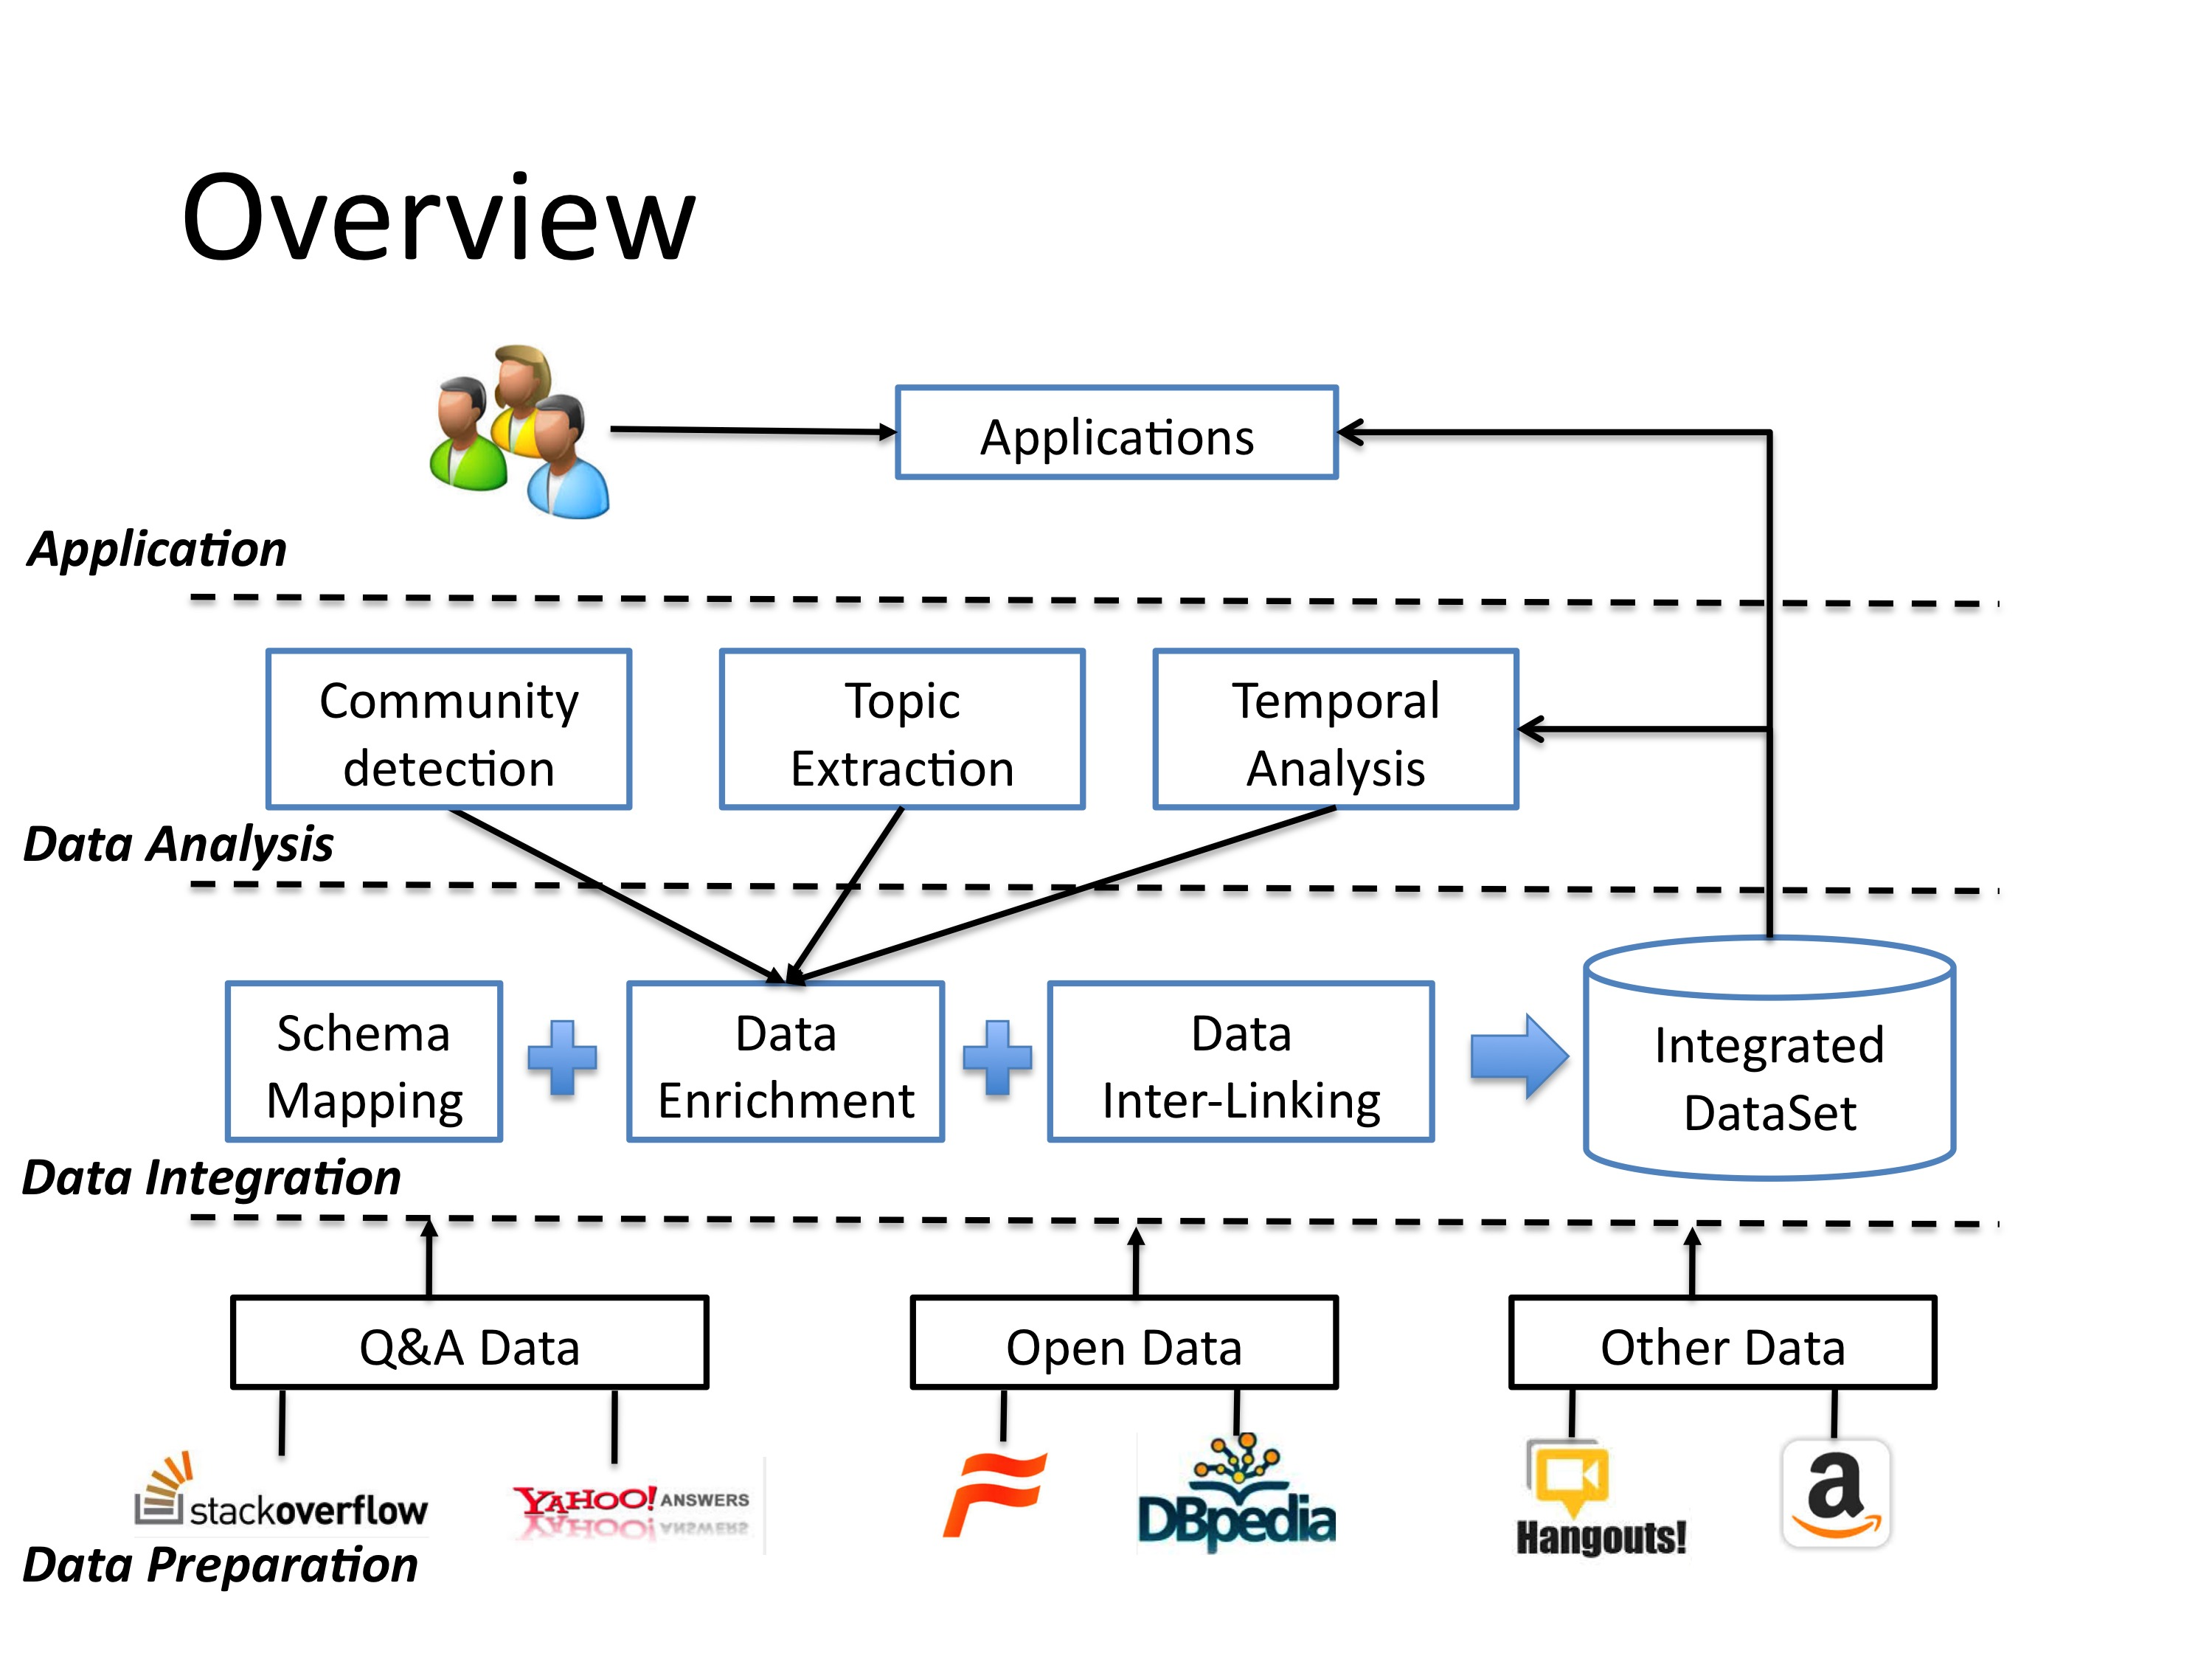
\includegraphics[width=5.5in]{framework.jpg}  
\caption{The overview of the framework proposed in this thesis to analyze Q\&A sites content and communities}
\label{fig:framework} 
\end{figure}



\section{Our Scenario: managing question-and-answer sites}


The main motivating scenario for this framework and our research questions is the case of question-and-answer sites(Q\&A sites), which is a very rich special case of user-generated content (UGC) website. Q\&A sites initially aimed at enabling users to ask questions to a community of experts. But since these exchanges are archieved as Web pages they become user-generated Web content, formulated questions with submitted answers and comments, and they can be viewed and searched again later. So people with the same or similar questions can find answers by browsing or searching the questions that were already answered. On one hand, Q\&A sites rapidly became huge repositories of question-answer content supporting highly valuable and highly reusable knowledge~\cite{anderson2012discovering}. On the other hand, Q\&A sites also gather a large number of users who keep contributing questions and answers. Most of these users are more likely to ask questions on topics they are interested in, and to answer questions on topics they are experts of. So in addition to hosting a semi-structured content network, Q\&A sites have an implicit social structure and this is why Q\&A sites are particularly illustrative of the need to jointly study both users' social structures and user-generated contents as the two sides of the same coin.
Q\&A sites are also known as Community Question Answering (CQA), indicating the combination of the two key features of Q\&A sites: a community (the users) and questions and answers (the contents).


Tags and folksonomies gathering and organizing tags are quite common features in social networks, e.g. in Twitter \footnote{\url{https://twitter.com/} (accessed Feb 2016)}, del.icio.us \footnote{\url{http://delicious.com/} (accessed Feb 2016)}, Flickr \footnote{\url{ https://www.flickr.com/} (accessed Feb 2016)}, and also in some Q\&A sites such as StackOverflow\footnote{\url{http://stackoverflow.com/} (accessed Feb 2016)}.
They are a special case of user-generated content and the activity of associating tags to content is known as collaborative tagging or social bookmarking.   
Tags enable users to classify and find resources via shared tags; they can help creating communities, considering the fact that users sharing the same tags have common interests. Besides, tags can directly reflect users vocabulary and resources annotated with the same tags often are relative to the same topics. Therefore, finding communities and topics from tags is a key question. 
We will more specifically focus on the analysis of tags associated to questions and answers in CQA sites. 


Considering again the framework we propose, a first step is the design of schemas to formalize all of the meta-information we can export from a Q\&A site. Second, the resulting dataset can be analyzes in three different ways: social structure analysis, content analysis and evolution analysis. Then the results of these analysis will be integrated to the original dataset to enrich its structure and support new usages. Third, based on this integrated dataset, we will provide several social applications, such as question recommendation, expert detection and user life-cycle management. This is the basic logic of the proposed framework and in this thesis we will focus on the export and analysis stages, and in particular on overlapping community detection, shared interest labelling and temporal analysis.


The reason why we conduct three kinds of analysis is because we believe that they address three needs linked to the two main resources in Q\&A sites: the users' network and the Q\&A content. Indeed, from a user's perspective, detecting communities of interests is useful to reveal the sub-structures of the user network and identify relevant peers. More precisely, obtaining this information can contribute to the question routing problem~\cite{li2010routing}\cite{Zhou:2012:CAQ:2187980.2188201}, which is a very important Q\&A sites optimization problem, for example, to forward a question to a user who is active in the corresponding topic and has the expertise needed to answer it.
From the content's perspective, extracting topics is required to uncover the key subjects from massive content.
It is extremely useful for instance to retrieve already posted answers to a re-submitted question.
Moreover, both users and topics are changing over time, and therefore detecting such temporal dynamics is of prime importance to be aware of novelties. These indicators also are specially usefull to community managers; they can also contribute to the community management, for instance by allowing to track the interest evolution or community evolution in Q\&A sites.



\section{Research Question: topics, communities and trends in Q\&A sites}
In this section we summarize the main research questions that this thesis will address and answer.

\subsection*{RQ1. How to formalize user-generated content?}
The information in user-generated content is unstructured. A first issue is to formalize it. In addition, once an analysis has been performed, a second issue is to formalize the detected latent information and integrate it to the initial data in order to enrich it.

\subsection*{RQ2. How can we identify the common topics binding users together?}
On user-generated content websites, users  normally are creating information about their topics of interest. It is important to be able to detect these topics from the raw content generated by the users.

\subsection*{RQ3. How can we generate a semantic label for topics?}
Until now in our research questions we haven't characterized the representation of topics and in fact a topic consists mainly of a bag of words. One essential need is to automatically generate an adequate label for each topic to convey the meaning and coverage of the topic of shared interest it represents.

\subsection*{RQ4. How can we detect topic-based overlapping communities?}
We address the problem of overlapping community detection. Unlike traditional graph-structure based methods, we try to solve this problem by relying directly on topic modeling. The advantage is that detected topics can be directly used to interpret the \textit{raison d'être} of the communities. Another reason is that, regarding our scenario, Q\&A sites support social networking, however, unlike networks such as Facebook, there are no explicit relationship-based links between their users. In fact, Q\&A sites indirectly capture the connections made by users through the question-answer links or co-answer links. The users are neither mainly concerned with nor aware of the links existing between them. The social network is said to be implicit. Therefore, compared with other classical social networks, Q\&A networks contain more \textit{star-shape} structures (many users linked to a central user) than \textit{triangle-shape} structures (users linked to each other). As a result, many community detection algorithms developed to discover sub-structures in social networks do not apply to Q\&A implicit networks. 
Moreover, people may have multiple interests i.e. they may belong to several communities of interests. It is therefore important to be able to detect overlapping communities. 

\subsection*{RQ5. How can we extract topics-based expertise and temporal dynamics?}
The topics and the interest they attract change over time. We propose to address the problem of expert detection and temporal dynamics analysis together with topic modeling. 



\section{Contributions: models to identify shared interests and temporal dynamics}
The major contributions of this thesis are as follows.
\begin{itemize}
\item{To address the research question \textbf{RQ1}, we present a model and a prototype system to extract this model of the two main resources in CQA sites: users and contents. We also present a vocabulary used to formalize the detected information.}

\item{To address the research question \textbf{RQ2}, we present a topic tree distribution method to extract topics from tags. We also propose a first-tag enrichment method to enrich questions which only have one or two tags. We show the effectiveness and efficiency of our topic extraction method.}

\item{To address the research question \textbf{RQ3}, we propose and compare metrics and provide a method using DBpedia to generate an adequate label for a bag of words capturing a topic.}

\item{To address the research question \textbf{RQ4}, based on our topic extraction method, we present a method to assign users to different topics in order to detect overlapping communities of interest.}

\item{To address the research question \textbf{RQ5}, we present a joint model to extract topic-based expertise and temporal dynamics from user-generated content. We also propose a post-processing method to model user activity. Traditionally, this information has been modeled separately.}

\end{itemize}



\section{Thesis Outline: social semantic Web and CQA sites mining}
This thesis contains a background and state of the art of related literature, an approach to detect topics from tags, an approach to detect overlapping communities and an approach to detect expertise and activities. The chapters in the rest of this thesis are organized as follows:
\begin{itemize}

\item{Chapter 2} provides a background of related domains, and the state of the art on community detection, topic modeling, expert detection and temporal analysis. We identify the research trends in the related areas, and outline the focus of this thesis.
\item{Chapter 3} describe QASM (Question \& Answer Social Media), a system based on social network analysis (SNA) to manage the two main resources in CQA sites: users and contents. We also present the QASM vocabulary used to formalize both the level of interest and the expertise of users on topics. 
\item{Chapter 4} describes an efficient approach for extracting data from Q\&A sites in order to detect communities of interest. We also present a method to enrich questions with a more general tag when they only have one or two tags. We then compare three detection methods we applied on a dataset extracted from the popular Q\&A site StackOverflow. Our method based on topic modeling and user membership assignment is shown to be much simpler and faster while preserving the quality of the detection. 
\item{Chapter 5} describes an approach to automatically generate a label for a topic by analyzing the meaning and links of its bag of words. We conduct a user study to compare different algorithms to choose the label.
\item{Chapter 6} describes a probabilistic graphical model to jointly model topics, expertises, activities and trends for a question answering Web application. We performed experiments with real-world data to confirm the effectiveness of our joint model, studying the users' behaviors and topics dynamics again on the dataset extracted from the popular question-answer site StackOverflow.
\item{Chapter 7} summarizes our contributions and describes our perspectives.
\end{itemize}



\section{Publications on the thesis contributions}
The publications resulting from this thesis are the following ones:

\begin{itemize}

\item{Journal} 


1. Zide Meng, Fabien L. Gandon, Catherine Faron-Zucker, Ge Song: Detecting topics and overlapping communities in question and answer sites. Social Network Analysis and Mining 5(1): 27:1-27:17 (2015)

2. Zide Meng, Fabien L. Gandon, Catherine Faron-Zucker: Overlapping Community Detection and Temporal Analysis on Q\&A Sites. Web Intelligence and Agent Systems 2016. 

\item{Conference Paper}

1. Zide Meng, Fabien L. Gandon, Catherine Faron-Zucker: Joint model of topics, expertises, activities and trends for question answering Web applications. IEEE/WIC/ACM Web Intelligence 2016.


2. Zide Meng, Fabien L. Gandon, Catherine Faron-Zucker: Simplified detection and labeling of overlapping communities of interest in question-and-answer sites. IEEE/WIC/ACM Web Intelligence 2015

3. Zide Meng, Fabien L. Gandon, Catherine Faron-Zucker, Ge Song: Empirical study on overlapping community detection in question and answer sites. IEEE/ACM ASONAM 2014: 344-348

4. Zide Meng, Fabien L. Gandon, Catherine Faron-Zucker: QASM: a Q\&A Social Media System Based on Social Semantic. International Semantic Web Conference (Posters \& Demos) 2014: 333-336


%\section*{backup information}








\chapter{Background}
\doublespacing
\label{chap:background}
\minitoc

%TODO FAB: please replace : web -> Web in the whole PhD
%DONE
\section{Introduction: state-of-the-art and open questions}
In this chapter, we review the related topics for the background knowledge for this thesis and provide a state of the art review of related literature. First, We introduce the background of social Web and semantic Web.
Second, we provide an introduction to the collaborative project OCKTOPUS in which this Ph.D. took place.
We then discuss the state of the art work related to community detection, topic modelling, question-answering sites, temporal analysis and our research questions.
Finally, we discuss the research trends and challenges, and we position the focus of this thesis.

\section{Social Semantic Web: combine social network analysis and Semantic Web}

\subsection{Social Web: online communities and user-generated content}
The term "social Web" was coined by Howard Rheingold in 1996. His Whole Earth Review article in 1987 introduced the notion of “Virtual Communities” and he was quoted in an article in Time magazine in 1996 introducing the term "Social Web". His website "Electric Minds", described as a "virtual community", listed online communities for users interested in socializing through the Web, saying that "The idea is that we will lead the transformation of the Web into a social Web" \cite{rheingold2000virtual}. According to the World Wide Web Consortium (W3C), "the Social Web is a set of relationships that link together people over the Web". \footnote{\url{https://www.w3.org/2005/Incubator/socialweb/XGR-socialweb-20101206/}(accessed Feb 2016)}. The social Web is designed and developed to support social interaction \cite{porter2010designing} on the Web. These on-line social interactions include for instance online shopping, blogs, forums, video sharing and social networking websites. Today, hundreds of millions of persons are using thousands of social websites to connect with friends, discover news and to share user-generated content, such as blogs, photos, microblogs, videos. By the end quarter of 2008, Facebook reported 67 million members, YouTube had more than 100 million videos and 2.9 million user channels \cite{watson2008causewired}, and these numbers are consistently growing, as today Favebook reports more than a billion of active users.  


\subsubsection{Web 2.0}
One of the significant changes for the World Wide Web was to move from the parctices of Web 1.0 to the practices of Web 2.0. The term Web 2.0 was initially coined by Darcy DiNucci in 1999 \cite{dinucci2012fragmented} and became popular through Tim O'Reilly in 2005 \cite{o2009design}. Web 2.0 techniques allowed Users to interact and collaborate with each other and create user-generated content in online community sites, while users were mostly browsing content on Web 1.0 sites. A comparison of examples of traditional Web 1.0 and Web 2.0 is hown in Figure \ref{fig:web1to2}. Popular examples of Web 2.0 sites are Facebook (social networking service), Twitter (a microblog), Youtube (A video-sharing website), Reddit (A user-generated news website).

\begin{figure}%[htbp]
\centering
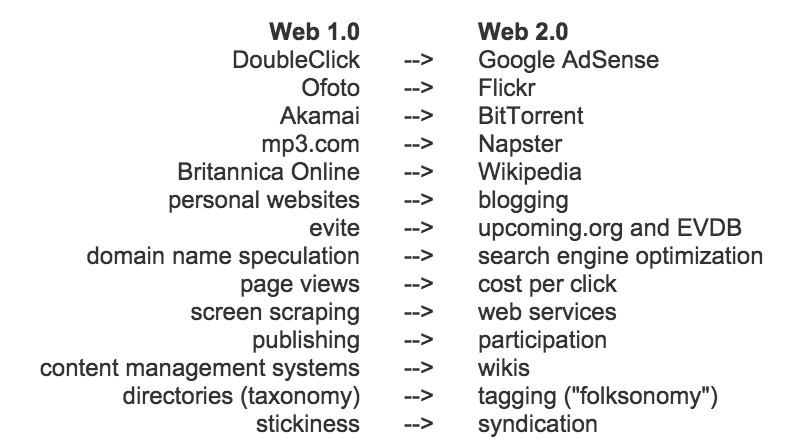
\includegraphics[width=3.2in]{web1to2.jpeg}  
\caption{A comparison of examples of Web 1.0 and Web 2.0, as in \cite{o2009design}}
\label{fig:web1to2} 
\end{figure}
With the evolution of web development technologies, such as Asynchronous JavaScript and XML (AJAX), Rich Internet Applications(RIA), Cascading Style Sheets (CSS), etc. Web 2.0 allowed users to create and share richly-typed user-generated content with each other more easily. \cite{passant2009technologies} argue that there are two main principles in Web 2.0, the first one is the \textit{"Web as a platform"}, which implies the migration from traditional desktop applications (email clients, office suites, etc.) to Web-based applications. The second one is the \textit{"architecture of participation"}, which represents how users change from data consumers to data producers in Web-based applications. For more design principles of Web 2.0 websites, we reffer the reader to \cite{o2009design} 


\subsubsection{User-generated content}
The OECD\cite{web2007web} considers that User-Generated Content (UGC) applications have the following requirements: 1) a content which is made publicly available through Internet. 2) boasting a certain level of creativity and maybe the most important point. 3) contents created outside of professional practices. UGC can be any form of content such as blog posts, photos, Q\&A, forums, tweets, videos, etc. which were created by users of an online social media websites. \cite{moens2014mining}. The reasons why people contribute to user-generated content are mainly: connecting with people, self-expression and receiving recognition. For example: users connect with friends on Facebook; users express themselves on Twitter\footnote{\url{https://twitter.com/}(accessed Feb 2016)}; users share their photos on Flickr\footnote{\url{https://www.flickr.com/} (accessed Feb 2016)}; Users ask and answer computer programming related questions on StackOverflow\footnote{\url{http://stackoverflow.com/} (accessed Feb 2016)}. 

Nevertheless, there are some issues \cite{balasubramaniam2009user} about UGC, such as: the trust problem, since the content is written by non-professionals; the privacy problem, since the content often contains or reveals private information; copyright problem, more attention should be put on protecting the right of user-generated content; etc.
For more detailed information about the driving factors and the evolution of UGC, the commercial influence of UGC, we refer the readers to \cite{balasubramaniam2009user} and \cite{smith2012does}.

\subsubsection{Question-and-Answer (Q\&A) sites}

Question-and-Answer (Q\&A) sites, also refered to as Community Question Answering (CQA) sites, initially aimed at enabling users to ask questions to a community of experts or, at least, a community of (shared) interest. Since this user-generated content, composed of questions and answers in this case, can be archived and later viewed and searched again, people with the same or similar questions can find answers by browsing or searching the questions that were already answered. For example\footnote{\url{https://en.wikipedia.org/wiki/Comparison_of_Q\&A_sites} (accessed Feb 2016)},
%TODO FAB : Naver does not appear in Wikipedia comparison
%DONE, it's naver knowledge serach
the first potential Q\&A site Naver Knowledge Search \footnote{\url{http://naver.com} (accessed Feb 2016)} launched in 2002 in Korean, has accumulated 70 million quesitons and answers, and continues to receive over 40,000 questions and 110,000 answers per day\cite{sanghunnewyork}. Baidu Knows\footnote{\url{http://zhidao.baidu.com/} (accessed Feb 2016)} and Zhihu \footnote{\url{http://www.zhihu.com/} (accessed Feb 2016)} are the most popular Q\&A sites in China. It is reported \footnote{\url{https://en.wikipedia.org/wiki/Zhihu} (accessed Feb 2016)} that the number of registered users of Zhihu had exceeded 10 millions at the end of 2013, and reached 17 millions in May 2015 with 250 million monthly page views. Yahoo Answers, lunched in 2005, offers Q\&A sites localized in 26 countries and it was said in September 2007\cite{Harper:2008:PAQ:1357054.1357191} that Yahoo Answers was estimated to have 18 millions unique visitors monthly.


As the main access means to the information on the Web are the search engines, we compare the traditional keyword-based search engine to question answer sites in terms of information retrieval tasks. In search engines, people choose some keywords to describe their problem, then look for related information in the result pages to solve their problems. In question answer site, people post their questions and wait for experts to solve it. Table \ref{tab:intro_compare} compares the two paradigms. 
\begin{table}[!hbp]
\tiny
\centering
\begin{tabular}{|p{58pt}|p{58pt}|p{58pt}|p{58pt}|p{58pt}|}
%\begin{tabular}{|c|c|c|c|c|}
\hline
& Problem define & Timely & Precise & Solution \\
\hline
Q\&A & Well organized questions and background info. & Until someone answer it & Specific to the question& directly get the answers\\
\hline
Search Engine& Well chosen keywords or short question & immediately get relevant info. & Not specific to the question& Need to analyze the results.\\
\hline
\end{tabular}
\caption{Comparison of the Q\&A and Search Engine}
\label{tab:intro_compare}
\end{table}

In a Q\&A site, people need to provide very detailed information about their questions, in order to let other users understand them. Providing additional details is even often asked by the experts in the first interactions. In a search engine, people have to wisely choose search keywords in order to look for solutions as the quality of keywords largely influences the results. When we pose a question to a Q\&A site, it takes time to attract expert users and get the answers, but the search engine can immediately return relevant information. Once people get answer from Q\&A site, normally it is very specific to the question and very precise. So Q\&A site can solve very complicated and precise questions. In search engine, people can get very relevant information about the keywords they provide but sometime, the results are very general and not specific to the question. User then have to find the solutions from these information by themselves. Beyond this comparison, it must also be stressed that as the Q\&A site grows, priding an efficient search engine for its archive becomes a specific problem at the intersection of both paradigms. Moreover, a number of results found by major search engines come from Q\&A Web archives.

On one hand, Q\&A sites became huge repositories of question-answer content which provide highly valuable and highly reusable knowledge \cite{anderson2012discovering}, \cite{Shah:2010:EPA:1835449.1835518}. On the other hand, Q\&A sites also contain a large number of users who keep contributing questions and answers. And most of them are more likely to ask questions on topics they are interested in and answer questions in topics they are experts of. This strong coupling of linked content and linked users is an aspect we will come back to.

Thus, we can consider this user-generated content is normally of high quality as it was generated by people with very strong domain knowledge and expertise. We list key features of some famous Q\&A sites in table \ref{tab:qasites}. 

\begin{sidewaystable}%[!hbp]
\centering
%\begin{tabular}{|p{46pt}|p{60pt}|p{60pt}|p{25pt}|p{60pt}|p{25pt}|}
\begin{tabular}{|c|c|c|c|c|c|c|}
\hline
& Category & Reward &  Tag & Vote &Best Answer&Dataset availability\\
\hline
Yahoo Answer\footnote{\url{https://answers.yahoo.com/} (accessed Feb 2016)} & Multiple & Level and Points & no& answer & yes & web access\\
\hline
StackOverflow\footnote{\url{http://stackoverflow.com/} (accessed Feb 2016)} &Computer Science & Reputations& yes&Both & yes& full access\footnote{\url{https://archive.org/details/stackexchange} (accessed Feb 2016)} \\
\hline
Baidu Zhidao\footnote{\url{http://zhidao.baidu.com/} (accessed Feb 2016)}& Multiple&Level and Coins & no &Both &yes&web access \\
\hline
Zhihu\footnote{\url{https://www.zhihu.com/} (accessed Feb 2016)} & Multiple & Vote and Like & yes & answer & yes& web access \\
\hline
Quora\footnote{\url{https://www.quora.com/} (accessed Feb 2016)} & Multiple&views& no & answer & no &web access\\
\hline
\end{tabular}
\caption{Key features of famous Q\&A sites}
\label{tab:qasites}
\end{sidewaystable}

%TODO FAB: (1) you need to explain the columns of the table
%DONE

The column 'Category' indicates the topics which are discussed in the websites.
The column 'Reward' indicates the rewarding system which is use encourage users' contribution.
The column 'Tag' indicates whether the website enable user to assign tags on questions.
The column 'Vote' indicate whether the website enable user to vote on question, answer or both.
The column 'Best Answer' indicate whether the website enable user to choose a best answer.




%(2) you could add other features: tags, firrent user roles, etc.
%DONE
%why we use stack over flow dataset.
% because they publish their whole dataset with all the information which could be used in our work. explained below.
StackOverflow is the most popular Q\&A site that focus on computer programming topics. They publish their dataset every months. It include all the detail information, such as quesiton answer contents, user profile, temporal information. Therefore, we mainly use StackOverflow dataset throughout this work. Figure \ref{fig:stackexample} shows a example of question and answer on StackOverflow.  
\begin{figure}%[htbp]
\centering
%\epsfig{file=fly.eps, height=1in, width=1in} % use this if you use "pdflatex"
%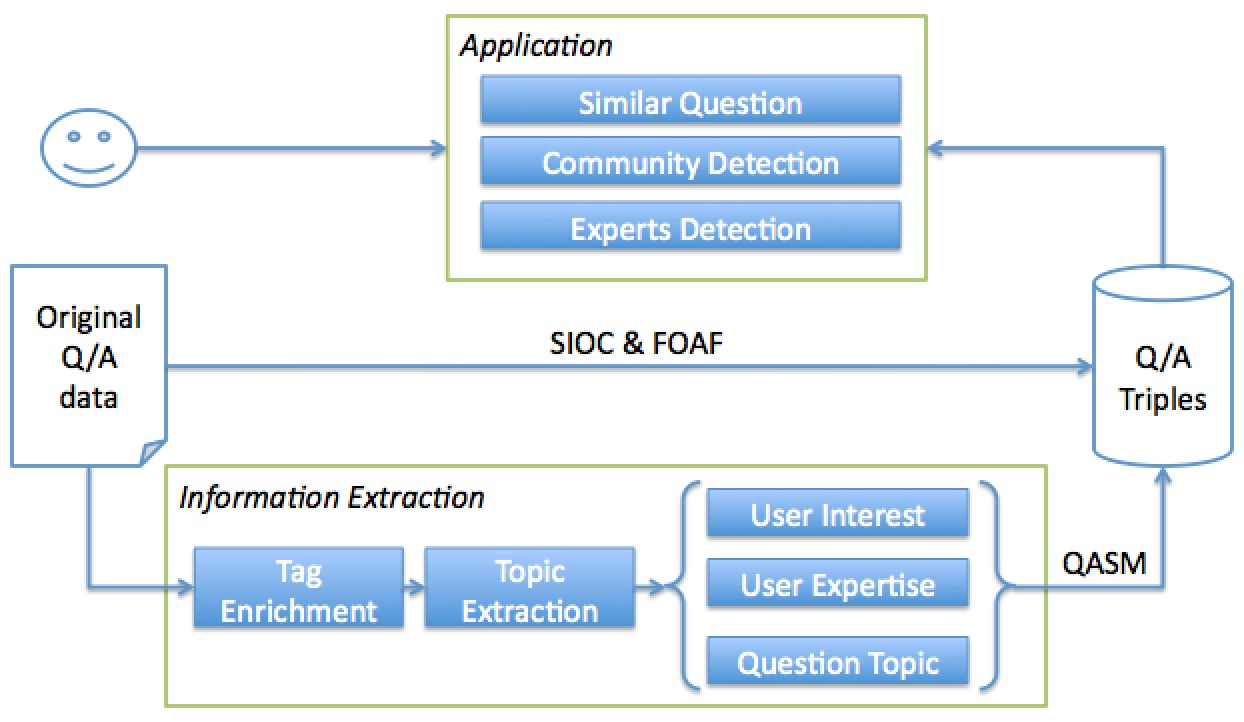
\includegraphics[height=1.857in, width=3.2in]{overview.png}  
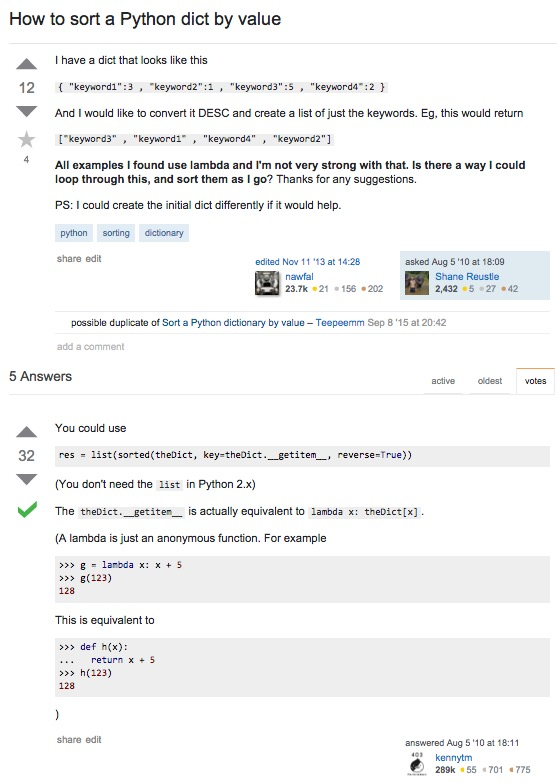
\includegraphics[width=5.3in]{stackexample.jpeg}  
\caption{A example of question and answer on StackOverflow \footnote{\url{http://stackoverflow.com/questions/3417760/how-to-sort-a-python-dict-by-value} (accessed Feb 2016)}
}
\label{fig:stackexample} 
\end{figure}

As we pointed before there are two main dimensions in Q\&A sites the coupling of which provide the power of these sites:
\begin{itemize}
\item{Social dimension:} 
A large number of people are very active and keep contributing answers to these sites. Most of them are more likely to answer questions about topics in which they are interested and specialized. Identifying interest groups of users in Q\&A sites is an interesting indication of expertize in a Q\&A and community detection is a fundamental research topic for social network analysis. Many community detection algorithms have been developed to find sub-structures in social networks. Q\&A sites are also social networks. However, unlike friendship networks such as Facebook, there are no explicit relationships between people on Q\&A sites. Besides people are not aware of who they are interacting with, and normally they do not maintain a solid relationship. People are more like isolated nodes grouped by interests and the social network remains implicit. So interest groups are an important implicit sub-structure to detect in such social sites. Moreover, people have multiple interests and therefore belong to several interest groups. Therefore an important aspect is the ability to detect overlapping communities or interest groups. 

\item{Content dimension:}
Another important resource in Q\&A sites are "question-answer" pairs. Questions cover different topics, and the fact a user asks or answers a question can reflect the fact that he/she is interested in the topics touched by that question. Therefore, detecting topics of questions and identifying interests of groups are realted problems. We want not only to detect communities, but also want to find their "raison d'\^etre" i.e. to find the topic(s) of interest shared by each detected community. Topic extraction is a critical research problem in text analysis. Many topic extraction methods have been proposed to cluster textual resources by their topics. One of the reasons why we need such content analysis is that it enables systems, for instance, to use topics in recommending similar questions or in routing questions to experts, which are both very important functionalities in Q\&A scenario.

\end{itemize}

\subsection{Semantic Web: formalizing and linking knowledge}

According to W3C, "The Semantic Web provides a common framework that allows data to be shared and reused across application, enterprise, and community boundaries"\footnote{\url{https://www.w3.org/2001/sw/} (accessed Feb 2016)} through the Web. Tim Berners-Lee \cite{berners2001semantic} also uses this term to refer to a Web of data that can be processed by machines. It is a change from a visions of a Web of documents to a Web also publishing and linking datasets. People generate and consume huge amount of data every day. However, these data are kept in silos by each application or each website, and people have to manage and process the exchange of information by themselves. For example, in order to make a trip plan, a user should check different website including flight, hotel, weather, train schedule and so on. It is even not easy for human to integrate them. For example, a small change of flight may cause user to check and change all the other reservations. It is also not possible for applications to manage all these information from different website. However, instead of web of document, if we have a web of data, then it is possible for applications to process and integrate them together. So, the main attribute of the Semantic Web is to enable content providers not only to publish human-readable Web document, but also machine-readable data. With this vision, the Semantic Web allows applications to process data from different sources the same way people gather information from different Web pages. Later in 2006, Tim Berners-Lee\cite{berners2006linked} proposed the Linked Data principles for publishing structured data on the Semantic Web. It is a method to share Semantic Web data using the Web architecture \cite{bizer2011evolving}. An important development in this context is the W3C Linking Open Data (LOD) \footnote{\url{https://www.w3.org/wiki/SweoIG/TaskForces/CommunityProjects/LinkingOpenData} (accessed Feb 2016)}. Figure \ref{fig:lod} shows the LOD cloud diagram\footnote{Linking Open Data cloud diagram, by Richard Cyganiak and Anja Jentzsch. \url{http://lod-cloud.net/}}. It shows the datasets that have been published as Linked Data. As of August 2014, the LOD cloud contains 1014 data sets classified into 8 domains while There are 520 data sets(taking 51.28\%) in the domain of Social Web and 48 data sets in User-generated content(taking 4.73\%).

%TODO Fab: latest LOD cloud version and stats are from 2014 http://lod-cloud.net/
%DONE updated

In the following subsections, we briefly introduce the RDF data model which is used to represent data on the Semantic Web and the related vocabularies to formalize social media dataset. For more details about the objectives and goals of the Semantic Web, we refer the readers to \cite{feigenbaum2007semantic} and \cite{berners2001semantic}.

\begin{sidewaysfigure}%[htbp]
\centering
%\begin{sideways}
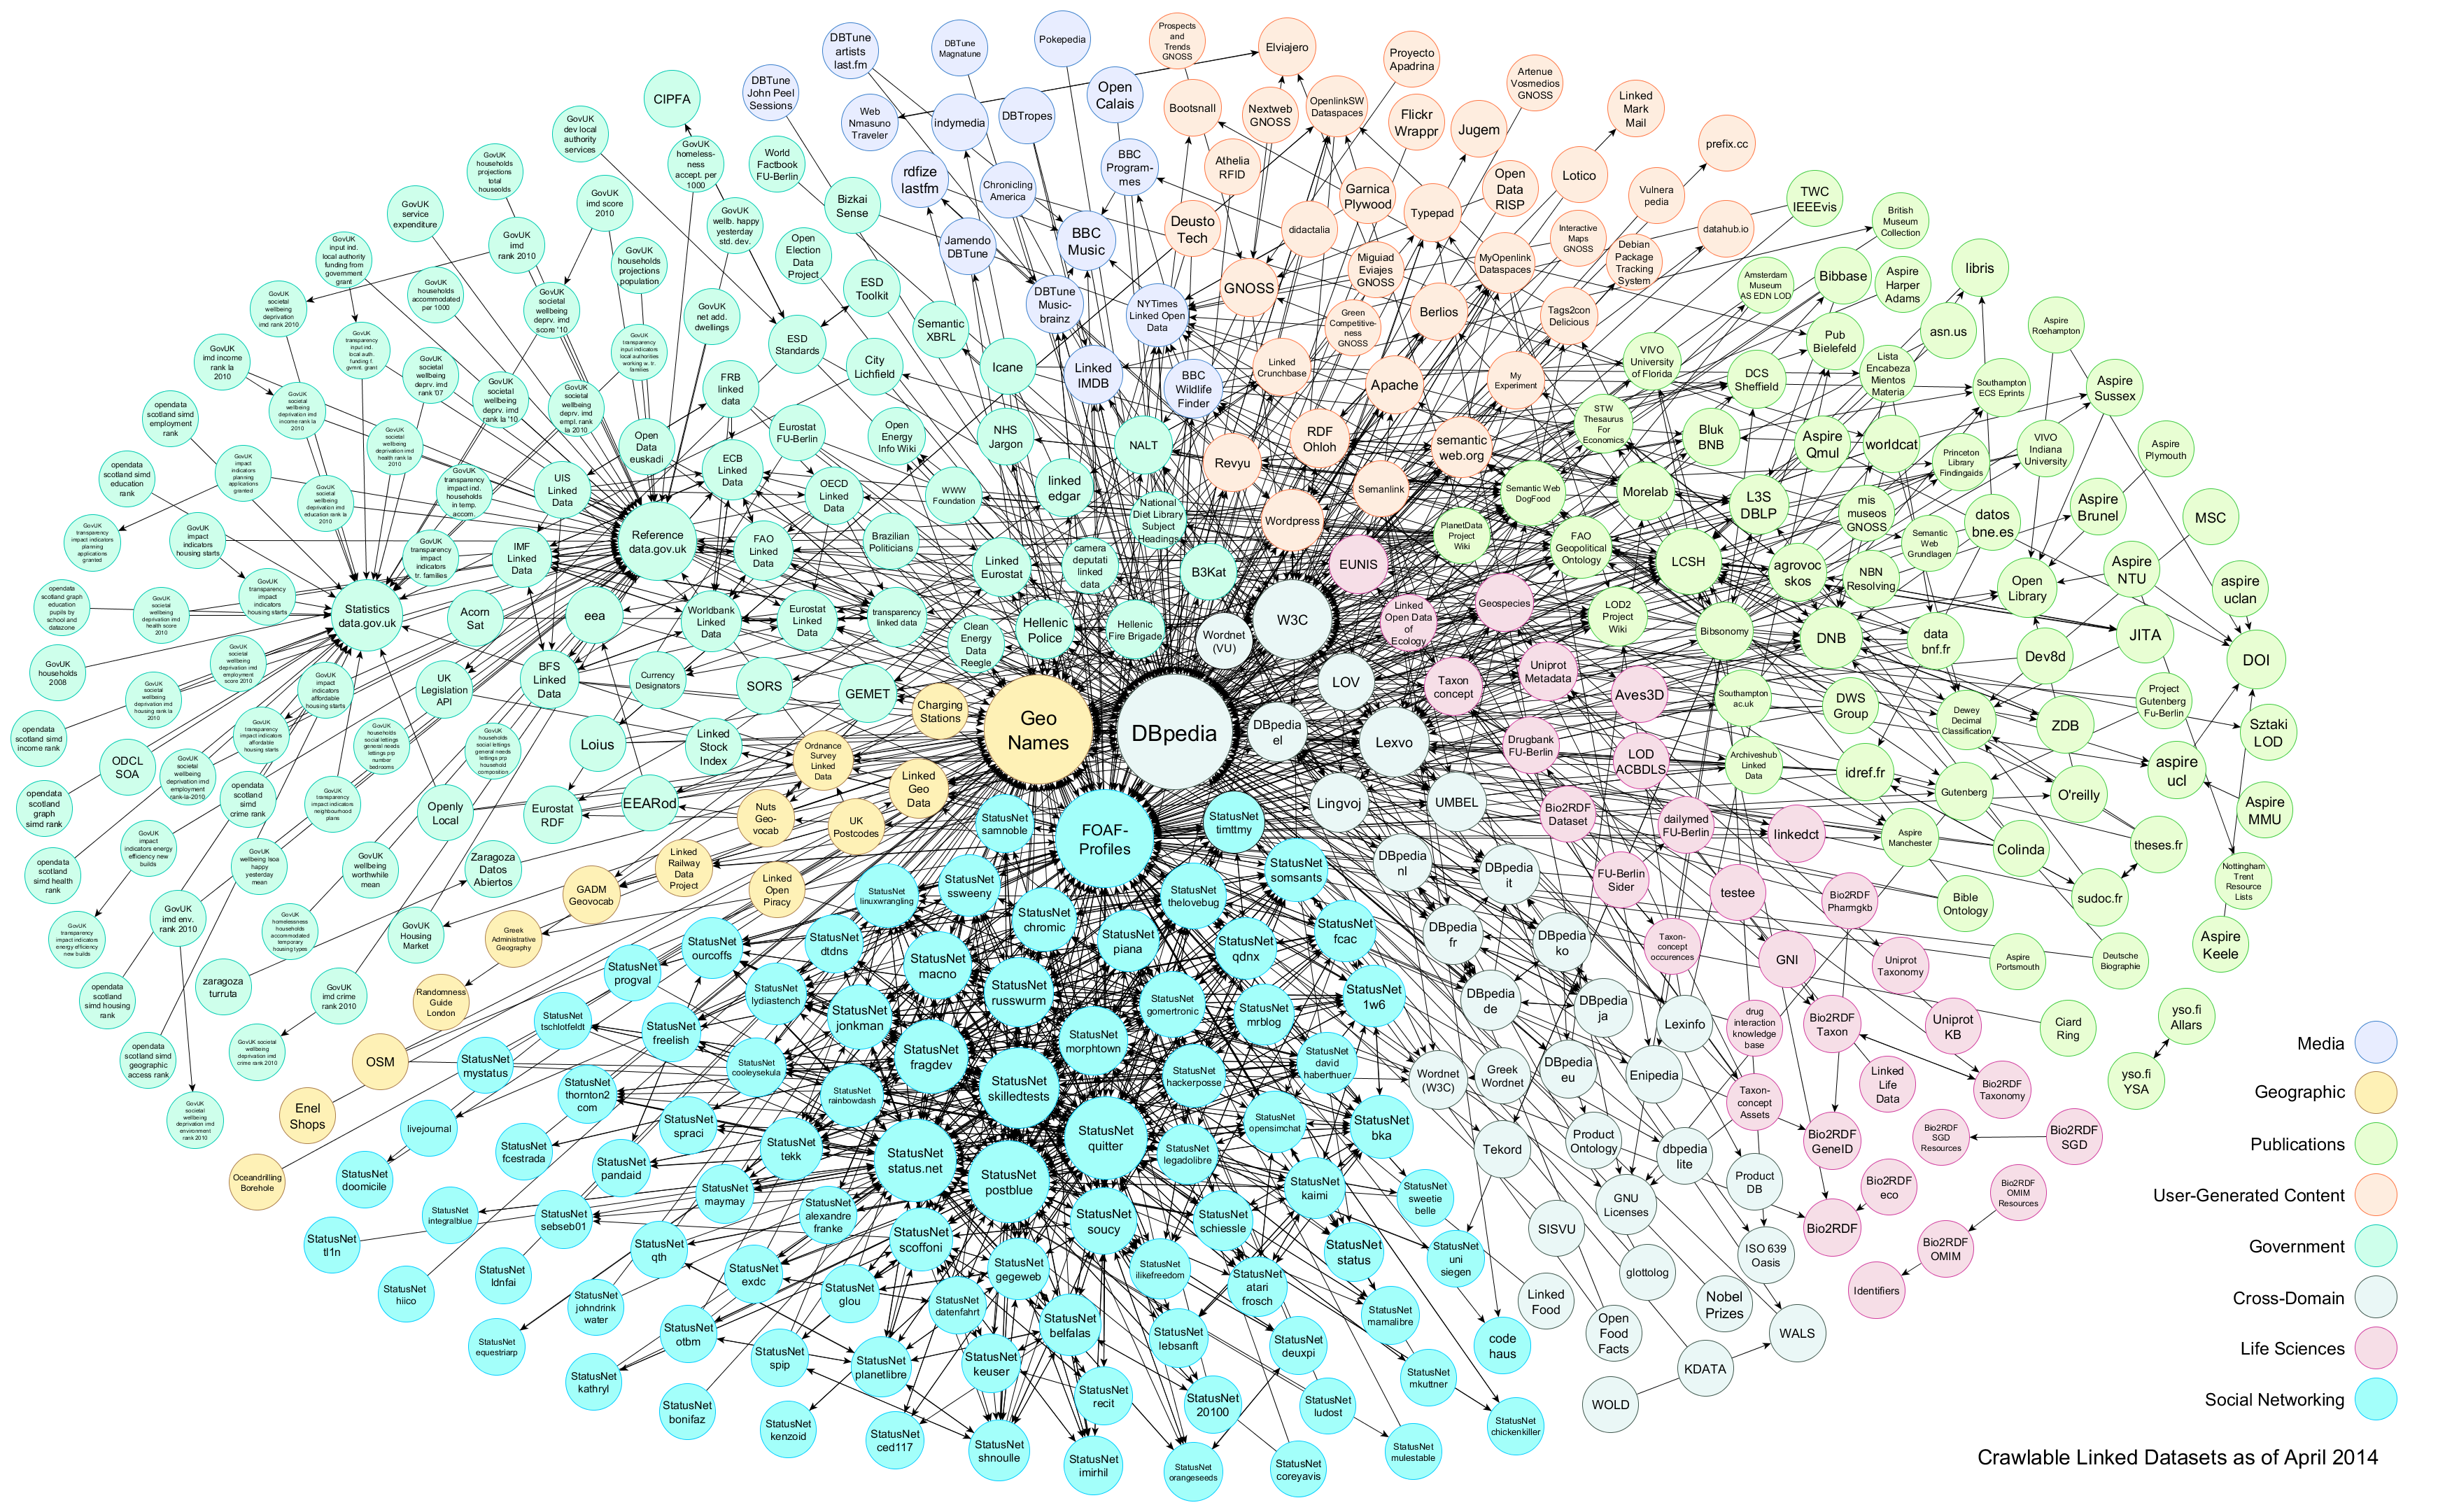
\includegraphics[width=8in]{lod2.png}  
%\end{sideways}
\caption{Linked Open Data cloud diagram.}
\label{fig:lod} 
\end{sidewaysfigure}}

\subsubsection{RDF}
The Resource Description Framework (RDF) data model is used to describe resources with \"the subject, the predicate and the object triple\", which can be viewed as "a natural way to describe the vast majority of the data processed by machines". 
%It commonly refer to " the subject, the predicate and the object triple". 
By joining triples through shared URIs RDF forms a graph data model\footnote{Resource Description Framework (RDF):Concepts and Abstract Syntax \url{https://www.w3.org/TR/2004/REC-rdf-concepts-20040210/#section-Concepts} (accessed Feb 2016)} i.e. as show in Figure \ref{fig:rdfgraph} each triple can be seen as a potentially distributed arc of an RDF oriented label multi-graph. 

\begin{figure}%[htbp]
\centering
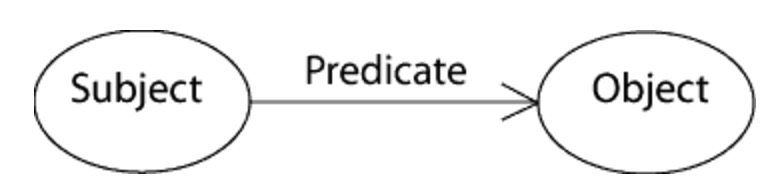
\includegraphics[width=5.3in]{rdfgraph.png}  
\caption{The triple as an arc in the graph data model of RDF.}
\label{fig:rdfgraph} 
\end{figure}

The subject represents the described resource. The predicate represents the property used to describe the resource. The object represents the value of the property for the described resource. Any user can define and describe any resource with this model. For example, to formalize a fact that a user is the owner of the question \footnote{\url{http://stackoverflow.com/questions/16772071/sort-dict-by-value-python} (accessed Feb 2016)} from a popular question answer site Stackoverflow, we can use the following triple to describe it. Where respectively: 
%TODO Fab: reformat the triple properly : the use of itemize here is not appropriate. Code style? 
%Maybe table.
%\begin{itemize}
%\item{<\url{http://stackoverflow.com/users/1214235/kingrauk}>} %\item{<\url{http://rdfs.org/sioc/ns#owner_of}>} %\item{<\url{http://stackoverflow.com/questions/16772071/sort-dict-by-value-python}> }

%\end{itemize}


\begin{itemize}
\item{<\url{http://stackoverflow.com/users/1214235/kingrauk}> is the URI that identifies the user who created the question}
\item{<\url{http://rdfs.org/sioc/ns#owner_of}> is the URI that identifies the property \textit{owner of}}
\item{<\url{http://stackoverflow.com/questions/16772071/sort-dict-by-value-python}> is the URI that identifies the question}
\end{itemize}
%TODO Fab: the previous triple does not declare a question it declares an owner (SIOC UserAccount) of a resource ; nothing more can be derived from this triple.
%DONE, yes, This triples hould be used to describe the fact that a user own a question.

Similarly, we can create another triple to formalize a fact that a answer is a reply to a question post. With respectively:
%TODO Fab: reformat the triple properly : the use of itemize here is not appropriate. Code style? 

\begin{itemize}
\item{<\url{http://stackoverflow.com/questions/16772071/sort-dict-by-value-python/16772088#16772088}> is the URI that identifies the answer to the question}
%TODO Fab: since you use SIOC it is only the reply to a post not precisely an answer to a question
%DONE, yes, just use it as an example. 
\item{<\url{http://rdfs.org/sioc/ns#reply_of}> is the URI that identifies the property \textit{reply of}}
%TODO Fab: in SIOC you can see that has_reply is the initial inverse relation
\item{<\url{http://stackoverflow.com/questions/16772071/sort-dict-by-value-python}> is the URI that identifies the question.}
\end{itemize}

Alternatively, we can also create another triple to formalize this fact where we can find the predicate 'reply\_of' is the inverse relation of 'has\_reply'. With respectively:
\begin{itemize}
\item{<\url{http://stackoverflow.com/questions/16772071/sort-dict-by-value-python}> is the URI that identifies the question.}

%TODO Fab: since you use SIOC it is only the reply to a post not precisely an answer to a question
%DONE, yes, just use it as an example. 
\item{<\url{http://rdfs.org/sioc/ns#has_reply}> is the URI that identifies the property \textit{reply of}}
%TODO Fab: in SIOC you can see that has_reply is the initial inverse relation
%DONE updated here.
\item{<\url{http://stackoverflow.com/questions/16772071/sort-dict-by-value-python/16772088#16772088}> is the URI that identifies the answer to the question}

\end{itemize}


\subsubsection{Ontologies in RDFS and OWL}
An ontology is "a set of representational primitives with which to model a domain of knowledge or discourse. The representational primitives are typically classes (or sets), attributes (or properties), and relationships (or relations among class members). The definitions of the representational primitives include information about their meaning and constraints on their logically consistent application"\cite{liu2009encyclopedia}.

RDF enables people to describe resources but does not provide the basis primitives to define properties and classes. This is the role of RDFS and OWL. From the definition given by W3C\footnote{\url{https://www.w3.org/TR/rdf-schema/} (accessed Feb 2016)}, RDFS, which is short for 'RDF Schema', is RDF vocabulary description language in order to represent RDF data. RDF Schema is an extension of the basic RDF vocabulary. Other vocabulary definition technologies, like OWL or SKOS, build on RDFS and provide language for defining structured, Web-based ontologies which enable richer integration and interoperability of data among descriptive communities. From the definition given by W3C\footnote{\url{https://www.w3.org/OWL/} (accessed Feb 2016)}, The Web Ontology Language (OWL) is a Semantic Web language designed to represent rich and complex knowledge about things, groups of things, and relations between things. RDFS enable user to express relations between things by a standard and flexible way and provide a vocabulary such as 'rdfs:subClassOf' to describe the relations. OWL include RDFS and enable user to define much more complex relations and provide a logical way to explorer implicit knowledge. 


%NOTE FAB: you need to  and Rintroduce briefly RDFS, OWL , their link to ontology and the fact they are use to define the vocabularies you introduce next.
%DONE
%NOTE FAB: then you should have a section on the vocabularies uou reuse with SIOC but also Dublin Core and FOAF no ? SKOS? when I look at section " QASM Vocabulary: formalize latent information" I think you use and could use more vocabularies than SIOC and they should all be introduced here.

\subsubsection{Vocabularies used in this thesis}
%Thus, it is necessary to define an ontology for specific domain knowledge. 
In this thesis we needed to represent users, posted questions and answers, communities, topics. Thus it is necessary to define an ontology for specific domain knowledge. We list the related and popular vocabularies used in our work.
%TODO Fab : complete this section


\textbf{SIOC}\footnote{\url{https://www.w3.org/Submission/sioc-spec/ }(accessed Feb 2016) } refers to the \textit{Semantically-Interlinked Online Communities} ontology, which provides the main concepts and properties to describe online communitiy sites, such as, weblogs, forums, message boards, wikis. These websites contain huge amount of valuable information. SIOC ontology tries to solve the problem that online community sites are like islands without bridges connecting them. It uses semantic web technologies to describe both the structure and content information in these online communities. It also allows us to link these information to related online communities. Fig \ref{fig:siocontos} shows the overview structure of SIOC ontology. It mainly formalizes community users and related activities in online communities.
 
\begin{figure}%[htbp]
\centering
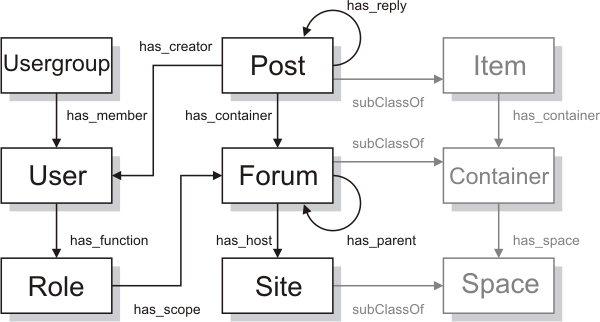
\includegraphics[width=5.3in]{sioconto.png}  
\caption{The Overview of SIOC ontology.}
\label{fig:siocontos} 
\end{figure}


%TODO Fab: complete with more descriptions
%DONE
 
The 'user' primitive in SIOC extends the \textbf{FOAF}\footnote{\url{http://xmlns.com/foaf/spec/} (accessed Feb 2016) } ontology, which is another popular ontology to describe people and relationship between people. FOAF is a project devoted to linking people and information using the Web. SIOC ontology mainly extend FOAF 'Core'. It describes characteristics of people and social groups that are independent of time and technology. It includes classes such as 'OnlineAccount', 'OnlineGamingAccount' 'Organization', and 'Person'. Compared with SIOC, FOAF is not focusing on online communities and the user-generated content aspects. 
 
\textbf{Doublin Core} \footnote{\url{http://dublincore.org/documents/dcmi-terms/} (accessed Feb 2016) } specification provides term definitions that focus on issues of resource discovery, document description and related concepts useful for cultural heritage and digital library applications. It is used to describe Web resources, such as Web pages, images, videos. It also define physical resources such as CD, books. Dublin Core Metadata may be used for multiple purposes, from simple resource description, to combining metadata vocabularies of different metadata standards, to providing interoperability for metadata vocabularies in the Linked Data cloud and Semantic Web implementations. It is also not specific for online communities and user-generated content.

\textbf{SKOS}\footnote{\url{https://www.w3.org/2004/02/skos/intro} (accessed Feb 2016)} is an area of work developing specifications and standards to support the use of knowledge organization systems (KOS) such as thesauri, classification schemes, subject heading systems and taxonomies within the framework of the Semantic Web. It can formalize the semantic relations between resources, such as 'narrower', 'boarder' and relatedd'. It can also formalize concepts and labels which are often used in online communities.
 
From the above introduction, we extend the existing work in the direction of formalizing the latent information, which  is beneath the data. For example, we can use existing work to formalize a topic. However, it is also interesting to formalize that to what extent a user is interested in a topic.
 
\section{Context of the OCKTOPUS project: find the value of user-generated content}
Over the past 15 years, along with the success of the Social Web, online communities have progressively produced massive amounts of user-generated content collaboratively.

While some of these communities are highly structured and produce high-quality content (e.g., open-source software, Wikipedia), the level of discussions found within less structured forums remains highly variable. Coupled with their explosive growth, the lower quality of structure in online open forums makes it hard to retrieve relevant and valuable answers to users' search queries, and subsequently diminishes the social and economic value of this content.

The objective of the OCKTOPUS project\footnote{\url{https://alcmeon.com/ocktopus/} (accessed Feb 2016) } is to increase the potential social and economic benefit of this user-generated content, by transforming it into useful knowledge which can be shared and reused broadly.

One of the targeted and easily-understandable output of the project is a demonstration platform which can be used to input a newly-formulated question, search online forums for a similar already-answered question, and display a unique user-generated answer associated with these similar questions.

This demonstration platform is built around the idea that finding relevant high-quality answers can be broken down in two steps:
\begin{itemize}
\item{Triage user-generated content to extract gold (knowledge structured as pairs of questions and answers) from ore (random discussions)}
\item{Given a newly-formulated question, retrieve relevant similar questions within the gold.}
\end{itemize}
OCKTOPUS therefore investigates newer data mining techniques based on the proper assessment 1) of the organizational traits of online communities, 2) of the tree-structure of online discussions, and 3) of the temporal dynamics of large typed semantic user-user graphs to help improve the automatic classification and triage of unstructured online content.



\section{Overlapping Community Detection}
We distinguish between three kinds of approaches for community detection, depending on their characteristics: Graph-based methods relying on the network structure; Clustering methods based on the similarity of user profiles; Probabilistic graphical models based on network structure and/or user profiles.

\subsection{Graph-based Methods}
A first and direct solution is to extract an implicit network structure (such as a question-answer network, a co-answer network, etc.) from interaction traces to come down to a traditional community detection problem on social networks. Since intuitively, users are grouped by interests, and most of their interactions are based on shared interests, it is reasonable to induce a network structure from these interactions and then run community detection algorithms on the network. Many classical algorithms have been developed such as~\cite{DBLP:journals/csur/XieKS13}\cite{ahn2010link}. There are many constraints when adopting these methods. First, they do not take into account node attributes nor link attributes. Take co-answer network as an example, where nodes represent users and links represent users answering the same questions. In case two users are connected, these methods can only indicate that they have answered the same questions many times. They cannot provide the information whether they have answered questions on the same topic or on different topics. Second, some of the works adopting this approach cannot detect overlapping communities, while other works such as~\cite{DBLP:journals/csur/XieKS13} address this problem.

\subsection{Clustering Methods}
Community detection can also be envisioned as a clustering problem. By computing similarities between user profiles, one can detect communities according to clustering results. The choice of the similarity metrics is quite important and influences clustering results. 
To find similar interests, we first have to define the distance between user's interests and the definition of this distance has a strong influence on the clustering results. For instance, we can consider a bag of tags with their
weights to represent an interest, then compute the weighted tag distance to define the interest distance between two users.
Clustering methods, such as~\cite{DBLP:conf/sigmod/XuKWCC12}\cite{DBLP:conf/icwsm/GargiLMY11}, group users according to their features. They do not take the network structure into consideration. Moreover, some clustering algorithms normally output hard-partition communities i.e. one user can only be assigned to one community. However, in the scenario we are interested in, a user often has more than one interest and should be assigned to more than one group simultaneously. This is a constraint for those hard-partition algorithms. 
\cite{Chang:2013} use spectral clustering to detect topics from the graph of tag co-occurrence. Compared to it, our approach is more efficient since we only run spectral clustering on a co-occurrence graph of selected tags (only 10\% of all the tags). Besides, \cite{Chang:2013} does not give any details on how to compute the topic tag distribution and user topic distribution, while we do.

\subsection{Probabilistic Graphical Models}
A third approach consists in using a probabilistic graphical model for both the user profiles and the network structure to solve community detection problem. For example, \cite{DBLP:conf/isi/ZhangQGFY07} transform links to binary node attributes, then use a Latent Dirichlet allocation(LDA) model to detect communities. \cite{journals/jasis/SunL13} use a LDA-based method on social tagging systems where users label resources with tags, but they do not consider the problem of overlapping community detection.  \cite{tang2008arnetminer} use an extended LDA-based model to analyze academic social networks in order to find expert authors, papers and conferences. A problem of these LDA-based models is that they normally assume soft-membership~\cite{yang2013community} which means that a user cannot have high probabilities to belong to several communities simultaneously. That is to say that the more communities a user belongs to, the less it belongs to each community (simply because probabilities have to sum to one). 
Moreover, \cite{mcdaid2010detecting} and \cite{lancichinetti2011finding} also use statistic model to detect overlapping communities. The difference is that LDA-based models normally integrate topic detection which can be used to interpret detected communities while the two above cited methods only detect overlapping communities without any topic information on each detected communities.

\subsection{Discussion of community detection alternatives}
Table \ref{tab:methodcomparison} summarizes the main features of the three approaches. 
The columns 'node' and 'link' indicate whether each method uses this information.  
The column 'overlapping' indicates whether a user could belong to different communities i.e. if the approach detects overlapping communities.  
The column 'membership' indicates if the method provides a measure of "how much a one user belongs to a community". 
The column 'topic' indicates if the method generate a bag of words to represent a topic, which can be used to explain the main aspects of contents generated by the users in community.

%TODO Fab: finish description above XXXXXXXXXXXXXXXXX.
%DONE
%TODO Fab: if there are differences between the methods you referenced in the three kinds of approaches you should add a line per reference in the table to show these differences.
%DONE in the summary section, I did this compartion between references. Here is just a summarizing of methods.

Graph-based approaches normally use link information while ignoring node attributes. Some of them cannot detect overlapping communities or provide membership ratios which are weights denoting to what extent a user belongs to a community. Most of these methods cannot identify the topic in each detected community. Clustering approaches use node attributes to group similar users. Some of their results are hard-partition communities, with no overlapping and no membership information. LDA-based models overcome the shortcomings of graph-based and clustering approaches, using both node attributes and link information. Besides, LDA-based models normally combine community detection with topic detection, which could be used to interpret detected communities. Our proposed method is similar to LDA-based methods, in that it also enables to detect overlapping communities and identify the topics at the same time. It differs from LDA-based methods in that it enables to consider a user having high probabilities to belong to several communities simultaneously while these methods normally assume soft-membership \cite{yang2013community}. In addition, our proposed method is much simpler and faster than LDA-based methods while preserving the quality of the detection.
For more details about community detection algorithms in graphs, we refer the readers to \cite{fortunato2010community} and \cite{DBLP:journals/csur/XieKS13}.
\begin{table}[htp]
\caption{Comparison of the main approaches and our method}
\label{tab:methodcomparison}
\centering
%\begin{tabular}{|p{28pt}|p{18pt}|p{18pt}|p{18pt}|p{25pt}|p{16pt}|}
\begin{tabular}{|c|c|c|c|c|c|}
\hline
 &uses nodes &uses links & overlap & membership & topic\\
\hline
Graph-based & no & yes & few & few &no\\
\hline
Clustering methods & yes & no & few & few &no\\
\hline
Probabilistic graphical model& yes & yes & yes & yes &yes\\
\hline
%\hline
\end{tabular}
\end{table}



\section{Topic modeling: uncover the hidden thematic structure}

According to David M. Blei\footnote{\url{https://www.cs.princeton.edu/~blei/topicmodeling.html} (accessed Feb 2016)}, "Topic models are a suite of algorithms that uncover the hidden thematic structure in document collections. These algorithms help us develop new ways to search, browse and summarize large archives of texts." For example, "guitar" and "music" will appear more often in documents about music, "law" and "lawsuit" will appear more often in documents about laws, and "the" and "is" will appear equally in both documents. A document normally contains multiple different topics in different proportions. For example, a document, which is related to music copyright lawsuit, could be talking 30\% about music and 70\% about laws.

Latent Semantic Analysis (LSA or LSI)\cite{chp2deerwester1990indexing} \cite{chp2landauer1997solution} is an early topic model based on the factorization of document-word occurrence matrix. By using singular value decomposition (SVD), it can find a linear combination of topics for each document.
Probabilistic Latent Semantic Analysis (PLSA), also known as Probabilistic Latent Semantic Indexing (PLSI)\cite{chp2papadimitriou1998latent} \cite{chp2hofmann1999probabilistic} is a generative statistic model to estimate a low-dimensional representation of the observed variables. Latent Dirichlet Allocation (LDA)\cite{blei2003latent} is also a generative statistic model that uses observed variables to explain unobserved latent variables, which is a generalization of PLSI model. \cite{griffiths2004finding} \cite{chp2griffiths2002probabilistic} use Gibbs sampling to infer the latent variables in LDA model and introduce some applications of LDA model. Many other topic models are extensions of the LDA model. For example, Hierarchical latent Dirichlet allocation (HLDA)\cite{chp2DBLP:conf/nips/2003} is a topic model that finds a hierarchy of topics. The structure of the hierarchy is determined by the data. Dynamic topic models (DTM)\cite{chp2blei2006dynamic} discover topics that change over time and how individual documents predict that change. Correlated Topic Models(CTM)\cite{chp2blei2006correlated} discover correlation structures between topics. And so on.

Topic modeling is an active field in text mining and machine learning and we refe readers to \cite{chp2Blei:2012:PTM:2133806.2133826} for a high level view and summary of the topic modeling research area and also for several exciting future research directions. One of them is : \textit{"One direction for topic modeling is to develop evaluation methods that match how the algorithms are used. How can we compare topic models based on how interpretable they are?"}.

Another interesting research problem related to topic modeling is how to automatically label the generated topics \cite{chp2cano2014automatictopiclabeling} \cite{chp2hulpus2013unsupervisedtopiclabeling} \cite{chp2aletras2014labelling} \cite{chp6OnConceptualLabelingOfBagOfWords} \cite{chp2lau2011automaticlabeling}. Typically, users of topic modeling approaches have to interpret the results and manually generate labels for topics for further processing, classification, visualization or analysis. Therefore, in this context, "labelling" means the problem of finding one or more phrases, or concepts, which can sufficiently cover, represent or describe the topic. The problem then is defined as the automation of the topic labelling.

%NOTE FAB: the following sentence is disconnected from the rest of the text and we don't know why you mention this : you have to provide a link with the previous paragraph.
%DONE, yes, you are right, I remove it.  it's disconnected with the context.


\section{Research questions related to Q\&A sites}
\subsection{Expert Detection: find the "core" user}
Research related on expert identification in Q\&A sites is mainly based on link analysis and topic modeling techniques. The general purpose of expert detection is normally to support the question routing task which essentially consists in finding the most relevant experts to answer a newly submitted question. 

\cite{zhang2007expertise} is not specific to Q\&A community and focuses on a boarder website category: help-seeking websites. It tested pagerank and hits algorithm to detect expert in such websites. Pagerank and Hit are well known authority algorithm in directed graph analysis. By constructing a directed graph of the users'network, they could apply these algorithms to find the most import node in the graph according to these centrality metrics. Besides, they proposed the Z-score measure to evaluate expertise. Compared with simple statistic measures, for instance the number of best answers user provided, the Z-score measure uses both the number of questions and the number of answers a user posted. Similarly, \cite{jurczyk2007discovering} use the HITS algorithm to discover authorities users. \cite{li2010routing} propose a probability model to estimate users' expertise for question routing task. 

\cite{chp2Zhou:2012:TPM:2396761.2398493} address a core problem in applying the previous techniques to Q\&A site. They argue that most of the previous works in expert finding are based on link analysis while ignoring the topical similarity among users and user expertise and user reputation. They proposed a topic-sensitive probabilistic model to find experts in Q\&A sites. This model is based on LDA which is widely used in topic modeling. Then they generate a topic-similar graph based on the result of topic model. Finally a PageRank algorithm is applied to find the experts. They compared their work with many state of the art link analysis algorithm and showed a gain in the experiment.

\cite{chp2Pal:2010:Expert:evolution} on the otherside proposed a temporal pattern based expert detecting method. The temporal pattern is based on the reputation system of Q\&A sites where user that has a high reputation is considered as an expert. Their approcah uses a supervised learning algorithm to distinguish expert from normal user. The limitation of this work is it cannot find in which topics are people specialized.

\cite{chp2Bouguessa:2008:Identify:authority:indegree} proposed a method using link analysis techniques to find a list of expert users based on the in-degree of authority, which is computed by the number of best answers provided by a user. Then they use Bayesian Information Criterion (BIC) to estimate the authority score of a user. Therefore, experts are chosen according to their authority score. Their expertiment was done on Yahoo Answers.


Rather than detecting global experts, another kind of works uses topic models to detect topic level experts. \cite{guo2008tapping} proposed a generative model by leveraging the category information of questions on certain Q\&A sites. \cite{yang2013cqarank} jointly model topics and expertise by  integrating a Gaussian Mixture Model to capture vote information. \cite{Chang:2013} propose a spectral clustering based topic model. %rather than the usual LDA-based model.
\cite{ma2015tri} propose a generative model to model the triple role of users (as askers, answerers, and voters). Our contribution extends this line of work. 

There are also approches applying machine learning techniques to perform expert detection. \cite{ji2013learning} combine topic models outputs and statistic features and apply a pair-wised learning to obtain a ranked model and recommend expert users for a question. \cite{pal2011early} apply machine learning algorithms to identify experts from their early behavior. \cite{anderson2012discovering} perform an in-depth study of StackOverflow\footnote{\url{http://www.stackoverflow.com/} (accessed Feb 2016)} and show that expert users tend to answer questions more quickly and gain high reputation by higher activity. Their work is based on features extraction and machine learning algorithms to predict whether a question has a long-term value and whether a question has been sufficiently answered. Their results show that votes information can indicate a user's expertise level while currently, this kind of work normally relies on the outputs of topic models.

\subsection{Question Routing: recommend new questions to users}

\cite{Guo:2008:TPQ:1458082.1458204} %UQA
try to solve question routing problem, which we categorized as Q5. They proposed an LDA-like probability model to find the latent topic of users and latent topic of questions and answers. Then based on this topic information, they can route a new question to a user which has the same topic distribution.
\cite{yang2013cqarank} %TEM
proposed a Topic Expertise Model which is also an LDA-like probability model but combined with a Gauss Mixture Model (GMM) model to detect experts in Q\&A sites. The probability model is mainly used for extracting topics from tags and words in Q\&A and it contains two LDA processes: 'user-topic-tag' and 'user-topic-content'. The GMM is used for analyzing users expertise on each topics. The output includes topic-tag distribution, user-topic distribution, topic-word distribution and the users' topic-expertise matrix. Then according to these outputs, they can identify the top tags of a topic, top users of a topic and top experts of a topic. The experiments show they can outperform the state-of-the-art probability model in Q\&A sites.


\cite{Chang:2013}
proposed a recommendation model, which integrates topical expertise and availability of users, to recommend reactive answerers and commenters for a question. It constructs a similarity matrix between tags, and runs spectral clustering algorithm over it. Then a cluster of tags can be viewed as a topic. But unlike LDA, spectral clustering can not output the topic-tag distribution which will limit the flexibility of afterwards application. The paper proposed a question-topic distribution, but it dose not mention how to compute it. So the conclusion that spectral clustering can out perform LDA is not clear. And spectral clustering is hard partition of tags, while LDA can give proportion that a tag belong to a topic. 



\subsection{Similar Question: find questions which has been answered}

\cite{anderson2012discovering} investigate the general characteristics of the Stack Overflow dataset. A contribution of this work is to predict the long-term value of a question. They find strong evidences that only 37\% of favorites for a question arrive within the time frame when the question is being answered. Actually the content in Q\&A sites mainly serves two kinds of people: the people who ask questions and the people who search through previous questions. So, if a question has a long-term value, it is more likely to be searched for again. We categorize this work as Q4 since finding out these questions could improve the result of searching for similar questions. They developed four categories of features for learning. They include: 4 questioner features which are related to questioner's behaviors; 8 activity and Q/A quality measures which are extracted from questions and answers; 8 community process features which are related the reputation of answers; and 7 temporal process features which are generated from the time information of the Q/A activity.
Then they treat this problem as a binary classification task and use a machine learning technique to predict whether a question has a long-term value. They compare their work with a baseline which only uses upvote and downvote features. 

\cite{chp2jeon2005finding}
discuss methods for question retrieval that are based on using the similarity between answers. It proposed a translation-based retrieval model to find similar questions. The experiment shows that it's possible to find semantically similar questions with relatively few overlapping words.
%NOTE FAB: I replaced "litter" by "few" becaus I thought you meant "little"
They found question titles can provide the best performance for retrieving similar question. This work is based on the intuition that most of the people don't check whether their question has been already asked which leads to a situation where there can be many semantically identical questions. Therefore, they use the similarity between answers to group similar questions. A translation model based algorithm is proposed to calculate the similarity between answers. For example, this model can provide a similarity score between 'bmp' and 'jpg'. Experiments show that the model can out perform other language models and similarity metrics. 
Table \ref{tab:workcompare} list the comparison of the above works.

%subsubsection{Probabilistic Question Recommendation for Question Answering Communities}
\cite{chp2Qu:2009:WWW:PLSA:SimlarQ} 
present a probabilistic latent semantic analysis (PLSA) approach to compute the probability a user answer will a question. They actually build a user-interest-question model. PLSA and LDA are quite similar and both are topic models, and LDA could be viewed as an extension of PLSA. The experiment shows that topic features based similarity can outperform cosine distance based similarity. \cite{chp2Wu:2008:PLSA:SimlarQ} also used PLSA to recommend questions.

%NOTE FAB: I changed the following table to a "sidewaystable" without tiny you should do that for any large table
\begin{sidewaystable}%[!hbp]
%\tiny
\centering
\begin{tabular}{|c|c|c|c|c|c|c|}
\hline
&Expert & Routing &SimilarQ& Methods & Dataset &Topic   \\
\hline
\cite{chp2jeon2005finding} 2005&no&no&yes&Probability Model&Naver\footnote{A leading Q\&A sites in South Korea} & no \\
\hline
 \cite{zhang2007expertise} 2007& yes &no& no& PageRank,Hits&Forum&no  \\
\hline
\cite{Guo:2008:TPQ:1458082.1458204} 2008 & no&yes&no&LDA based&StackOverflow&yes\\
\hline
\cite{chp2Qu:2009:WWW:PLSA:SimlarQ} 2008,\cite{chp2Wu:2008:PLSA:SimlarQ}2008  & no&yes&yes&PLSA&Yahoo,Wenda & yes \\
\hline
\cite{chp2Bouguessa:2008:Identify:authority:indegree} 2008 & yes&no&no&Link Analysis&Yahoo&no\\
\hline
\cite{chp2Pal:2010:Expert:evolution} 2010&yes&no&no&Supervise Learning&StackOverflow&no \\
\hline
\cite{anderson2012discovering} 2012& no&no&yes&Supervise Learning&StackOverflow&no \\
\hline
\cite{chp2Zhou:2012:TPM:2396761.2398493} 2012 & yes & no & no&LDA based &StackOverflow&yes\\
\hline
\cite{yang2013cqarank} 2013& yes&yes&yes& LDA based&StackOverflow&yes   \\
\hline
\cite{Chang:2013}2013 & yes&yes&no& SpectralClustering&StackOverflow&yes  \\
\hline

\end{tabular}
\caption{Comparison of several works in Q\&A sites. Expert denote 'Expert detection', Routing denote 'Question Routing', Similar denote 'Similar Question Finding', Methods denote 'Proposed algorithm', Dataset denote 'Experiment Data' Topic denote 'Topic Detection'}
\label{tab:workcompare}
\end{sidewaystable}


\section{Temporal Analysis: integrate temporal analysis with topic}

There is an increasing research interest for the temporal modeling of online communities and several methods have been proposed. 

\cite{wang2006topics} introduced \textit{Topic Over Time} (TOT), which jointly models topics and timestamps by assuming that words and timestamps are both generated by latent topics. Therefore, the parameter estimation is able to discover topics that simultaneously capture word-word co-occurrences and word-timestamps co-occurrences. If some words co-occurre for a short period, their approach will create a topic with a narrow time distribution. If some words co-occurre across a long time, their approach will create a topic with broad time distribution. The novelty of TOT  is that it treats time as an observed continuous variable rather than a Markov process. Besides, the meaning of topics remain constant while the topic itself changes over time. 
\cite{chp2blei2006dynamic} proposed a dynamic topic model that treats the temporal dimension as a Markov process where the meaning of topics changes over time. \cite{chp2onlineldaalsumait2008line} also studied topic changes over time, but they focus on proposing an online method to extract topics from a stream of data.
%NOTE FAB: I replaces dataset by data...
\cite{chp2wang2007mining} address the problem of mining correlated busty topic patterns from coordinated text streams (e.g. the same news in different medias or in different languages). They proposed a mixture model which is an extension of PLSA\cite{hofmann1999probabilistic} model to detect topic evolution from text streams by comparing topics in consecutive time intervals. 
\cite{chp2yao2010detecting} and \cite{chp2yao2012bursty} proposed a sliding window and graph partition based approach to detect burst event/topic in tags. 
\cite{chp7diao2012finding} proposed a TimeUserLDA model to find bursty topic from microblogs. It considers both user personal topic trends and global topic trends and detect bursty topics from the extracted topics over time distribution.
\cite{yin2013unified}  proposed a PLSA-based\cite{hofmann1999probabilistic} model to separate temporary topics from stable topics. Temporal topics are on popular real-life events, e.g. breaking news. It will lead to a burst in on online community discussions with a large amount of user-generated content in a short time period. Stable topics are often users' regular interests and daily routine discussions which always exist and do not evolve a lot in a long time period. \cite{hu2014user} jointly model latent user groups and temporal topics to detect group-level temporal topics.

Compared with these works, our model not only captures topics and expertise, it  can also detect topic dynamics both at the global community level and at the individual user level. Besides, we propose a post-process method to extract both topic-time and time-topic distribution. The time-over-topic distribution are usually ignored.

\section{Summary: the focus of this thesis}
We position our work regarding to each research question. 

\subsection {How to formalize user-generated content? }
    
    \begin{table}[htp]
        \centering
        \begin{tabular}{c c c c c}
        &
        \begin{turn}{270}
            \cite{chp2socialsemanticminingDBLP:series/synthesis/2015Omitola} \end{turn} 
        &
        \begin{turn}{270} 
            \cite{chp2siocontoDBLP:conf/atal/PassantBBD09}
        \end{turn}
        &
        \begin{turn}{270} 
            \cite{chp2usermodelingplumbaum2015user}
        \end{turn}
        &
        \begin{turn}{270}
        our work
        \end{turn}
        \\ \hline
        Social media mining & yes & yes & no & yes \\ \hline
        User Behaviour modeling & yes & yes & yes &yes \\ \hline
        User interesting modeling & no &yes & no & yes\\ \hline
        User activity modeling & no & no & no & yes\\ \hline
        User expertise modeling & no & no & no & yes \\ \hline
        Topic based modeling & yes & no & no &yes \\ \hline
        \end{tabular}
        \caption{Position of our work regarding to the first research question}
        \label{tab:rq1compare}
    \end{table}
    Compared with existing work, we use social media mining techniques to extract topical dynamic, topical activity, topics and topical expertize from user-generated content. Then we integrate these extracted information into the original data set in order to provide more functionality for further use. We will detail this work in Chapter \ref{chap:qasm}. 
    


\subsection{How can we identify the common topics binding users together?}
    
    \begin{table}[htp]
        \centering
        \begin{tabular}{c c c c c c}
        &
        \begin{turn}{270}
            \cite{blei2003latent} \end{turn} 
        &
        \begin{turn}{270} 
            \cite{Chang:2013} 
        \end{turn}
        &
        \begin{turn}{270} 
            \cite{yang2013cqarank}
        \end{turn}
        &
        \begin{turn}{270}
            \cite{hu2014user}
        \end{turn}
        &
        \begin{turn}{270}
        our work
        \end{turn}
        \\ \hline
        Model & PGM & SC & PGM & PGM & SC\\ \hline
        Simplicity & no & yes & no & no & yes\\ \hline
        Sub-topic & no & no & no & no &  yes \\ \hline
        Iterations & yes & no & yes& yes & no \\ \hline
        
        \end{tabular}
        \caption{Position of our work regarding to the first research question, \textit{PGM}: Probabilistic Graphical Model, \textit{SC}: Spectral Clustering}
        \label{tab:rq2compare}
    \end{table}
    
    Compared with existing work, we focus on the simplicity and efficient aspect. Based on a prefix-tree structure, our method can also extract sub topics from a topic. We detail this work in Chapter \ref{chap:ttd}.
    
    
    
\subsection{How can we generate a semantic label for topics?}



   \begin{table}[htp]
        \centering
        \begin{tabular}{c c c c c c}
        &
        \begin{turn}{270}
            \cite{chp6OnConceptualLabelingOfBagOfWords} 
        \end{turn} 
        &
        \begin{turn}{270} 
            \cite{chp2hulpus2013unsupervisedtopiclabeling} 
        \end{turn}
        &
        \begin{turn}{270} 
            \cite{chp2cano2014automatictopiclabeling}
        \end{turn}
        &
        \begin{turn}{270}
            \cite{chp2aletras2014labelling}
        \end{turn}
        &
        \begin{turn}{270}
        our work
        \end{turn}
        \\ \hline
        Extra information& Probase\footnote{\url{http://research.microsoft.com/en-us/projects/probase/} (accessed Feb 2016)} & DBpedia & no  & Bing\footnote{\url{https://www.bing.com/} (accessed Feb 2016)} results & DBpedia \\ \hline
        Method & MDL & DR Graph &S& Words Graph & DR Graph   \\ \hline
        User Study & no & yes & no & no&  yes \\ \hline
        Label Type & word & DR & word & words & DR \\ \hline
        
        \end{tabular}
        \caption{Position of our work regarding to the third research question, \textit{MDL}: Minimum Description Length, \textit{DR}: DBpedia Resource, \textit{S}: Summarization Algorithm,  }
    
        \label{tab:rq3compare}
    \end{table}
    
    Compared to the existing work, we focus on extending our topic extraction and using DBpedia resources to automatically generate labels for bags of words composing topics. We also compare several graph centrality metrics to generate labels. We describe this work in Chapter \ref{chap:label}.
    
    
\subsection{How can we detect topic-based overlapping communities?}



    \begin{table}[htp]
        \centering
        \begin{tabular}{c c c c c c c}
        &
        \begin{turn}{270}
            \cite{raghavan2007near} 
        \end{turn} 
        &
        \begin{turn}{270}
            \cite{DBLP:journals/csur/XieKS13} 
        \end{turn} 
        &
        \begin{turn}{270} 
            \cite{girvan2002community}
        \end{turn}
        &
        \begin{turn}{270} 
            \cite{yang2013community}
        \end{turn}
        &
        \begin{turn}{270}
            \cite{hu2014user}
        \end{turn}
        &
        
        \begin{turn}{270}
        our work
        \end{turn}
        \\ \hline
        Method &LPA & LPA & HC & PGM &PGM & SC\\ \hline
        Info  & Graph & Graph &Graph & Graph, Content & Graph, Content& Graph, Content\\ \hline
        Interpret& no & no & no & yes & yes & yes \\ \hline
        %explained by topic
        Overlapping & no & yes & no & yes & yes & yes \\ \hline
        Simplicty & yes & yes & yes & no & no & yes \\ \hline
        \end{tabular}
        \caption{Position of our work regarding to the first research question, \textit{LPA}: Label Propagation Algorithm \textit{PGM}: Probabilistic Graphical Model, \textit{HC}: Hierarchical Clustering \textit{SC}: Spectral Clustering}
        \label{tab:rq4compare}
    \end{table}
    Compared to the existing work, we focus on extending topic extraction methods and applying it to effectively detect overlapping communities. We describe this work in Chapter \ref{chap:ttd}.



    
\subsection{How can we extract topics-based expertise and temporal dynamics?}
    
    
        \begin{table}[htp]
        \centering
        \begin{tabular}{c c c c c c c c}
        &
        \begin{turn}{270}
            \cite{yang2013cqarank} 
        \end{turn} 
         &
        \begin{turn}{270}
            \cite{Chang:2013}  %sc
        \end{turn} 
        &
        \begin{turn}{270} 
            \cite{guo2008tapping} %uqa
        \end{turn}
        &
        \begin{turn}{270} 
            \cite{blei2003latent} %lda
        \end{turn}
        &
        \begin{turn}{270}
            \cite{hu2014user} %grostot
        \end{turn}
        &
        \begin{turn}{270}
            \cite{chp7diao2012finding} %fb
        \end{turn}
        &
        \begin{turn}{270}
        our work
        \end{turn}
        \\ \hline
        Model & PGM &SC & PGM & PGM & PGM & PGM& PGM\\ \hline
        Topic Dynamic & no & no & no & no & GL & GL,UL & GL, UL \\ \hline
        Expertise & yes & yes& no & no & yes &no &yes   \\ \hline
        User Activity& no & non-topical & no & no &topical & topical & topical \\ \hline
        \end{tabular}
        \caption{Position of our work regarding to the first research question, \textit{PGM}: Probabilistic Graphical Model, \textit{SC}: Spectral Clustering, \textit{GL}: global level, \textit{UL}: user level}
        \label{tab:rq5compare}
    \end{table}
    Compared to the existing works, we integrate topic dynamics, users' activity and topic based expertise extraction together to solve several tasks related to question answer site. We describe this work in Chapter \ref{chap:ttea}

    














\chapter{QASM: Question and Answer Social Media}
\doublespacing
\label{chap:qasm}
\minitoc

\section{Introduction: formalizing and linking knowledge on Q\&A sites}
Community Question Answering (CQA) services provide a platform where users can ask expert for help. Since questions and answers can be viewed and searched afterwards, people with similar questions can also directly find solutions by browsing this content. Therefore, effectively managing these content is a key issue. 

In order to using semantic web technology, there are two basic steps, formalizing and linking. The first one is to formalize unstructured data into structure data using domain ontology. This chapter is focus on this step. The second one is to link to open knowledge base. We introduce this step in Chapter \ref{chap:label}

We think that there are two kinds of information in our scenario. The first one is original user-generated content, for instance, question answer contents. Another one is latent information extracted by data mining techniques, for instance, topic or community information. It is important to formalize both of them. SIOC ontology is the most popular vocabulary to formalize online community, but it does not support to formalize the latent information extracted by data mining techniques. 

In this chapter, we describe QASM (Question \& Answer Social Media), a prototype system based on social media mining and semantic web technology to manage the two main resources in the CQA sites: users and contents. We also present the QASM vocabulary used to formalize both the level of interest and the expertise of users on topics. Then we present our method to extract these latent knowledge from the CQA sites. 


\section{QASM System Description: managing knowledge}
\subsection{Overview: combine social media mining and semantic web}
Figure \ref{fig:overview} presents an overview of QASM. We first use the SIOC ontology\footnote{http://sioc-project.org/ontology} to construct an RDF dataset from social media data extracted from a CQA site. Then we use social media mining techniques to extract topics, interests and expertise levels from this dataset. We formalize them with the QASM vocabulary and enrich our RDF dataset with these latent knowledge. As a result, we provide an integrated and enriched Q\&A triple store which contains both user interests, levels of expertise and topics learned from question tags. Finally, we linked our dataset with DBpedia (through named entity identification). 

Based on the QASM RDF dataset, we can provide the users of the Q\&A site with several services to find relevant experts for a question and to search for similar questions. We detail them in the following subsections.

\begin{figure}%[htbp]
\centering
%\epsfig{file=fly.eps, height=1in, width=1in} % use this if you use "pdflatex"
%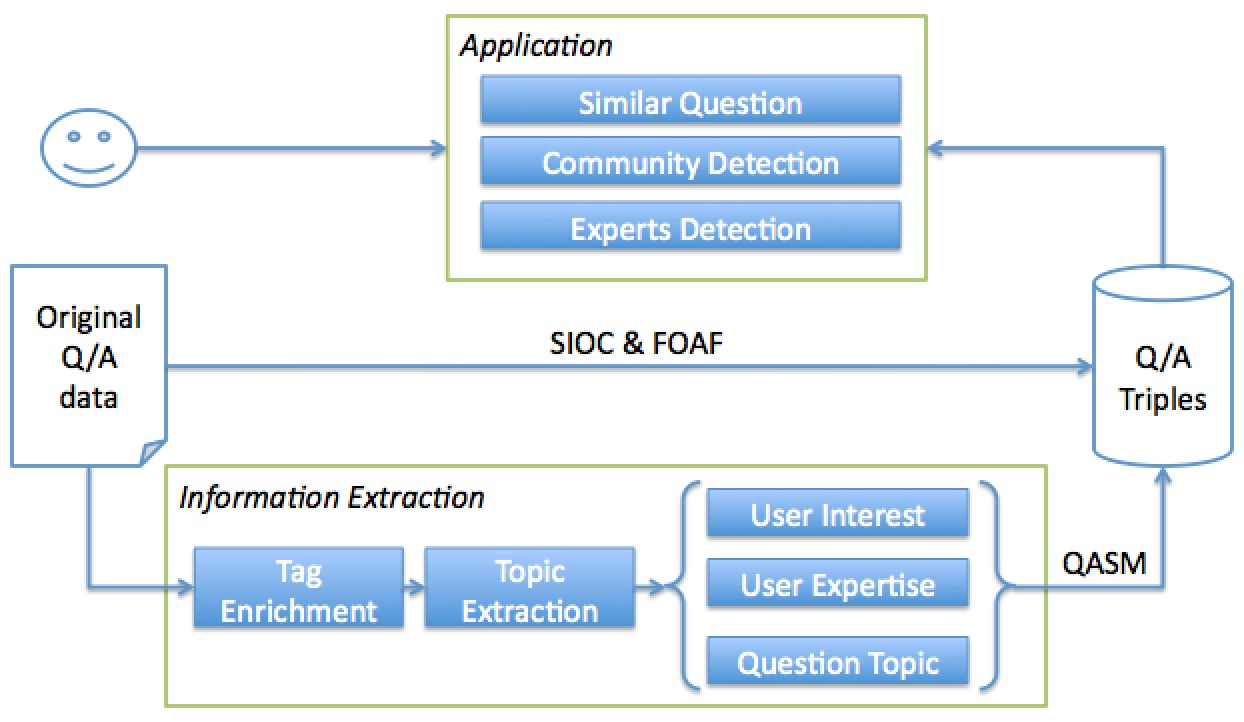
\includegraphics[height=1.857in, width=3.2in]{overview.png}  
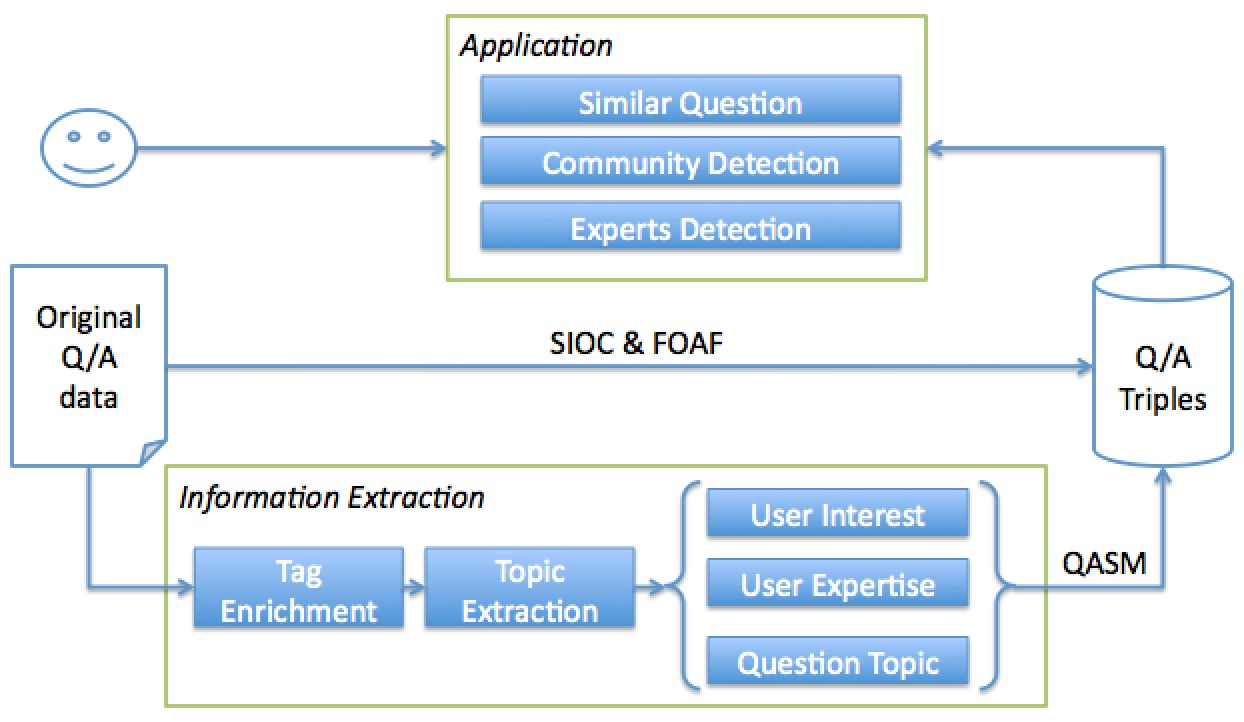
\includegraphics[width=3.2in]{overview.png}  
\caption{Overview of QASM}
\label{fig:overview} 
\end{figure}

\subsection{QASM Vocabulary: formalize Q\&A information}
\begin{figure}[htbp]
\centering
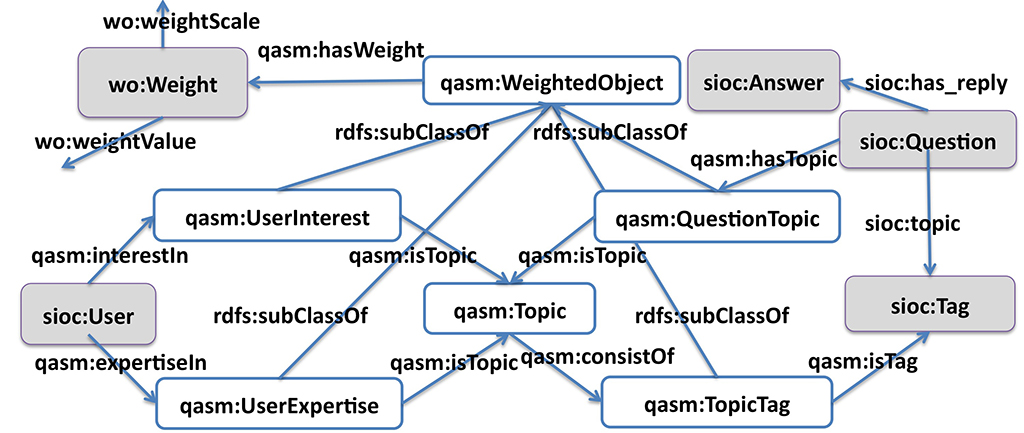
\includegraphics[width=3.7in]{ontologyv2.jpg}  
\caption{Overview of the QASM vocabulary}
\label{fig:coreontology} 
\end{figure}

From the overview, there are mainly two kinds of information that we should formalize. Part of them are explicit, which is the original user-generated content, such as Q\&A contents, user profile, votes, and timestamps. Part of them are implicit, which is detected by social media mining techniques, such as user interest, overlapping communities, user expertise, user activities. 

Existing work focus more on how to formalize the explicit part. We are focusing on extending existing work by formalizing the implicit part. Thus, we proposed QASM vocabulary.  Figure \ref{fig:coreontology} provides an overview of our ontology. It reuses both the SIOC ontology and the Weighting ontology\footnote{http://smiy.sourceforge.net/wo/spec/weightingontology.html}.
The QASM vocabulary\footnote{It is available online at http://ns.inria.fr/qasm/qasm.html} enables to model both explicit and implicit information from Q\&A sites. Table \ref{tab:qaontoclass}shows the main classes used in our work.


\begin{sidewaystable}
    \centering
    \begin{tabular}{c|c|c|c}
    \hline
    Class &  Description & type & onto \\ \hline
    User  & active user & explicit &  sioc:User \\ \hline
    Question & questions post & explicit & sioc:Question \\ \hline
    Answer  & answer post & explicit & sioc:Answer \\ \hline
    Tag & tags used to label questions & explicit & sioc:Tag \\ \hline
    Word & words used in Q\&A content & explicit & qasm:Word \\ \hline
    Topic & bag of words/tags & implicit & QASM:Topic \\ \hline     
    UserInterest& User interest over topic distribution & implicit& qasm:UserInterest\\ \hline
    UserExpertise & User expertise over topic distribution &implicit& qasm:UserExpertise \\ \hline
    TopicTag &Topic over tags distribution&implicit &qasm:TopicTag \\ \hline
    TopicWord&Topic over words distribution &implicit & qasm:TopicWrod\\ \hline
    UserActivity&Topic over users distribution & implicit &qasm:UserActivity \\ \hline
    TopicTrend &Topic over time distribution &implicit & qasm:TopicTrend\\ \hline
          
    \end{tabular}
    \caption{Main Vocabulary (class) used in our work}
    \label{tab:qaontoclass}
\end{sidewaystable}


\begin{sidewaystable}
    \centering
    \begin{tabular}{c|c|c|c|}
    \hline
        Property &  Description & from & to  \\ 
    \hline
    qasm:interestIn  & a user is interested in a topic & sioc:User &  qasm:UserInterest \\ \hline
    qasm:isTopic     & a userInterest object associate with a topic &qasm:UserInterest  &qasm:Topic \\ \hline
    qasm:hasWeight   & a userInterest object associate with a weight&qasm:UserInterest  &wo:Weight \\ \hline
    
    qasm:expertiseIn & a user has expertise in a topic & sioc:User & qasm:UserExpertise \\ \hline
    qasm:isTopic     & a userExpertise object associate with a topic &qasm:UserExpertise &qasm:Topic \\ \hline
    qasm:hasWeight   & a userExpertise object associate with a weight &qasm:UserExpertise &wo:Weight \\ \hline
    
    qasm:consistOf   & a topic is consist of tags   &qasm:Topic &qasm:TopicTag \\ \hline
    qasm:isTag     & a topic tag object associate with a tag  &qasm:TopicTag &sioc:Tag \\ \hline
    qasm:hasWeight   & a topic tag object associate with a weight &qasm:TopicTag &wo:Weight \\ \hline
    
    qasm:consistOf   & a topic is consist of words  &qasm:Topic &sioc:TopicWord \\ \hline
    qasm:isWord     & a topic word object associate with a word  &qasm:TopicWord &sioc:Word \\ \hline
    qasm:hasWeight   & a topic word object associate with a weight &qasm:TopicTag &wo:Weight \\ \hline
    
    qasm:topicTrend  & a topic is popular at a time point & qasm:Topic &  qasm:TopicYearTrend \\ \hline
    qasm:isYear     & a topic trend object associate with a time point &qasm:TopicYearTrend  &qasm:Year \\ \hline
    qasm:hasWeight   & a topic trend object associate with a weight&qasm:TopicYearTrend  &wo:Weight \\ \hline

          
    \end{tabular}
    \caption{Main Vocabulary (property) used in our work}
    \label{tab:qaontoproper}
\end{sidewaystable}

Table \ref{tab:qaontoproper} shows several proprieties used in our work. Since our work mainly generate distributions, we use the same patter to formalize these distributions. As an example, we show an example of formalizing a distribution in Figure \ref{fig:chp3ontoexample}. 

\begin{figure}%[htbp]
\centering
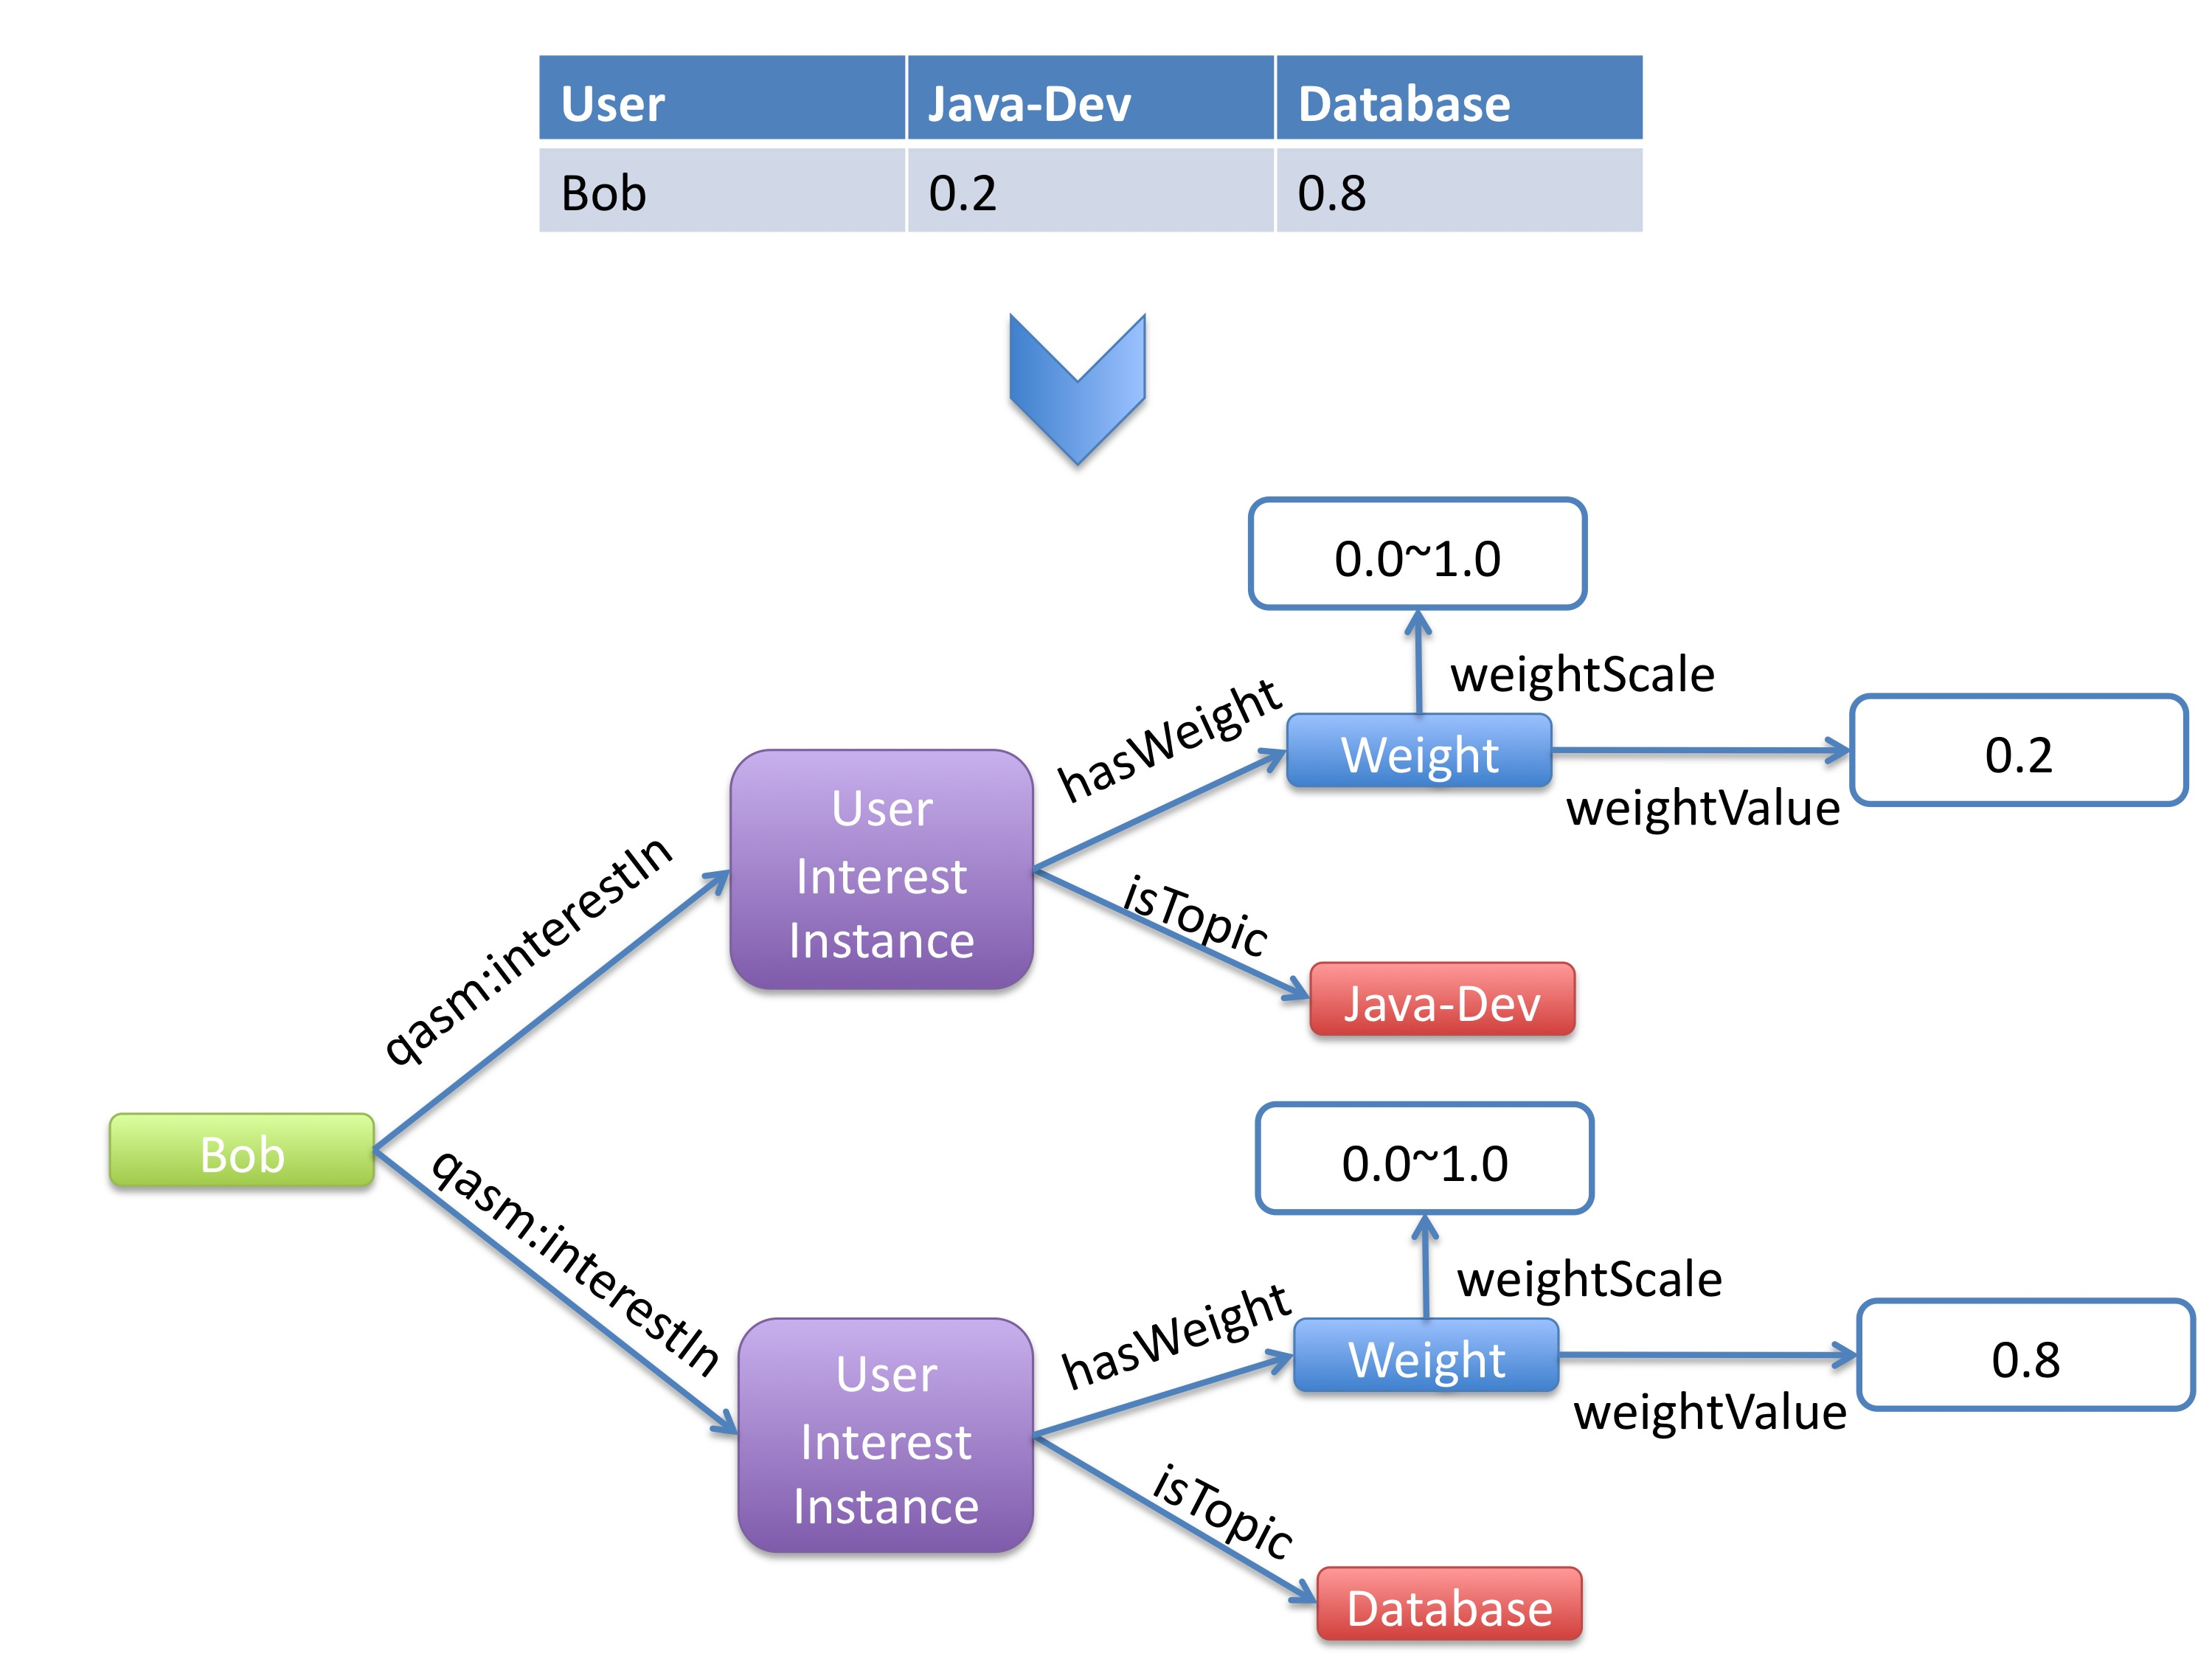
\includegraphics[width=3.2in]{chp3ontoExample.jpg}  
\caption{An example of formalize a distribution}
\label{fig:chp3ontoexample} 
\end{figure}

We explain some core classes and properties as below.

\begin{itemize}
\item \texttt{qasm:Topic} represents a set of tags/words related to a specified topic.
In our models, tags/words belong to instances of \texttt{qasm:Topic}, we also consider different tags/words have different weights for each topic.
\item \texttt{qasm:WeightedObject} is used to describe the weight that a specified subject has with regard to a specified object. This class has four subclasses which represent question topics, users' interests, users' expertise and tag topics respectively. In fact, this class is used to model the distributions we extracted from the original data. For example, topic-tag distribution, user-interest distribution.
\item \texttt{qasm:interestIn} is used to describe the user-interest distribution. This property is different from \texttt{foaf:interest} for its range. In FOAF people are interested in documents, while in QASM a user is interested in a topic to a certain degree (a weight).
\item \texttt{qasm:expertiseIn} is used to describe the user-expertise distribution. A user has different weights for different topics.
\end{itemize}


\subsection{Social media mining: extract the latent knowledge}

Topics, interests, expertise, activity, trend are implicit information in the available raw CQA data. We use social media mining techniques to extract this knowledge.
In Chapter \ref{chp:ttd}, we propose a Tag Tree Distribution method to efficiently extract topic from tags while preserving good quality. Besides, in Chapter \ref{chp:ttea}, we jointly model topic, interest, expertise and trend to extract the relations between them, such as user-topic, topic-time, user-expertise, user-interest etc. In addtion, Chapter \ref{chp:label} propose a method by using DBpedia to generate label for a bag of words which is used to define a topic. 
We list all the latent knowledge extracted by our models and explain them one by one.




\textbf{Topic}: A bag of words or tags which are closely related. Words are the content of questions or answers, tags are attached to questions. For example, the topic-tag distribution \textit{Database}:\{{\textit{mysql}: 0.5, \textit{sql}: 0.3, \textit{query}: 0.2\}. expresses that topic \textit{Database} is related to tags \textit{mysql}, \textit{sql}, and \textit{query}. 


\textbf{User Topical Interest}: A user is interested in different topics with different levels. For example, the user-topic distribution \textit{Alice}:\{{\textit{Database}: 0.8, \textit{Java}: 0.2\} expresses that \textit{Alice} prefers to answer questions related to \textit{Database}, but rather not about \textit{Java}. 

\textbf{User Topical Activity}:  Different users are interested in the same topic with different levels. For example, the topic-user distribution \textit{Database}:\{{\textit{Alice}: 0.8, \textit{Bob}: 0.2\} expresses that \textit{Alice} prefers to answer question related to \textit{Database}, while \textit{Bob} is not willing to contribute answers to it.

\textbf{Topic Trend}: A topic is popular at different points in time with different levels. For example,the topic-time distribution \textit{Database}:\{{\textit{May/2013}: 0.2, \textit{June/2013}: 0.3, \textit{July/2013}: 0.5\} expresses that the topic \textit{Database} is increasingly popular.% while the topic \textit{java} remains stable.

\textbf{Topic Temporal Activity}: Topics are active at a point in time with different levels. For example, the time-topic distribution \textit{Sept/2013}:\{{\textit{Ios}: 0.8, \textit{Database}: 0.2\} expresses that \textit{ios} related questions are popular in Sept. 2013, while \textit{Database} related questions are not specially popular.

\textbf{User Topic Temporal Dynamics}: A user is interested in different topics at different points in time with different levels. For example, the topic-time distribution for \textit{Alice} \textit{ios}:\{{\textit{May/2013}: 0.2, \textit{June/2013}: 0.3, \textit{July/2013}: 0.5\} expresses that \textit{Alice}'s interest to topic \textit{ios} is increasing.


\textbf{User Topical Expertise}: A user has expertise in different topics with different levels. For example, the topic-expertise distribution for \textit{Alice} \textit{ios}:\{{\textit{High}: 0.2, \textit{Medium}: 0.7, \textit{Low}: 0.1\} expresses that \textit{Alice}'s expertise on topic \textit{ios} is probably in medium level.



\section{Summary: an effective way to manage q\&a sites}
\label{sec:future}
We presented QASM, a Q\&A system combining social media mining and semantic web models and technologies to manage Q\&A users and content in CQA sites. This chapter provide us a framework to manage user-generated content and extracted latent knowledge on Q\&A sites. In the next chapters, we will focus on how to efficiently extract these latent knowledge, such as topics and communities. And how to extract more latent information such as topic based temporal dynamics, topic based expertise.







\chapter{Adapting Latent Dirichlet Allocation to Overlapping Community Detection}
\doublespacing
\label{chap:lda}
\minitoc

\section{Introduction to the Latent Dirichlet Allocation Adaptation}
In Natural Language Processing (NLP), Latent Dirichlet Allocation (LDA) \cite{blei2003latent} is a classical document clustering method, a Bayesian network that models how documents in a corpus are topically related.
It is used to detect latent topics from documents by constructing a three-layer probabilistic graphical model: document-topic-word. In this three-layer model, documents and words can be observed from a dataset, while topics are a hidden layer which has to be estimated from the observed data.  
In StackOverflow, a user submits a question, then assigns 1$\sim$5 tags to indicate the key topics touched by this question. Other users who are interested in the question may provide answers to the question or comment on the question or others' answers. Therefore the main structuring graph in StackOverflow is the question-answer graph. As tags attached to a question  reflect its scope and domain, users answering a question can be considered as interested by this domain. As a result, a first approach is to consider that a user answering a question acquires the tags attached to this question and gradually, each user acquires a list of tags associated with frequencies. If we treat a user as a document and tags acquired by the user as words in a document, then community detection can be considered as a clustering problem where users with similar topics of interest are grouped into the same cluster forming a community of interest.

Similarly to \cite{Li:2010:CTM:1871437.1871673}, we applied the classic LDA method to construct a users-topics-tags model to detect latent topics of interest from the tags acquired by users and then cluster users into different topics. The output of the model consists of two probability distributions:
\begin{enumerate}
 \item a User-Topic distribution to describe to what extent a user is interested in the different topics.
 \item a Topic-Tag distribution to describe to what extent a topic is related the different tags.
\end{enumerate}



The formalization of this model is given by equation~\ref{eq:general}: 
\begin{equation}
P(t|u)=P(t|z)*P(z|u)
\label{eq:general}
\end{equation}
where $t$ denotes a tag, $z$ denotes a latent topic, $u$ denotes a user. The probability of a tag for a user is the result of multiplying the probability of this tag for a topic and the probability of this topic for the user.

%TODO: Fab: I changed the text below please check it is correct
Probabilistic graphical models (PGM) express the conditional dependence structure between random variables as a graph. 
The plate notation of the PGM of our model is presented in Figure \ref{fig:lda}. 
The variables appear as blue disks if the variable is observed and white disks if the variable is hidden (guessed).
The dependencies among the variables are captured by the direction of the edges. 
The boxes represent replicated variables, which are users, topics (interests) and tags. The outer boxes represent users, while the inner boxes represent the repeated choice of topics and tags for a user. The parameters of this model are explained in Table \ref{tab:parameters}.
$M$ and $V$ are given while $K$, $\alpha$ and $\beta$ can be chosen. $T$ is observed through the users' tag lists. Other variables are latent variables which have to be estimated.

\begin{figure}[htbp]\centering
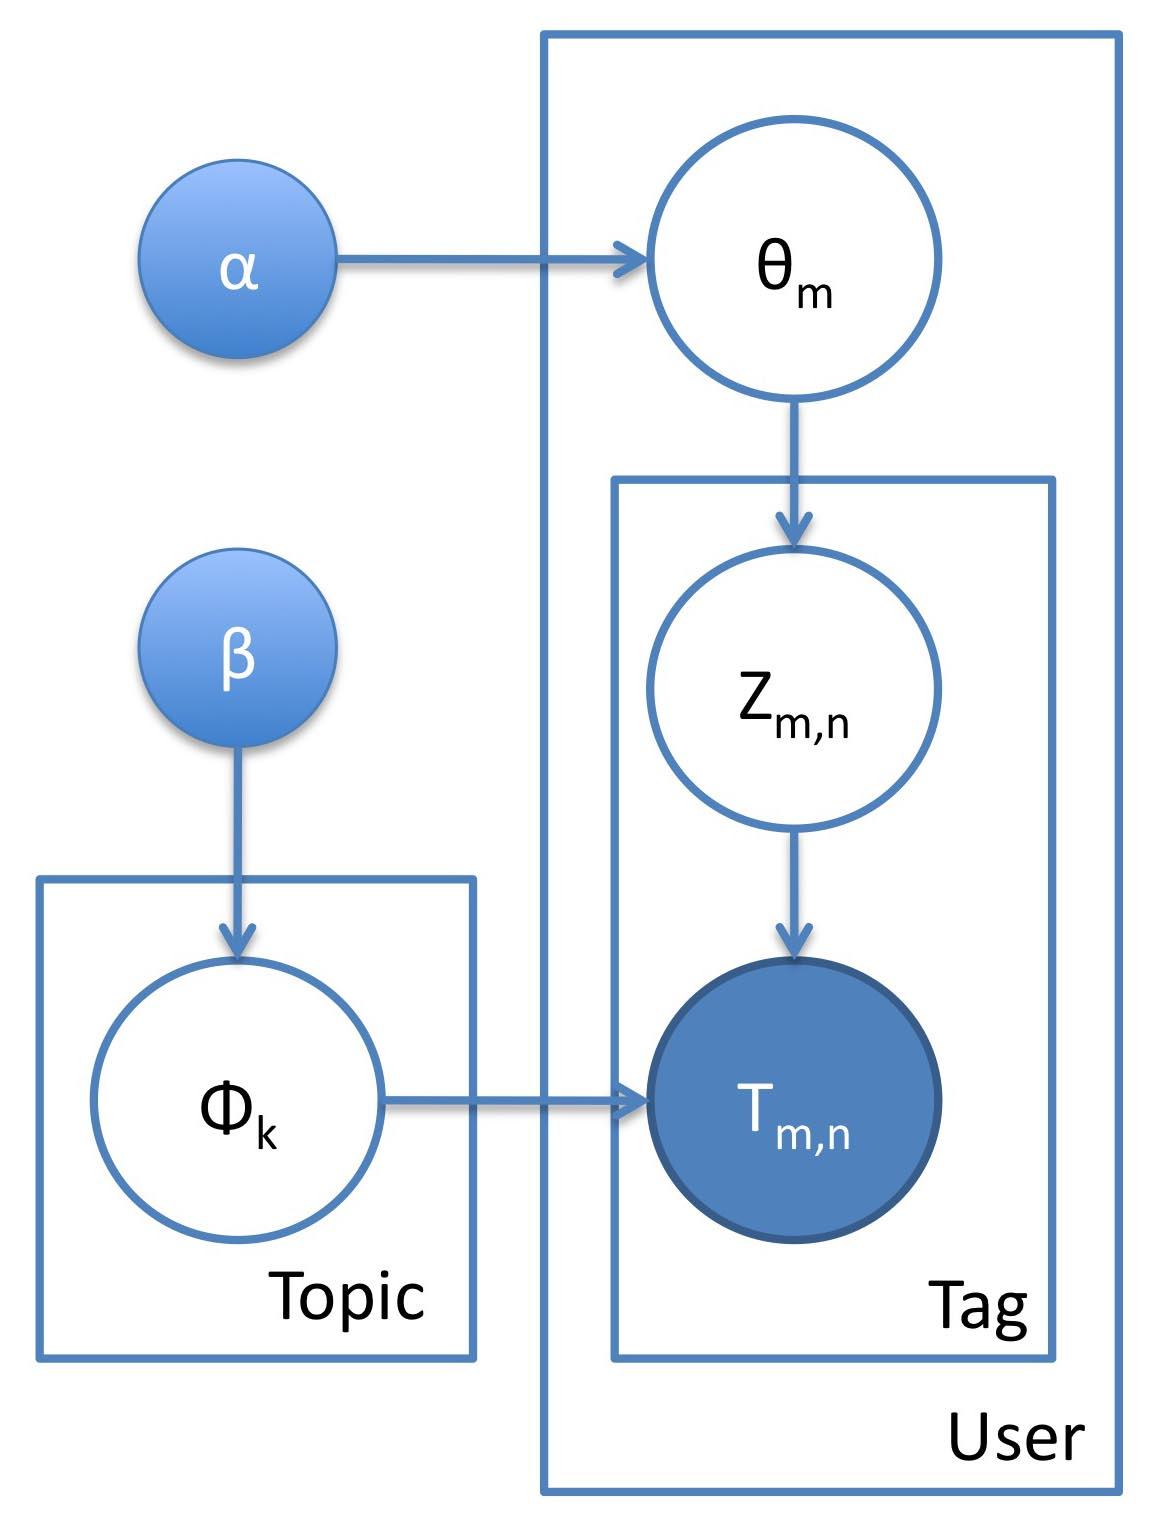
\includegraphics[ width=3.0in]{lda.jpg}  % "pdflatex"
\caption{User-Topic-Tag (LDA) Model}
\label{fig:lda}
\end{figure}

The intuition behind this model is that users choose their topics and that these chosen topics drive the generation of the tags.
The generative process can be summarized as follows:

%TODO : reformat process as code / pseudo algorithm style
\noindent\rule[0.5ex]{\linewidth}{1pt}
\textbf{Process of generating a user's tag list}\\
\noindent \textbf{for} interest k \textbf{in} [1..K]:\\
\indent draw topic tag distribution $\phi(k)$ $\sim$ Dir($\beta$)\\
\noindent \textbf{for} user $m \in [1,M]$:\\
\indent draw a user-topic distribution $\theta(m)$ $\sim$ Dir($\alpha$)\\  
\indent \textbf{for} each tag $n \in$   user $m$'s tag list, where $n~\in~[1,N_m]$, $m~\in~[1..M]$\\
\indent \indent draw topic $z_{m,n}$  $\sim$ Multi($\theta(m)$)\\
\indent \indent draw tag $t_{m,n}$ $\sim$ Multi($\phi(z_{m,n})$)\\ 
\noindent\rule[0.5ex]{\linewidth}{1pt}

\begin{table}[htbp]
\caption{Model parameters}
\label{tab:parameters}
\centering
\begin{tabular}{|c|c|}
\hline
Parameter & Meaning \\
\hline
$M$ & the total number of users\\
\hline
$K$ & the total number of topics\\
\hline
$V$ & the total number of tags\\
\hline
$N_m$ & the total number of tags for user $m$\\
\hline
$\alpha$ & the parameter of the Dirichlet prior on the per-user topic distributions \\
\hline
$\beta$ & the parameter of the Dirichlet prior on the per-topic tag distributions  \\
\hline
$\theta_m$ & the topic distribution for user $m$ \\
\hline
$\phi_k$ & the tag distribution for topic $k$ \\
\hline
$z_{m,n}$ & the topic for $n^{th}$ tag in $m$'s tag list \\
\hline
$t_{m,n}$ & the specified tag in $n^{th}$ position of $m$'s tag list\\
\hline

\end{tabular}
\end{table}

We use the collapsed Gibbs Sampling method~\cite{griffiths2004finding} to sample the hidden variable $z$, then $\theta$ and $\phi$ can both be estimated.
The inference process is as follows.
We iteratively sample the topic indicator $z_{m,n}$ for each answer tag $t_{m,n}$ according to equation \ref{eq:ldasample}. 


\begin{equation}
\begin{split}
p(z_i= z_{m,n} |u=u_m, t=t_{m,n}, Z, U, T_{\neg i}) &\\
\propto \frac{ C_{u_m,\neg i}^{z_{m,n}} + \alpha }{ \sum_{k=1}^K C_{u_m,\neg i}^k + K* \alpha} &\\
\cdot   \frac{ C_{z_{m,n},\neg i}^{t_{m,n}} + \beta }{ \sum_{t=1}^V C_{z_{m,n},\neg i}^t + V* \beta} &\\ 
\end{split}
\label{eq:ldasample}
\end{equation}

\noindent
where $\neg i$ enforces that all the counters used are calculated with tag $t_i$ excluded. $C_{u,\neg i}^k$ is the number of tags acquired by user $u$ assigned to topic $k$, $C_{k,\neg i}^{t}$ is the number of tags $t$ assigned to topic $k$.

Then with a Gibbs sampling, we can estimate $\theta$ and $\phi$ by equation \ref{eq:computetheta} and \ref{eq:computephi}:

\begin{equation}\scriptsize
\theta=\frac{ C_u^k + \alpha}{ \sum_{k=1}^K C_u^k+ K* \alpha}
\label{eq:computetheta} 
\end{equation}
\begin{equation}\scriptsize
\phi =\frac{ C_k^t + \beta}{ \sum_{t=1}^V C_k^t+ V* \beta}
\label{eq:computephi} 
\end{equation}

\noindent
where $C_u^k$ is the number of tags assigned to topic $k$ of user $u$ , $C_k^t$ is the number of tags $t$ assigned to topic $k$.


\section{First experiments: find topics and communities with adapted LDA}
%TODO: FAB: here we are missing details on (1) the dataset characteristics - the dataset of your PhD must be described either at the begining and reference with a unique identifier and reference to the description section if they are used in several chapters OR before the experiment where they are used if they are used only once (2) the implementations, languages, libaries, etc. you used to perform the experiment.

We ran the above described model on a dataset from the popular Q\&A site StackOverflow, each user being represented by her tag list as explained before. We just illustrate some of the results to show the effectiveness of this model.

A first result is the probability for each tag to belong to each topic. This is  shown in Table \ref{tab:ldaresult1}. 
The second result is the probability for a user to belong to different topics of interest. This is shown in Table \ref{tab:ldaresult2}. 
%TODO: FAB: you can add graphical views of these data.

Table \ref{tab:ldaresult1} shows eight examples of the detected topics of interest, each column showing one topic, and the ten rows giving the top 10 tags for each topic, sorted by descending weights. The weight of a tag is the probability of the tag to belong to the topic.  
This table shows that each topic has a clear and focused interest. For example, topic 1 has c-development related tags, topic 2 has java-development related tags, topic 3 has c\#-development related tags, topic 4 has html-development related tags, topic 5 has iphone-development related tags, topic 6 has database related tags, topic 7 has linux-development related tags, topic 8 has non-programming related tags. 
Moreover, weights reflect the relevance of tags to each topic. For example, topic 5 is concerned with iphone-development and its top 3 tags are 'iphone', 'objective-c' and 'cocoa' which are indeed very relevant.
\begin{sidewaystable}
\centering
%\begin{tabular}{|p{40pt}||p{40pt}||p{40pt}||p{40pt}|}
\begin{tabular}{|l|l|l|l|}
\hline
\textbf{topic1} & \textbf{topic2} & \textbf{topic3} & \textbf{topic4} \\
\hline
%\multicolumn{4}{|c|}{c++(0.225), c(0.084), java(0.345), java(0.345), java(0.345), java(0.345), java(0.345), java(0.345), java(0.345), java(0.345)}\\
%\hline
 \textbf{c++}(0.225)& \textbf{java}(0.345)& \textbf{c\#}(0.225)& \textbf{php}(0.117) \\ 
\hline
 \textbf{c}(0.084)& \textbf{eclipse}(0.023)& \textbf{.net}(0.128)& \textbf{javascript}(0.115) \\ 
\hline
 \textbf{windows}(0.020)& \textbf{swing}(0.015)& \textbf{asp.net}(0.059)& \textbf{html}(0.059) \\ 
\hline
 \textbf{stl}(0.014)& best-practices (0.014)& \textbf{vb.net}(0.019)& \textbf{jquery}(0.056) \\ 
\hline
 algorithm(0.014)& multithreading (0.011)& \textbf{linq}(0.018)& \textbf{css}(0.042) \\ 
\hline
 c\#(0.013)& xml(0.010)& windows-forms (0.016)& mysql(0.029) \\ 
\hline
 \textbf{win32}(0.013)& \textbf{spring}(0.010)& \textbf{visual-studio} (0.015)& \textbf{ajax}(0.021) \\ 
\hline
 linux(0.011)& performance (0.009)& \textbf{asp.net-mvc} (0.015)& \textbf{web-development} (0.019) \\ 
\hline
 best-practices (0.011)& jsp(0.008)& wpf(0.012)& regex(0.018) \\ 
\hline
 multithreading (0.011)& generics(0.008)& best-practices (0.011)& \textbf{asp.net}(0.015) \\ 
\hline
\hline
\textbf{topic5} & \textbf{topic6} & \textbf{topic7} & \textbf{topic8} \\
\hline
 \textbf{iphone}(0.137)& \textbf{sql}(0.181)& \textbf{python}(0.181)& subjective(0.143) \\ 
\hline
 \textbf{objective-c} (0.123)& \textbf{sql-server}(0.150)& \textbf{perl}(0.056)& \textbf{best-practices} (0.038) \\ 
\hline
 \textbf{cocoa}(0.080)& \textbf{database}(0.062)& \textbf{regex}(0.031)& \textbf{language-agnostic} (0.035) \\ 
\hline
 ms-access(0.062)& delphi(0.042)& \textbf{linux}(0.030)& programming (0.028) \\ 
\hline
 \textbf{cocoa-touch} (0.056)& \textbf{sql-server-2005} (0.042)& \textbf{ruby}(0.027)& \textbf{not-programming-related} (0.019) \\ 
\hline
 \textbf{iphone-sdk} (0.041)& \textbf{mysql}(0.039)& django(0.023)& \textbf{career-development} (0.018) \\ 
\hline
 vba(0.035)& \textbf{tsql}(0.037)& ruby-on-rails (0.021)& \textbf{learning}(0.017) \\ 
\hline
 excel(0.023)& \textbf{oracle}(0.028)& beginner(0.017)& polls(0.017) \\ 
\hline
 vb6(0.022)& \textbf{database-design} (0.025)& git(0.013)& programming-languages (0.015) \\ 
\hline
 xslt(0.021)& \textbf{stored-procedures} (0.017)& \textbf{bash}(0.013)& \textbf{design}(0.014) \\ 
\hline
\end{tabular}
\caption{Top 10 related tags for detected topics of interest}
\label{tab:ldaresult1}
\end{sidewaystable}

Table \ref{tab:ldaresult2} shows six randomly chosen users and their top 10 tags. The first row contains user ids, the second row contains their detected topics of interest with their probability. The following ten rows show the top 10 tags for each user. We replaced topic ids with topic names which we have assigned to them according to their associated tags.
\begin{sidewaystable}%[htbp]
\centering
%\begin{tabular}{|p{60pt}|p{60pt}|p{60pt}|}
\begin{tabular}{l|l|l}
\hline
user\_21886&user\_14860&user\_15401\\
\hline
\textbf{\textcolor{blue}{html-development}} (0.284)  & \textbf{\textcolor{blue}{c-development}} (0.333) &\textbf{\textcolor{blue}{database-related}} (0.383)\\
 \textbf{\textcolor{brown}{c-development}} (0.275) &  \textbf{\textcolor{brown}{linux-development}} (0.196)& \textbf{\textcolor{brown}{non-programming-related}} (0.290)\\

\hline
python(93)&\textcolor{blue}{c}(152)&\textcolor{blue}{sql-server}(108)\\
%\hline
\textcolor{brown}{c++}(64)&\textcolor{blue}{c++}(148)&\textcolor{blue}{database}(64)\\
%\hline
\textcolor{blue}{javascript}(45)&java(89)&\textcolor{blue}{sql}(63)\\
%\hline
\textcolor{blue}{html}(34)&subjective(89)&\textcolor{brown}{subjective}(45)\\
%\hline
\textcolor{brown}{c\#}(33)&c\#(68)&python(43)\\
%\hline
\textcolor{blue}{css}(32)&sql(68)&\textcolor{blue}{sql-server-2005}(31)\\
%\hline
\textcolor{brown}{visual-studio}(29)&\textcolor{blue}{windows}(67)&\textcolor{brown}{best-practices}(27)\\
%\hline
\textcolor{brown}{windows}(27)&\textcolor{brown}{linux}(54)&.net(25)\\
%\hline
\textcolor{brown}{c}(27)&\textcolor{brown}{bash}(48)&c++(23)\\
%\hline
.net(24)&\textcolor{brown}{regex}(43)&c\#(22)\\
\hline
\hline
user\_78374&user\_53897&user\_23743\\
\hline
\textbf{\textcolor{blue}{non-programming-related}} (0.493)&\textbf{\textcolor{blue}{java-development}} (0.835)&\textbf{\textcolor{blue}{iphone-development}} (0.683)\\
\textbf{\textcolor{brown}{linux-development}} (0.316)&\textbf{\textcolor{brown}{non-programming-related}} (0.075)& \textbf{\textcolor{brown}{non-programming-related}} (0.155)\\

\hline
\textcolor{blue}{subjective}(35)&\textcolor{blue}{java}(366)&\textcolor{blue}{objective-c}(73)\\
%\hline
\textcolor{brown}{python}(32)&\textcolor{blue}{eclipse}(24)&\textcolor{blue}{cocoa}(71)\\
%\hline
\textcolor{blue}{best-practices}(16)&\textcolor{blue}{tomcat}(20)&\textcolor{blue}{iphone}(34)\\
%\hline
c(13)&\textcolor{brown}{subjective}(18)&\textcolor{blue}{cocoa-touch}(21)\\
%\hline
programming(13)&\textcolor{blue}{performance}(18)&\textcolor{blue}{mac}(19)\\
%\hline
c++(10)&\textcolor{brown}{best-practices}(16)&\textcolor{blue}{osx}(17)\\
%\hline
\textcolor{blue}{beginner}(8)&\textcolor{blue}{j2ee}(14)&\textcolor{blue}{iphone-sdk}(13)\\
%\hline
\textcolor{blue}{not-programming-related}(8)&\textcolor{blue}{jar}(13)&\textcolor{blue}{xcode}(10)\\
%\hline
\textcolor{blue}{language-agnostic}(6)&logging(10)&\textcolor{brown}{subjective}(8)\\
%\hline
\textcolor{blue}{coding-style}(5)&c\#(9)&c(8)\\
\hline
\end{tabular}
\caption{Detected topics of interest}
\label{tab:ldaresult2}
\end{sidewaystable}

\section{Discussion: the limitation and problems}
The above experiments verified that, by applying topic models on Q\&A website, we are ideed able to detect overlapping communities, and that the detected topics are meaningful and could be used to explain the shared interest of each corresponding community as in our work, we directly use each topic to represent a community of interest.

However, we found that there are three limitations when applying LDA models to our task:

\begin{itemize}
  \item The first one is a lack of efficiency: the complexity of the probabilistic model was prohibitive.
  %TODO: FAB you should provide details on the computation time, complexity, etc. to make your point
  \item The second limitation is that the  original LDA model does not enable to extract temporal and expertise information. 
  %TODO: FAB explain why i.e. what is missing in the model to achieve that
  \item The third limitation is that the detected probability distributions cannot be compared with each other.
  %TODO: FAB explain why i.e. what noramilization would be required to do that AND why this would be useful
\end{itemize}

Therefore, in the rest of this thesis we extended our work in two directions:

\begin{enumerate}
 \item First, we developed a more simple method to detect topics and overlapping communities to solve the first problem: the TTD method is presented in Chapter \ref{chap:ttd}.
  \item Second, we propose a more complex model to extract more information from user generated content to answer the two other limitations: the TTEA method is presented in Chapter \ref{chap:ttea}.
\end{enumerate}
 


\chapter{Topic Extraction: identifying topics from tags}
\doublespacing
\label{chap:ttd}
\minitoc

\section{Topic Trees Distributions (TTD)}\label{sec:TTD}
\label{sec:empirical}

\subsection{Problem Definition: mining topics and communities}
% TODO: add a paragraph explaininh the link with previous chapter and itroducing the need for this new chapter e.g. classical LDA is too slow.
%DONE
In Chapter \ref{chap:qasm}, we mentioned that there are two kinds of information in user-generated content. One of them is latent information such as topics and communities, which are not explicitly existed in the original data set. In this chapter, we aim at extracting these latent information from tags on Q\&A sites.

In Chapter \ref{chap:lda}, we applied the original LDA model and we found it is complicated and slow to extract these latent information. In this chapter, we aim at proposing a much simple and efficient method to extract these information. 

% TODO: do not repeat what was said in prvious chapter e.g. the definitions should be given once in the whole thesis.
% TODO: the previous TODOs applay to all chapters
Many sites supporting user-generated content let their members organize their contributions with tags. The social tagging approach also applies to Q\&A platforms. In particular, in StackOverflow, a user submits a question, then assigns 1$\sim$5 tags to indicate the topics of the question. Other users who are interested in the question may provide answers to the question. As the tags attached to a question can reflect its topic, users asking the question can be considered as interested by its topic and users successfully answering a question can be considered as experts in that topic.

Let $U=\{u_1,u_2...u_n\}$ be the set of users, $Q=\{q_1,q_2...q_m\}$ the set of questions and $T=\{t_1,t_2...t_v\}$ the set of tags. We aim at:

\begin{enumerate}
 \item extracting topics distribution $Topic=\{topic_1,topic_2...topic_k\}$ from $T$, and for each $topic_k$, defining $topic_k=\{p_{k1},p_{k2}...p_{kv}\}$ where $p_{ki}$ denotes the probability of tag $t_i$ to be related to $topic_k$; an then
  \item detecting user's interests. For a user $u_i \in U$, we define $I_i=\{I_{i1},I_{i2}...I_{ik}\}$ where $I_{ik}$ denotes the probability of $u_i$ to be interested in $topic_k$.
\end{enumerate}


\subsection{First-Tag Enrichment: adding a more general tag when needed}
When sorting the tags of a question by their global frequency, we found that normally the first tag of a question is much more general and indicates the domain of the question. For example, a question tagged with \{\textit{c\#}, \textit{iostream}, \textit{fstream}\} is related to \textit{c\#}; a question tagged with \{\textit{html}, \textit{css}, \textit{height}\} is related to \textit{html}. However, there are also some questions which have less tags and, in this case, the tags are less popular, like a question tagged with \{\textit{ant}\} or a question tagged with \{\textit{qt}, \textit{boost}\}. For these questions, the main domain is implicit. Our experiment dataset shows that nearly $12\%$ of the questions only have one tag, and nearly $25\%$ of the questions only have two tags.

% TODO: justify the heuristics, do you have the metrics we talked about eg correlation between frequency and rank ?    


Therefore, we propose an approach to enrich a question with a first tag when needed. The first step of our approach consists in computing the first-tag distribution.
\begin{figure}[htp]
\centering
%\epsfig{file=fly.eps, height=1in, width=1in} % use this if you use "pdflatex"
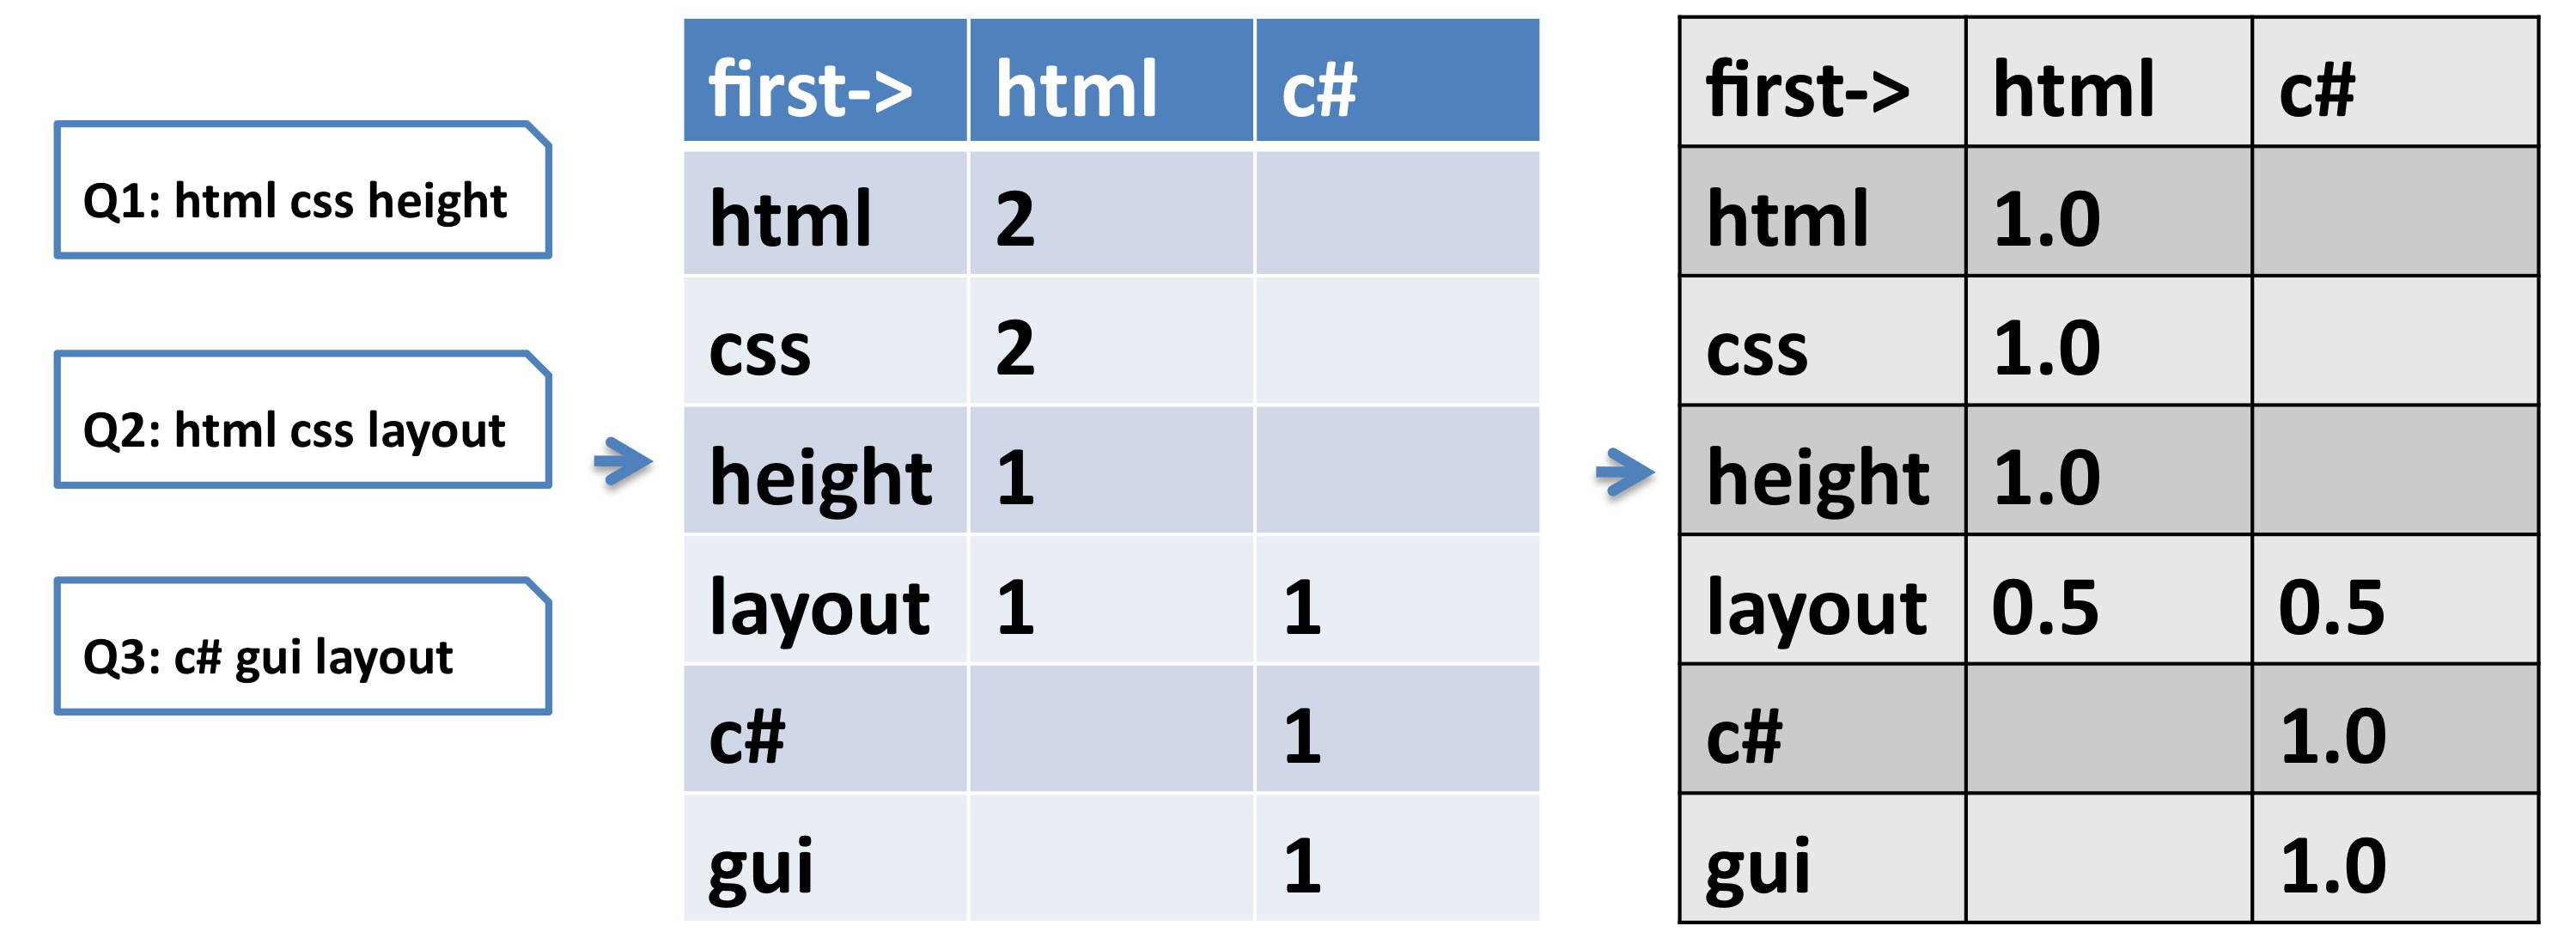
\includegraphics[width=5in]{7.jpg}  
\caption{Example of computing a first-tag distribution}
\label{fig:examplefirsttag} 
\end{figure}
For example, as shown in Figure \ref{fig:examplefirsttag}, let us consider the three tag lists, \{\textit{html}, \textit{css}, \textit{height}\},  \{\textit{html}, \textit{css}, \textit{layout}\}, and \{\textit{c\#}, \textit{gui}, \textit{layout}\}, respectively associated to questions Q1, Q2, Q3 . The first-tag frequency map for \textit{html} is \{\textit{html}:2\}, the first-tag frequency map for \textit{css} is \{\textit{html}:2\}, and the first-tag frequency map for \textit{layout} is \{\textit{html}:1,\textit{c\#}:1\}. Given a tag, the probability of its first-tag is computed by equation \ref{eq:firsttag}, which is the Maximum Likelihood estimation (MLE) of the probability $p(T_f|T_i)$, where $I(T_i)$ denotes the occurrence of tag $T_i$ and $I(T_f,T_i)$ denotes the co-occurrence of first-tag $T_f$ and tag $T_i$.

\begin{equation}
%\scriptsize
\begin{split}
p(T_f|T_i)  &=\frac{p(T_f,T_i) }{p(T_i)} \\
                  &\propto \frac{I(T_f,T_i)}{I(T_i)}
\label{eq:firsttag}
\end{split}
\end{equation}


We compute the probabilities just by normalizing the first-tag frequency map. In the previous example, the first-tag frequency map for \textit{css} becomes \{\textit{html}:1.0\} and the first-tag frequency map for \textit{layout} becomes \{\textit{html}:0.5, \textit{c\#}:0.5\}. In order to lower the probabilities of low frequency tags as first-tag, we use the squashing function \ref{eq:normalize}:

%TODO : you equations should use proper mathematical notation for sums, you should define p(Tf,Ti) and define a frequency function for tags and for tag pairs ; here it is not easy to see over what set you sum
%DONE


\begin{equation}
\begin{split}
p(T_f|T_i) &=\frac{I(T_f,T_i)}{I(T_i)}*\sigma(I(T_f)) \\
                  %&=\frac{record\_freq}{sum(record\_freq)} 
                  &\propto \frac{I(T_f,T_i)}{I(T_i)}*\frac{1}{(1+e^{-k*I(T_f)})}
\label{eq:normalize}
\end{split}
\end{equation}

where, $I(T_f)$ denotes the frequency of \textit{first-tag}. $I(T_f,T_i)$ denotes the co-occurrence of \textit{first-tag} and \textit{tag}, $I(T_i)$ denotes the frequency of \textit{tag}  $\sigma(x)$ is sigmoid function, which is used as a squashing function for numerical stability. The value of sigmoid function is between 0 and 1, however the shape of this function is largely determined by parameter $k$. Considering the maximum value of tag frequency (tag c\#:$31,801$) in our dataset, we chose $k$ as 0.001 (dotted line), which will lower the probabilities of low frequency tags as first-tag while maintaining the probabilities of high frequency tags as first-tag. Figure \ref{fig:sigmoidfunction} recalls the shape of the sigmoid function for different values of $k$.

\begin{figure}[htp]
\centering
%\epsfig{file=fly.eps, height=1in, width=1in} % use this if you use "pdflatex"
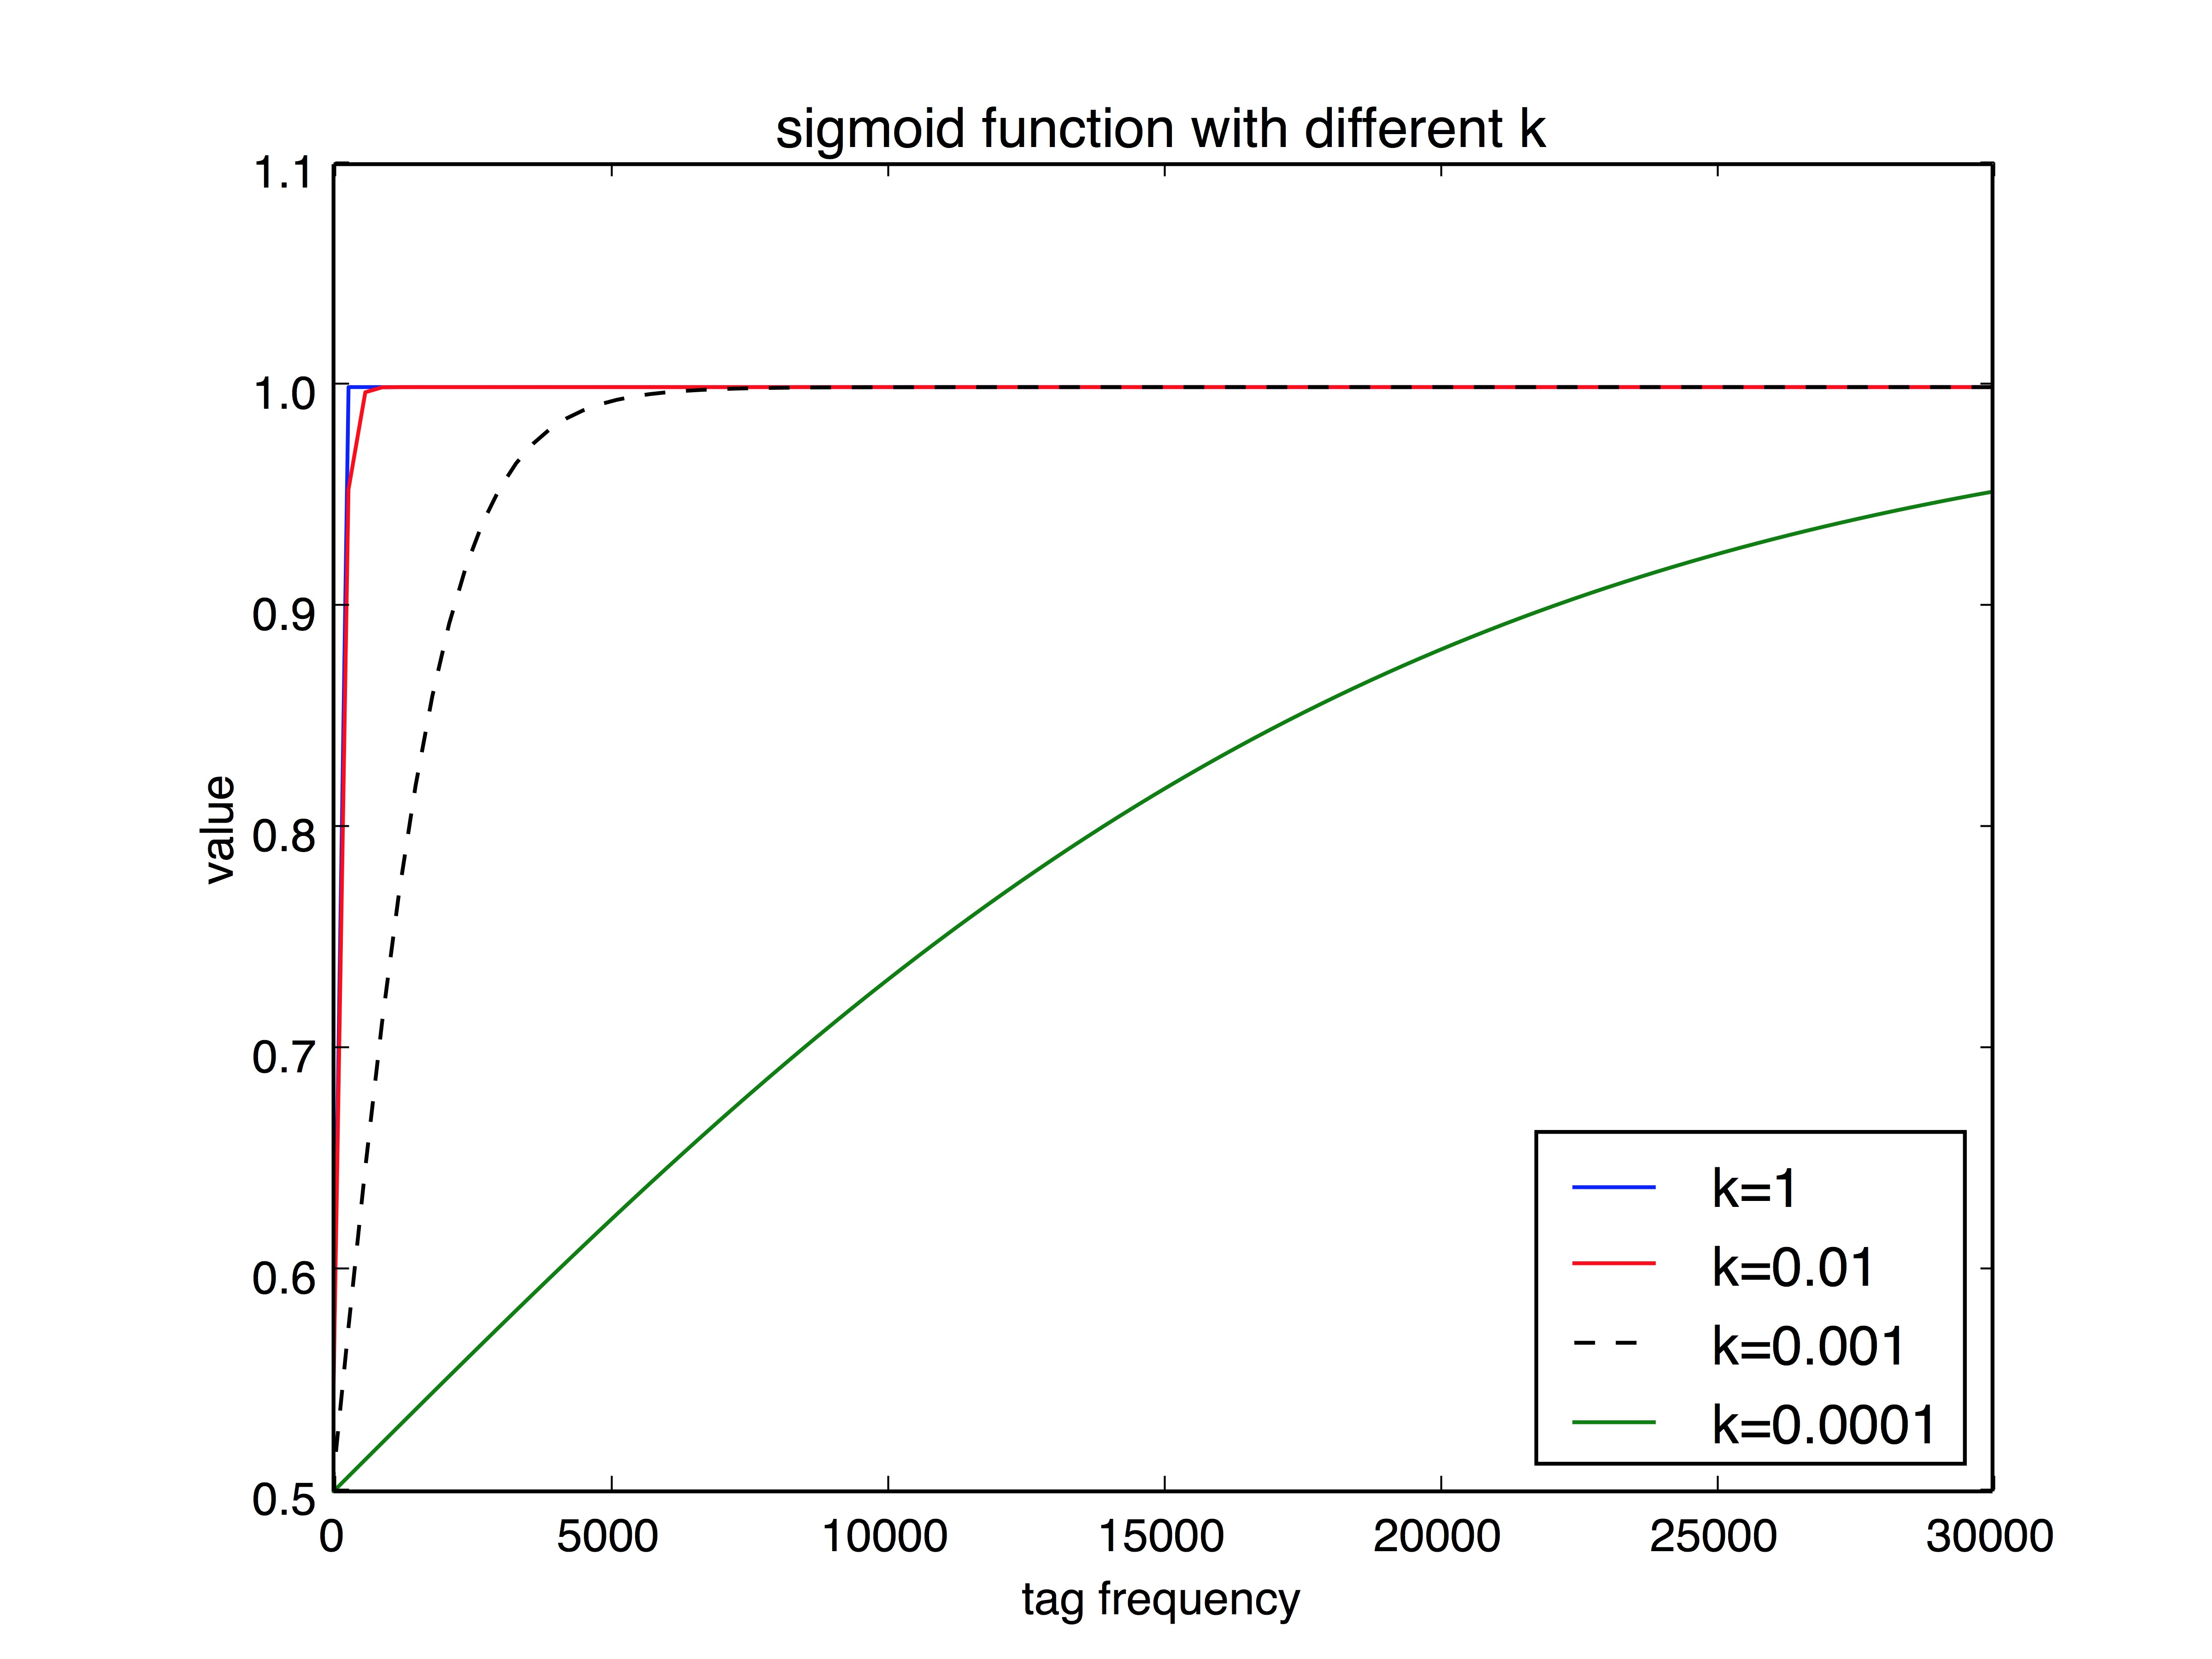
\includegraphics[width=5in]{sigmoid.jpg}  
\caption{Shape of function $\frac{1}{(1+e^{-k*z})}$ for different values of $k$}
\label{fig:sigmoidfunction} 
\end{figure}
For example, if the first-tag frequency map for \textit{css} is \{\textit{html}:10, \textit{jquery}:2\}, then, when normalizing first-tag \textit{html}, $I(T_f,T_i)=10$, $I(T_i)=12$, $I(T_f)=5,552$. As a result, $p(html|css)=0.8301$. 
Similarly, for each tag, we provide a list of candidate first-tags with estimated probabilities. 

The second step of our approach consists in choosing a first-tag to enrich each question. Given a question's tag list, we fetch the top 5 first-tags (with the highest probabilities). Then we accumulate the corresponding probabilities with a discount function taking into account the position of the tag in the tag list associated to the question, as shown in equation \ref{eq:accumulate}: 
\begin{equation}
\begin{split}
 p_{j}=  p_{1,j}+p_{2,j}*dis+...+p_{k,j}*dis^{k-1} \\
\end{split}
\label{eq:accumulate}
\end{equation}

%TODO: you noted there could be two kinds of discount, one is liner discount, another is non-liner, such as log discount. need to prove which is better. 
%DONE
%I put it in the experiment section. 

 %for j \in [1,V], k \in [1,K]
where $p_{j}$ denotes the probability of  tag $j$ to be the first-tag of a given question, $p_{k,j}$ denotes the probability for tag $k$ to have tag $j$ as its first-tag. The range of $v$ and $k$ are $[1,V]$ and $[1,K]$, where $V$ denotes the number of all the first-tags, $K$ denotes the number of tags in the given question and $dis$ denotes the discount due to the position. There are could be two kinds discount function, linear or non-liner (e.g. exponential) discount. We discuss it in experiment section.

Then we consider the first-tag with the highest probability as the enriching first-tag. If this first-tag already exists in the original tag list, we simply skip the insertion, or else we insert it at the first position of the question's tag list. We processed $242,552$ tag lists from the StackOverFlow Q\&A site, and our method enriched $33,622$ of them (13.5\%).

Table \ref{tab:enrichedcompare} presents the results of the enrichment of 8 tag lists (enriched tags are in bold).

\begin{table}[htp]
\caption{Original and enriched tag lists}
\label{tab:enrichedcompare}
\centering
\begin{tabular}{|c|c|}
\hline
ant & \textbf{java}, ant\\
\hline
qt, boost& \textbf{c++}, qt, boost\\
\hline
django, hosting & \textbf{python}, django, hosting \\
\hline
xslt, dynamic, xsl & \textbf{xml}, xslt, dynamic, xsl \\
\hline
sql-server-2005, sorting & \textbf{sql}, sql-server-2005, sorting \\
\hline
tomcat, grails, connection & \textbf{java}, tomcat, grails, connection\\
\hline
cocoa, osx, mac, plugins & \textbf{objective-c}, cocoa, osx, mac, plugins \\
\hline
spring, j2ee, module, count & \textbf{java}, spring, j2ee, module, count \\
\hline
\end{tabular}
\end{table}



\subsection{Efficient topic extraction from tags}
\label{subsec:topicextraction}
From the observation of our dataset, we confirmed the natural intuition that high frequency tags are more generic and low frequency tags are more specific, and most of the low frequency tags are related to a more generic tag. A similar observation was also found in \cite{mika2007ontologies}. Besides, \cite{yang2013cqarank} shows that tag frequency in Q\&A sites also satisfie a power law distribution \cite{adamic2000power}.

For example, for a question tagged with \{\textit{c++,} \textit{iostream,} \textit{fstream}\} (with tags sorted according to their frequencies), we could find that it was related to \textit{c++} and to the \textit{iostream} topic of \textit{c++}, and more specifically, that it focused on \textit{fstream}. This inspired us to build a tag tree to represent it and compute the probability for a tag to be related to a topic. Figure \ref{fig:tagtree} illustrates the process of building a tag tree. Figure \ref{fig:htmltagtree} illustrates an example of \textit{html}'s tree. Our topic extraction method is described in Algorithm \ref{algo:algotopic}. 


\begin{figure}[htp]
\centering
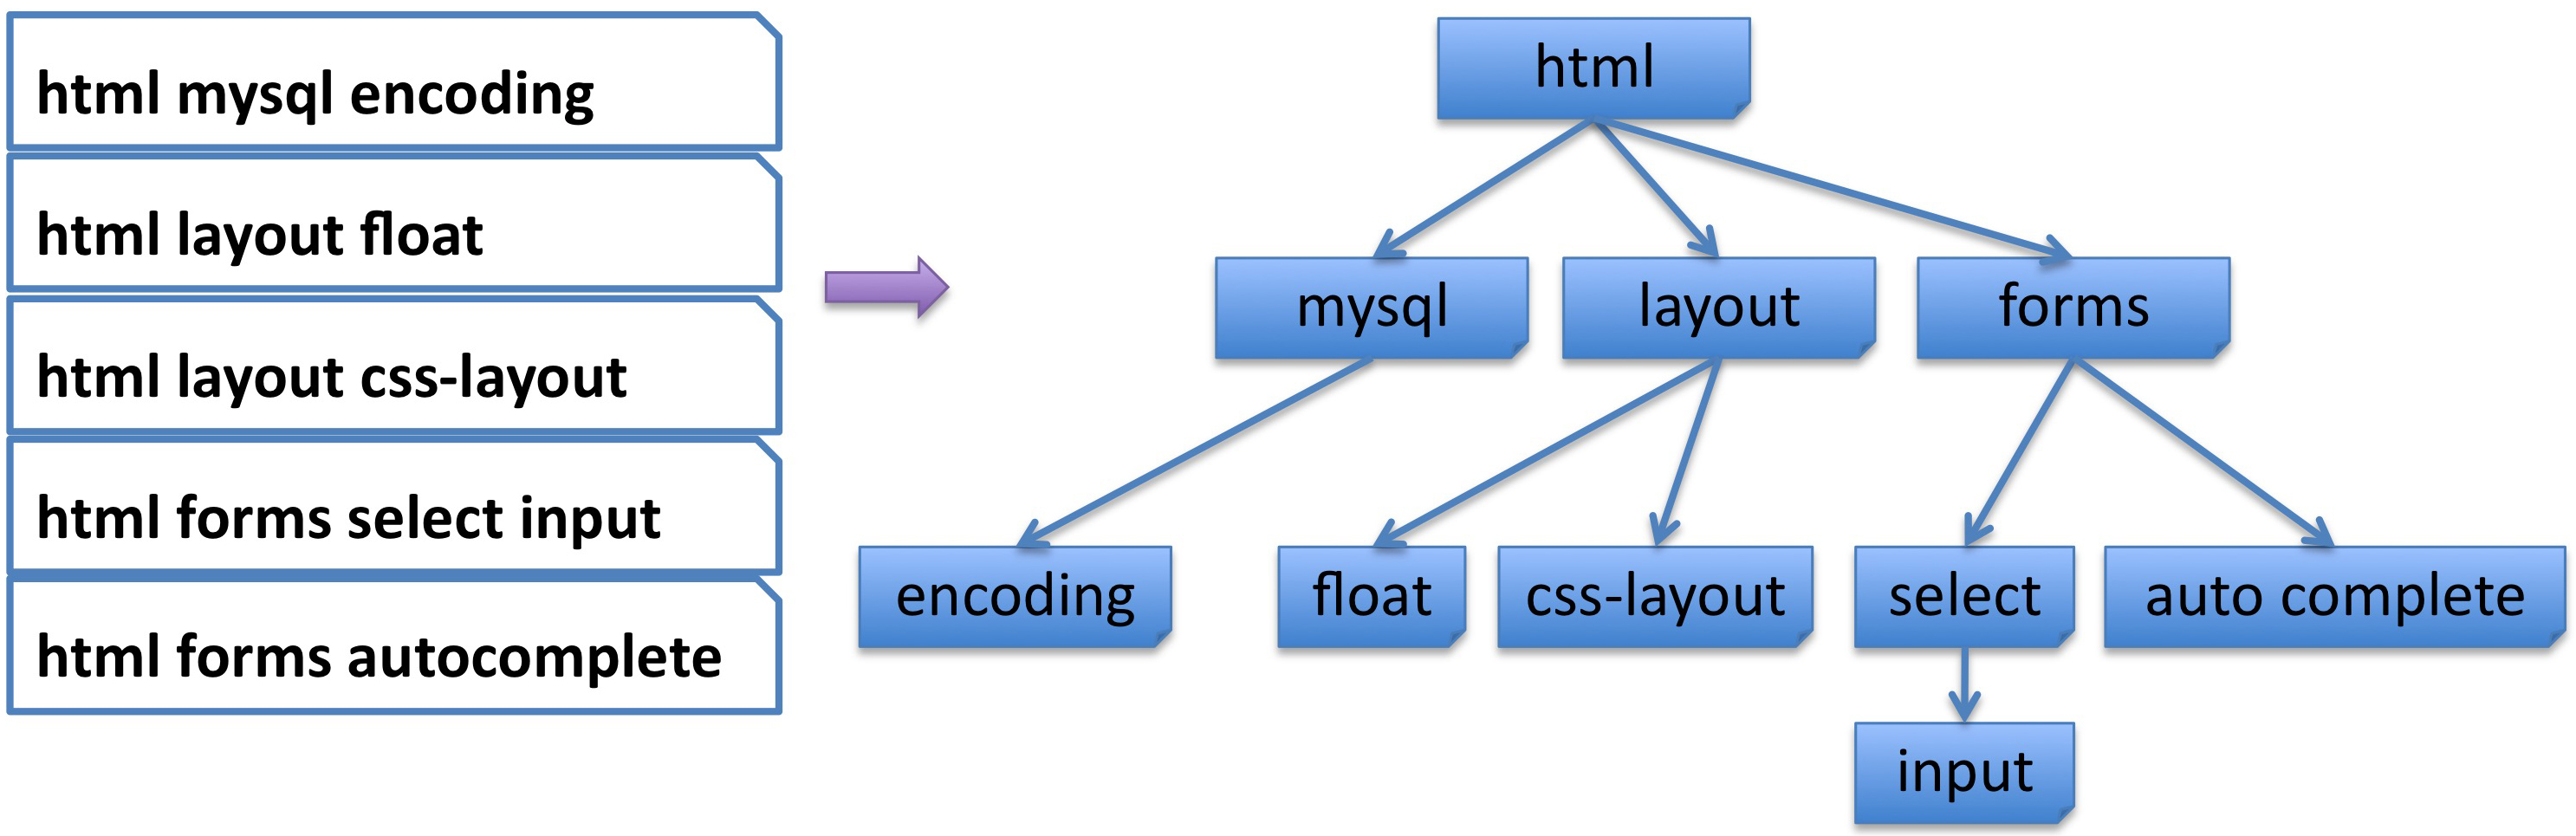
\includegraphics[width=5in]{buildTreeProcess.jpg}  
\caption{Example of a tag tree}
\label{fig:tagtree} 
\end{figure}


%\IncMargin{2em}

\begin{algorithm}%[htp]
\begin{algorithmic}[1]
\label{algo:algotopic}
\State \textbf{Input:} \textit{ enriched tag list of questions, topic number K}
\State \textbf{Output:} \textit{topic-tag distribution}
\State \textit{/*build trees process, shown in Fig \ref{fig:tagtree}*/}

\State trees = null \textit{/* initialize */}
\For { \textit{tag} \textbf{in} \textit{taglist} }%{tag question's taglist}
\State{trees.insert(taglist)}
\EndFor
\State \textit{/*build affinity matrix for root\_tags*/}
\State root\_tags = trees.get\_root\_tags() 
\State   affinities\_matrix = \textbf{build\_affinity}(root\_tags) 
\State  \textit{/*run spectral-clustering on affinity matrix*/}
\State  groups = \textbf{spectral}(\textit{affinities\_matrix,K})
\State  \textit{/*combine tree according to groups*/}
\State  new\_trees = \textbf{combine\_tree} (\textit{trees,groups})   
\State  \textit{/*compute topic-tag distribution*/}
\State  topic\_distributions = \textbf{compute} (\textit{new\_trees})
\State \textit{** we perform a spectral clustering to divide these root tags into several groups}
\end{algorithmic}
\end{algorithm}
%\caption{Topic Extraction}

In the \textit{build trees} process (lines 3-6), we build a tag tree according to the position of tags in a question, and record the occurrence of each node. For example, let us consider again the tag lists of questions Q1, Q2, Q3 in Figure~\ref{fig:examplefirsttag}. Based on them, we construct two trees. The root of the first tree is \textit{html}, the occurrence of this node is \textit{2}, it has only one child \textit{css}, which has \textit{2} occurrences, and this node has two children, \textit{layout} and \textit{height}, and each one occurs \textit{1} time. The root of the second tree is \textit{c\#} with \textit{1} occurrence.

By processing all the tag lists, many trees are generated. We then construct an affinity matrix of the root nodes (lines 7-9). Since we applied our first-tag enrichment method, the number of root tags is not very large. The similarity of two root nodes is computed according to equation \ref{eq:simi}:


\begin{equation}
Simi(R_i,R_j)= \frac{I(R_i,R_j)}{(I(R_i)+I(R_j))}
\label{eq:simi}
\end{equation}

where $I(R_i,R_j)$ denotes the co-occurrence of root tag $R_i$ and root tag $R_j$, and $I(R_i)$ and $I(R_j)$ denote the occurrence of root tag $R_i$ and root tag $R_j$ respectively. Then we perform a spectral clustering~\cite{Ng01onspectral} on the affinity matrix to group these root nodes  (line 10-11). Each group forms what we will call a topic. As spectral clustering requires to select the desired number of topics, we choose the same number \textit{30} as~\cite{Chang:2013}, which has proved to be a reasonable setting for the Stackoverflow dataset.

We then combine trees if their root nodes belong to the same topic (lines 12-13). This process leads to a forest where each tree represents a topic. Then, in the \textit{compute topic-tag distribution} process (lines 14-15), for each topic tree, we compute $p(t|k)$, which denotes the probability of tag $t$ belong to topic $k$, by using the Maximum Likelihood estimation (MLE), according to equation \ref{eq:laplace}: 
%TODO: MLE as not been explained, referenced of even expended in the text above.
%DONE

\begin{equation}
%\begin{split}
p(t|k) = \frac{p(t,k)}{p(k)} = \frac{I(t)+1}{\sum I(t)+N}
\label{eq:laplace}
%\end{split}
\end{equation}

%\begin{equation}
%p(tag|topic)= \frac{p(tag,topic)}{p(topic)} = \frac{I(tag)}{I(sum(tag))}
%\label{eq:computesub}
%\end{equation}

where $I(t)$ denotes the number of occurrences of tag $t$ in the topic tree $k$, and $\sum I(t)$ denotes the total number of occurrences of all tag occurrences in the topic tree.

\begin{figure}[!htp]
\centering
%\epsfig{file=fly.eps, height=1in, width=1in} % use this if you use "pdflatex"
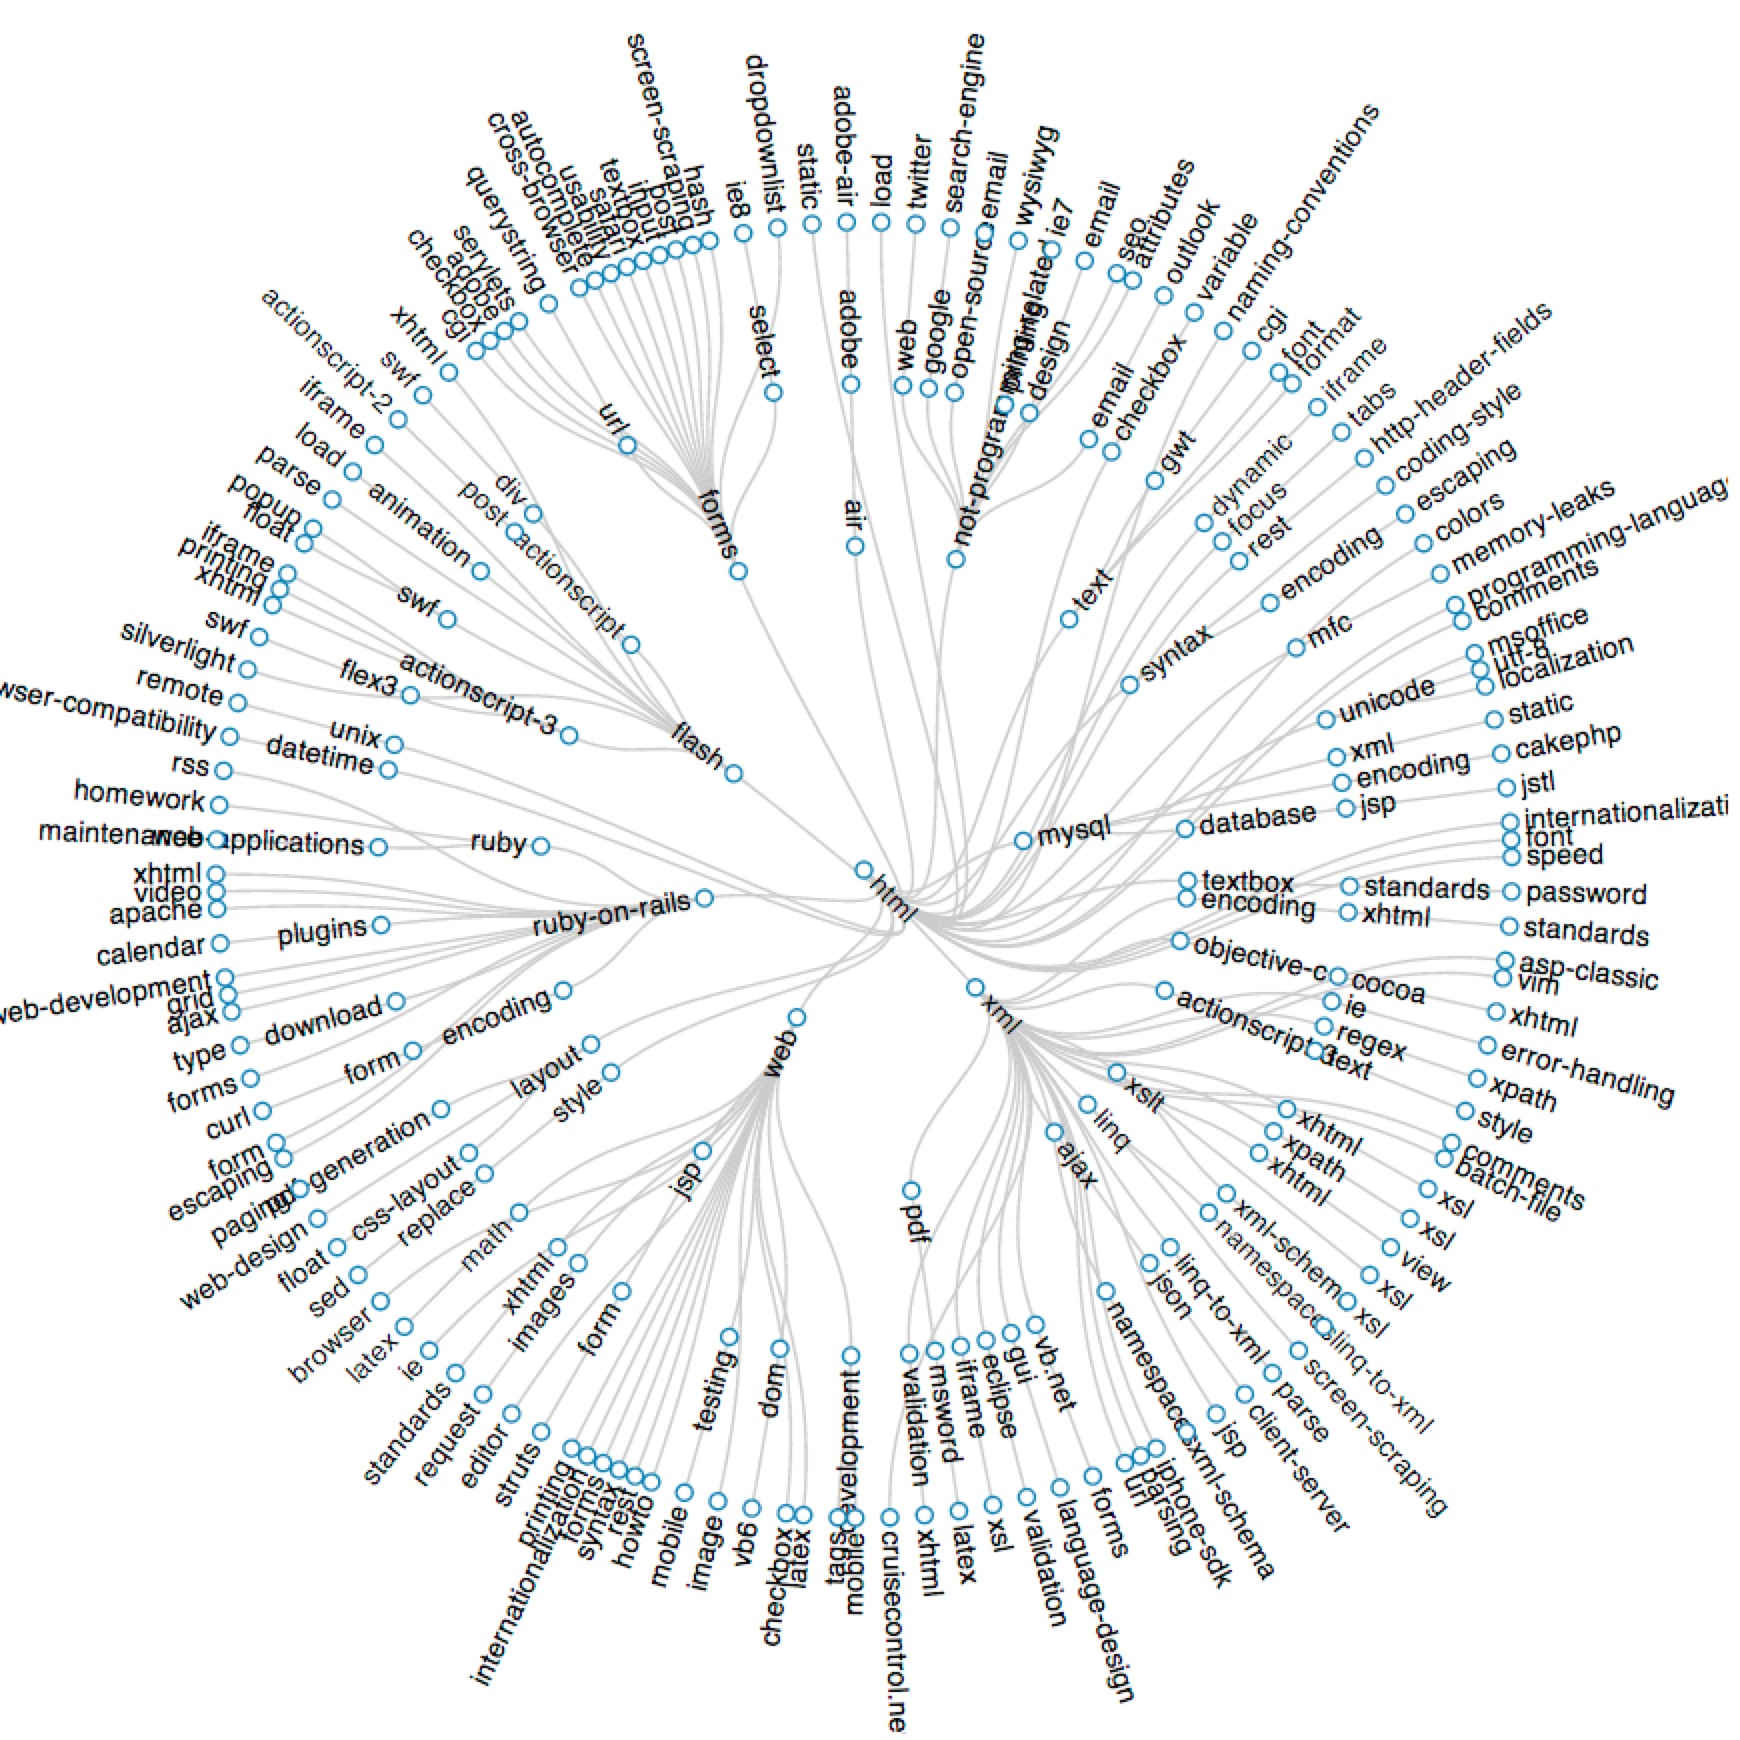
\includegraphics[width=5in]{tag_prefixtree.png}  
\caption{\textit{html}'s tag tree}
\label{fig:htmltagtree} 
\end{figure}

%$p$ and $I(p)$ respectively denote the probability and the number of occurrences of a parent tag, $p\_sub\_i$ and $I(sub\_i)$ denote the probability and the number of occurrences of the $i-th$ child tag. We estimate the probability of $p\_sub\_i$ by equation \ref{eq:computesub},
%\begin{small}
%\end{small}
%p\_sub\_i=\frac{I(sub_i)}{I(p)} * p

Compared with LDA-based model, our model could have a zero-probabilities problem, with less popular or new tags related to some topics with a zero probability due to no evidence of co-occurrence. For example, if tag \textit{zombie-process} never occurs in a \textit{html}-related tag tree, then the probability of tag \textit{zombie-process} to be related to \textit{html-related} topics is zero, which could lead to some problems when dealing with young datasets. We avoid it by using the Laplace smoothing method, as shown in equation \ref{eq:laplace}. Table \ref{tab:toptagspttd} shows the top tags and their probabilities detected by our method.

% TODO: integrate proof here, in this paper that says LDA needs hundreds of iterations to find stable results.\cite{griffiths2004finding}
%DONE
In addition, compared with LDA-based model, our model is much simpler and faster. The probabilistic graphical model requires hundreds of iterations to get stable results~\cite{griffiths2004finding}.

We used the spectral clustering implementation of scikit-learn toolkit\footnote{Scikit-learn toolkit: \\ \indent \url{http://scikit-learn.org/stable/modules/clustering.html#spectral-clustering}}. We only run it on the set of root nodes, which has quite a small size (around 1175 nodes after the tag enrichment process), which means that we only need to build an affinity matrix on these root nodes and the overall cost therefor remains acceptable.

\subsection{User Interest Detection: assigning users to topics}
\label{sec:uidetect}
In StackOverflow, users answering a question can be considered as interested in the topics denoted by the tags of the question. As a result, a starting point for user interest detection is to model the initial situation as follows: a user answering a question acquires the tags attached to this question and gradually, each user acquires a list of tags.

So we represent a user by a tag list: $U= \{U_i | i=1,...,n\},U_i=\{tag_i|i=m,n,...,k\}$, and our goal is, for each user $U_i$, to find $I_i=\{I_{i1},I_{i2}...I_{ik}\}$ where $I_{ik}$ denotes the probability of user $U_i$ to be related to $topic_k$. As we already have a topic-tag distribution %(see section \ref{subsec:topicextraction})
we simply compute the user-topic distribution according to equation \ref{eq:getuserinterest} where $P_{t,k}$ denotes the probability of tag $t$ to be related to topic $k$. We then normalize the probabilities between 0 and 1 by dividing the global max value. We use the $log$ function for numerical stability. Here we do not apply normalization at the level of the user, because like \cite{yang2013community}, we believe that each user could have a high interest in two or more topics simultaneously, while most of the probabilistic graphical models including LDA and PLSA require that the sum of all the probabilities is 1, which means that a user cannot have high probabilities to many topics simultaneously. Our method does not have this limitation. 

Then we identify users' communities of interests based on the user-topic distribution: a user having a high probability for a topic should be a member of the community represented by this topic.

\begin{equation}
 I_{i,k} = log \left\{\sum_{t=1}^{v} P_{t,k}  +1 \right\}\\
  %\begin{cases}
  %* :\text{if } tag_t \in U_i
  %\end{cases}
\label{eq:getuserinterest}
\end{equation}
%0       & \text{if } tag_t \notin U_i \\




\section{TTD Experiments and Evaluation on StackOverflow data}\label{sec:TTDexperiment} 
We conducted experiments on the dataset of activities on StackOverflow between 2008 and 2009, which is available online\footnote{\url{https://archive.org/details/stackexchange}}, to evaluate the performance of our TTD approach compared to three other community detection algorithms. 
%\subsection{Dataset Description}
Some basic statistics of the dataset are given in Table \ref{tab:stackoverflowdataset}. We see that the total number of users arround 100K and among them, 47K users submitted at least one question, and 54K users answered at least one question. The total number of tags attached to questions is 24K, and 20\% of them are used more than 10 times. The frequency of tags follows a power law distribution. The total number of posts is 1.1M; among them there are 242K questions and 870K answers. If two users answer the same question, then the two users are wired by a co-answer link. We filtered the co-answer links with a rule stating that a link is kept if two users answer the same questions more than 10 and 20 times. As a result, we obtained two noise-less datasets. 

% TODO: I uncommented the table and referenced it from the text please check it.
%DONE

\begin{table}[htp]
\caption{Basic statistics of the stackoverflow dataset}
\label{tab:stackoverflowdataset}
\centering
\begin{tabular}{|c|c|c|c|c|}
\hline
\textbf{item} & \textbf{description} \\
\hline
total users & 103K (47K questioner, 54K answerer)\\
\hline
total tags & 24K (20\% used more than 10 times)\\
\hline
total posts & 1.1M (question 242K, answer 870K) \\
\hline
co\_answer\_10 & 902 users, 6746 co\_answer link\\
\hline
co\_answer\_15 & 401 users, 2326 co\_answer link\\
\hline
co\_answer\_20 & 241 users, 1064 co\_answer link\\
\hline
co\_answer\_25 & 153 users, 592 co\_answer link\\
\hline
labeled user & 902 users, 1$\sim$3 labels per user\\
\hline
\end{tabular}
\end{table}

% TODO: I uncommented the figures but they need to be checked and commented in the text. 
%DONE

% TODO: include all the figures, charts, graphics, etc. you have, add a label and caption and comment them in the text
%DONE

%new version of this image is in discusstion section.
%
%\begin{figure}[htp]\centering
%\epsfig{file=fly.eps, height=1in, width=1in}
%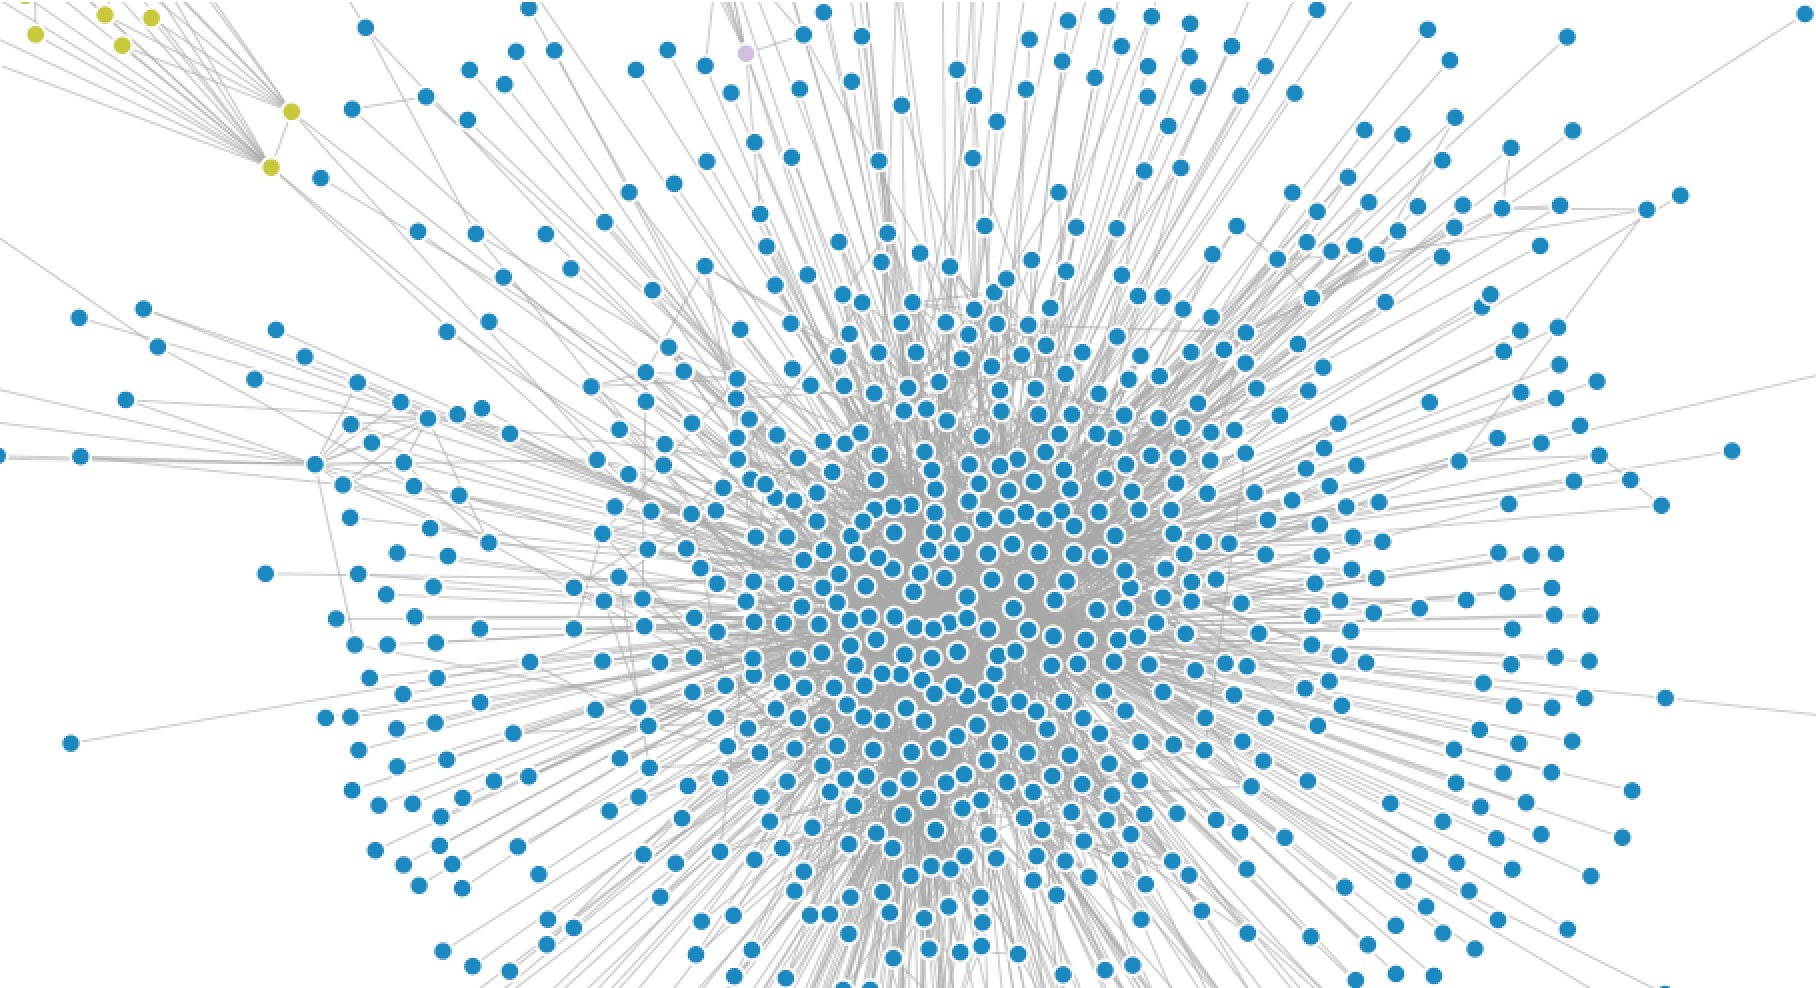
\includegraphics[width=5in]{lpa_co_answer_10.png}  % use this if you use "pdflatex"
%\caption{\# of user answered and asked question}
%\label{fig:qaheatmap} % Fig.2
%\end{figure}

% TODO: why is the following text here ? duplicate with last section ?
%DONE
% i comment this part because dont use user study section.
%Then we manually labeled the 'co\_answer\_10' 902 users to evaluate the results obtained on the four datasets by comparing them with our manual labelling.
%\subsection{Evaluations}
%\vspace{-2em}

\subsection{Performance of Topic Extraction: perplexity metric}
We use the Perplexity~\cite{blei2003latent} metric to measure the topic extraction performance. It is a common metric in the topic modeling area, measuring how well the words in test documents are represented by the word distribution of extracted topics. The intuition is that a better model will tend to assign higher probabilities to the test dataset, corresponding to a lower perplexity value. We split the dataset (question tag lists), 80\% as training set, 20\% as testing set.
% TODO: do we need to to a k-fold cross validation or not?
% TBD
We run LDA and our method on the training set to get the topic distribution. Then for a test set of M questions' tag lists ($N_d$ denotes the number of tags in the $d^{th}$ question) the Perplexity score is computed as shown in equation \ref{eq:gettagperplexity}:
%\begin{small}
\begin{equation}
  Perplexity(D_{test})=exp\left\{-\frac{\sum_{d=1}^{M}\log p(t)}{\sum_{d=1}^{M}N_d}\right\}
\label{eq:gettagperplexity}
\end{equation}

\begin{figure}[htp]
\centering
%\epsfig{file=fly.eps, height=1in, width=1in}
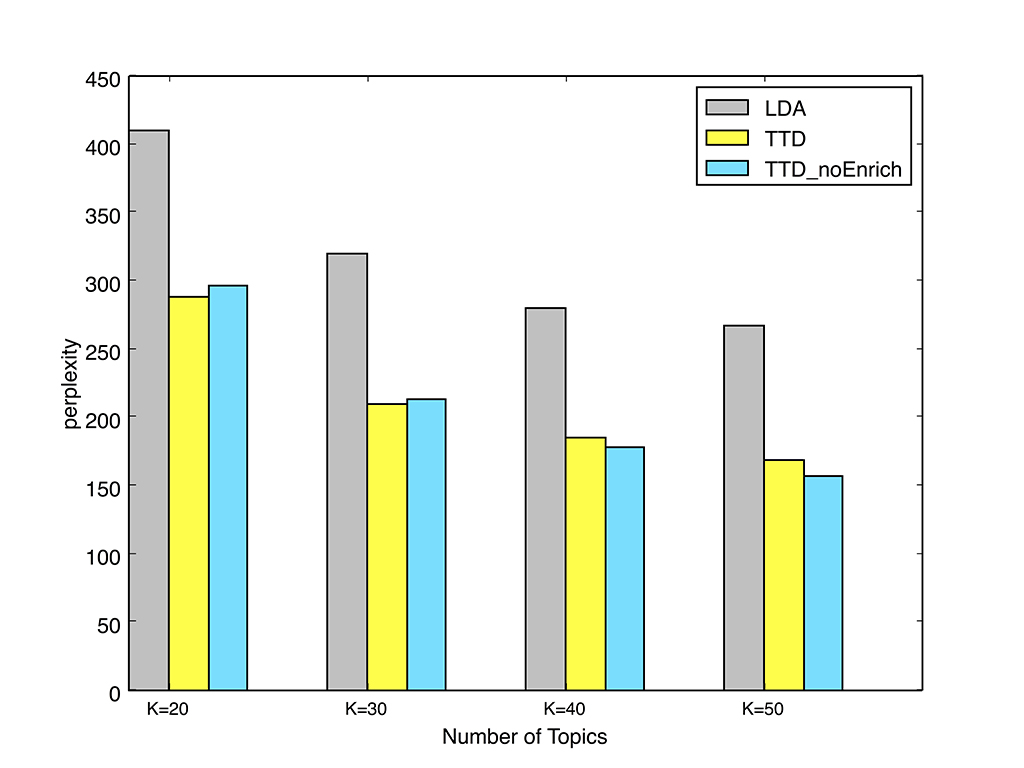
\includegraphics[width=5in]{perplexity.jpg}  % use this if you use "pdflatex"
\caption{Comparison of topic extraction performances}
\label{fig:tagperplexity} 
\end{figure}

In our model, $p(t)$ is equal to $p(k|q)*p(t|k)$. We compute the topic-question distribution $p(k|q)$ similarly to the user-topic distribution (see Section \ref{sec:uidetect}), by replacing user's tag lists by question's tag lists. The only difference is that we normalize the question-topic distribution to make sure that the sum of a question's topic distribution is 1. We show and compare the average perplexity score in Figure \ref{fig:tagperplexity}. \textit{TTD} is our method, \textit{TTD\_noEnrich} represents our method without first-tag enrichment. We find that TTD could outperform the state-of-the-art LDA method. The reason is that, compared with traditional document topic modeling use cases, question tag lists in Q\&A sites are very short, and LDA performs poorly in this situation. Besides, our first-tag enrichment method can improve the performance when the number of topics is not very large. 

We use different discount functions, which is used in equation \ref{eq:accumulate}, and compare the perplexity score. we found that the performance of using discount is better than not using discount. And the liner discount is better than exponential discount. 
% 1 0.8 0.6 0.4 0.2:    212  liner
% 1 0.5 0.25 0.125 :    213  exponential
% 1 1 1 1 1        :    215  not using

Another point is that, benefiting from a tree structure for topics, we can easily extract sub-topics from a given topic. Besides, TTD is based on a topic model, so extracting these sub-topics can help us find sub-communities within a detected community. Table \ref{tab:comparedwithsubtopic} shows the top tags of \textit{java}'s sub-topic \textit{html} and of topic \textit{html}. We can find that the differences are noticeable for topics: a user who is interested in topic \textit{html} is not necessarily interested in \textit{java}'s sub-topic \textit{html} and vice versa. 

\begin{table}[htp]
%\begin{table}[!t]
\caption{Top tags and their probabilities for some topics computed with TTD}
\label{tab:toptagspttd}
\centering
%\scriptsize
%\begin{tabular}{|p{37pt}|p{10pt}|p{31pt}|p{10pt}|p{43pt}|p{10pt}|}
\begin{tabular}{|c|c|c|c|c|c|}

\hline
\multicolumn{2}{|c|}{topic4} & \multicolumn{2}{c|}{topic5} & \multicolumn{2}{c|}{topic6}  \\
\hline
iphone&0.203&git&0.198&sql&0.177\\
\hline
objective-c&0.112&svn&0.096&mysql&0.122\\
\hline
ios&0.109&version-control&0.045&sql-server&0.074\\
\hline
xcode&0.042&github&0.033&database&0.040\\
\hline
cocoa-touch&0.021&tfs&0.033&oracle&0.030\\
\hline
ipad&0.020&maven&0.029&sql-server-2008&0.029\\
\hline
cocoa&0.018&tortoisesvn&0.018&tsql&0.026\\
\hline
uitableview&0.012&msbuild&0.016&query&0.025\\
\hline
ios5&0.010&jenkins&0.015&sql-server-2005&0.019\\
\hline
core-data&0.009&tfs2010&0.014&database-design&0.011\\
\hline
\hline
\multicolumn{2}{|c|}{topic12} & \multicolumn{2}{c|}{topic13} & \multicolumn{2}{c|}{topic14}   \\
\hline
html&0.214&javascript&0.264&machine-learning&0.247\\
\hline
css&0.201&jquery&0.114&artificial-intelligence&0.130\\
\hline
xhtml&0.017&html&0.035&neural-network&0.062\\
\hline
web-development&0.016&ajax&0.031&classification&0.046\\
\hline
ie&0.012&css&0.016&data-mining&0.037\\
\hline
css-layout&0.010&firefox&0.013&svm&0.031\\
\hline
div&0.010&dom&0.011&weka&0.025\\
\hline
layout&0.010&php&0.011&libsvm&0.015\\
\hline
firefox&0.009&ie&0.010&nlp&0.024\\
\hline
ie6&0.009&web-development&0.008&bayesian&0.011\\
\hline
\end{tabular}
\end{table}

\begin{table}[htp]
\caption{Top tags for \textit{java}'s sub-topic \textit{html} and \textit{mysql}, denoted by java\_html, and java\_mysql respectively, compared with topics \textit{html} and \textit{mysql}}
\label{tab:comparedwithsubtopic}
\centering
%\tiny
\begin{tabular}{|p{0.8in}|p{4.2in}|}
%\begin{tabular}{|c|l|}
\hline
java\_html& jsp swing xml parsing jsf jeditorpane pdf applet dom\\
\hline
html & css xhtml web-development table div ie layout css-layout firefox\\
\hline
\hline
java\_mysql&jdbc hibernate database tomcat prepared-statement spring connection-pooling connection security \\
\hline
mysql &database query mysql-query ruby-on-rails database-design performance stored-procedures innodb optimization\\
\hline
\end{tabular}
\end{table}

\subsection{Performance of User Interest Detection: Similarity metrics}
Traditional community detection algorithms are based on a network structure. As there is no explicit network in our dataset and in order to compare our work with other approaches on the same dataset, we extracted a network of interactions between users: a co-answer network inspired by the notion of co-view network introduced in~\cite{DBLP:conf/icwsm/GargiLMY11}. The idea behind it is that if two users answer the same question they share some of their interests. So, the co-answer network, to some extent, can reflect the common interests between users. We filtered the co-answer links with a rule stating that a link is kept if two users answer the same questions more than 10 times and 20 times.
% TODO: in a PhD thesis there is no size constraint so you should give all your experiments 10 to 25
%DONE, add 20.

Based on the noise-less dataset obtained, we implemented three well known community detection methods in order to compare our approach with them.

In order to evaluate the results of overlapping community detection, for each user, a method should output $1\sim3$ community labels with corresponding probabilities to indicate to what extent the user is interested in the community. Then we define three levels of interest in a community: \textit{High}, \textit{Medium}, \textit{Low} according to the probabilities. In addition, we empirically set the number of communities to $30$ for all the evaluated methods.
\begin{itemize}
\item{SLPA~\cite{DBLP:journals/csur/XieKS13}}: An overlapping community detection method inspired by a classical Label propagation algorithm (LPA). SLPA algorithm can evaluate to which extent a user belongs to a community by the received propagated label (a 'Post-process' in SLPA algorithm). So, it can output more than one community label according to these frequencies.
\item{LDA}: Similar to~\cite{yang2013cqarank}, we run LDA to build a user-topic-tag model on the given dataset, users are represented by their tag list. As the output contains a user-topic distribution, we just sort the distribution for each user and choose the top 3 topic labels as community label together with their probabilities.
\item{Clustering}: We used the implementation of hierarchical clustering from scikit-learn toolkit\footnote{\url{http://scikit-learn.org/stable/modules/clustering.html#hierarchical-clustering}}. As clustering algorithms are hard-partitioned, it can only generate one group label for each user.
\item{TTD}: it is our method. We sort the results of user interest detection (section \ref{sec:uidetect}) and choose the top 3 as community label together with their probabilities.
\end{itemize}

% TODO: you noted that "this part still need to improve..... to do work."
% forgot it...

Our aim was to evaluate the similarity between users within a detected community of interest. We mainly used the \textit{jaccard similarity} and \textit{cosine similarity} of two user's tag lists to evaluate the similarity of two user's interests. We used a modified modularity metric to compute the difference between the average similarity between the users within a community ($avg\_inner$) and the average similarity between the users in a community and some user randomly chosen from the whole dataset ($avg\_rand$). This is captured in Equation \ref{eq:nmi}, where $N$ represents the number of users in a community $C$, and $Simi$ denotes the similarity function. $Rand\_U$ represents users that are randomly chosen from the whole data set. A higher value of $avg\_inner$ denotes that users within a community are very similar. A lower value of $avg\_rand$ denotes that users of a community are not very similar to random users. So a higher value of $modularity$ means a larger difference between $avg\_inner$ and $avg\_rand$, which is considered as a better partition of communities. As the metric has random variables, we run the experiments 10 times and each time we used different random users. Besides, we created a \textit{center} user in each community by averaging all users' tag lists and frequencies, then we computed the average similarity between each user in a community and this \textit{center} user as $avg\_center$. 
As introduced before, each method gives $1\sim3$ community labels for each user to indicate the level of interest. So we evaluated each level of interest respectively.

\begin{equation}
%\tiny
%\begin{split}
  M(C) \\
  =\frac{Avg\_inner(\sum_{i=1}^{N}\sum_{j=1}^{N} Simi(U\_i,U\_j))}{Avg\_rand(\sum_{i=1}^{N}\sum_{j=1}^{50} Simi(U\_i,Rand_U\_j))}
\label{eq:nmi}
%\end{split}
\end{equation}

Experiment results are shown in Table \ref{tab:uidcompare10} and \ref{tab:uidcompare20}. We run each method on the co-answer-10 and co-answer-20 dataset 10 times, and listed the average value. We found that our method is better than the three other methods in detecting users' \textit{High} level of interest with both metrics. The reason why our method is not very efficient to detect users' \textit{Low} level of interest is that our method allows users to belong to more than one community with high probabilities, since our method do not have the sum-to-one constrain. For example, a user could be interested in a topic with a probability of 0.7 (High) and interested in several topics with a probability of 0.3 (Low), where the sum of these probabilities not equal to 1. Then this user will be in many \textit{Low} level of interest communities. This puts some irrelevant users with \textit{Low} level of interest which decreases the similarity between community members.




\begin{sidewaystable}

%\begin{table*}[htp]
\caption{Comparison of the performances of the methods of user interest detection on co\_answer\_10 dataset}
\label{tab:uidcompare10}
%\tiny
\scriptsize
\centering
%\begin{tabular}{|p{60pt}||p{60pt}||p{60pt}|}
%\begin{tabular}{|p{23pt}|p{23pt}|p{23pt}|p{23pt}|p{23pt}|p{23pt}|p{23pt}|p{23pt}|p{23pt}|p{23pt}|p{23pt}|p{23pt}|p{23pt}|}
\begin{tabular}{|c|c|c|c|c|c|c|c|c|c|c|c|c|}

\hline
Similarity & \multicolumn{12}{c|}{Jaccard Similarity}  \\
\hline
Level  &  \multicolumn{4}{c|}{High Interest} & \multicolumn{4}{c|}{Medium Interest} &  \multicolumn{4}{c|}{Low Interest} \\
\hline
Metric  & avg\_inner & avg\_rand & \textit{modularity} & avg\_center& avg\_inner & avg\_rand & \textit{modularity} & avg\_center& avg\_inner & avg\_rand & \textit{modularity} & avg\_center \\
\hline
TTD&\textbf{0.162}&\textbf{0.033}&\textbf{4.909}&\textbf{0.218}&\textbf{0.135}&\textbf{0.039}&\textbf{3.462}&0.171&0.107&0.042&2.548&0.131\\
\hline
LDA&0.147&0.035&4.200&0.178&0.131&0.039&3.359&\textbf{0.177}&\textbf{0.144}&0.041&\textbf{3.512}&\textbf{0.193}\\
\hline
SLPA&0.131&0.040&3.275&0.166&0.129&0.040&3.225&0.159&0.121&\textbf{0.039}&3.103&0.155\\
\hline
Clustering&0.130&0.041&3.171&0.161&0.000&0.000&0.000&0.000&0.000&0.000&0.000&0.000\\
\hline
Similarity & \multicolumn{12}{c|}{Cosine Similarity}  \\
\hline
Level  &  \multicolumn{4}{c|}{High Interest} & \multicolumn{4}{c|}{Medium Interest} &  \multicolumn{4}{c|}{Low Interest} \\
\hline
Metric  & avg\_inner & avg\_rand & \textit{modularity} & avg\_center& avg\_inner & avg\_rand & \textit{modularity} & avg\_center& avg\_inner & avg\_rand & \textit{modularity} & avg\_center \\ 
\hline
TTD&0.736&\textbf{0.574}&\textbf{1.282}&0.857&0.573&\textbf{0.602}&0.952&0.761&0.475&0.629&0.755&0.695\\ \hline
LDA&\textbf{0.836}&0.660&1.267&\textbf{0.917}&\textbf{0.900}&0.612&\textbf{1.471}&\textbf{0.948}&\textbf{0.757}&\textbf{0.600}&\textbf{1.262}&\textbf{0.865}\\ \hline
SLPA&0.749&0.624&1.200&0.854&0.590&0.621&0.950&0.687&0.702&0.625&1.123&0.844\\ \hline
Clustering&0.763&0.622&1.226&0.875&0.000&0.000&0.000&0.000&0.000&0.000&0.000&0.000\\ \hline
\end{tabular}
%\end{table*}

\end{sidewaystable}




\begin{sidewaystable}

%\begin{table*}[htp]
\caption{Comparison of the performances of the methods of user interest detection  on co\_answer\_20 dataset}
\label{tab:uidcompare20}
%\tiny
\scriptsize
\centering
%\begin{tabular}{|p{60pt}||p{60pt}||p{60pt}|}
%\begin{tabular}{|p{23pt}|p{23pt}|p{23pt}|p{23pt}|p{23pt}|p{23pt}|p{23pt}|p{23pt}|p{23pt}|p{23pt}|p{23pt}|p{23pt}|p{23pt}|}
\begin{tabular}{|c|c|c|c|c|c|c|c|c|c|c|c|c|}

\hline
Similarity & \multicolumn{12}{c|}{Jaccard Similarity}  \\
\hline
Level  &  \multicolumn{4}{c|}{High Interest} & \multicolumn{4}{c|}{Medium Interest} &  \multicolumn{4}{c|}{Low Interest} \\
\hline
Metric  & avg\_inner & avg\_rand & \textit{modularity} & avg\_center& avg\_inner & avg\_rand & \textit{modularity} & avg\_center& avg\_inner & avg\_rand & \textit{modularity} & avg\_center \\
\hline
TTD&\textbf{0.175}&0.034&5.121&\textbf{0.232}&\textbf{0.153}&0.038&4.025&\textbf{0.189}&0.115&0.043&2.695&0.132\\
\hline
LDA&0.160&\textbf{0.028}&\textbf{5.742}&0.198&0.139&0.030&\textbf{4.623}&0.188&\textbf{0.174}&0.037&\textbf{4.697}&\textbf{0.224}\\
\hline
SLPA&0.126&0.029&4.290&0.167&0.057&\textbf{0.014}&4.104&0.078&0.064&\textbf{0.015}&4.394&0.087\\
\hline
Clustering&0.164&0.038&4.303&0.206&0.000&0.000&0.000&0.000&0.000&0.000&0.000&0.000\\
\hline
Similarity & \multicolumn{12}{c|}{Cosine Similarity}  \\
\hline
Level  &  \multicolumn{4}{c|}{High Interest} & \multicolumn{4}{c|}{Medium Interest} &  \multicolumn{4}{c|}{Low Interest} \\
\hline
Metric  & avg\_inner & avg\_rand & \textit{modularity} & avg\_center& avg\_inner & avg\_rand & \textit{modularity} & avg\_center& avg\_inner & avg\_rand & \textit{modularity} & avg\_center \\ 
\hline
TTD&0.676&\textbf{0.594}&1.138&0.818&0.548&0.621&0.883&0.745&0.471&0.644&0.730&0.690\\ \hline
LDA&\textbf{0.858}&0.627&\textbf{1.367}&\textbf{0.926}&\textbf{0.888}&\textbf{0.608}&\textbf{1.462}&\textbf{0.939}&\textbf{0.755}&\textbf{0.610}&\textbf{1.237}&\textbf{0.865}\\ \hline
SLPA&0.729&0.632&1.152&0.845&0.695&0.630&1.104&0.834&0.679&0.632&1.074&0.826\\ \hline
Clustering&0.762&0.627&1.216&0.875&0.000&0.000&0.000&0.000&0.000&0.000&0.000&0.000\\ \hline
\end{tabular}
%\end{table*}

\end{sidewaystable}






Table \ref{tab:ourmodelresult} shows some users and their interests detected with TTD and their top 10 tags. The first row contains user ids, the second row contains their detected communities of interests with their probabilities. The following ten rows show the top 10 tags for each user. We replaced community labels by names assigned according to the tags associated to each topic of interest.


\begin{sidewaystable}

%\begin{table}[htp]
\caption{Examples of user interests detected with TTD}
\label{tab:ourmodelresult}
%\scriptsize
\centering
%\begin{tabular}{|p{60pt}|p{60pt}|p{60pt}|}
\begin{tabular}{|c||c||c|}
\hline
user\_10224&user\_103043&user\_113570\\
\hline
database (0.805)\newline c\#-dev (0.081)&java-dev (0.664)\newline database (0.105)&c\#-dev (0.393)\newline web-dev (0.328)\\
\hline
sql-server (21)&java (135)&c\# (107)\\
%\hline
sql (21)&swing (28)&jquery (89)\\
%\hline
tsql (6)&oracle (27)&javascript (56)\\
%\hline
performance (4)&sql (23)&.net (47)\\
%\hline
database (4)&subjective (15)&asp.net (27)\\
%\hline
stored-procedures (3)&windows (13)&css (23)\\
%\hline
sql-server-2005 (3)&eclipse (12)&regex (20)\\
%\hline
.net (3)&best-practices (12)&html (20)\\
%\hline
mysql (2)&plsql (10)&iphone (12)\\
%
sql-server-2000 (2)&regex (10)&string (10)\\
\hline
user\_24181&user\_34509&user\_30461\\
\hline
web-dev (0.743), database (0.072)&c-dev (0.663), linux-dev (0.083)&ios-dev (0.885), linux-dev (0.020)\\
\hline
php (304)&c++ (703)&cocoa (333)\\
%\hline
javascript (193)&c (187)&objective-c (184)\\
%\hline
mysql (116)&templates (62)&iphone (47)\\
%\hline
html (86)&stl (53)&cocoa-touch (39)\\
%\hline
css (57)&linux (48)&osx (35)\\
%\hline
regex (40)&subjective (45)&mac (34)\\
%\hline
jquery (37)&pointers (44)&iphone-sdk (20)\\%
%\hline
sql (27)&java (42)&xcode (18)\\
%\hline
ajax (26)&bash (40)&cocoa-bindings (18)\\
%\hline
apache (23)&boost (31)&core-graphics (18)\\
\hline
\end{tabular}
%\end{table}


\end{sidewaystable}




%TODO: why is the following text commented ?
%DONE  I think it may cause bias because of the human judgement since it's complained by many reviewers

\subsection{User Study: ranking users' interested topics}
In order to evaluate the quality of whether a user is correctly assigned to the right interest group, and to which extent the user belongs to the interest group. To achieve this, we conducted a user survery on the dataset by inviting 2 volunteers as annotators. We asked a volunteer to manually label 902 users (refer to the co\_answer\_10 dataset) by assigning each user up to 3 labels out of eight group labels, chosen from \textit{c-development} group, \textit{java-development} group, \textit{c\#-development} group, \textit{web-development} group, \textit{ios-development} group, \textit{database} group, \textit{linux-development} group and \textit{other-topic} group. 
For example, if user A sequentially has three group labels, \textit{java-development},\textit{web-development},\textit{ios-development}, it means that user A has a big interest in the group \textit{java-development}, a medium interest in the group \textit{web-development}, a lower interest in the group \textit{ios-development}. Since each user has an ordered label list, we have to evaluate both the correctness of detected groups and the correctness of the order. 
We ask another volunteer (who was not involved in labeling the 902 users) to label the results of the methods with the same 8 labels.
As SLPA algorithm can detect overlapping communities. She was asked to assign an interest group name, from the 8 labels, to each community according to users tag lists in each community, then each user gets at least one interest group name. Besides, SLPA algorithm can evaluate to which extent a user belongs to a community by the frequency (a 'Post-process' in SLPA algorithm). Combined with the interest group name we assigned for each community, SLPA algorithm now can output an ordered interest group name list for each user.
Clustering algorithms can only generate one cluster id for each user, so she was asked to assign an interest group name, from the 8 labels, for each cluster. 
LDA method can give the probability membership to each topic. A high probability indicates that a user is more interested in that group. The volunteer associated the detected 30 topics to the 8 group labels. Then we ordered interest group name list for each user, sorting them by their probabilities. Our approach is treated just like LDA. Here, she just choose the top 3 group name for each user. 
The Normalized DCG (NDCG) is introduced to compare different ranking list. The value of NDCG is between 0.0 and 1.0. In our scenario, a NDCG@p value of 1.0 means detected interests and their order are totally the same as the labeled data till position \textit{p}, while a NDCG@p value of 0.0 means that the detected interests are completely different from the labeled data. For values between 0.0 to 1.0, it means that the detected interests are partially correct or ordered incorrectly. %It still 
Here, we evaluate NDCG@1, NDCG@2, and NDCG@3. The ideal ranking list of each user is the ground-truth and corresponding score is 10, 8 and 6. Fig \ref{fig:allinone} shows the result of NDCG performance for each method. 
\begin{figure}[hp]
\centering
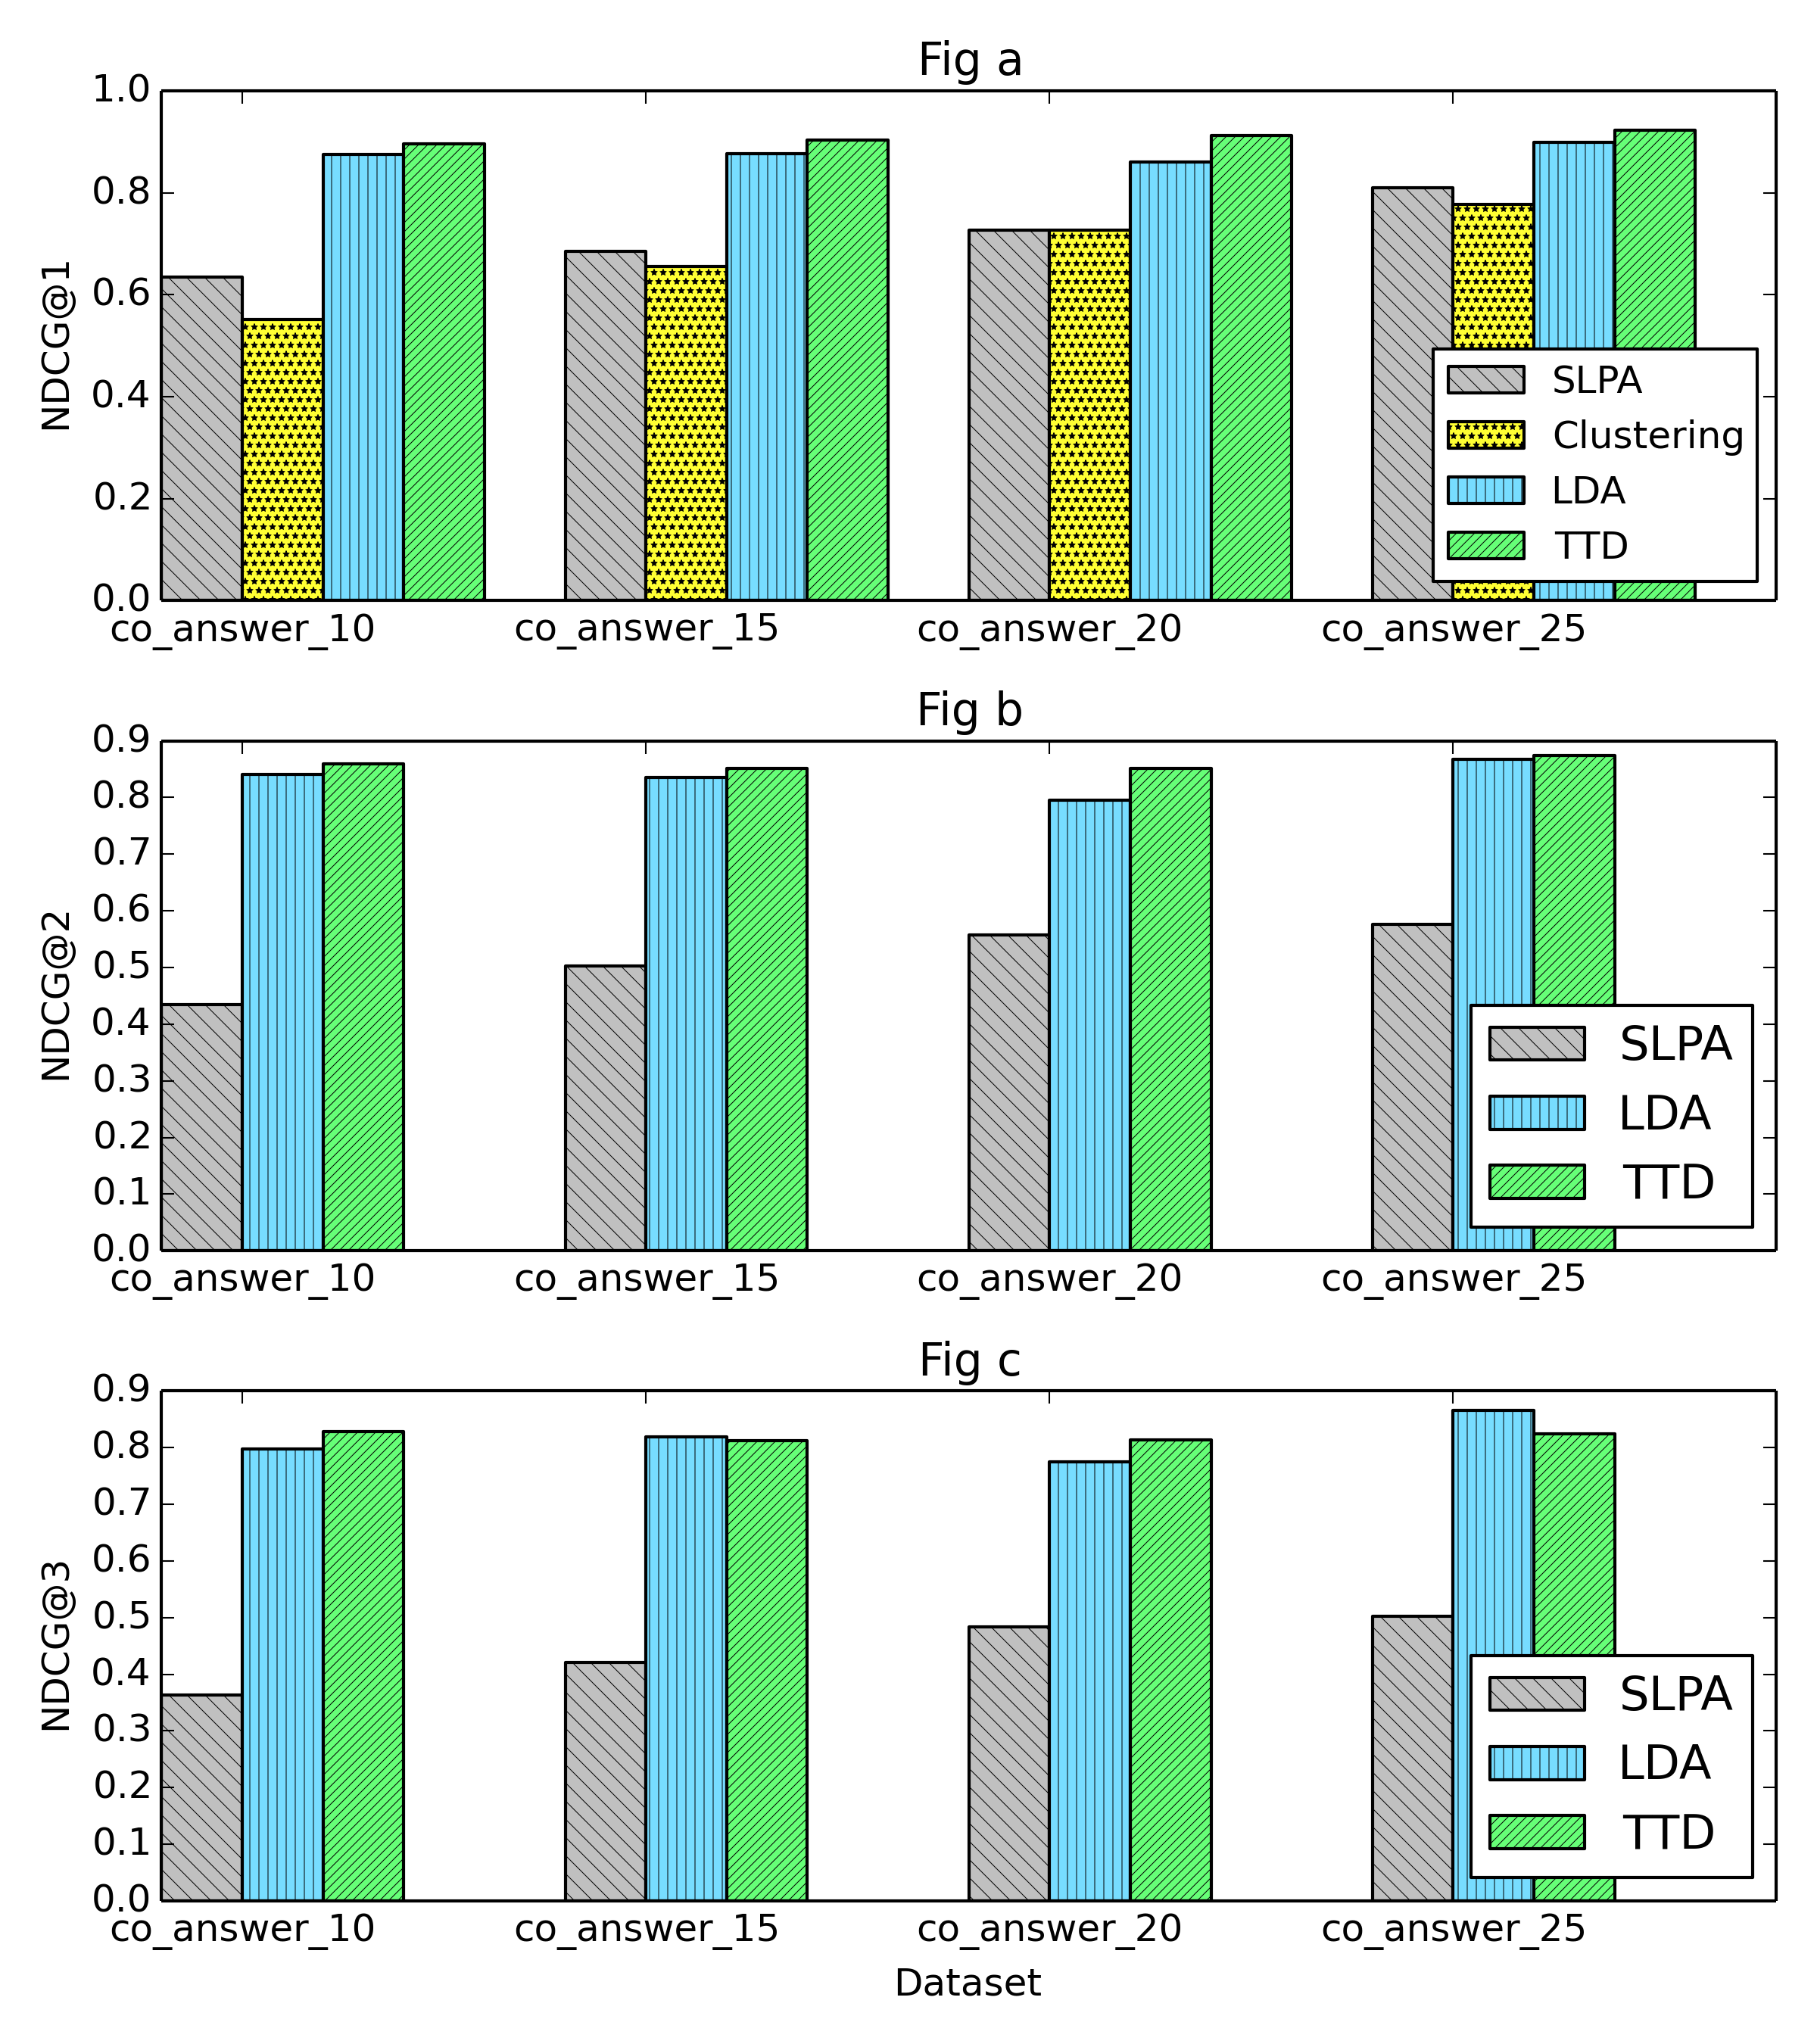
\includegraphics[width=5in]{all_in_one.png} 
\caption{NDCG results comparaison}
\label{fig:allinone} % Fig.2
\end{figure}
NDCG@1 reflects the prominent interest detected by each algorithm compared with the ground-truth of user's prominent interest. We noticed that our Empirical method is partially better than LDA, and outperforms SLPA and hierarchical clustering. We also mention that with the dataset becoming less noisy (people have prominent and clear-intention interests), all methods' performance increase. The same phenomenon is also observed in NDCG@2,3. As hierarchical clustering algorithms give a hard partition there are no performance comparison for hierarchical clustering algorithm in NDCG@2,3. Although there is limitation in the user study because that the ground-truth is the human judgement label, which may have some bias. It still worth to do this experiment because that the similarity experiment focus more on the community, but this user study experiment focus more on each user.


\subsection{Scalability: topic based user assignment is scalable}
We also evaluated the scalability of each method. However, as these methods are written in different programming languages, it is not fair to consider this as a precise evaluation; it is just an indication. To increase the stability of the comparison, we run experiments 10 times, and listed the average values. We used a Java implementation of LDA algorithm. All the other methods were implemented in Python. For our method, the time of topic detection was also counted in. For LDA and SLPA, we set the iteration number at 100. We run the experiments on a computer with 3GHz Intel i7 CPU and 8GB RAM. From the experiment, we could find that LDA, SLPA and our method are linear in terms of the number of users. Although LDA algorithm is theoretically $O(nm)$ in each iteration, with $n$ representing the number of users, and $m$ representing the number of tags for each user, when we test it on large datasets, it clearly appears that only $n$ actually has an impact; $m$ has a very low impact. So LDA could be regarded as linear. Besides, \cite{griffiths2004finding} proved that LDA model requires a few hundreds of iterations to obtain stable topic distribution. Our model does not have this limitation.
\begin{figure}[htp]\centering
%\epsfig{file=fly.eps, height=1in, width=1in}
%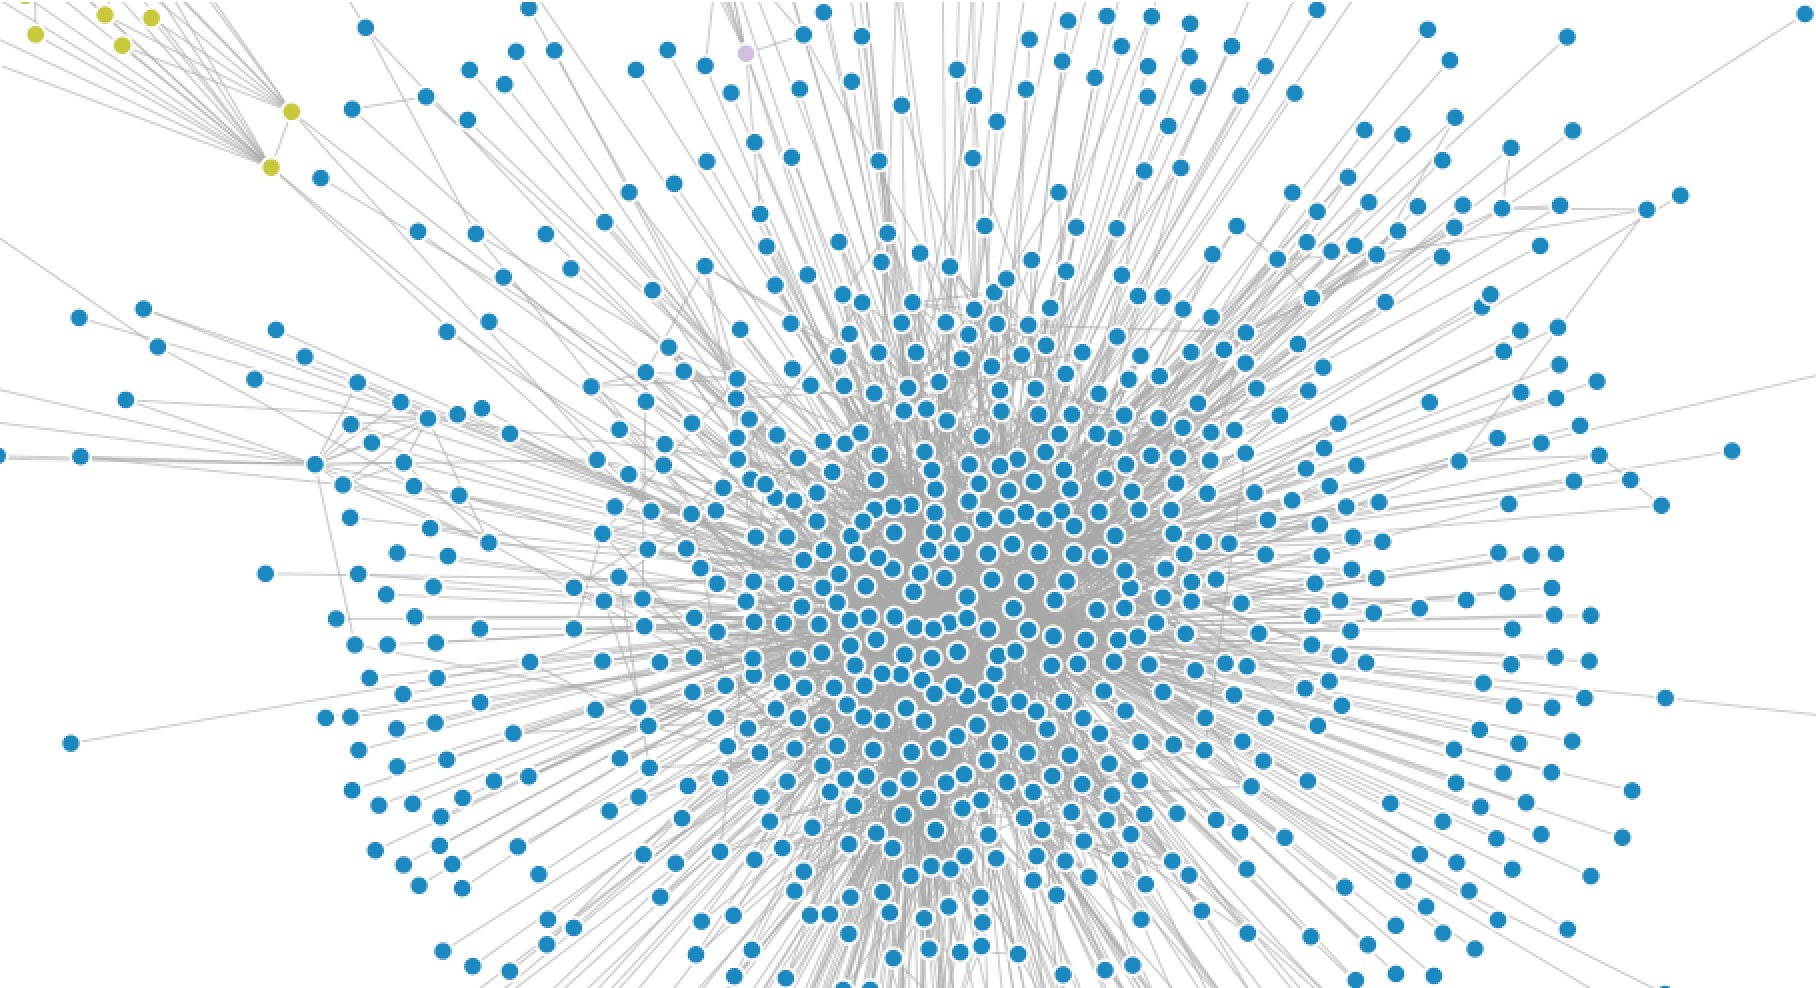
\includegraphics[height=2in, width=3.2in]{lpa_co_answer_10.png}  % use this if you use "pdflatex"
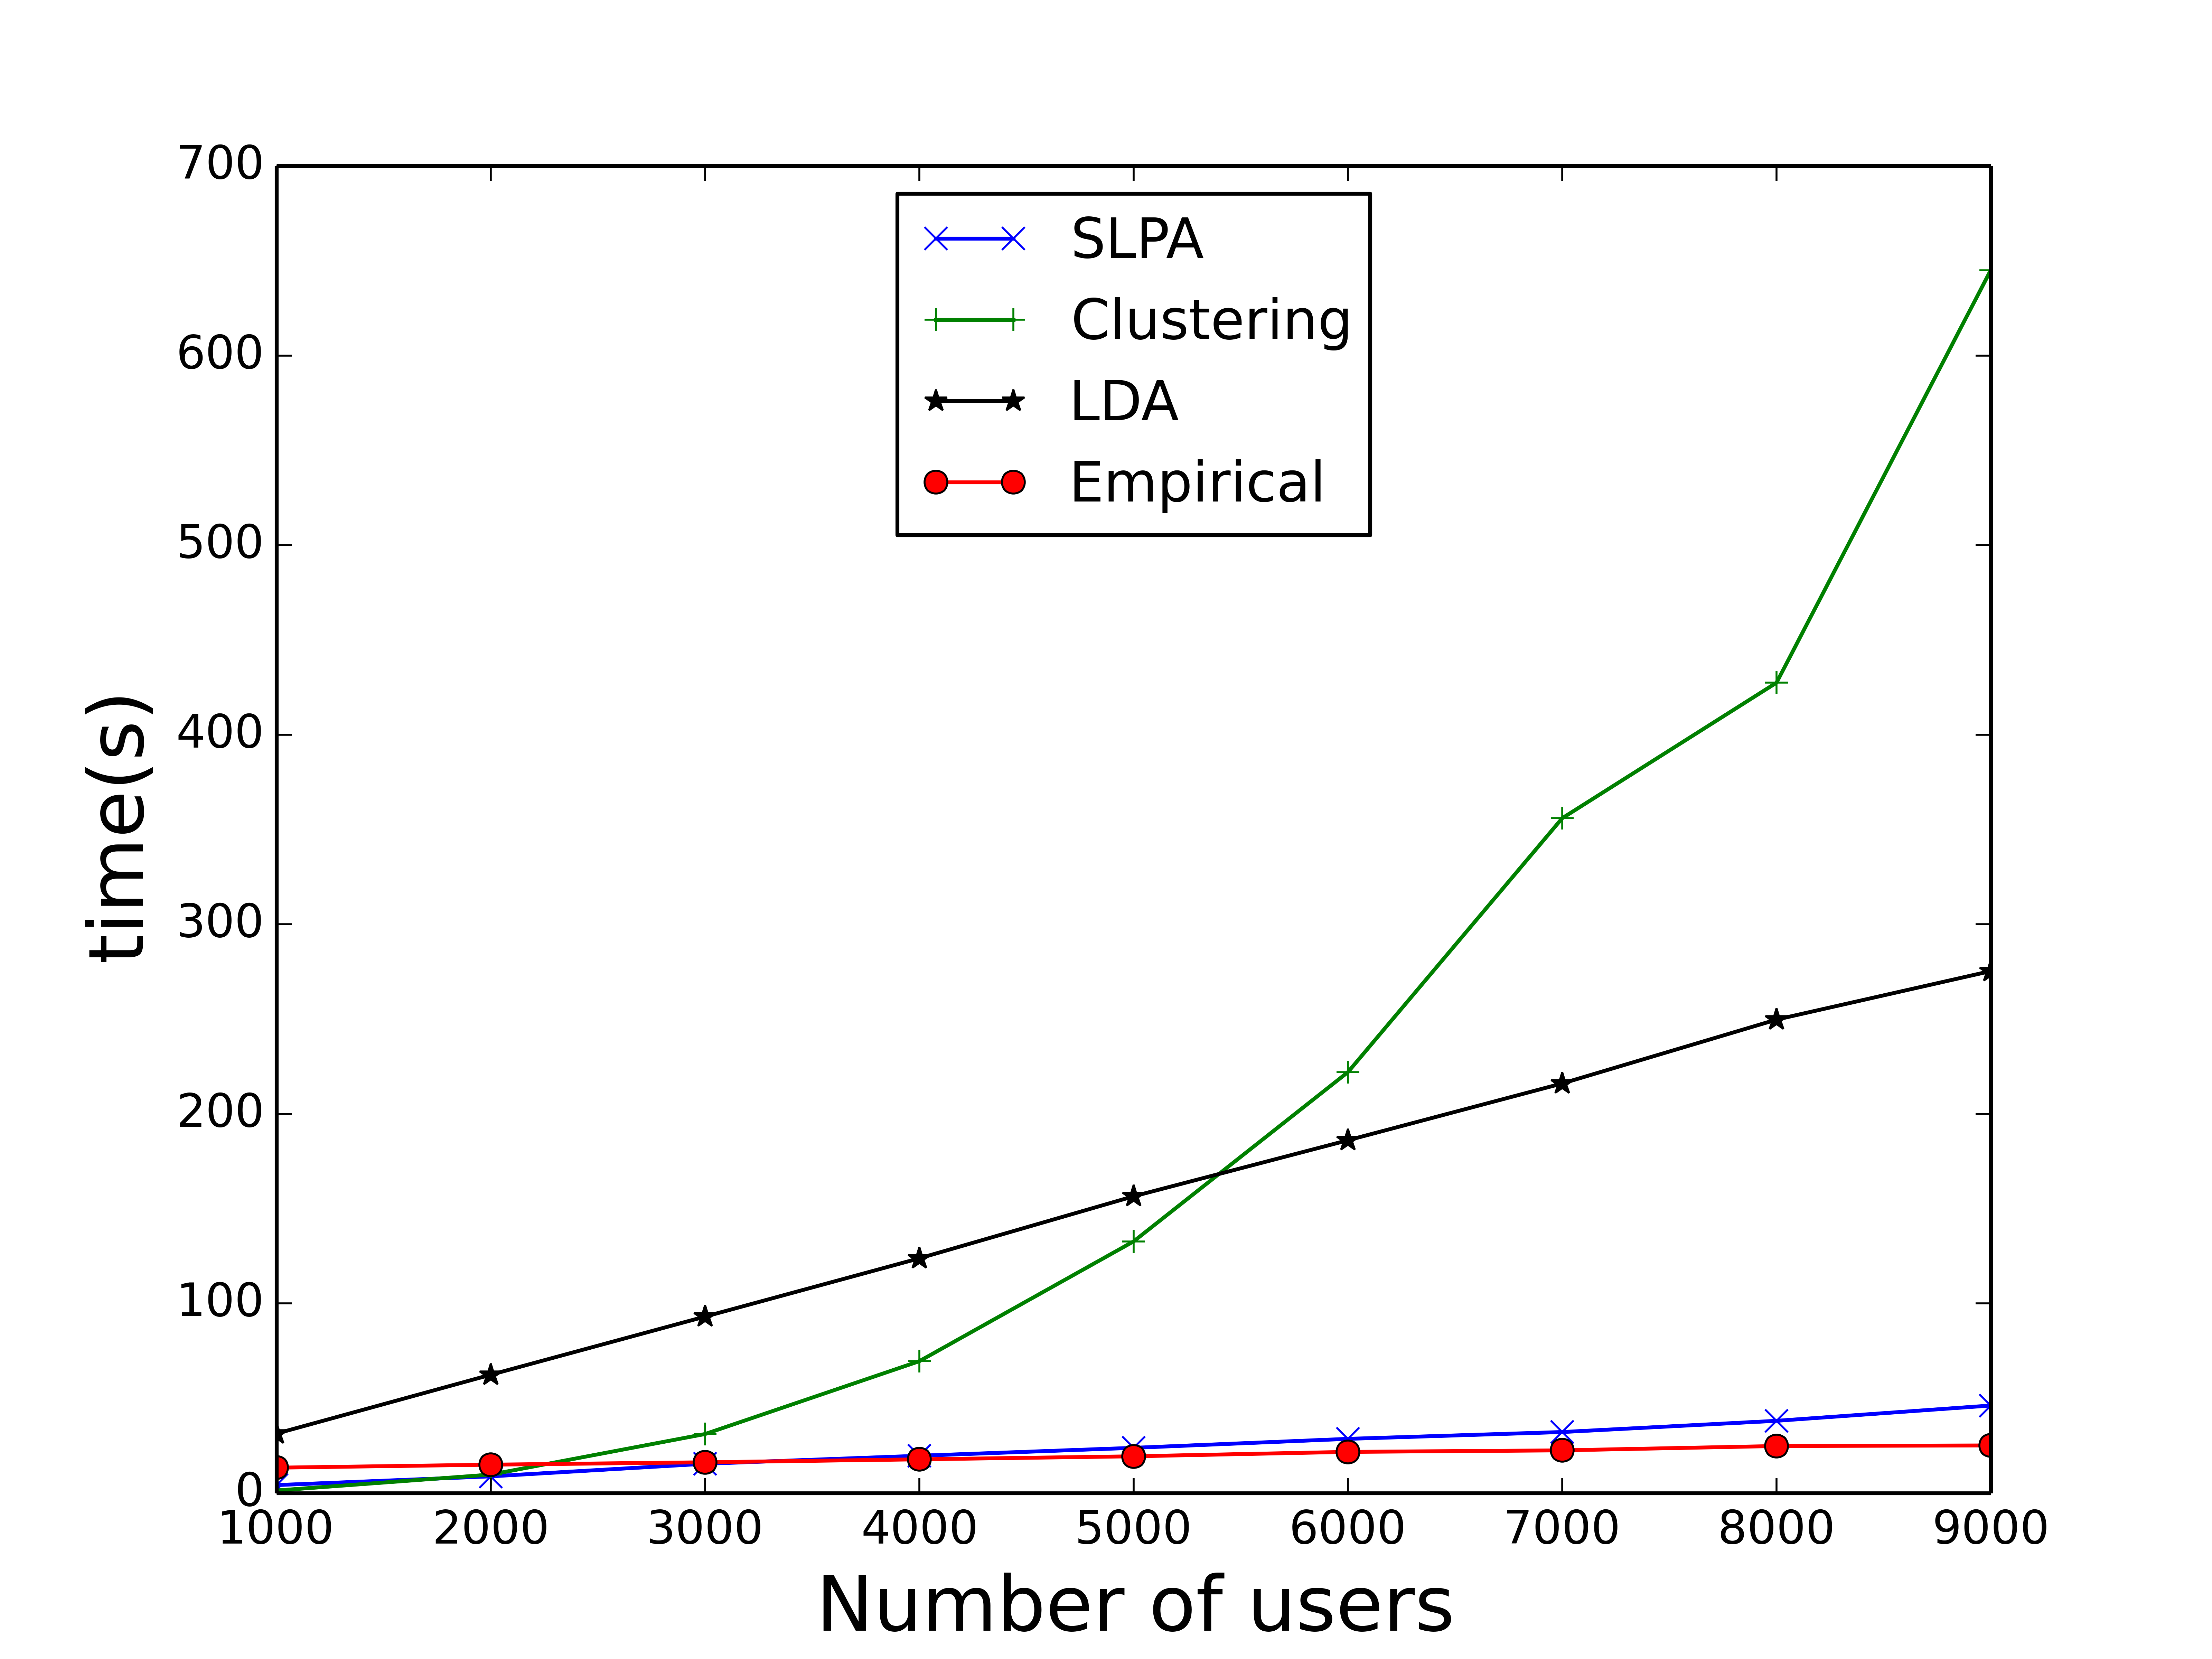
\includegraphics[width=5in]{time_perfor.jpg} 
\caption{Scalability of the compared user interest detection methods}
\label{fig:scalability} % Fig.2
\end{figure}

% TODO: you need to report your evaluation on Flickr to validate on other datasets. 
%DONE

\subsection{Genericity of the proposed Topic Extraction Method}
In order to test that whether our proposed topic extraction methods is generic, we collected a dataset from flickr\footnote{flickr website: \url{https://www.flickr.com/} } which contains 1211499 photos attached with tags. For instance, a photo tagged with \{\emph{china} \emph{pinyao}\} indicates the location information. A photo tagged with \{\emph{night} \emph{people} \emph{bar}\} describes the time and content information. We run our topic extraction method on this dataset, and we list some results in Table \ref{tab:flickrdataset}. We can find that the detected topics are interesting. For example, topic 3 includes photos which contains airplanes, topic 24 includes photos which contains bicycles, and topic 23 includes photos taken in cities of Italy.
\begin{table}[htp]
%\begin{table}[!t]
\caption{Top tags and their probabilities on flickr dataset}
\label{tab:flickrdataset}
\centering
\scriptsize
%\begin{tabular}{|p{43pt}|p{10pt}|p{37pt}|p{10pt}|p{50pt}|p{10pt}|}
\begin{tabular}{|c|c|c|c|c|c|}
\hline
\multicolumn{2}{|c|}{topic3} & \multicolumn{2}{c|}{topic4} & \multicolumn{2}{c|}{topic5}  \\
\hline
airplane&0.074&tshirt&0.216&music&0.077\\ \hline
airport&0.053&shirt&0.154&rock&0.040\\ \hline
aircraft&0.029&shirts&0.112&concert&0.036\\ \hline
flying&0.028&threadless&0.109&live&0.025\\ \hline
plane&0.027&tshirts&0.009&band&0.022\\ \hline
aviation&0.022&tee&0.008&singing&0.019\\ \hline
flight&0.014&clothing&0.007&guitar&0.018\\ \hline
aeroplane&0.012&media&0.006&festival&0.017\\ \hline
jet&0.010&models&0.006&show&0.014\\ \hline
boeing&0.009&camiseta&0.004&livemusic&0.010\\ \hline
\hline
\multicolumn{2}{|c|}{topic23} & \multicolumn{2}{c|}{topic24} & \multicolumn{2}{c|}{topic25}  \\
\hline
italy&0.179&bike&0.114&portrait&0.049\\ \hline
italia&0.053&motorcycle&0.052&girl&0.029\\ \hline
rome&0.028&racing&0.033&woman&0.014\\ \hline
florence&0.021&bicycle&0.028&smile&0.014\\ \hline
venice&0.014&race&0.027&model&0.010\\ \hline
tuscany&0.014&motorbike&0.024&sexy&0.009\\ \hline
roma&0.011&sport&0.019&face&0.008\\ \hline
europe&0.011&speedway&0.011&fun&0.008\\ \hline
firenze&0.010&500cc&0.010&man&0.008\\ \hline
milan&0.007&methanol&0.010&love&0.008\\ \hline
\end{tabular}
\end{table}




\subsection{Discussion: q\&a social network is different}
%This paragraph is used for analysis parameters. TBD
To sum up, most community detection algorithms work well on real-life social networks which contain many \textit{triangle-shape} structures. The interactions between the users in these networks are mainly based on their relationships. It is also noticeable that the relationships which a user in such network can maintain are limited and most likely restricted by the location (co-author networks in academia is also in this situation), so the overall structure of the network is \textit{flatter}, \textit{scattered} and with many \textit{triangle-shape} structures. Comparatively, in Q\&A sites, such as StackOverflow, there are no fixed relationships between users. Users interact with each other based on their own interests. And they are not aware of whom they are interacting with, so they will not maintain explicit relationships. Besides, a user can interact with any other user and mainly interacts with the \textit{"gurus"} (most of questions are answered by a small group of people). So the overall structure of the network is \textit{octopus-shape}~\cite{leskovec2008statistical} with less \textit{triangle-shape} structures. According to~\cite{park2013efficient}, the average number of \textit{triangle-shape} structures per user in Twitter dataset is around $35714$, while in our co-answer-10 dataset, the number of \textit{triangle-shape} structure per user is around $30$ which is far less. So, graph-based community detection methods fail in such situation. The result of SLPA algorithm shows that it outputs one or two giant groups, together with many tiny groups that only contain a small number of users as depicted in Figure \ref{fig:co-answer-network-10}, where each color represents a detected community. We can also see that the network contains less \textit{triangle-shape} structures and a high-density \textit{core}. It also indicates that the network has huge overlaps. However, in co-answer-25 dataset, the graph structure is more \textit{flatter} and contains many \textit{triangle-shape}. Therefore, as shown in figure \ref{fig:co-answer-network-25}, the result of SLPA algorithm outputs several medium sized groups.

% TODO: you need a longer label and a legend for this figure.
%DONE
\begin{figure}[htp]
\centering
%\epsfig{file=fly.eps, height=1in, width=1in}
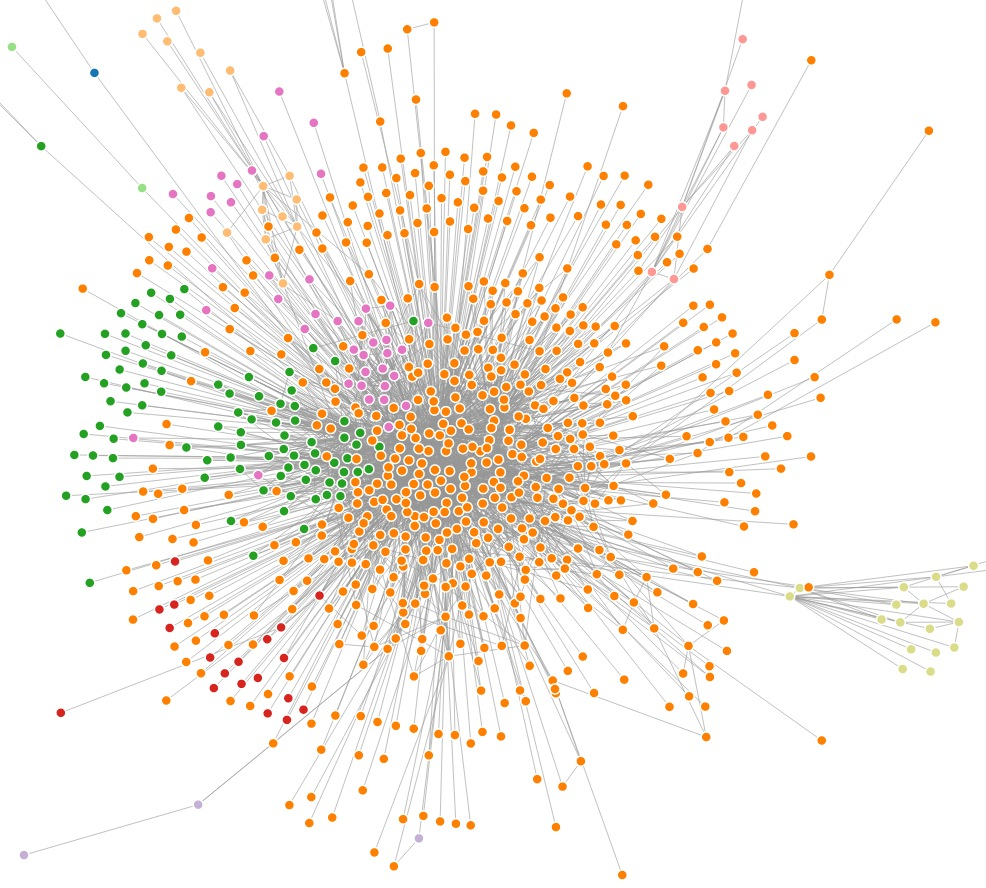
\includegraphics[width=5in]{lpa_10_V2.png}  % use this if you use "pdflatex"
\caption{Illustration of co-answer-network-10, different color indicate detected communities}
\label{fig:co-answer-network-10} % Fig.2
\end{figure}

\begin{figure}[htp]
\centering
%\epsfig{file=fly.eps, height=1in, width=1in}
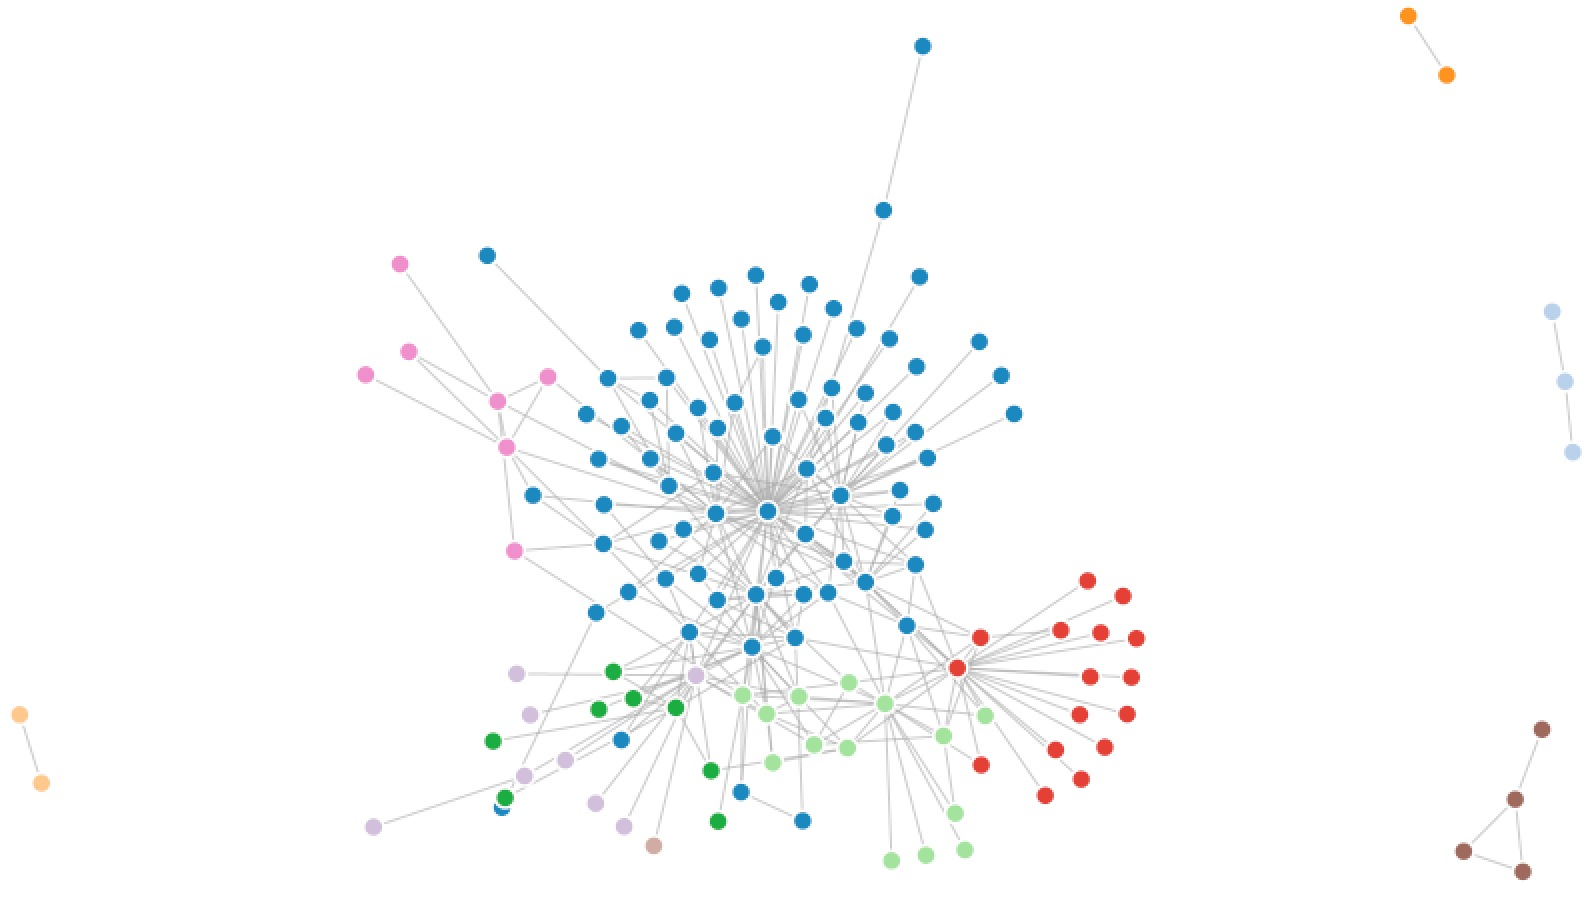
\includegraphics[width=5in]{lpa_co_answer_25.png}  % use this if you use "pdflatex"
\caption{Illustration of co-answer-network-25, different color indicate detected communities}
\label{fig:co-answer-network-25} % Fig.2
\end{figure}
Since clustering methods normally generate hard-partition communities, they cannot detect the overlapping communities which are typical in our case. Concerning the LDA-based methods, on one hand, in our dataset, question tag lists are quite short, and the experiment shows that our topic extraction method gives better results in this situation. On the other hand, the probabilistic graphical model requires hundreds of iterations to get stable results~\cite{griffiths2004finding} which is more complicated and slower than our method. 
\section{Summary: a efficient user topic extraction method}
Recalling our research questions (How can we detect communities of interests in Q\&A sites? How can we also identify the topics that attract them?) we believe that we propose a topic detection method which is very suitable for Q\&A datasets and an efficient user interest detection method to discover topic based overlapping communities of interests. As we found in the topic extraction result, the output are just bag of words with labels such as "topic 15", "topic 30", it is not easy to understand the meaning of the topic by these labels, so we try to tackle this problem in next chapter. The goal will be automatic generate a label for a bag of words.



\chapter{Automatic generation of labels for topics' bags of words}
\doublespacing
\label{chap:label}
\minitoc



\section{Introduction: find labels to represent a topic}
% TODO FAB: I changed this introduction
In naturally language processing and information retrieval, topic modeling classically uses bags of words to represent the meaning a text. However, this is not sufficient to support user interactions as bag of words require an effort from the user to go through the lists of the most important words in order to get an idea of the topic they represent when considered together.
In chapter \ref{chap:ttd} we discussed a method that extracts topics from tags and the outputs of topic model are indeed bags of words, each of them representing a detected topic of interest. At this stage we could only attached meaningless labels for each topic, such as \textit{topic 3}, \textit{topic 5}.

Let us now consider examples of such topics: 
\begin{itemize}
    \item {italy, florence, venice, tuscany -> \textit{Italy}}
    \item {git, svn, tfs, maven -> \textit{version-control}}
    \item {machine-learning, artificial-intelligence, neural-network, classification -> \textit{artificial-intelligence}}
\end{itemize}
The labels, (e.g. \textit{Italy}, \textit{version-control}, \textit{artificial-intelligence}), in the right hand side are good candidates to summarize the overall topic captured by the bags the words on the left hand side. Those labels are at least more informative than labels such as \textit{topic 3} and\textit{topic 5} and can be used in interfaces and graphical representations of the results of the detection of communities of interest.

So an interesting task we consider in this chapter is how to automatically generate a general label for the bags of words representing a topic, which can best represent the meaning of that topic. \cite{chp6OnConceptualLabelingOfBagOfWords} introduce the task of conceptual labelling (CL), which aims at generating a minimum set of conceptual labels that best summarize a bag of words. Our work is similar to this one, but the main difference is that we use DBpedia as external knowledge and we use graph centrality based algorithms to help generate labels to represent a bag of words. \cite{chp2hulpus2013unsupervisedtopiclabeling} also propose to use DBpedia and graph centrality based algorithms to choose label. The difference with our appraoch is that rather than using existing graph centrality based algorithms, we proposed a hybrid method to generate labels. 


\subsection{Problem definition: words, topics and labels}
Our previous work on topic modeling can generate topics from words or tags. Each topic consists of several tags or words. Table \ref{tab:flickrtags} and table \ref{tab:stacktags} list some detected topics from a Flickr dataset and StackOverflow dataset. The topic extraction algorithms are able to put closely related words or tags into the same topic, however, they can only use meaningless IDs (e.g. topic 3) to represent a topic. Our goal in this chapter is to find a label (e.g. aviation) to replace the original label (e.g. topic 3).



\begin{table}[htp]
%\begin{table}[!t]
\caption{Top tags and their probabilities on flickr dataset}
\label{tab:flickrtags}
\centering
%\scriptsize
%\begin{tabular}{|p{43pt}|p{10pt}|p{37pt}|p{10pt}|p{50pt}|p{10pt}|}
\begin{tabular}{|c|c|c|c|c|c|}
\hline
\multicolumn{2}{|c|}{topic3} & \multicolumn{2}{c|}{topic4} & \multicolumn{2}{c|}{topic5}  \\
\hline
airplane&0.074&tshirt&0.216&music&0.077\\ \hline
airport&0.053&shirt&0.154&rock&0.040\\ \hline
aircraft&0.029&shirts&0.112&concert&0.036\\ \hline
flying&0.028&threadless&0.109&live&0.025\\ \hline
plane&0.027&tshirts&0.009&band&0.022\\ \hline
aviation&0.022&tee&0.008&singing&0.019\\ \hline
flight&0.014&clothing&0.007&guitar&0.018\\ \hline
aeroplane&0.012&media&0.006&festival&0.017\\ \hline
jet&0.010&models&0.006&show&0.014\\ \hline
boeing&0.009&camiseta&0.004&livemusic&0.010\\ \hline
\hline
\multicolumn{2}{|c|}{topic23} & \multicolumn{2}{c|}{topic24} & \multicolumn{2}{c|}{topic25}  \\
\hline
italy&0.179&bike&0.114&portrait&0.049\\ \hline
italia&0.053&motorcycle&0.052&girl&0.029\\ \hline
rome&0.028&racing&0.033&woman&0.014\\ \hline
florence&0.021&bicycle&0.028&smile&0.014\\ \hline
venice&0.014&race&0.027&model&0.010\\ \hline
tuscany&0.014&motorbike&0.024&sexy&0.009\\ \hline
roma&0.011&sport&0.019&face&0.008\\ \hline
europe&0.011&speedway&0.011&fun&0.008\\ \hline
firenze&0.010&500cc&0.010&man&0.008\\ \hline
milan&0.007&methanol&0.010&love&0.008\\ \hline
\end{tabular}
\end{table}



\begin{table}[htp]
%\begin{table}[!t]
\caption{Top tags and their probabilities on stackoverflow dataset}
\label{tab:stacktags}
\centering
%\scriptsize
%\begin{tabular}{|p{43pt}|p{10pt}|p{37pt}|p{10pt}|p{50pt}|p{10pt}|}
\begin{tabular}{|c|c|c|c|c|c|}
\hline
\multicolumn{2}{|c|}{topic4} & \multicolumn{2}{c|}{topic5} & \multicolumn{2}{c|}{topic6}  \\
\hline
iphone&0.203&git&0.198&sql&0.177\\
\hline
objective-c&0.112&svn&0.096&mysql&0.122\\
\hline
ios&0.109&version-control&0.045&sql-server&0.074\\
\hline
xcode&0.042&github&0.033&database&0.040\\
\hline
cocoa-touch&0.021&tfs&0.033&oracle&0.030\\
\hline
ipad&0.020&maven&0.029&sql-server-2008&0.029\\
\hline
cocoa&0.018&tortoisesvn&0.018&tsql&0.026\\
\hline
uitableview&0.012&msbuild&0.016&query&0.025\\
\hline
ios5&0.010&jenkins&0.015&sql-server-2005&0.019\\
\hline
core-data&0.009&tfs2010&0.014&database-design&0.011\\
\hline
\hline
\multicolumn{2}{|c|}{topic12} & \multicolumn{2}{c|}{topic13} & \multicolumn{2}{c|}{topic14}   \\
\hline
html&0.214&javascript&0.264&machine-learning&0.247\\
\hline
css&0.201&jquery&0.114&artificial-intelligence&0.130\\
\hline
xhtml&0.017&html&0.035&neural-network&0.062\\
\hline
web-development&0.016&ajax&0.031&classification&0.046\\
\hline
ie&0.012&css&0.016&data-mining&0.037\\
\hline
css-layout&0.010&firefox&0.013&svm&0.031\\
\hline
div&0.010&dom&0.011&weka&0.025\\
\hline
layout&0.010&php&0.011&libsvm&0.015\\
\hline
firefox&0.009&ie&0.010&nlp&0.024\\
\hline
ie6&0.009&web-development&0.008&bayesian&0.011\\
\hline
\end{tabular}
\end{table}

\section{Solution: using DBpedia information}
\label{sec:chp6secSolution}

\subsection{link to DBpedia}

DBpedia\footnote{\url{http://dbpedia.org/about} (accessed Feb 2016)} is a crowd-soured community effort to extract structured information from Wikipedia\footnote{\url{https://www.wikipedia.org/}(accessed Feb 2016)} and makes this information available on the Web. It allows users to link their own dataset to Wikipedia data and to augment it with this huge amount of additional data, documents and links. The DBpedia knowledge base now plays an important role in enhancing the intelligence of Web applications and in supporting information integration. Among the advantages of the DBpedia knowledge base are the fact it covers many domains and that it automatically evolves with Wikipedia changes. It currently describes 38.3 million things in total and contains 3 billion of RDF triples (2014 version).


In order to use the DBpedia knowledge base, a basic step is to link the bag of words to DBpedia. For example, a word \textit{javascript} could be linked to DBpedia resource \textit{\url{http://dbpedia.org/resource/JavaScript}}, a word \textit{beer} could be linked to DBpedia resource	\textit{\url{http://dbpedia.org/resource/Beer}}. However, in some cases, several resources or entities may correspond to the same word (homonymy). For instance, \textit{java} could be linked to the \textit{Java} island but it could also be linked to the\textit{Java}  java programming language. Therefore, we have to deal with a disambiguation problem when linking words to DBpedia resources. This is a well-known problem now and extensively studied by researchers working on entity recognition, named entity detection and entity linking.  Babelfy\cite{chp6babelfy:Moroetal:14tacl} is a unified graph-based approach to solve Entity Linking (EL) and Word Sense Disambiguation (WSD) problems. Their experiments show the state-of-the-art performances on both tasks on 6 different datasets. Moreover they provide an online webservice\footnote{\url{http://babelfy.org} (accessed Feb 2016)}. So we directly use their web API to retrieval DBpedia links for the words in our dataset. In addition, we also use classical similarity metrics to slove disambiguation problem, we detailed them in next subsection.

\subsection{using descriptions' cosine similarity to disambiguation}
Our main dataset is from the StackOverflow website and we found that there are detailed descriptions for each tag on the website, as shown in figure \ref{fig:chp6taginfo}
\begin{figure}[htp]
\centering
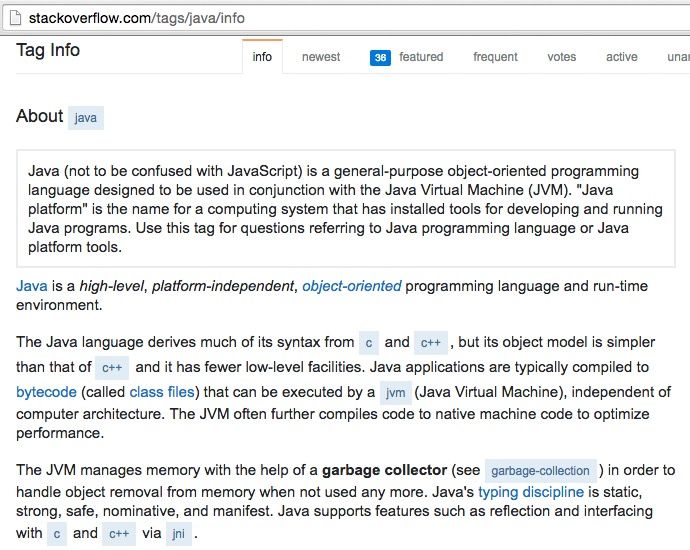
\includegraphics[width=5in]{chp6taginfo.jpg}  
\caption{The description for \textit{java} on StackOverflow dataset \footnote{\url{http://stackoverflow.com/tags/java/info} (accessed Feb 2016)}}
\label{fig:chp6taginfo} 
\end{figure}

Besides, each resource in DBpedia has a description.  We use DBpedia keyword lookup service \footnote{\url{http://dbpedia.org/projects/dbpedia-lookup}(accessed Feb 2016)} to retrieve related resource for each tag. As Shown in Figure \ref{fig:chp6lookup}, results of the lookup service are a lists of resources related to the given keyword.

\begin{figure}[htp]
\centering
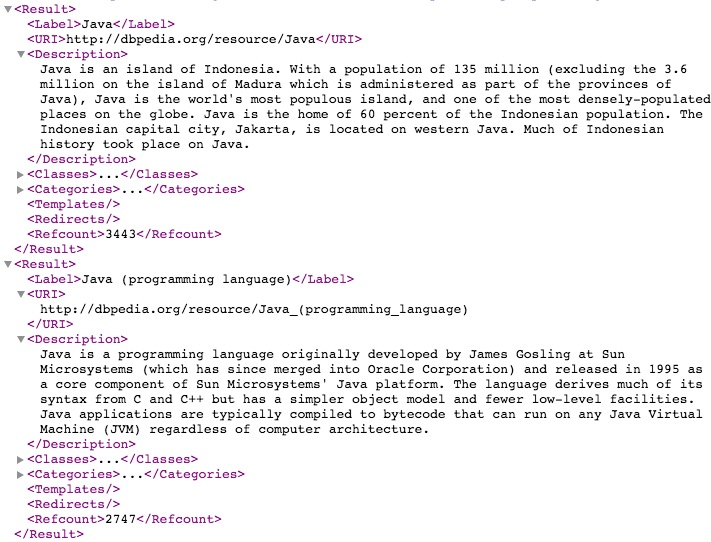
\includegraphics[width=5in]{chp6lookup.jpg}  
\caption{The example result of DBpedia lookup service for keyword \textit{java}}
\label{fig:chp6lookup} 
\end{figure}

In order to link \textit{java} to the correct DBpedia resource link. We compute the cosine similarity between the two descriptions from the two websites (StackOverflow and DBpedia) to solve the disambiguation problem. The  entire procedure is described as follows:

\begin{enumerate}
    \item{crawl the tag description from StackOverflow.}
    \item{retrieve DBpedia resources by the lookup service  }
    \item{compute the cosine distances between the description from StackOveflow and the description for each retrieved resource}
    \item{link the tag to the resource with the highest similarity}
\end{enumerate}


\subsection{Create graphs: retrieval potential links between resources}
After linking the tags to its corresponding DBpedia resources, we then perform several SPARQL queries to retrieve the potential relations among the resources found for each topic. 
\begin{itemize}
\item {Depth=1:} \\
select  ?relation \\
where\{ \\
\textit{ra} ?relation \textit{rb} . \\
\} 
\item{ Depth=2:} \\
select  ?r1, ?relation1, ?relation2 \\
where\{ \\
\textit{ra} ?relation1 ?r1 . \\
?r1 ?relation2 \textit{rb} .\\
\} 
\item{ Depth=3:} \\
select  ?r1, ?r2 ?relation1, ?relation2, ?relation3 \\
where\{ \\ 
 \textit{ra} ?relation1 ?r1 . \\
 ?r1 ?relation2 ?r2 .\\
 ?r2 ?relation3 \textit{rb} .\\
\} 
\end{itemize}
%TODO FAB: queries would be better presented as code.

Where, \textit{ra}, \textit{rb} are the resources for which we want to retrieve the potential relations. $?r1$, $?r2$, $?relation1$, $?relation2$, $?relation3$ are the potential relations and the intermediate resources. $Depth$ denotes the hops between the resources \textit{ra} and \textit{rb}. We vary this parameter by $1,2,3$. Figure \ref{fig:chp6resourcegraph} shown a retrieved graph for a linux related topic.
%TODO FAB: we have to explain why we don't use path expressions and what is the general idea behind these queries I propos the text below
To remain compatible with SPARQL 1.0 we did not use the path operator that would support a much synthetic way of writing these queries. The general idea behind these queries is to reconstruct a small connected graph around the detected resources for a topic in order to obtain a space where to analyze their relations.

\begin{figure}[htp]
\centering
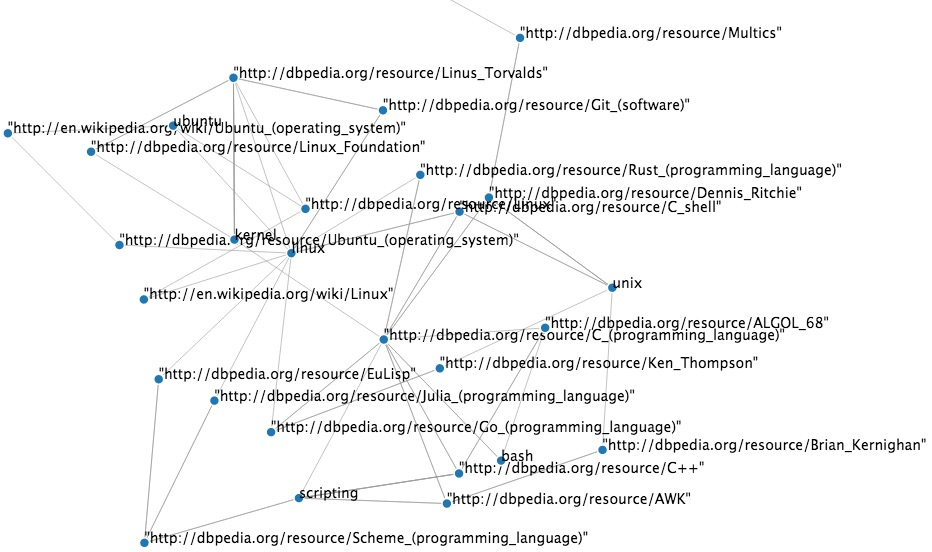
\includegraphics[width=5in]{chp6resourcegraph.jpg}  
\caption{The example graph structure for a linux topic}
\label{fig:chp6resourcegraph} 
\end{figure}

Once we have these relation graphs, we perform several graph algorithms to chose one or several resources as candidates to label the the bag of words of the topics. We mainly used the following algorithms/metrics:
\begin{itemize}
    \item {InDegree} \\
    In a directed graph, for a node, the number of head ends adjacent to a node is called the indegree of the node. 
    \item {Betweenness Centrality } \\
    It is an indicator of a node's centrality in a network. It is equal to the number of shortest paths from all vertices to all others that pass through that node.
    \item {Degree Centrality} \\
    It is defined as the number of links incident upon a node, which is equal to indegree plus outdegree for a directed graph.
    \item {Page Rank\cite{chp6page1999pagerank}}\\
    PageRank is an algorithm used by Google Search to rank websites in their search engine results. It can be applied on other kinds of graph to estimate the importance of the nodes.
    \item {Random} \\
    We just randomly choose one node from the graph.
    \item {Top tags} \\
    The topic modeling algorithm generates a topic-word distribution to indicate to what extent a word is related to a topic. By sorting words' corresponding probabilities, we can obtain a ranked word list for each topic, which are the top related words in each topic. A naive approach can use the first one or two tags to label each topic. 

\end{itemize}

\subsection{Experiments: A survey study}
In order to evaluate the performances of the different ways to generate labels we conducted user studies on the results. We designed two surveys for the user study. Table \ref{tab:chp6survey} shows the structure of the survey we used. For each survey, we listed 30 topics, half of them are from StackOverflow dataset, half of them are from Flickr dataset. The only difference for survey A and B is the linking (disambiguation) method. As mentioned in section \ref{sec:chp6secSolution}, we use both cosine similarity and babelfy to link tag with DBpedia resources. 

\begin{table}[htp]
\centering
\begin{tabular}{c|c|c}
\hline
             &  15 StackOverflow Topic& 15 Flickr Topic \\ \hline
    Survey A & Cosince Similairy & Babelfy\\ \hline  
    Survey B &  Babelfy          & Babelfy\\ \hline
\end{tabular}
\label{tab:chp6survey}
\end{table}


\subsubsection{Users' agreement}
We use Krippendorff’s Alpha\footnote{\url{https://en.wikipedia.org/wiki/Krippendorff's_alpha}} score to evaluate the degree of agreement among judges. The score indicates the homogeneity, or consensus, in the ratings given by judges. The score is always smaller than 1, $\alpha = 1 $ indicates the judges reach a perfect agreement and $\alpha =0 $ indicates the judges do not agree at all. When $\alpha <0 $ this means that judges reached a disagreement exceeding what can be expected by chance.  Figure \ref{fig:chp6alpha} illustrates the alpha score for 15 topics in each dataset and the average alpha score. We evaluate this score in three levels which correspond to the three sub figures. If we consider the top voted label as the best label, the first figure shows the agreement score among users. When we lower this limitation and consider the set of the top voted two labels as the best label, we can find that for most of the topics users could reach a good agreement. When we keep lowering this limitation and consider the top three voted labels as the best label, we can find there reach an excellent agreement. 



\begin{figure}[htp]
\centering
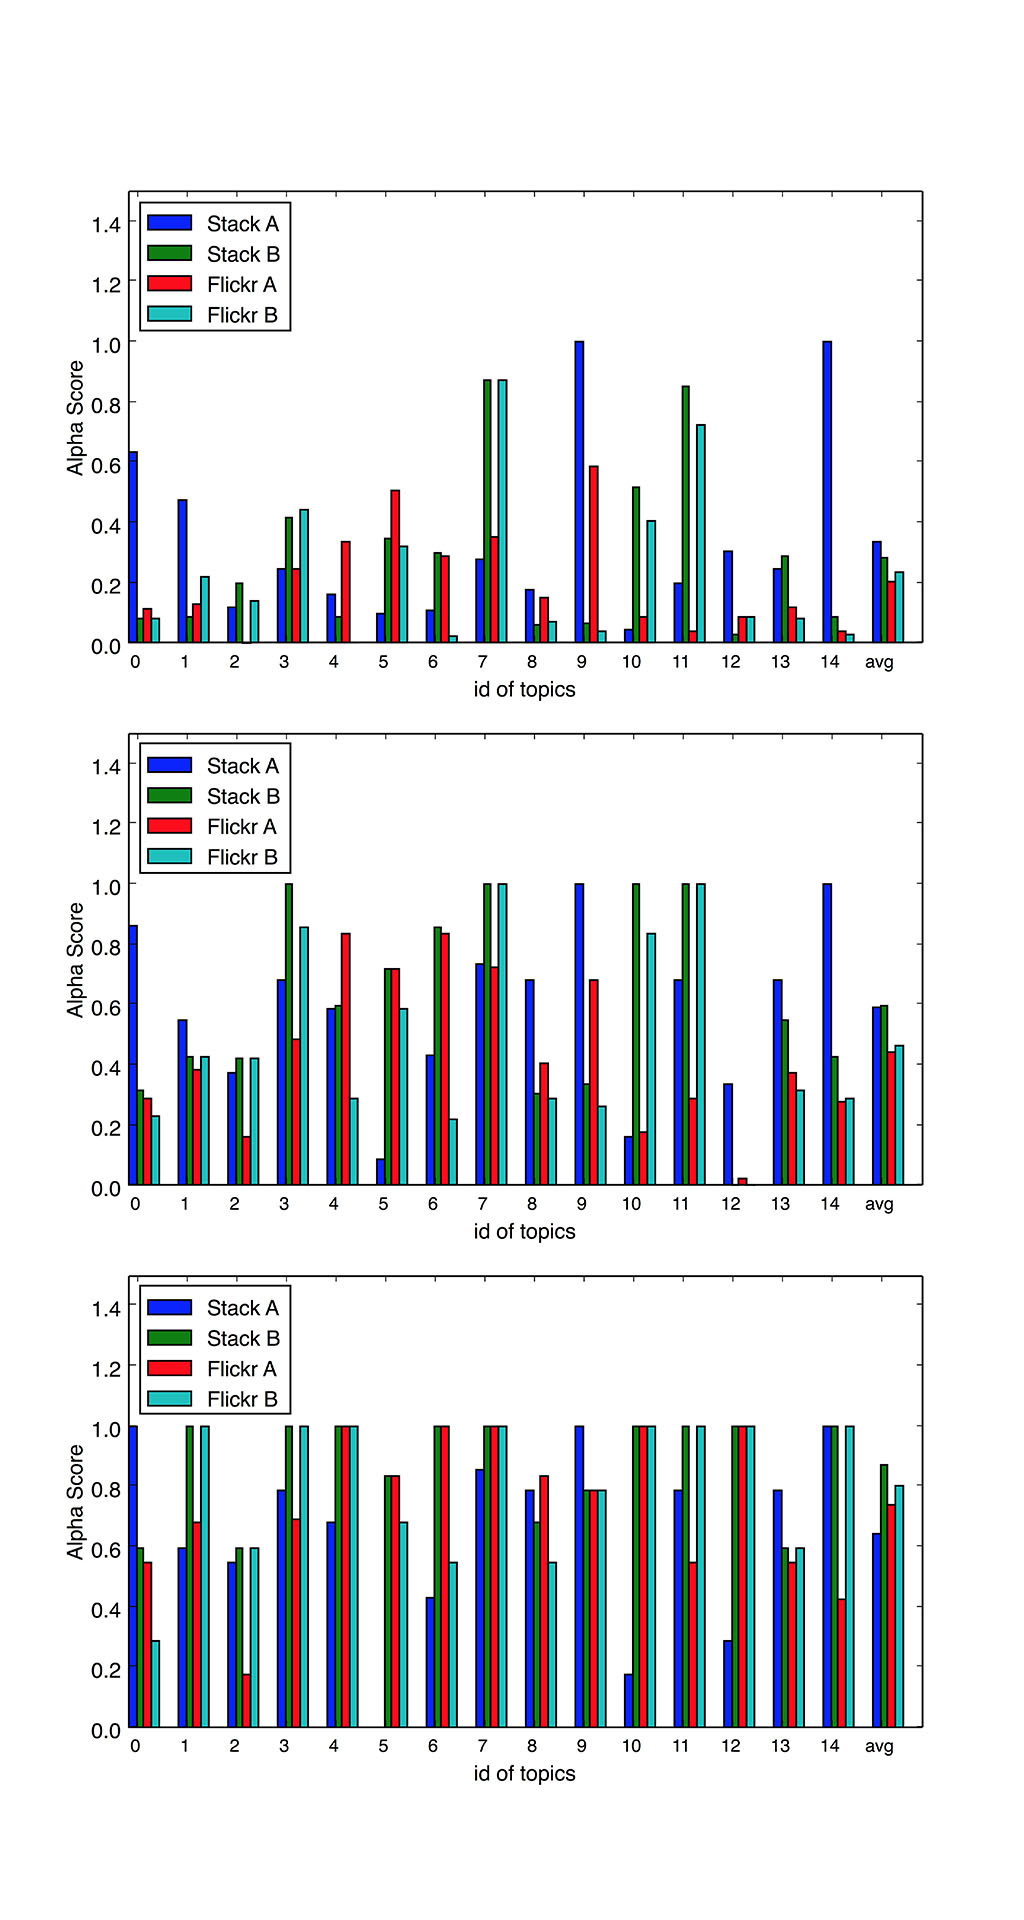
\includegraphics[width=5in]{chp6alpha.jpeg}  
\caption{}
\label{fig:chp6alpha} 
\end{figure}


In addition, we calculate the proportion of top voted labels. Figure \ref{fig:chp6top} shows the number of topics which top voted labels take a certain proportion. X-axis are the proportion, Y-axis are the number of topics. A data point ($50\%$,6) in the first sub figure means that there are 6 topics which first voted labels takes $50\%$ percent of all voted labels. A data point ($50\%$,6) in the second sub figure means that there are 6 topics which top two voted labels take $50\%$ percent of all voted labels. Similarly, A data point ($50\%$,6) in the third sub figure means that there are 6 topics which top three voted labels take $50\%$ percent of all voted labels. We can find that most of the labels chosen by judges are actually highly voted labels, which means all judges tend to agree on the top two or three labels.

\begin{figure}[htp]
\centering
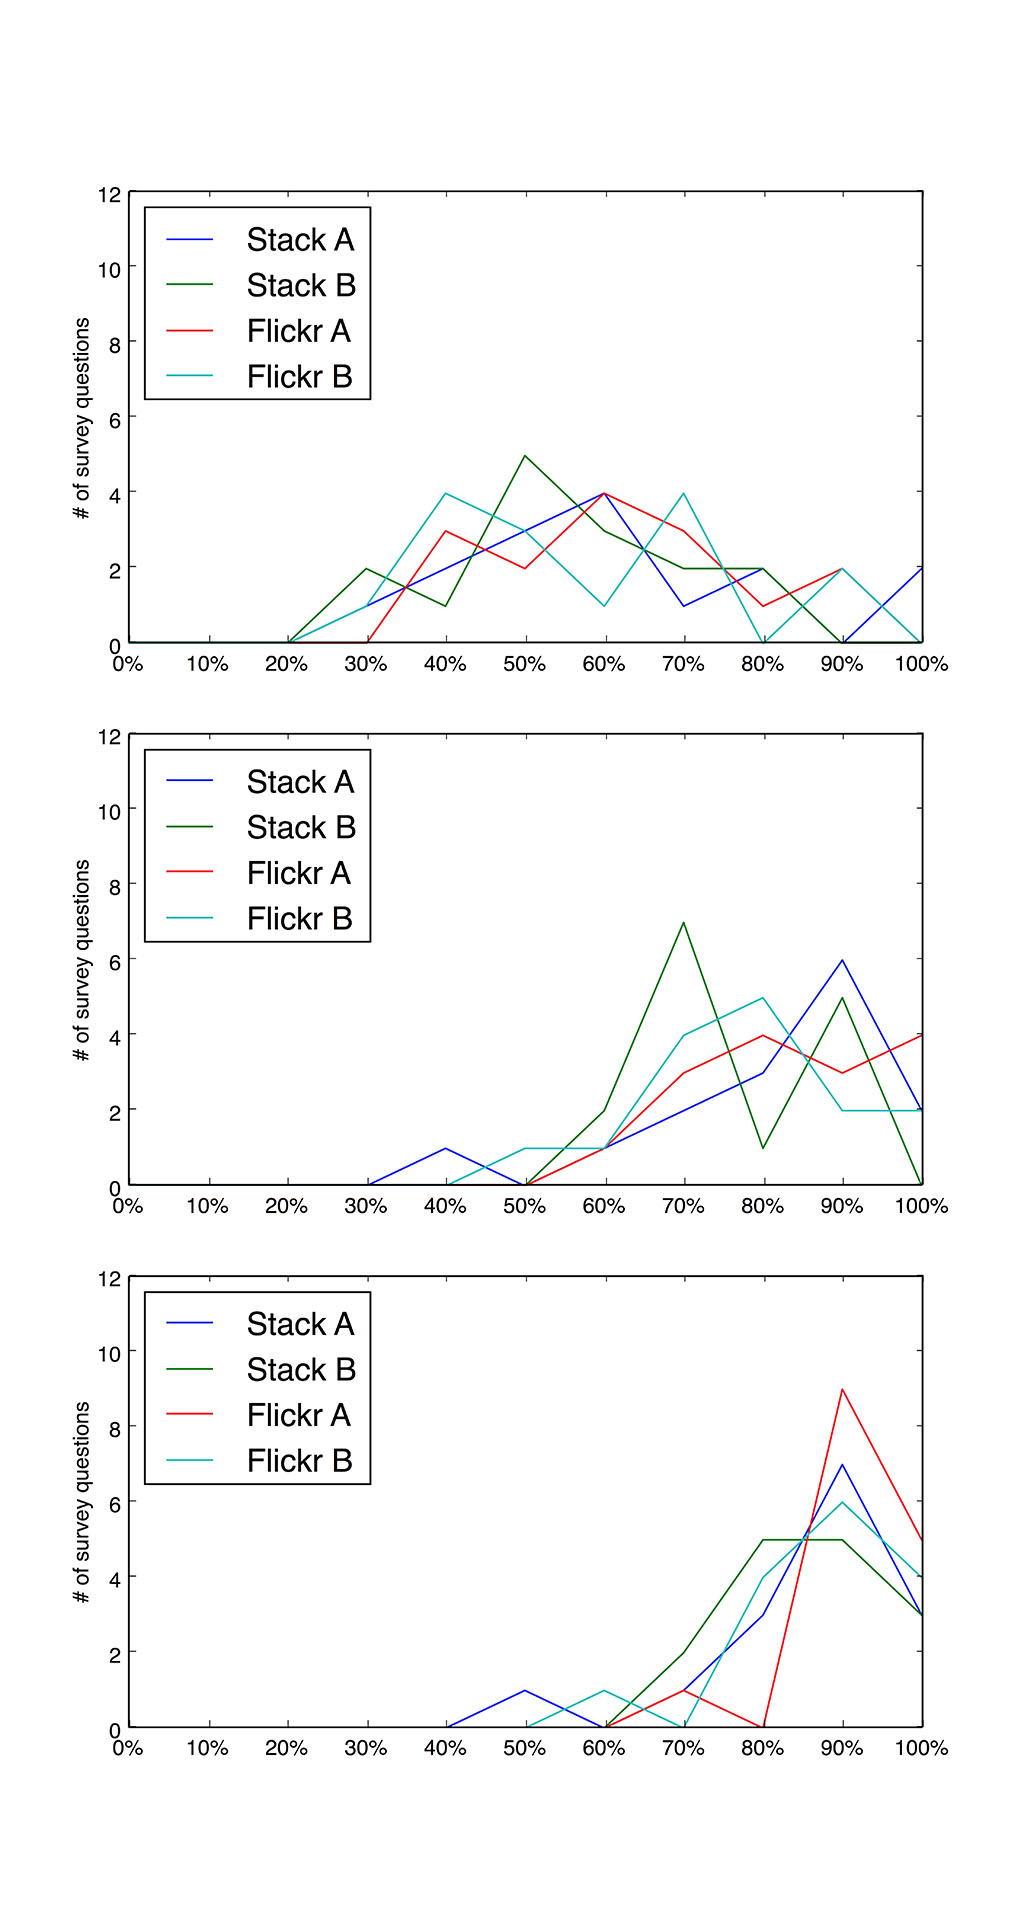
\includegraphics[width=5in]{chp6top.jpeg}  
\caption{}
\label{fig:chp6top} 
\end{figure}


\subsubsection{Quality evaluation: NDCG measurement}
We use NDCG metric to evaluate all the algorithms listed in Section \ref{sec:chp6secSolution}. The Normalized DCG (NDCG) is introduced to compare different ranking list. The value of NDCG is between 0.0 and 1.0. In our scenario, a NDCG@p value of 1.0 means detected interests and their order are totally the same as the labeled data until position \textit{p}, while a NDCG@p value of 0.0 means that the detected interests are completely different from the labeled data. For values between 0.0 to 1.0, it means that the detected interests are partially correct or ordered incorrectly. %It still 
Here, we evaluate NDCG@1, NDCG@2, and NDCG@3. The algorithm can generate a ranked label list. We sort the labels according to the number of votes from the survey as ideal ranking list. We also propose a method called \"Most+Top\". We created a label list by choosing a label which is the most recommended by all algorithms and labels from the \"Top tags\" algorithm. We can find that most of the algorithms can predict the good labels for a topic. Especially, if we consider giving two labels for a topic, our proposed method has very good results on all the datasets, which means for all the topics, the method can generate two good labels to represent the meaning of the topic.

\begin{figure}[htp]
\centering
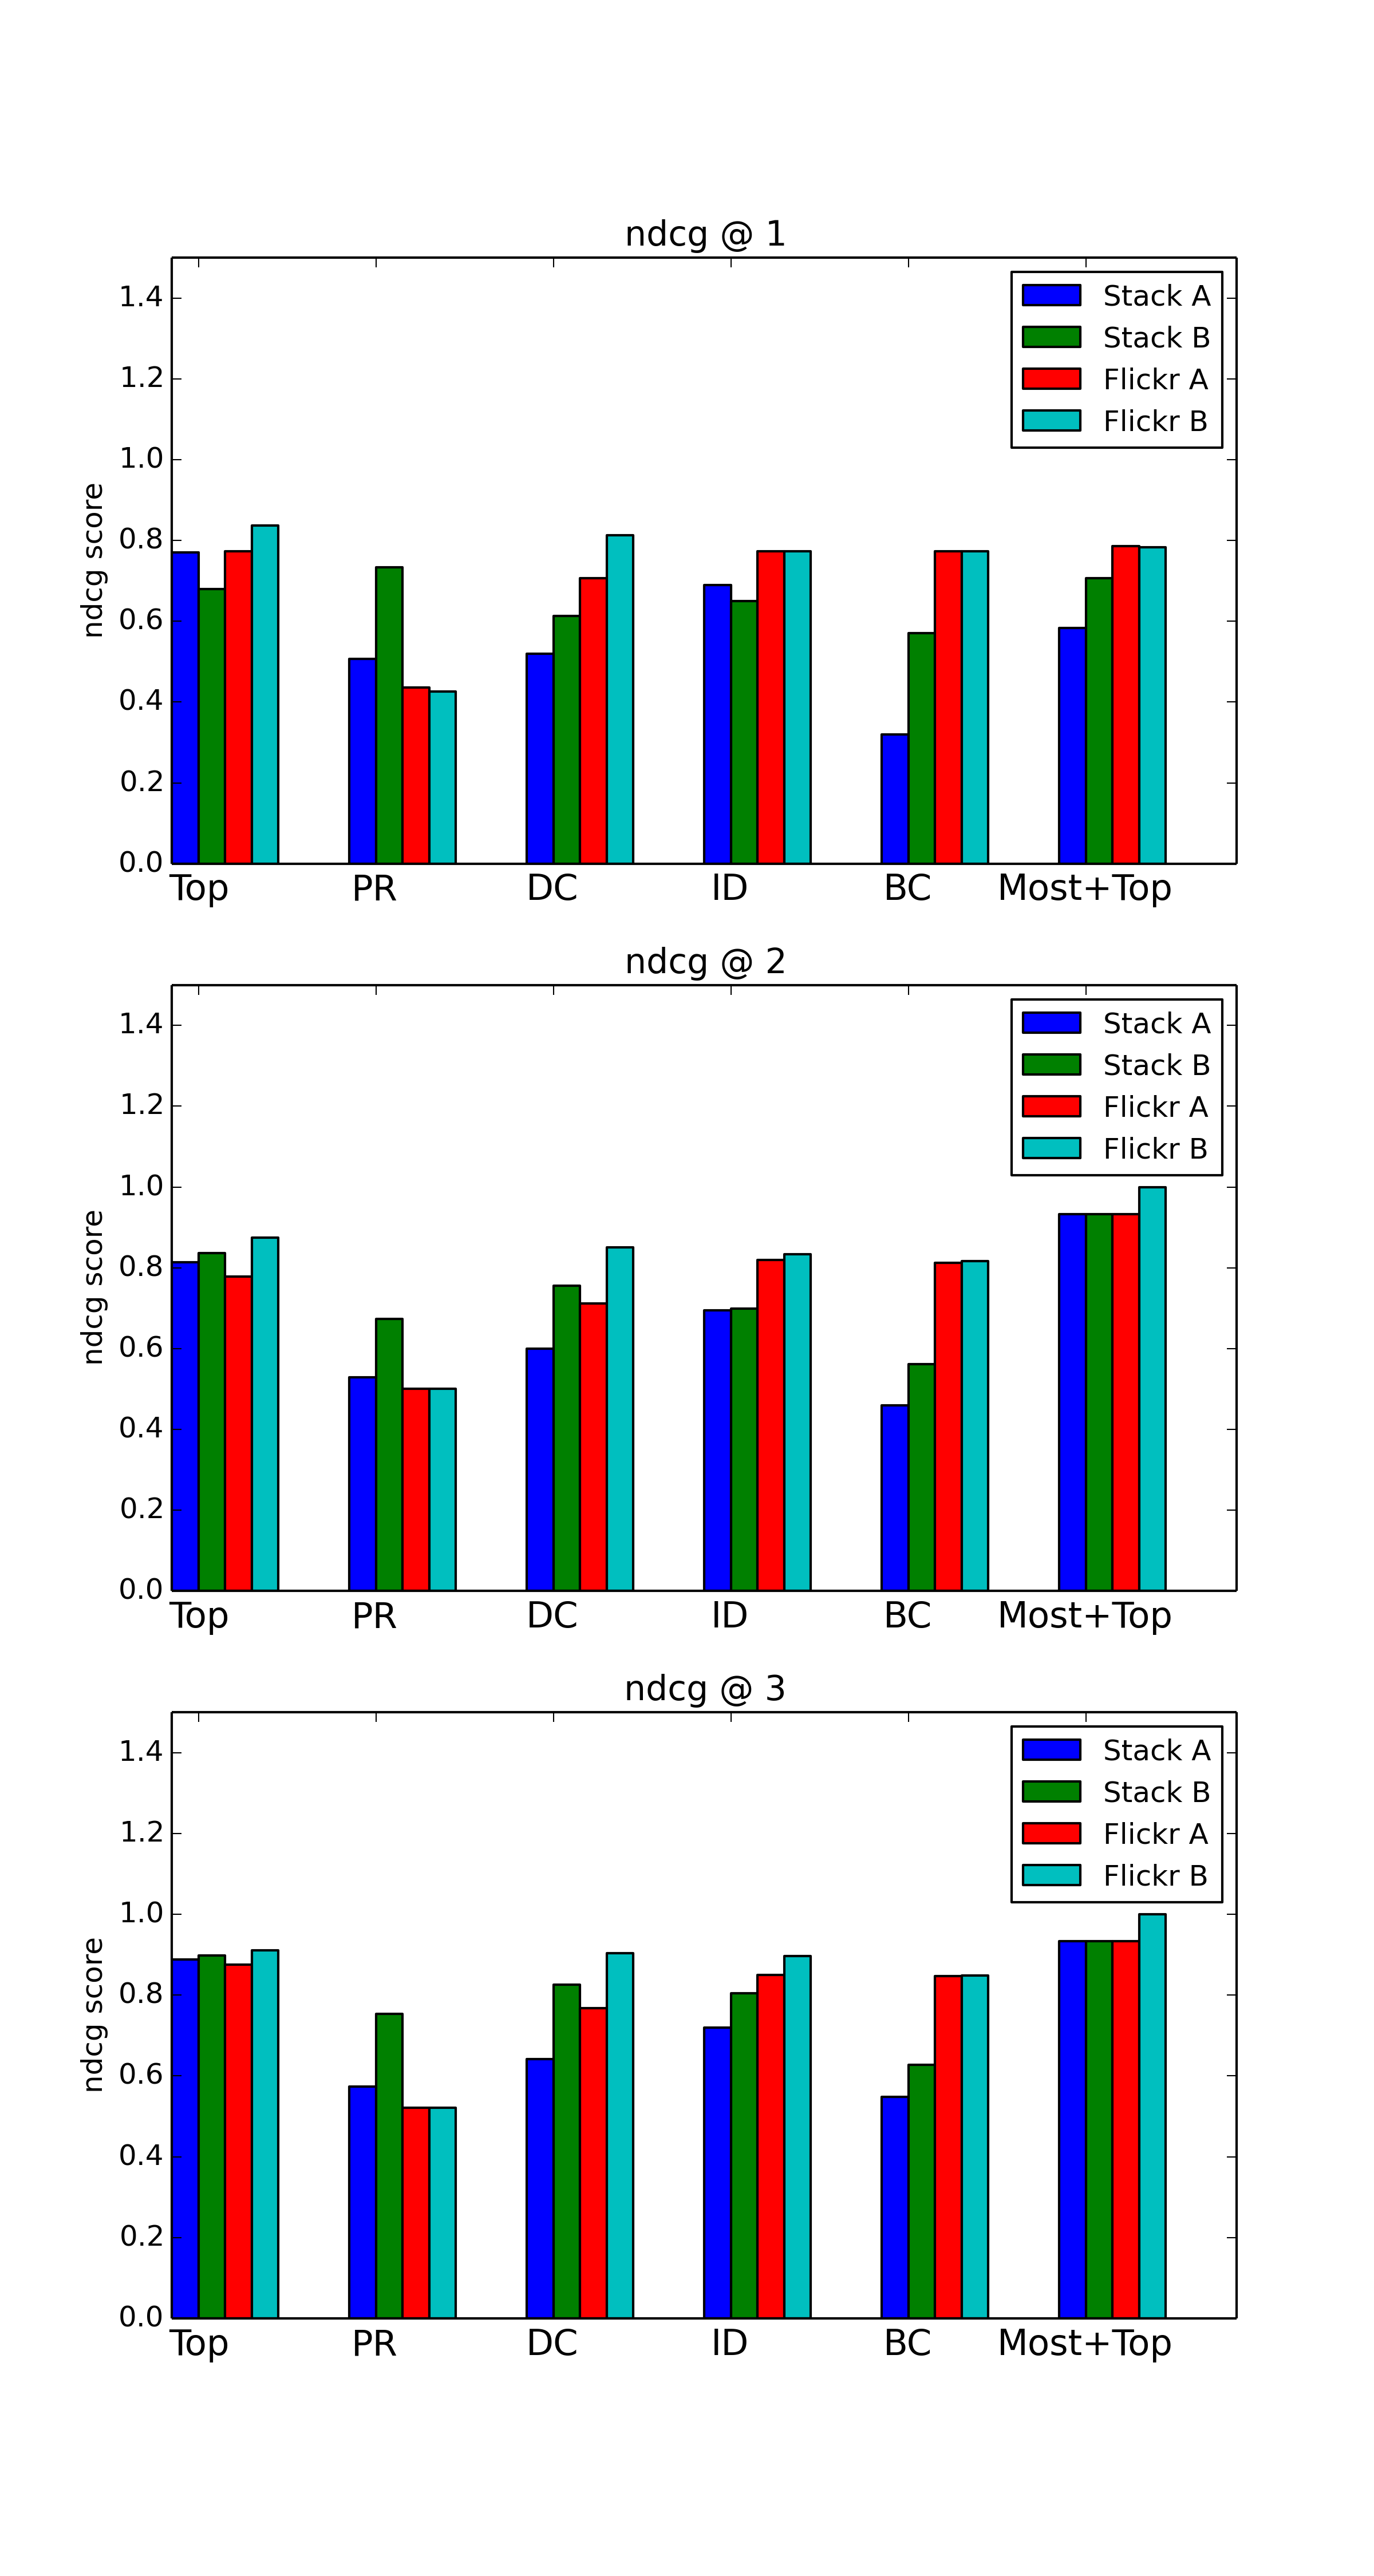
\includegraphics[width=5in]{chp6ndcg.jpeg}  
\caption{}
\label{fig:chp6ndcg} 
\end{figure}




\section{summary: represent a topic with labels}
In this chapter, we discussed how we used DBpedia as external knowledge to help choosing labels to turn bags of words into meaningful topics. From the user survey we found that users can reach a good agreement on a composite labels. Therefore, it is more reasonable to have more than one keyword to label the bag of words of atpoic. We also proposed a hybrid solution by combing results from different algorithms to generate composite labels to represent a topic. In the next chapter, we will focus on how to extract more sophisticated social information such as expertise, activity and trends.


\chapter{Temporal Topic Expertise Activity (TTEA)}
\doublespacing
\label{chap:ttea}
\minitoc


\section{Introduction: Mining expertise and temporal information}

Chapter \ref{chap:qasm} proposed a method to formalize the latent information in user-generated content. The key point was how to extract this information. Chapter \ref{chap:lda} introduced the use of the original LDA model to extract topics and communities. In this chapter, we extend the results of chapter \ref{chap:lda} to extract topic based expertise and topic based temporal knowledge.

Let us consider StackOverflow for an example of the problem we address. In StackOverflow, For instance, \textit{Alice} posts a question at \textit{08/11/2015}, and assigns it with the tags \{\textit{html}, \textit{css}, \textit{height}\}. Her question then gets \textit{30} votes, and \textit{Bob} gives an answer to this question at \textit{10/11/2015}, that gets a voting score of \textit{35}. Based on these original information, we want to propose a model to extract more latent information from it.

\subsection{Joint extraction of topics, trends, expertise, and activities}
The Temporal Topic Expertise Activity (TTEA) model we propose aims at jointly modeling topics, their trends, users' expertise, and their activities. 
More precisely, we aim at extracting the indicators listed in table \ref{tab:listofoutputs}. 

\begin{table}[htp] 
%\scriptsize
\caption{Output distributions of our model and their functionality}
\label{tab:listofoutputs}
\centering
\begin{tabular}{|c|c|}
\hline
\emph{Notation}  & \emph{Functionality of distribution} \\ \hline
$\theta_{uk}$ & detect a user's most interested topic \\ \hline
$\theta_{ku}$ & detect the most active users in a topic \\ \hline
$\theta_{kv}$/$\theta_{kw}$ & detect the most relevant tags/words in a topic \\ \hline
$\theta_{kt}$ & detect the trends of a topic \\ \hline
$\theta_{tk}$ & detect the most popular topic at point in time \\ \hline
%User,Time-Topic & detect a user's most interested topic at a point in time \\ \hline
$\theta_{ukt}$ & detect a user's activity pattern in a topic \\ \hline
$\theta_{uke}$ & detect a user's most expertise topic\\ \hline
%User,Exp-Topic & detect a user's most experted topic \\ \hline
\end{tabular}
\end{table}

\subsection{Fundamental Notions in Defining a TTEA}
Let us now define the basic notions later used in the description of TTEA:

\textbf{Topic} ($\theta_{kw}/\theta_{kv}$): A bag of words or tags which are closely related. Words are the content of questions or answers, tags are attached to questions. For example, the topic-tag distribution \textit{Database}:\{{\textit{mysql}: 0.5, \textit{sql}: 0.3, \textit{query}: 0.2\}. expresses that topic \textit{Database} is related to tags \textit{mysql}, \textit{sql}, and \textit{query}. 

\textbf{User Topical Interest}($\theta_{uk}$): A user is interested in different topics with different levels. For example, the user-topic distribution \textit{Alice}:\{{\textit{Database}: 0.8, \textit{Java}: 0.2\} expresses that \textit{Alice} prefers to answer questions related to \textit{Database}, but rather not about \textit{Java}. 

\textbf{User Topical Activity}($\theta_{ku}$):  Different users are interested in the same topic with different levels. For example, the topic-user distribution \textit{Database}:\{{\textit{Alice}: 0.8, \textit{Bob}: 0.2\} expresses that \textit{Alice} prefers to answer question related to \textit{Database}, while \textit{Bob} is not willing to contribute answers to it.

\textbf{Topic Trend}($\theta_{kt}$): A topic is popular at different points in time with different levels. For example,the topic-time distribution \textit{Database}:\{{\textit{May/2013}: 0.2, \textit{June/2013}: 0.3, \textit{July/2013}: 0.5\} expresses that the topic \textit{Database} is increasingly popular.% while the topic \textit{java} remains stable.

\textbf{Topic Temporal Activity}($\theta_{tk}$): Topics are active at a point in time with different levels. For example, the time-topic distribution \textit{Sept/2013}:\{{\textit{Ios}: 0.8, \textit{Database}: 0.2\} expresses that \textit{ios} related questions are popular in Sept. 2013, while \textit{Database} related questions are not specially popular.

\textbf{User Topic Temporal Dynamics}($\theta_{ukt}$): A user is interested in different topics at different points in time with different levels. For example, the topic-time distribution for \textit{Alice} \textit{ios}:\{{\textit{May/2013}: 0.2, \textit{June/2013}: 0.3, \textit{July/2013}: 0.5\} expresses that \textit{Alice}'s interest to topic \textit{ios} is increasing.


\textbf{User Topical Expertise}($\theta_{uke}$): A user has expertise in different topics with different levels. For example, the topic-expertise distribution for \textit{Alice} \textit{ios}:\{{\textit{High}: 0.2, \textit{Medium}: 0.7, \textit{Low}: 0.1\} expresses that \textit{Alice}'s expertise on topic \textit{ios} is probably in medium level.

\section{TTEA Model and Computation}
\subsection{TTEA Probabilistic Graphical Model}

%%updated wi2016
The TTEA model we propose is based on LDA. Figure \ref{fig:tteamodel} represents it using the plate notation. The original LDA model is in red with dotted line style, and our extension is in blue with solid line style. Let $u_i \in \{1, 2,..., U\}$ be the set of users, $p_i \in \{1, 2,..., P\}$ the set of answer posts, which are generated by these users, $w_i \in \{1, 2,..., W\}$ the set of words in answers posts, $ta_i \in \{1, 2,..., Ta\}$ the set of tags which are attached to posts, $v_i \in \{1, 2,..., V\}$ the set of votes for each answer posts, $ti_i \in \{1, 2,..., Ti\}$ the set of points in time which could be months or days depending on the requirements, and $z_i \in \{1, 2,..., K\}$ the set of topics for the posts. Here, $U$, $P$, $W$, $Ta$, $V$ ,$Ti$ and $K$ denote the total number of users, posts, words, tags, votes, points in time, and topics. $\alpha$, $\beta$, $\delta$, $\gamma$, $\eta$, and $\lambda$ are Dirichlet priors. The notation and description of distributions $\theta_{uk}$, $\theta_{kv}$, $\theta_{kw}$, $\theta_{kt}$, and $\theta_{uke}$ are listed in Table \ref{tab:listofoutputs}.

\begin{figure}
\centering
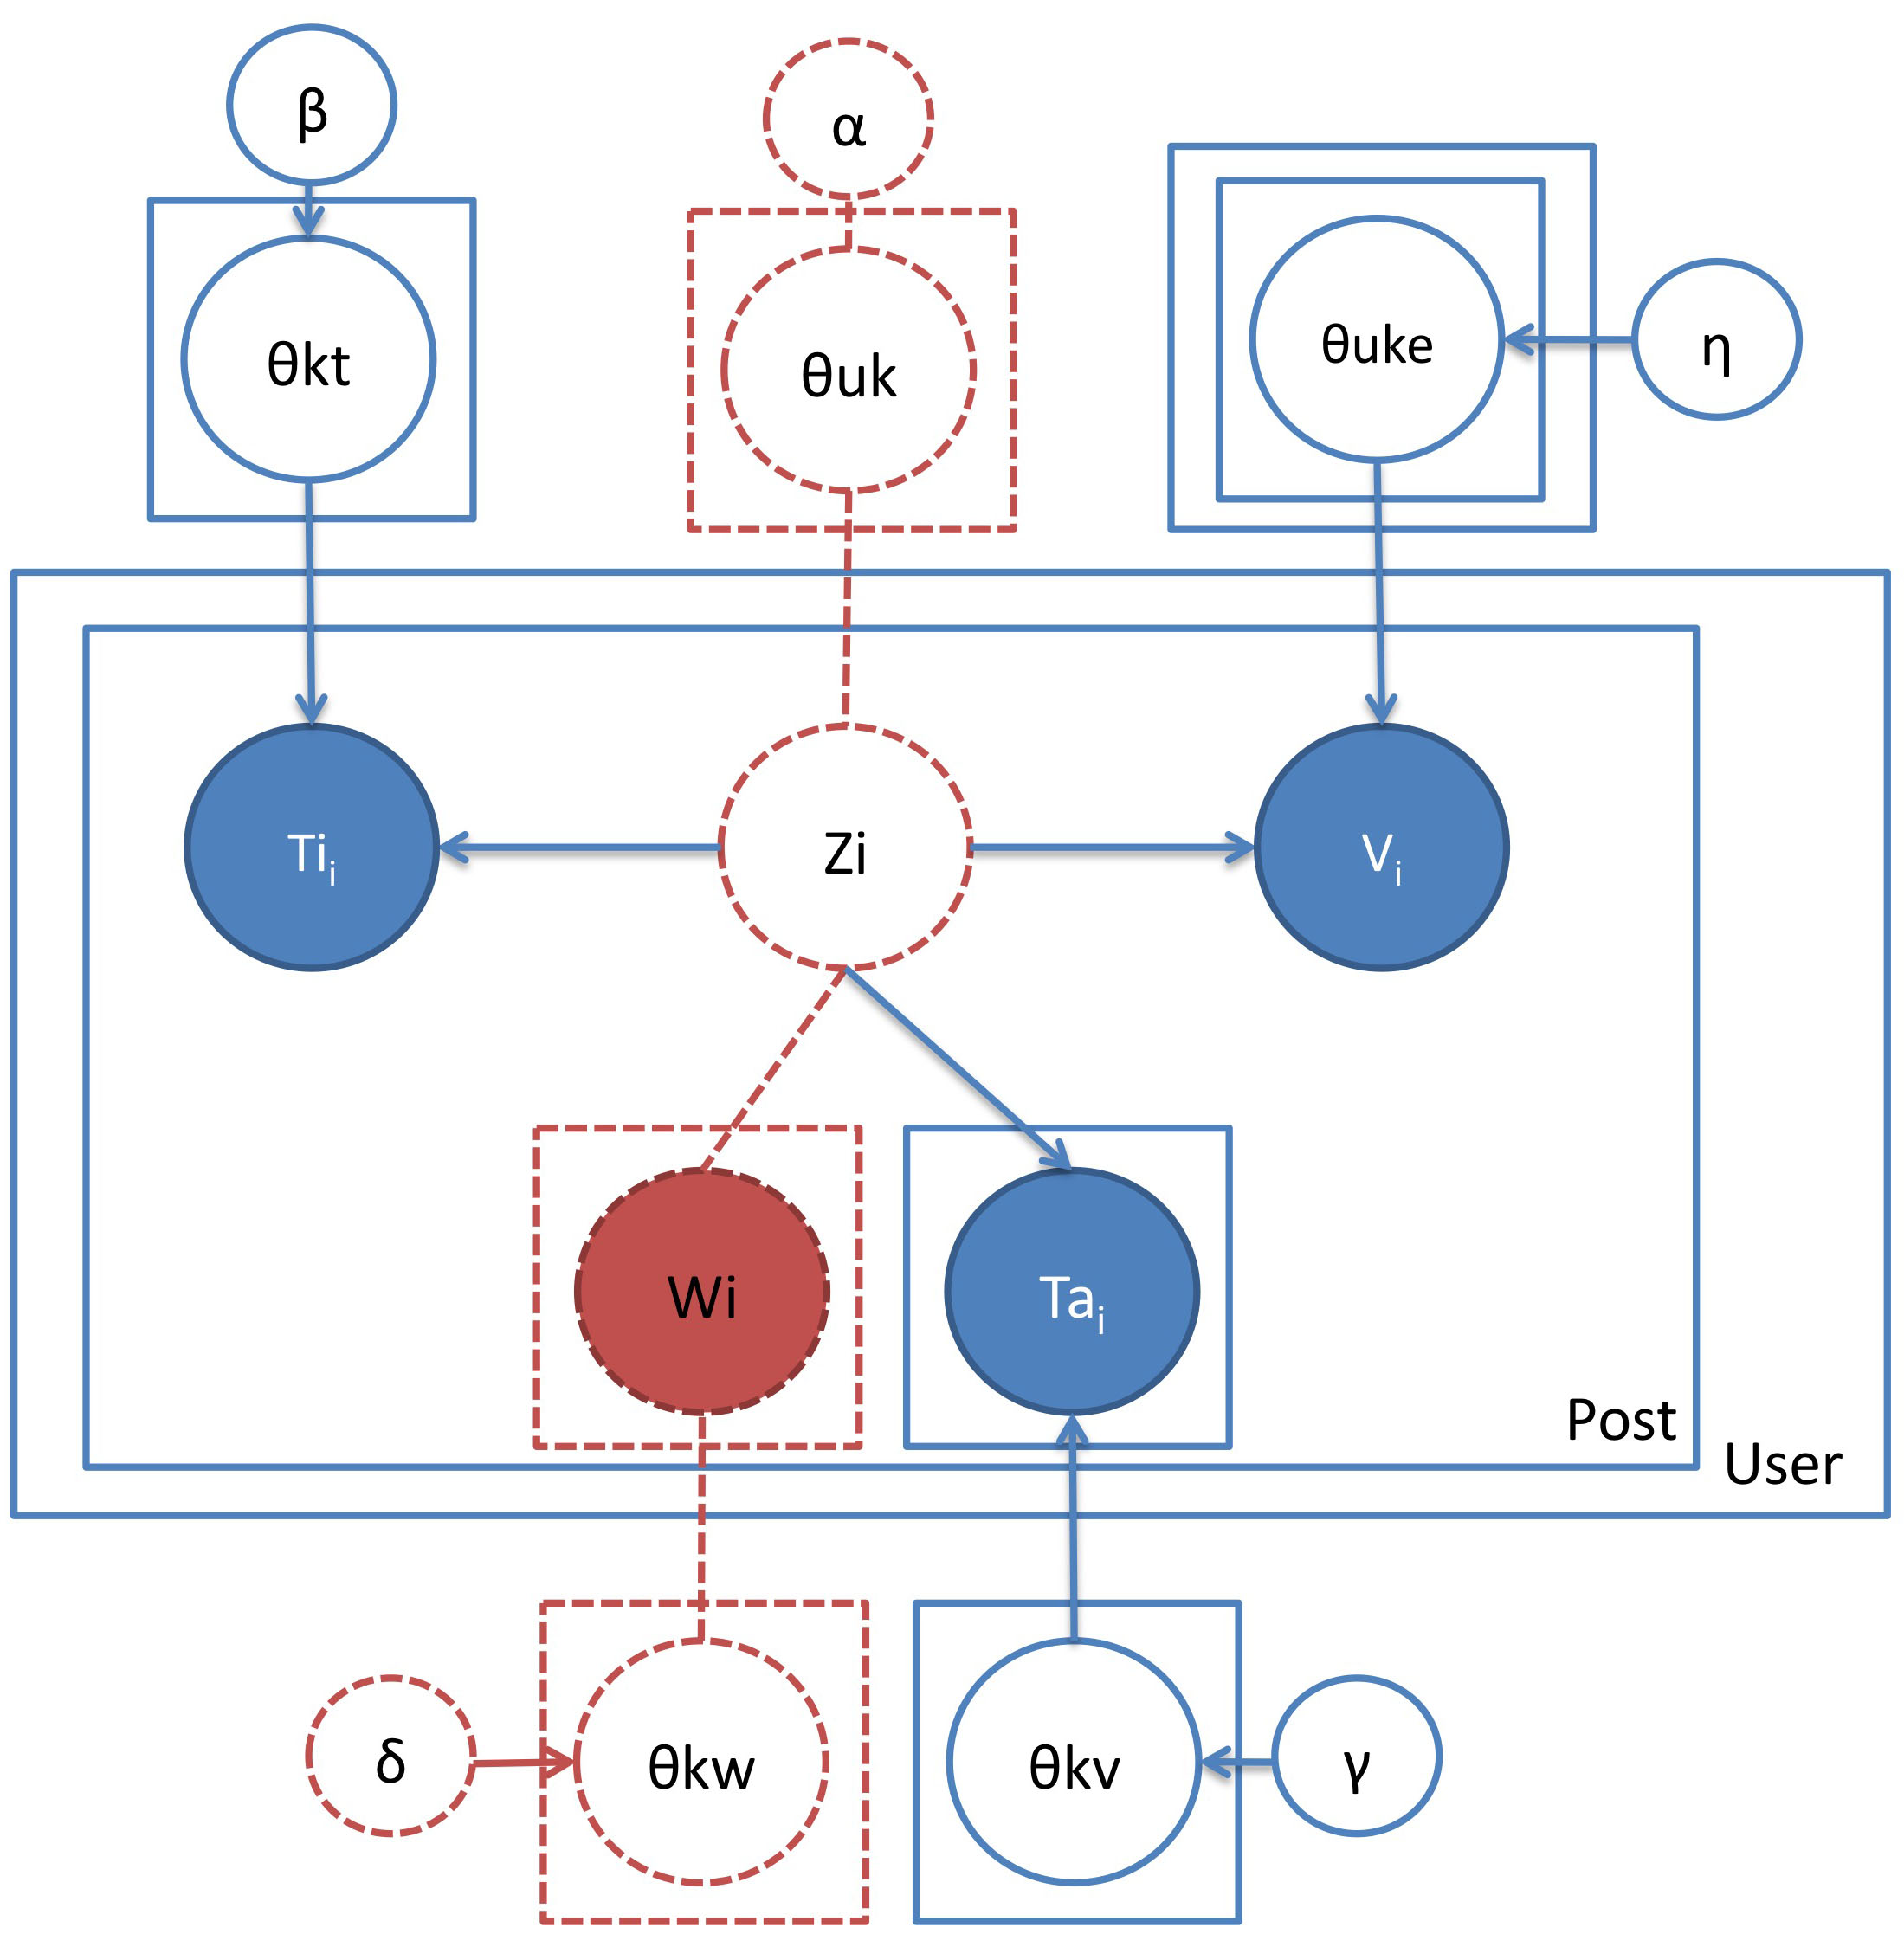
\includegraphics[ width=5.1in]{tteafinal.jpg}  
\caption{TTEA Model}
\label{fig:tteamodel} 
\end{figure}

%TODO Cath : would the following paragraph rather come in a previous chapter?
%NOTE Zide here to indicate the reasons and the differences of ttea model compared with other model.
Contrary to \cite{blei2003latent} who applied LDA model on long documents such as news articles and assumed that each word has a latent topic, we assume in TTEA that each answer post has one topic: like in other social media with short contributions, e.g. Twitter, an answer post is normally short, each answer post is therefore suitable to be assigned with one single latent topic, and all the words in that post are considered to be generated by this topic. Some work\cite{chp7zhao2011comparing}\cite{chp7diao2012finding} on microblog also made this assumptions.

For expertise modeling, we do not use votes directly because (a) the vote scores are sparse and noncontinuous, and (b) it is not reasonable to tell that a vote score $55$ is better than a vote score $50$ if the vote score are ranging from $0$ to $3000$.  Since the vote scores' counts distribution follows a log distribution\cite{yang2013cqarank}, we use the logarithmic value of vote score, and separate them into several expertise levels, which is one of the parameters: the expertise level.

For temporal modeling, like \cite{wang2006topics} \cite{hu2014user}, we use time stamps directly. In order to model time at different levels, we simply split time stamps into different parts (month, day, and hour) and use them separately depending on the demands.

%TODO in the following section some aspects have already been explained in previous chapters, you must at least indicate the aspects that remain the same and ifferentiate the new ones.
%DONE, this part is the description of generative process. It is not the same as problem define.

%TODO Cath I think that you must point out the similarities with you rformalisation in chapter 4 and 5.
%NOTE, Zide. the difference is  shown in the fig ttea model. the following generative process is just a  description the fig7.1 in a more detailed a orgranized way.

The generative process of TTEA model is :
Let us consider a user $u$ who wants to answer a question. She first selects a topic $k$ according to her user-topic distribution $\theta_{uk}$. Then she writes an answer post $p$. The words of $p$ are generated from topic $k$'s topic-word distribution $\theta_{kw}$. Since only the questions have tags, we consider the answers automatically acquire all the tags of the question they respond to. Then the answer post $p$ acquires its tags according to the topic-tag distribution $\theta_{kv}$ of topic $k$. Meanwhile, the answer post $p$ gets a time-stamp $ti$ according to the topic-time distribution $\theta_{kt}$ of topic $k$.
This procedure is described as follows:


\begin{algorithm}%[htp]
\begin{algorithmic}[1]
\label{algo:algotopic}
\State \textit{/*The generative process*/}
\For { the u-th user $u$ \textbf{in} $U$ }
\State draw user topic distribution $\theta_{uk}$ $\sim$ Dir( $\alpha$) 
\EndFor
\For { the k-th topic $k$ \textbf{in} $K$ } 
\State draw topic tag distribution $\theta_{kv}$ $\sim$ Dir($\gamma$)
\State draw topic word distribution $\theta_{kw}$ $\sim$ Dir($\delta$)
\State draw topic time distribution $\theta_{kt}$ $\sim$ Dir($\beta$)
\EndFor
\For { the u-th user $u$ \textit{in} $U$ }
\For { the k-th topic $k$ \textit{in} $K$ }
\State draw user topic expertise distribution $\theta_{uke}$ $\sim$ Dir($\eta$) 
\EndFor
\EndFor
\For {the u-th user $u$ \textit{in} $U$}
\For {the n-th q\&a post $p$ \textit{in} $P$}
\State draw topic $z$ $\sim$ Multi($\theta_{uk}$)
\State draw time point $t$ $\sim$ Multi($\theta_{kt}$)
\State draw expertise level $v$ $\sim$ Multi($\theta_{uke}$) 
\For {the i-th word $w$ \textit{in} $W$ }
\State draw word $w$ $\sim$ Multi($\theta_{kw}$) 
\EndFor
\For {the j-th tag $ta$ \textit{in} $Ta$ } 
\State draw tag $t$ $\sim$ Multi($\theta_{kv}$)
\EndFor
\EndFor
\end{algorithmic}
\end{algorithm}

\subsection{TTEA Model Inference: using collapsed gibbs Sampling}

Like \cite{hu2014user}, we use the collapsed Gibbs Sampling algorithm \cite{griffiths2004finding} to sample the hidden variable $z$, based on which the unknown probabilities \{$\theta_{uk}$, $\theta_{kv}$, $\theta_{kw}$, $\theta_{kt}$,  and $\theta_{uke}$ \}%part of them, need to modified
can be estimated. % For simplicity we set the hyper parameters to \{$\alpha$, $\beta$, $\delta$, $\gamma$, $\eta$, $\lambda$\}.

%TODO cite the papers on how to tune the hyper parameters.
%DONE, this has been put into  the experiment.


The TTEA inference process is as follows.
We iteratively sample the topic indicator $z_i$ for each answer post $p_i$ according to equation \ref{eq:sample}. The intuition behind this equation is to combine two parts of possibilities: (1) the possibilities to generate the topic indicator $z_i$ and (2) the possibilities generated by the topic indicator $z_i$. Besides, the intuition behind each part in Equation \ref{eq:sample} are corresponding to Equation \ref{eq:uk}, \ref{eq:kv}, \ref{eq:kw}, \ref{eq:kt} and \ref{eq:uke}. As explained before, each question/answer post will have one topic assignment. 


\begin{equation}
\begin{split}
p(z_i=k & | z_{\neg i}, \textbf{U}, \textbf{Ti}, \textbf{Ta}, \textbf{W}  ) \\
&\propto   \frac{ C_{u,\neg i}^k + \alpha_1 }{ \sum_{k=1}^K C_{u,\neg i}^k+ K* \alpha_1} \\
&\cdot \frac { \prod_{ta=1}^{Ta} \prod_{q=0}^{C_{ta}-1} ( C_{k,\neg i}^{ta} +q+\gamma) } { \prod_{p=0}^{\sum C_{ta} -1} \sum_{ta=1}^{Ta} (C_{k,\neg i}^v + p + Ta*\gamma  ) } \\
&\cdot \frac { \prod_{w=1}^{W} \prod_{s=0}^{C_w-1} ( C_{k,\neg i}^{w} +s+\delta) } { \prod_{t=0}^{\sum C_{w} -1} \sum_{w=1}^W (C_{k,\neg i}^w + t + W*\delta  ) } \\
&\cdot \frac{ C_{k,\neg i}^{ti} + \beta  }{\sum_{ti=1}^{Ti} C_{k,\neg i}^{ti} + Ti*\beta} \\
&\cdot \frac{ C_{u,k,\neg i}^{e} + \eta }{\sum_{e=1}^{E} C_{u,k,\neg i}^{e} + E * \eta}\\
\end{split}
\label{eq:sample}
\end{equation}

\noindent
where $\neg i$ enforces that all the counters used are calculated with the answer post $p_i$ excluded. $C_{u,\neg i}^k$ is the number of posts by user $u$ assigned to topic $k$, $C_{ta}$ is the number of tags $ta$ in $p_i$, therefore, $\sum C_{ta}$ is the total number of tags in $p_i$, $C_{k,\neg i}^{ta}$ is the number of tags $ta$ assigned to topic $k$. Similarly, $C_{w}$ is the number of words $w$ in $p_i$, $\sum C_{w}$ is the number of words in $p_i$, $C_{k,\neg i}^{w}$ is the number of words $w$ assigned to topic $k$. $C_{k,\neg i}^{ti}$ is the number of posts assigned to topic $k$ and posted at time $ti$. $C_{u,k,\neg i}^{e}$ is the number of posts which are assigned to topic $k$ and got a vote score in the range of expertise level $e$.

Then, with the result of the Gibbs sampling algorithm, we can make the following parameter estimation:
\begin{equation}\scriptsize
\theta_{uk}=\frac{ C_u^k + \alpha }{ \sum_{k=1}^K C_u^k+ K* \alpha} 
%\text{user-topic distribution}\\
\label{eq:uk}
\end{equation}
\begin{equation}\scriptsize
\theta_{kv}=\frac{ C_k^{ta} + \gamma }{ \sum_{ta=1}^{Ta} C_k^{ta}+ Ta* \gamma}
%\;\;\;\;\;\;\;\;\;\;\;\;\;\;\;\
%\text{topic-tag distribution}
\label{eq:kv}
\end{equation}
\begin{equation}\scriptsize
\theta_{kw}=\frac{ C_k^w + \delta }{ \sum_{w=1}^W C_k^w+ W* \delta}
%\;\;\;\;\;\;\;\;\;\;\;\;\;\;\;\
%\text{topic-word distribution}
\label{eq:kw}
\end{equation}
\begin{equation}\scriptsize
\theta_{kt}=\frac{ C_k^{ti} + \beta }{ \sum_{ti=1}^{Ti} C_k^{ti}+ Ti* \beta}
%\;\;\;\;\;\;\;\;\;\;\;\;\;\;\;
%\text{topic-time distribution}
\label{eq:kt}
\end{equation}
\begin{equation}\scriptsize
\theta_{uke}=\frac{ C_{u,k}^e + \eta }{ \sum_{e=1}^E C_{u,k}^e+ E* \eta} 
%\;\;\;\;\;\;\;\;\;\;\;\;\;\;\;
%\text{user-topic-expertise distribution}
\label{eq:uke}
\end{equation}


\subsection{Post Processing: Extracting activity indicators}\label{sec:detailed}

The previous model can only generate the distributions \{$\theta_{uk}$, $\theta_{kv}$, $\theta_{kw}$, $\theta_{kt}$, and $\theta_{uke}$ \}. To generate the other distributions, e.g. $\theta_{ku}$, $\theta_{tk}$ and $\theat_{ukt}$, we directly use the sample results at each iteration and keep recording the corresponding counters. Therefore, $C_k^u$ is the number of posts assigned to topic $k$ and posted by user $u$, $C_{ti}^k$ is the number of posts posted at time $ti$ and assigned to topic $k$. $C_{u,k}^{ti}$ is the number of posts by user $u$, assigned to topic $k$ and posted at time $ti$.
% $C_{u,k}^e$ is the number of posts by user $u$ assigned to topic $k$ with an expertise level $e$. We use the same method to estimate the probabilities.
Then, we estimate $\theta_{ku}$, $\theta_{tk}$, $\theat_{ukt}$ according to the following equations:
\begin{equation}%\scriptsize
\theta_{ku}=\frac{ C_k^u + \alpha_2 }{ \sum_{u=1}^U C_k^u+ U* \alpha_2} 
%\;\;\;\;\;\;\;\;\;\;\;\;\;\;\;\;\;\;\;\;\;\;\;\;\;\;
%\text{topic-user distribution}
\end{equation}
\begin{equation}%\scriptsize
\theta_{tk}=\frac{ C_{ti}^{k} + \beta_1 }{ \sum_{k=1}^{K} C_{ti}^{k}+ K* \beta_1}
%\;\;\;\;\;\;\;\;\;\;\;\;\;\;\;\;\;\;\;\;\;\;\;\;\;
%\text{time-topic distribution}
\end{equation}
\begin{equation}%\scriptsize
\theta_{ukt}=\frac{ C_{u,k}^{ti} + \lambda }{ \sum_{ti=1}^T C_{u,k}^{ti}+ T* \lambda} 
%%\;\;\;\;\;\;\;\;\;\;\;\;\;\;\;\;\;\;\;\;\;
%\text{user-topic-time distribution}
\end{equation}


%TODO Cath you may split this section into 2 sections
%note Zide, yes, split into 2 section.
\section{TTEA Model Experiments and Evaluation on StackOverflow data}\label{sec:TTEAexperiment}

\subsection{Basic statistic of StackOverflow Dataset: an overview}


We conducted experiments on a dataset from StackOverflow. This site releases its whole content every three month. For our experiments, we used the data dump from July 2008 to March 2013. 

Table \ref{tab:basicinfo} and figure \ref{fig:basicstat} provide basic statistics on the dataset.
\begin{table}[htp]
\caption{Basic statistics on the dataset}
\label{tab:basicinfo}
\centering
\begin{tabular}{|c|c|}
\hline
number of tags & 32,379\\ \hline
number of questions & 4,592,961 \\ \hline
number of users asking questions & 833,041 \\ \hline
number of users providing answers & 8,585,113\\ \hline
number of questions having accepted answers & 2,808,825\\ \hline

\end{tabular}
\end{table}

\begin{figure}
\centering
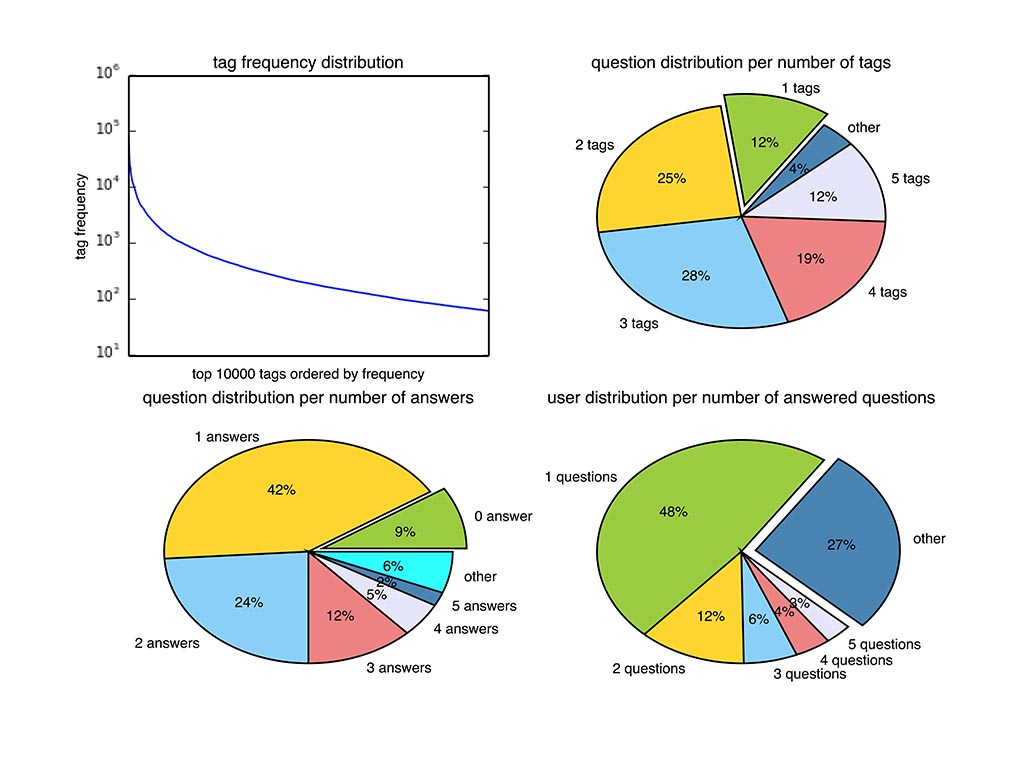
\includegraphics[ width=5in]{output.jpg}  
\caption{Basic perspectives of the dataset}
\label{fig:basicstat} 
\end{figure}

%TODO: include as many figures, charts, etc. as you can.
%fig: number of user answered questions.
%fig: number of user for each questions.
%fig: distribution of tags per questions.
%fig: tag frequency

%TBD
%fig: title_length vs num_answer. 
%fig: heatmap of question and answer. 


Here are some general observations about the dataset: 
\begin{itemize}
    \item nearly half of the questions do not have accepted answers;
    \item nearly half of the questions only have one answer and it maybe inadequate;
    \item more than a third of the questions only have one or two tags;
    \item nearly half of the users only answer one question so question routing and incentives are important problems;
    \item nearly 10\% percent of the questions do not have answers.
\end{itemize}



\subsection{Experiment Dataset and Compared Methods}
In the experiments described in Chapter \ref{chap:ttd}, we only used a part of this data set (from 2008 to 2009), and we mainly focused on several co-answer graph. Besides, we also labeled this small dataset.
Considering the large volume of the dataset over 3 years, the processing time is extremely long. \cite{chp7ldatimecomplexity} shows that the complexity of each iteration of the Gibbs sampling for LDA is linear with the number of topic and the number of documents, which is $O(KN)$.  
In the experiments described in this chapter and aiming at evaluating the effectiveness of our model, in order to simplify the processing, we chose two continuous months from the dataset (From Jan 2011 to June 2011, from July 2011 to Jan 2012), with no bias to the selections.

To evaluate the effectiveness of our model, we compared it with several related works:  
\begin{itemize}
\item{TTEA} is our method for modeling user, topic, temporal and expertise in Q\&A sites. Besides, we also model activities by adding virtual nodes. We can generate the user-topic distribution and topic-activity distribution simultaneously. 
\item{TEM}: \cite{yang2013cqarank} proposed a model for user, topic and expertise in Q\&A sites. It integrates a Gaussian Mixture Model to model expertise, which is time consuming. We simplify this process by directly modeling votes information. Besides, it does not model temporal information and user topic activities. 
\item{UQA}: \cite{guo2008tapping} proposed a User-Question-Answer model for modeling users and topics in Q\&A  sites. In certain Q\&A  sites, questions have category information which have proved to be very useful. The category in their model is similar to tags in TTEA model and TEM model. However we allow multiple tags for each posts while they can only set a single category.
\item{GrosToT}: \cite{hu2014user} proposed a User-Group-Topic-Time model for modeling users, groups, topics and time in social media sites. It introduces a group level between user and topic compared with other models. It does not directly generate user-topic distribution, so we compute it with the user-group distribution and group-topic distribution.% $\theta_{uk}$ so we compute it by $\theta_{uk} \propto \sum_{g=1}^{G} \theta_{ug} * \theta_{gk}$.
\item{LDA}: based on \cite{blei2003latent} we apply LDA model to create a User-Topic-Post model for modeling users and topics. It can generate the user-topic distribution and topic-words distribution.
%\begin{equation}\scriptsize
%\end{equation}

\end{itemize}

%TODO: the evaluation and its description must be different from the TTD one and emphasize the time aspect that was added.
%DONE explained below.

We choose the same number of topics K=\textit{30} as \cite{Chang:2013} and the same number of expertises E=\textit{10} as \cite{yang2013cqarank}, which have proved to be a reasonable setting for the Stackoverflow dataset. We empiricaly set Dirichlet hyper parameters $\alpha_1$=$\alpha_2$=50/K, $\beta_1$=$\beta_2$=0.01, $\delta$=$\lambda$=$\eta$=0.01, $\gamma$=0.001 according to suggestions in \cite{griffiths2004finding}. 


\subsection{Performance of Topic Extraction: perplexity score}


In Chapter \ref{chap:ttd}, we have evaluated the perplexity score for both TTD and LDA model. The evaluation aimed to check wether our model can have a similar or better performance on topic extraction than the much more complicated probabilistic graphical model. In this section, we re-evaluate the perplexity score only among those probabilistic graphical models as our TTEA model is a probabilistic graphical model. Besides, we evaluate on a much larger dataset compared with Chapter \ref{chap:ttd}.

Table \ref{tab:toptagsp} and Table \ref{tab:topwordsp} show the top tags and words detected by our model. We use again the Perplexity~\cite{blei2003latent} metric as a quantitative way to measure the performance of topic extraction.

We include in our training dataset all the posts in the two months from August $1^{st}$ 2011 to October $1^{st}$ 2011, from users having more than 80 posts (as in \cite{yang2013cqarank}).
The resulting training dataset contains 87516 Q\&A posts by 674 users. For data preprocessing, we tokenized the texts and removed the stop words. For the testing dataset, we used all the posts of the same set of users than the training data but this time from October $1^{th}$ 2011 to January $1^{th}$ 2012. So training and testing datasets have no overlap but concern the same community. We varied the number of topics: 10, 30, 50, and 100. 
For a testing set of M posts, $N_i$ denotes the number of words in the $i^{th}$ post and the Perplexity score is computed according to equation \ref{eq:getperplexity}.
%\begin{small}
\begin{equation} %\scriptsize
  Perplexity(D_{test})=exp\left\{-\frac{\sum_{i=1}^{M}\log p(W_i)}{\sum_{i=1}^{M}N_i}\right\}
\label{eq:getperplexity}
\end{equation}
%\end{small}
where $p(W_i)$ is the probability of the words in the test document $d_i$. In our model, $p(W_i)$ is computed according to equation \ref{eq:getprobabilitywords}.:% $P(W_i)=\sum_{k}\theta_{u_ik}\prod_{w} \theta_{kw_i}$:
\begin{equation}%\scriptsize
  P(W_i)=\sum_{k}\theta_{u_ik}\prod_{w} \theta_{kw_i}
\label{eq:getprobabilitywords}
\end{equation}
\begin{figure}[htp]
\centering
%\epsfig{file=fly.eps, height=1in, width=1in}
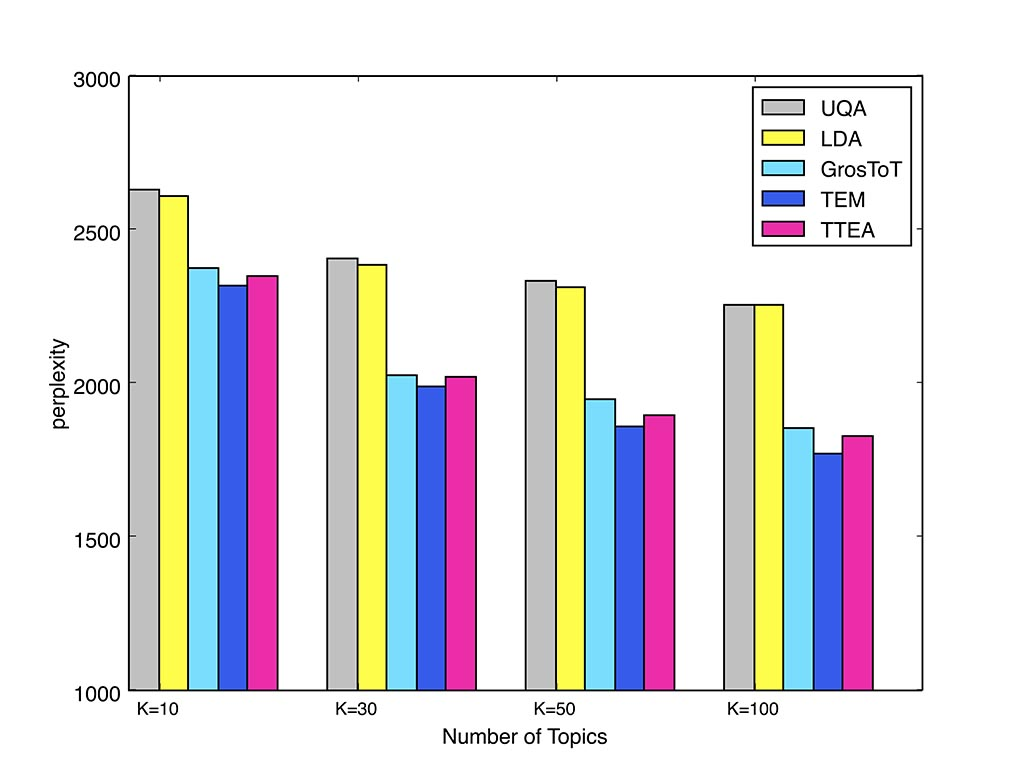
\includegraphics[width=5in]{perplexityv2.jpg}  % use this if you use "pdflatex"
\caption{Comparison of topic extraction performances}
\label{fig:perplexity} % Fig.2
\end{figure}



\begin{sidewaystable}
%\begin{table*}[htp]
%\begin{table}[!t]
\caption{Top tags for different topics generated by the TTEA model}
\label{tab:toptagsp}
\centering
\scriptsize
%\begin{tabular}{p{34pt}p{34pt}p{34pt}p{34pt}p{34pt}p{34pt}p{34pt}p{34pt}p{34pt}p{34pt}}
\begin{tabular}{cccccccccc}
\hline
Topic 1& Topic 2& Topic 3& Topic 4 & Topic 5 & Topic 6& Topic 7 & Topic 8 &Topic 9 & Topic 10\\
\hline
php&c##&iphone&c++&javascript&android&sql&java&jquery&git \\ 
xslt&.net&objective-c&c&jquery&java&mysql&spring&javascript&svn \\ 
xml&linq&ios&pointers&php&android-layout&sql-server&eclipse&html&version-control \\ 
xpath&generics&xcode&templates&ajax&listview&php&jsp&css&github \\ 
mysql&asp.net&cocoa-touch&stl&html&activity&query&.htaccess&jquery-selectors&mercurial \\ 
html&vb.net&ipad&arrays&json&android-intent&tsql&servlets&jquery-ui&eclipse \\ 
arrays&c#-4.0&uitableview&vector&asp.net&sqlite&sql-server-2008&jsf&dom&tortoisesvn \\ 
jquery&reflection&iphone-sdk-4.0&string&jquery-ajax&layout&join&mod-rewrite&php&linux \\ 
javascript&entity-framework&cocoa&function&forms&android-widget&select&maven&javascript-events&clearcase \\ 
foreach&list&xcode4&c++11&asp.net-mvc-3&xml&sql-server-2005&apache&ajax&ssh \\
\hline
\end{tabular}
%\end{table*}
\end{sidewaystable}

\begin{sidewaystable}
%\begin{table*}[htp]
%\begin{table}[!t]
\caption{Top words for different topics generated by the TTEA model}
\label{tab:topwordsp}
\centering
%\scriptsize
%\begin{tabular}{p{34pt}p{34pt}p{34pt}p{34pt}p{34pt}p{34pt}p{34pt}p{34pt}p{34pt}p{34pt}}
\begin{tabular}{cccccccccc}
\hline
Topic 1& Topic 2& Topic 3& Topic 4 & Topic 5 & Topic 6& Topic 7 & Topic 8 &Topic 9 & Topic 10\\
\hline
xsl&aspx&view&std&jquery&android&select&html&jquery&git \\ 
td&msdn&reference&const&ajax&activity&join&java&div&branch \\ 
tr&microsoft&nsstring&pointer&script&html&group&file&click&commit \\ 
template&library&apple&char&javascript&view&order&spring&element&file \\ 
select&select&html&template&page&developer&table&jar&event&svn \\ 
row&linq&library&vector&html&intent&key&apache&input&repo \\ 
echo&system&documentation&operator&form&reference&count&eclipse&document&repository \\ 
table&dictionary&developer&compiler&url&layout&row&docs&text&files \\ 
match&ienumerable&ios&memory&document&try&inner&servlet&html&master \\ 
node&expression&release&struct&json&button&query&web&api&github \\ 
\hline
\end{tabular}
%\end{table*}
\end{sidewaystable}

Figure \ref{fig:perplexity} shows the perplexity results for our TTEA method and other state-of-the-art methods. 
TTEA is almost as good as TEM. But TEM integrates a Gaussian Mixture Model, which is time consuming. The training process of TEM is nearly three times longer than the other models.



\section{Task Evaluation: Question routing and Expert recommendation} 

\subsection{Question Routing: recommending new questions to potential users}
\label{sec:qrouting}
\cite{Chang09} suggested that topic models should focus on evaluations on real-world task performance rather than on optimizing likelihood-based measures. So, in addition to the perplexity-based evaluation, we used the results of TTEA to perform real-world tasks and we evaluated them. This is described in this subsection and the following ones.
In this section we focus on question routing: given a question $q$ and a set of users $U$, the task is to rank all these users by their interests to answer question $q$.
We score each user $u$ by considering the similarity between his topics of interest and the topics of the question ($Sim(u,q)$). The intuition behind equation \ref{eq:simquestion} is that the more a user is interested in the topic of a question, the more likely he is to provide an answer to that question.
\begin{equation}
Sim(u,q) = (1 -JS(\theta_{uk},\theta_{qk}))
\label{eq:simquestion}
\end{equation}
where $\theta_{uk}$ is the user topic interest distribution, $\theta_{qk}$ is the question topic distribution, and JS(.) is the Jensen-Shannon divergence distance. We obtain $\theta_{uk}$ directly from model results. For $\theta_{qk}$, we apply equation \ref{eq:thetaqk}.
\begin{equation}
\begin{split}
\theta{q,k} &\propto p(k|w_q,t_q,u) \\
           &=p(k|u)p(w_q|k)p(t_q|k) \\
           &= \theta{uk} \sum_{w_i \in w_q} \theta_{kw_i} \sum_{t_i \in t_q} \theta_{kv_i} 
\end{split}
\label{eq:thetaqk}
\end{equation}
where $w_q$ and $t_q$ are the sets of all the words and tags in question $q$ and $\theta{kw}$, $\theta{kv}$ are the topic-word distribution and topic-tag distribution obtained directly from the model result. Then for question $q$, we compute the $Sim$ score for user set $U$ and rank them in decreasing order. % of the $Sim$ score.


We used all the posts from July $1^{th}$ 2011 to October $1^{th}$ 2011 from users having more than 50 Q\&A posts for the training dataset. Rather than using the threshold of 80 post like in \cite{yang2013cqarank}, we empirically set it to 50 posts to get enough users for recommendation. 
The resulting training set contains 297881 posts by 2555 users. For the testing dataset, we used all the questions posted by the same set of users as in the training set but this time from October $1^{th}$ 2011 to January $1^{th}$ 2012. Therefore the training and testing datasets have no overlaps. We removed testing questions which have no, or only one, answer. The resulting test dataset contains 6044 questions, 18077 answers and 7888 involved users. 

We also chose another period for this experiment. Besides, we varied the number of topics by $15$ and $50$, we varied the filter limit by $40$ and $80$. The experimental results are shown in section \ref{sec:parasetting}.

In order to evaluate different models, we considered precision at position N ( Precision@N or simply P@N) and recall at position N (Recal@N or simply R@N), which are widely used measures in the Information Retrieval community. Let $R_q$ be the recommendations of users for a question $q$ and $U_q$ be the actual set of users who posted for question $q$. Then Precision@N is defined in equation \ref{eq:precisionatn} and Recal@N is defined in equation \ref{eq:recallatn}.
\begin{equation}%\scriptsize
 P@N = \frac{1}{|Q|}\sum_{q \in Q}\frac{|R_q \cap U_q|}{|R_q|}
\label{eq:precisionatn}
 \end{equation}
 
 \begin{equation}%\scriptsize
 R@N = \frac{1}{|Q|}\sum_{q \in Q}\frac{|R_q \cap U_q|}{|U_q|}
\label{eq:recallatn}
 \end{equation}

\noindent
where $Q$ is the set of testing questions. Like in \cite{Chang:2013}, we use the Matching Set Count (MSC) which is defined in equation \ref{eq:matchingsetcount}. The idea is to count the number of successful recommendations, i.e., for which at least one of the recommended users answered the question.
 \begin{equation}%\scriptsize
 MSC@N = \frac{1}{|Q|}\sum_{q \in Q} 1[R_q \cap U_q \neq \emptyset]
\label{eq:matchingsetcount}
 \end{equation}
 where $1[condition]$ is equal to 1 if $condition$ is true, otherwise 0. 

\begin{sidewaystable}
% \begin{table*}[htp]
\caption{Question Routing experiments, Random denotes that we randomly recommend users for the test questions.}
\label{tab:qrouting}
%\scriptsize
\centering
\begin{tabular}{|c|c|c|c|c|c|c|c|c|c|c|c|c|}
\hline
 & p@5    &p@10    &p@20   & p@30 &r@5 & r@10 & r@20 &r@30 & msc@5 & msc@10 &msc @20 &msc@30  \\ \hline


%average 5 times, 
TTEA&0.024&0.019&0.015&0.013&0.045&0.072&0.111&0.142&0.112&0.178&0.269&0.339 \\ \hline
TTEA-ACT&0.028&\textbf{0.022}&\textbf{0.017}&\textbf{0.014}&0.052&\textbf{0.083}&\textbf{0.127}&\textbf{0.159}&0.134&\textbf{0.209}&\textbf{0.313}&\textbf{0.382} \\ \hline
TEM&0.024&0.019&0.015&0.013&0.045&0.073&0.114&0.146&0.114&0.179&0.275&0.344 \\ \hline
TEM-ACT&0.029&\textbf{0.023}&\textbf{0.018}&\textbf{0.015}&0.054&\textbf{0.084}&\textbf{0.129}&\textbf{0.162}&0.137&\textbf{0.210}&\textbf{0.315}&\textbf{0.388} \\ \hline
UQA&\textbf{0.030}&0.019&0.012&0.010&\textbf{0.062}&0.075&0.095&0.112&\textbf{0.149}&0.179&0.224&0.261 \\ \hline
GROSTOT&0.027&0.017&0.011&0.009&0.055&0.067&0.085&0.099&0.134&0.164&0.204&0.236 \\ \hline
RANDOM&0.001&0.001&0.001&0.001&0.001&0.002&0.005&0.007&0.003&0.007&0.013&0.019 \\ \hline
\end{tabular}
%\end{table*}
\end{sidewaystable}

In addition, our model can capture activity and we believe this information improves question routing. The intuition is that even if a user has a high $Sim$ score for a question, the less he is active, the less likely he is to provide an answer to that question. Therefore, we defined a score $SimAct$ to combine both topic similarity and activity level as shown in equation \ref{eq:newscore}, where $Act(u,q)$ is the computed activity score for user $u$ to question $q$. A high value of the $Act$ score indicates a high probability of activity on a question. We use TTEA to denote the method using only the similarity information, that is to say, ranking users by $Sim$ score. We use TTEA-ACT to denote the method using both similarity and activity, that is to say, ranking users by $SimAct$ score. We also integrated our activity model to the TEM model  and we refer to it as TEM-ACT. 
\begin{equation}
\begin{split}
SimAct(u,q) &= (1 -JS(\theta_{uk},\theta_{qk}))* Act(u,q) \\
         &= (1 -JS(\theta_{uk},\theta_{qk}))* \sum_{k=1}^{K} \theta_{qk} * \theta_{ku}
\end{split}
\label{eq:newscore}
\end{equation} 


Table \ref{tab:qrouting} shows the results. We ran the experiments five times and listed the average scores. Our observations can be summerized as follows:
\begin{itemize}
    \item UQA and GROSTOT perform the better when the number of recommended users is small, and TTEA and TEM begin to outperform UQA and GROSTOT when the number of recommended users is large;
    \item TTEA-ACT shows the best performances compared with the baseline competitors;
    \item both TTEA-ACT and TEM-ACT perform better than the other models. The activity modeling is a generic method that could improve the performance not only of our model, but also of other models although here we only show the result for the activity model with TEM as an example;
    \item even if TEM or TEM-ACT perform better than our model they remain again time consuming. Experiments show that the training process takes around 3$\sim$4 times longer compared to our model
\end{itemize}   


\subsection{Experiment Parameter Sensitivity Analysis}
\label{sec:parasetting}

%TODO Cath I do not understand the title of this subsection
%Note zide. during the experiments, i use some parameters , such as the number of topic, fliter threshold.etc. here I just vary these parameters to check the result again.

%TODO Cath Start by explaining what you will focus on in this subsection.
%DONE, check the following.
The above experiments have shown the effectiveness of our model. However, we use some arbitrary parameters, we vary these settings and conduct the experiment again in this section.
\begin{itemize}
    \item we use posts from another period of time.
    \item we vary topic number by 15, 50. We use 30 in the previous experiments.
    \item we vary the filter threshold by 40, 80. This threshold equal to 60 means that ignoring a user if she has less than 60 posts. We use 60 in the previous experiments.
\end{itemize}

For the training dataset, we used all the posts in a three months period, from January $1^{th}$ 2011 to March $31^{th}$ 2011, from users having at least 50 q\&a posts, rather than 80 posts like \cite{yang2013cqarank}, in order to get enough users for recommendations. The training set contains 371181 posts by 3123 users. For the testing dataset, we used all the questions posted by the same set of users as in the training set, but this time from April $1^{th}$ 2011 to June $31^{th}$ 2011. Therefore the training and testing datasets have no overlaps. We removed questions with no or only one answer. The resulting test dataset contains 9048 questions, 27870 answers and 10147 users. 
Table \ref{tab:qrouting123456} shows the question routing results. We can still find that TTEA-ACT outperforms all the baseline models. Besides, Both TTEA-ACT and TEM-ACT outperform all the other models. 

\begin{sidewaystable}
%\begin{table*}
\caption{Question Routing Experiments on Another Dataset}
\label{tab:qrouting123456}
%\scriptsize
\centering
\begin{tabular}{|c|c|c|c|c|c|c|c|c|c|c|c|c|}
\hline
 & p@5    &p@10    &p@20   & p@30 &r@5 & r@10 & r@20 &r@30 & msc@5 & msc@10 &msc @20 &msc@30  \\ \hline
TTEA&0.026&0.020&0.015&0.013&0.047&0.073&0.110&0.136&0.123&0.186&0.273&0.332 \\ \hline
TTEA-ACT&\textbf{0.032}&\textbf{0.026}&\textbf{0.019}&\textbf{0.016}&\textbf{0.058}&\textbf{0.093}&\textbf{0.137}&\textbf{0.168}&\textbf{0.153}&\textbf{0.236}&\textbf{0.339}&\textbf{0.405} \\ \hline
TEM&0.025&0.021&0.016&0.013&0.047&0.076&0.112&0.139&0.120&0.191&0.274&0.333 \\ \hline
TEM-ACT&\textbf{0.032}&\textbf{0.025}&\textbf{0.020}&\textbf{0.016}&\textbf{0.058}&\textbf{0.092}&\textbf{0.141}&\textbf{0.171}&\textbf{0.153}&\textbf{0.235}&\textbf{0.348}&\textbf{0.411} \\ \hline
UQA&0.027&0.016&0.011&0.009&0.052&0.062&0.080&0.096&0.130&0.155&0.196&0.233 \\ \hline
GROSTOT&0.023&0.014&0.009&0.007&0.044&0.055&0.069&0.081&0.112&0.137&0.172&0.200 \\ \hline
RANDOM&0.001&0.001&0.001&0.001&0.001&0.002&0.004&0.005&0.003&0.005&0.010&0.015 \\ \hline
\end{tabular}
%\end{table*}
\end{sidewaystable}


Table \ref{tab:qroutingtop15} shows the question routing results with a number of topics set to 15. We use the same training and testing datasets as in section \ref{sec:qrouting}.

\begin{sidewaystable}
%\begin{table*}
\caption{Question Routing experiments with 15 topics}
\label{tab:qroutingtop15}
%\scriptsize
\centering
\begin{tabular}{|c|c|c|c|c|c|c|c|c|c|c|c|c|}
\hline
 & p@5    &p@10    &p@20   & p@30 &r@5 & r@10 & r@20 &r@30 & msc@5 & msc@10 &msc @20 &msc@30  \\ \hline
TTEA&0.016&0.013&0.012&0.010&0.030&0.050&0.086&0.112&0.076&0.127&0.213&0.269 \\ \hline
TTEA-ACT&0.023&\textbf{0.018}&\textbf{0.015}&\textbf{0.012}&0.042&\textbf{0.066}&\textbf{0.107}&\textbf{0.134}&\textbf{0.112}&\textbf{0.170}&\textbf{0.268}&\textbf{0.329} \\ \hline
TEM&0.017&0.015&0.012&0.010&0.032&0.054&0.091&0.115&0.083&0.137&0.222&0.276 \\ \hline
TEM-ACT&0.024&\textbf{0.018}&\textbf{0.014}&\textbf{0.012}&0.043&\textbf{0.068}&\textbf{0.103}&\textbf{0.131}&\textbf{0.114}&\textbf{0.172}&\textbf{0.254}&\textbf{0.319} \\ \hline
UQA&\textbf{0.028}&0.016&0.011&0.008&\textbf{0.056}&\textbf{0.066}&0.083&0.099&0.137&0.159&0.199&0.238 \\ \hline
Grostot&0.023&0.015&0.010&0.008&0.045&0.058&0.075&0.089&0.112&0.143&0.183&0.216 \\ \hline
Random&0.001&0.001&0.001&0.001&0.002&0.003&0.004&0.006&0.005&0.008&0.012&0.017 \\ \hline
\end{tabular}
%\end{table*}
\end{sidewaystable}

Table \ref{tab:qroutingtop50} shows the question routing results for the number of topics set to 50. We use the same training and testing datasets as in section \ref{sec:qrouting}.


\begin{sidewaystable}
%\begin{table*}
\caption{Question Routing experiments with 50 topics}
\label{tab:qroutingtop50}
%\scriptsize
\centering
\begin{tabular}{|c|c|c|c|c|c|c|c|c|c|c|c|c|}
\hline
 & p@5    &p@10    &p@20   & p@30 &r@5 & r@10 & r@20 &r@30 & msc@5 & msc@10 &msc @20 &msc@30  \\ \hline
TTEA&0.028&0.023&0.018&0.015&0.054&0.087&0.132&0.168&0.134&0.215&0.319&0.394 \\ \hline
TTEA-ACT&\textbf{0.033}&\textbf{0.025}&\textbf{0.019}&\textbf{0.016}&0.063&\textbf{0.095}&\textbf{0.142}&\textbf{0.178}&\textbf{0.158}&\textbf{0.235}&\textbf{0.343}&\textbf{0.418} \\ \hline
TEM&0.029&0.024&0.018&0.015&0.056&0.088&0.136&0.171&0.141&0.220&0.325&0.400 \\ \hline
TEM-ACT&\textbf{0.033}&\textbf{0.026}&\textbf{0.020}&\textbf{0.017}&0.062&\textbf{0.096}&\textbf{0.145}&\textbf{0.182}&\textbf{0.157}&\textbf{0.240}&\textbf{0.347}&\textbf{0.427} \\ \hline
UQA&0.032&0.019&0.012&0.010&\textbf{0.065}&0.077&0.097&0.116&\textbf{0.158}&0.185&0.227&0.270 \\ \hline
Grostot&0.028&0.017&0.011&0.009&0.056&0.067&0.088&0.102&0.136&0.163&0.210&0.241 \\ \hline
Random&0.001&0.001&0.001&0.001&0.002&0.002&0.005&0.007&0.004&0.006&0.013&0.018 \\ \hline
\end{tabular}
%\end{table*}
\end{sidewaystable}


Table \ref{tab:qroutingfilter40} shows the question routing results whith users having more than 40 posts. We use the same period of dataset used in section \ref{sec:qrouting}. Due to the different filter limit, the training set contains $3457$ users and $338485$ q\&a posts, the testing set contains $8579$ questions, $25500$ answers and $10135$ involved users.

\begin{sidewaystable}
%\begin{table*}
\caption{Question Routing experiments, with users having more than 40 posts}
\label{tab:qroutingfilter40}
%\scriptsize
\centering
\begin{tabular}{|c|c|c|c|c|c|c|c|c|c|c|c|c|}
\hline
 & p@5    &p@10    &p@20   & p@30 &r@5 & r@10 & r@20 &r@30 & msc@5 & msc@10 &msc @20 &msc@30  \\ \hline
TTEA&0.021&0.018&0.014&0.012&0.040&0.067&0.104&0.132&0.100&0.167&0.253&0.313 \\ \hline
TTEA-ACT&0.026&\textbf{0.021}&\textbf{0.016}&\textbf{0.014}&0.049&\textbf{0.076}&\textbf{0.118}&\textbf{0.149}&0.126&\textbf{0.193}&\textbf{0.292}&\textbf{0.360} \\ \hline
TEM&0.023&0.018&0.014&0.012&0.043&0.069&0.106&0.137&0.109&0.170&0.255&0.323 \\ \hline
TEM-ACT&0.027&\textbf{0.021}&\textbf{0.016}&\textbf{0.014}&0.050&\textbf{0.078}&\textbf{0.121}&\textbf{0.152}&0.128&\textbf{0.194}&\textbf{0.295}&\textbf{0.362} \\ \hline
UQA&\textbf{0.029}&0.018&0.011&0.009&\textbf{0.059}&0.071&0.087&0.101&\textbf{0.142}&0.169&0.205&0.235 \\ \hline
Grostot&0.025&0.016&0.010&0.008&0.050&0.063&0.077&0.091&0.122&0.152&0.188&0.217 \\ \hline
Random&0.000&0.000&0.000&0.000&0.001&0.002&0.003&0.005&0.002&0.004&0.008&0.013 \\ \hline
\end{tabular}
%\end{table*}
\end{sidewaystable}


Table \ref{tab:qroutingfilter80} shows the question routing results with users having more than 80 posts. We use the same period of dataset used in section \ref{sec:qrouting}. Due to the different filter limit, the training set contains $1275$ users and $216940$ q\&a posts, the testing set contains $2589$ questions, $8006$ answers and $4196$ involved users.
\begin{sidewaystable}
%\begin{table*}
\caption{Question Routing experiments,  with users having more than 80 posts}
\label{tab:qroutingfilter80}
%\scriptsize
\centering
\begin{tabular}{|c|c|c|c|c|c|c|c|c|c|c|c|c|}
\hline
 & p@5    &p@10    &p@20   & p@30 &r@5 & r@10 & r@20 &r@30 & msc@5 & msc@10 &msc @20 &msc@30  \\ \hline
TTEA&0.028&0.023&0.019&0.016&0.051&0.083&0.135&0.175&0.132&0.212&0.336&0.424 \\ \hline
TTEA-ACT&0.031&\textbf{0.026}&\textbf{0.020}&\textbf{0.018}&0.058&\textbf{0.094}&\textbf{0.146}&\textbf{0.188}&0.150&\textbf{0.238}&\textbf{0.364}&\textbf{0.457} \\ \hline
TEM&0.031&0.026&0.020&0.017&0.056&0.095&0.147&0.188&0.143&0.238&0.356&0.445 \\ \hline
TEM-ACT&0.035&\textbf{0.027}&\textbf{0.021}&\textbf{0.018}&0.063&\textbf{0.100}&\textbf{0.151}&\textbf{0.193}&0.165  &\textbf{0.253}&\textbf{0.375}&\textbf{0.468} \\ \hline
UQA&\textbf{0.040}&0.025&0.016&0.013&\textbf{0.077}&0.096&0.124&0.150&\textbf{0.194}&0.237&0.299&0.357 \\ \hline
Grostot&0.036&0.022&0.015&0.012&0.070&0.086&0.114&0.135&0.177&0.214&0.278&0.325 \\ \hline
Random&0.001&0.001&0.001&0.001&0.002&0.003&0.006&0.011&0.005&0.008&0.019&0.030 \\ \hline
\end{tabular}
%\end{table*}
\end{sidewaystable}

%TODO Cath I do not understand the first sentence
%Note Zide. our model show the best performance again when we use posts from another period of time.
From the above experiments, we can conclude that our model have consistent best performance on another dataset which is chosen from another period of time. 
The performance increases when the number of topics increases. This can be explained by the fact that when the number of topics increases, the words in a topic are more concentrated. On the other hand, when the number of topics increases, many generated topics are actually very similar, and the execute time increases. 
The performance increases means: when we keep more active users by increasing the filter threshold, which is the minimum number of posts per user. There will be more active user as the question routing candidates. In other words, if we use big filter threshold, we will have a small set of users as recommendation candidates, but this small set of users are very active (contributing more posts). If we use small filter threshold, we will have a big set of users as recommendation candidates, but some users in this big set may not very active(contributing less posts). 
%TODO Cath I do not understand the last sentence
%Note Zide. explained 





%TODO: personnaly I believe evrytime you can you should generate a chart to visulize the tables in addition to giving the tables ; everytime you can you should give both. This applies to your entire thesis document. 
%TBD



\subsection{Recommendation of expert users: topic based expertise}
%\cite{yang2013cqarank}
Given a question $q$ and a set of users $U$, the task is here to recommend $N$ users until one of the users gets the highest vote. The point is to rank recommended users by their expertise to answer question $q$.
We score each user $u$ by considering the similarity $SimExp(u,q)$ between user topic interest and user topic expertise to answer question $q$. The intuition behind equation \ref{eq:simexpscore} is that if the user is interested in the question, she will probably provide an answer to that question and if the user has expertise on the question, the answer will probably have the highest vote score. 
\begin{equation}
SimExp(u,q) = (1 -JS(\theta_{uk},\theta_{qk}))* Exp(u,q)
\label{eq:simexpscore}
\end{equation}
where $\theta_{uk}$, $\theta_{qk}$ is the same than in \ref{eq:simquestion} for user topic interest distribution. For our method, we compute $Exp(u,q)$ by equation \ref{eq:computeEXP}
\begin{equation}
Exp(u,q) =  \sum_{e=1}^{E} \theta_{kue} * e
\label{eq:computeEXP}
\end{equation}
As UQA and GROSTOT do not model expertise, like \cite{yang2013cqarank}, we set $Exp(u,q)$ to 1 for these two methods. For TEM, we reuse equation \ref{eq:temexp} indicated in \cite{yang2013cqarank}.
\begin{equation}
Exp(u,q) =  \sum_{e=1}^{E} \phi_{z,u,e}* \mu_e
\label{eq:temexp}
\end{equation}


In order to evaluate different models, we consider the percentage of successful expert recommendation until position N. A successful expert recommendation until position N means that the N-th user, recommended by an algorithm, not only answers the question but also gets the highest votes. 


\begin{table}[htp]
\caption{Expert recommendation experiments}
\label{tab:expertrec}
%\scriptsize
\centering
\begin{tabular}{|c|c|c|c|}
\hline
Methods& N=30 & N=60 & N=100 \\ \hline
TEM&0.128&\textbf{0.228}&0.392 \\ \hline
TTEA&0.079&0.195&\textbf{0.443} \\ \hline
UQA&\textbf{0.146}&0.206&0.261 \\ \hline
Grostt&0.127&0.172&0.220 \\ \hline
Random&0.008&0.018&0.028 \\ \hline
\end{tabular}
\end{table}

Table \ref{tab:expertrec} shows the results. Random denotes a method where we randomly recommend users for the test questions. We ran the experiments five times and listed the average scores. We summarize our observations as follows: (1) Our TTEA shows the best performances compared with the baseline models when the number of recommended users is large. This means that when we recommend 100 users for each testing questions, in around $44\%$ cases we have one user not only answering the question, but also winning the highest vote. (2) When the number of recommended users is large, both TEM and TTEA perform better than other models which do not model expertise, so expertise modeling can improve expert recommendation. (3) TEM uses Gaussian Mixture Model to model expertise, while we directly model votes which is less precise. Therefore, we perform badly when the number of recommended users is small. (4) After ranking users by topic similarity scores, using expertise scores to re-rank those users actually lowers the probability of the top ranked user to answer the question. The intuition behind is that a user having high expertise on a question does not necessarily have high topic similarity score with the question.

\subsection{Trends: temporal dynamics at different levels}
With the temporal modeling of TTEA, we can explore topic dynamics at many different levels. We present illustrative case studies to show the advantage of temporal modeling.

We first set the time window at the month level. Figure \ref{fig:timelevel}-a shows the dynamics of $Android$, $Iphone$ and $Flash$ related topics at different months from Jan 2011 to Dec 2011. $Flash$ related topics are more active in the early of 2011, but become less popular in the late of 2011. We then set the time window at the day level. Figure \ref{fig:timelevel}-b shows the dynamics of $Android$, $Iphone$ and $Flash$ related topics from July $1^{st}$ 2011 to July $31^{st}$ 2011. We can see that all topics are active from Monday to Friday, and not active during the weekend. Lastly, we set the time window at the hour level. Figure \ref{fig:timelevel}-c shows the  dynamicsof  $Android$, $Iphone$ and $Flash$ related topics at different hours during a day. We can verify that both $Android$ and $Iphone$ related topics are more active during daytime, but $Flash$ related topics are more active during the afternoon.

Previous figures show the topic dynamics on a global level. We now illustrate the topic dynamics at the user level. We choose top active users according to the output of $\theta_{ku}$ in $Android$ related topic and $Iphone$ related topic separately. Figure \ref{fig:usertimelevel}-a,b show the activity pattern of the two most active users in $Iphone$ related topic. We can observe that the user in Figure \ref{fig:usertimelevel}-a is only active during work-time. The user seldom answers questions after 7PM. On the contrary, the user in Figure \ref{fig:usertimelevel}-b is active until very late but not midnight. Figure \ref{fig:usertimelevel}-c,d show the activity pattern of the two most active users in $Android$ related topic. We can observe that the user in Figure \ref{fig:usertimelevel}-c is active in the morning, afternoon and evening. On the contrary, the user in Figure \ref{fig:usertimelevel}-d is even active at midnight. For all these users, we can observe that they are not actually active on the topics they are not interested in. 
We believe this information will benefit many community management related tasks.

%left lower right upper
\begin{figure}
\centering
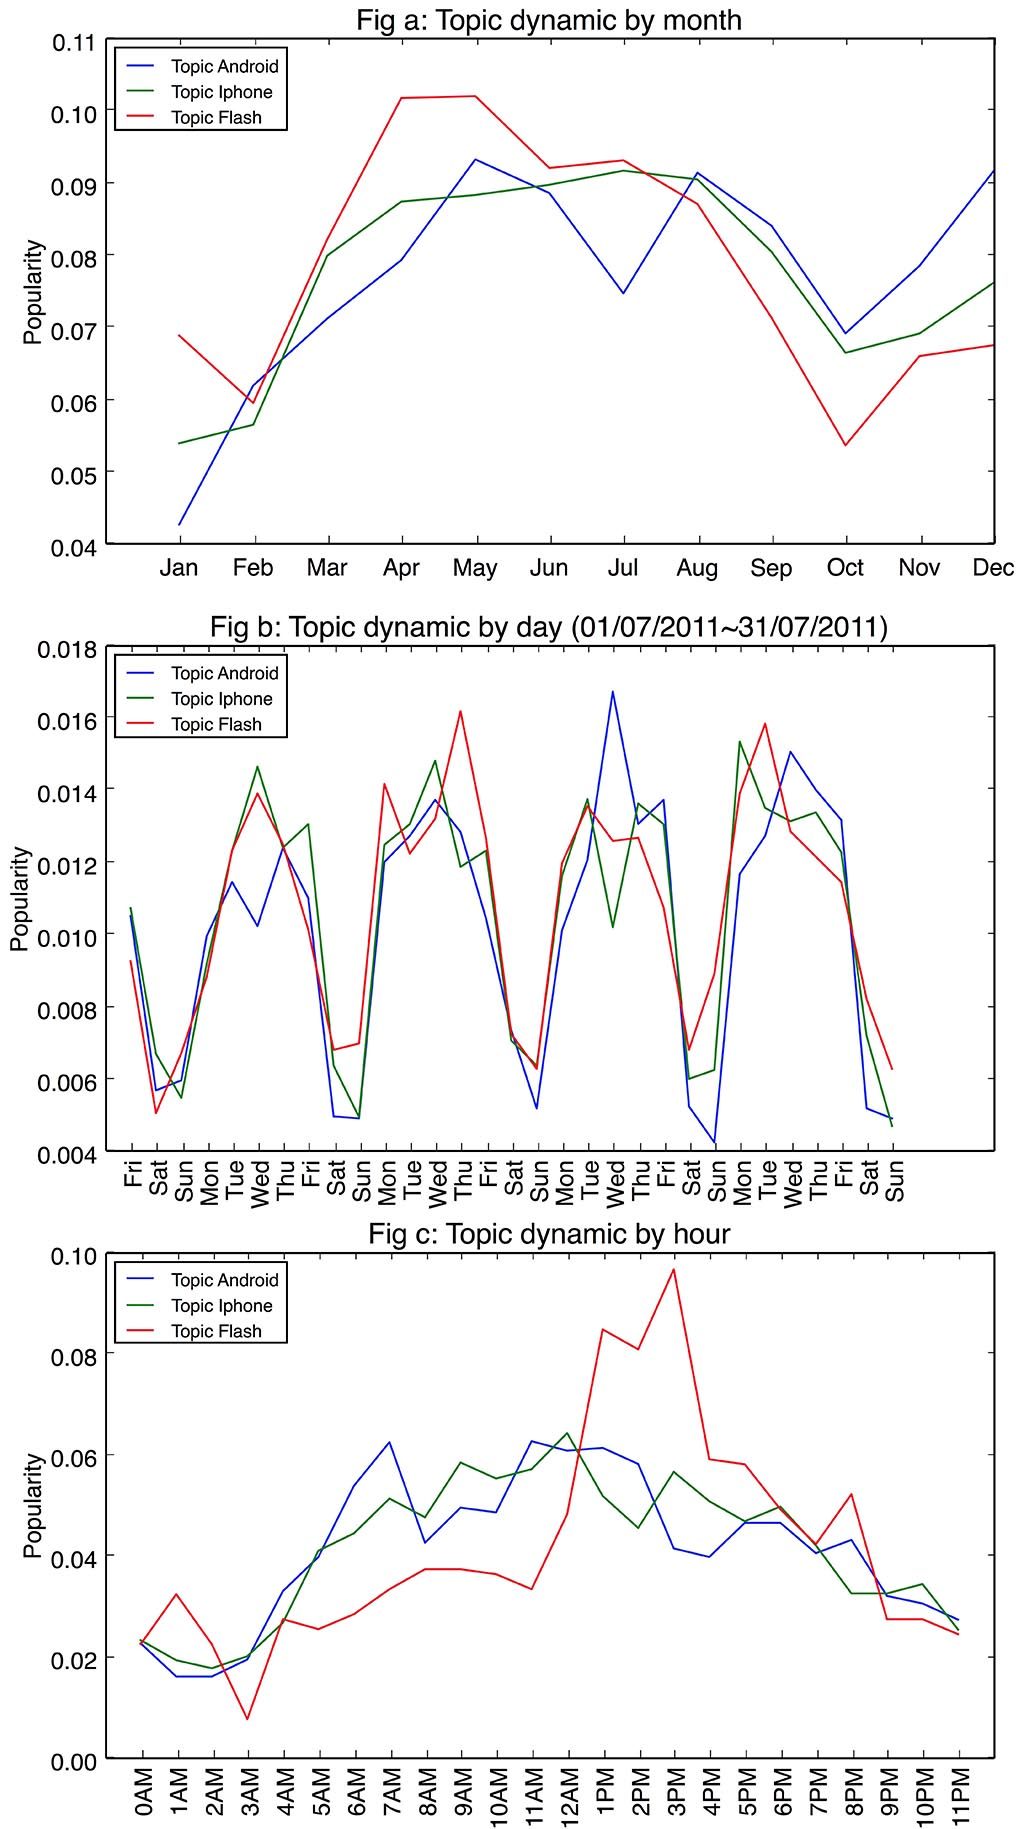
\includegraphics[width=5in]{timelevelv2.jpeg}  
\caption{Topic dynamics}
\label{fig:timelevel} 
\end{figure}
\begin{figure}
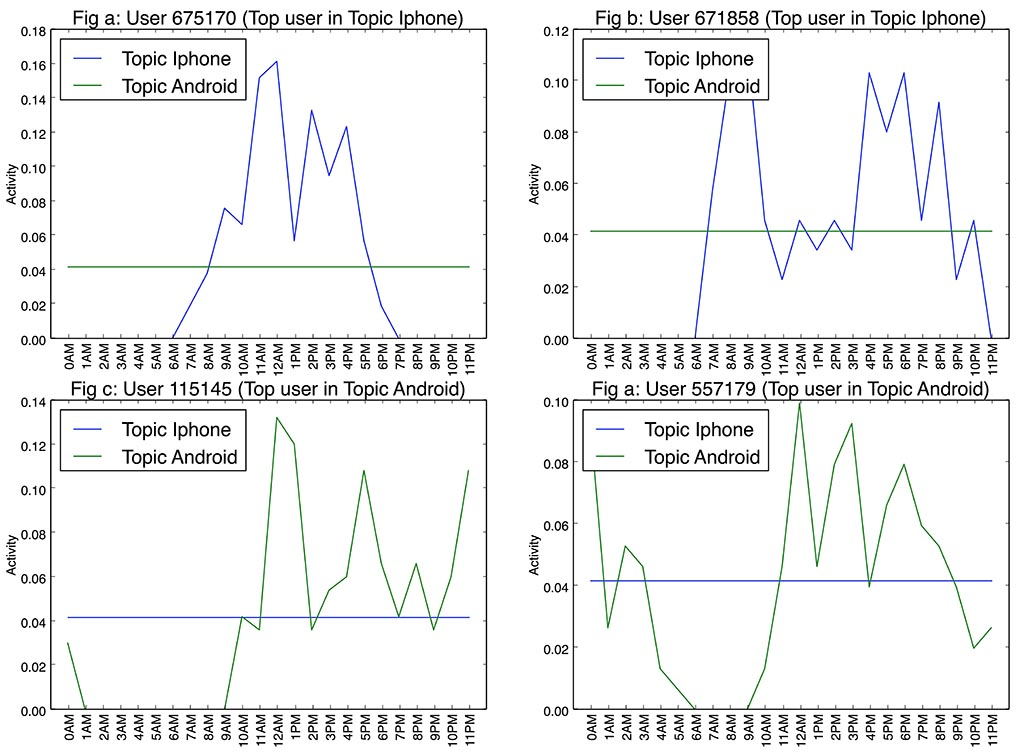
\includegraphics[width=5in]{timeusersmall.jpg}  
\caption{User Topic Activities}
\label{fig:usertimelevel} 
\end{figure}






\section{Summary: an effective model to extract expertise and temporal indications}
In this chapter, we addressed the problem of topic detection, activity modeling, temporal modeling and expertise detection in Q\&A sites. We presented the TTEA (Temporal Topic Expertise Activity) model that simultaneously uncovers the topics, activities, expertise and temporal dynamics. This extracted information enables us to improve tasks such as: question routing, expert recommending and community life-cycle management. We demonstrated that TTEA shows advantages in topic modeling. It also achieves good performances on question routing task and expert detection task compared with the state of the art models. There are still many future directions for this work, for instance, our model is obviously not limited to Q\&A datasets and we intend to adapt it to other kinds of social media.


\chapter{Conclusion}
\doublespacing
\label{chap:intro}
\minitoc

\section{Summary of contributions}
Although the Web always was a social object, the Web 2.0 evolution allowed users to very easily interact and collaborate with each other in a social media platform as creators of user-generated content and members of communities and social networks. When analyzing the social Web activities and productions, it is crucial to jointly consider both aspects: the user-generated contents and the user-generated interactions.

In this thesis, we proposed a framework, which combines social network analysis, social media mining and semantic web technologies, to help manage user-generated content websites. The main motivating scenario for our research was the case of question-and-answer sites (Q\&A sites), which is a very rich and special case of user-generated content (UGC) website and (implicit) communities of interests. Through the archived questions and answers Q\&A sites rapidly became huge repositories of potentially reusable knowledge requiring efficient search and access means. They also capture social interactions and structures that can help navigate the knowledge repository by providing interest and expertize indicators.

Therefore we addressed several research questions such as:
\begin{itemize}
\item{How to formalize user-generated content? How can we identify the common topics binding users together?}
\item{How can we generate a semantic label for topics? How can we detect topic-based overlapping communities?}
\item{How can we extract topics-based expertise and temporal dynamics?}
\end{itemize}

To answer these research questions, we conducted a study on a data set from the popular question answer site Stack Overflow. 
First we designed reused and designed Semantic Web schemas to formalize both the explicit information such as user-generated content and the implicit information such as detected communities, topics and temporal dynamics obtained as a result of our analysis.
Then we applied the original LDA model as a first approach to extract these implicit information from the original user-generated content. Based on the results and performances, we extended our work in three directions:

\begin{itemize}
\item{Firstly, we addressed the efficiency problem of the original LDA model.}
\item{Secondly we automatically generated semantic labels for bag of words which is the output of the original LDA model.}
\item{Thirdly, we proposed a new LDA model supporting the extraction of temporal trends and expertise indicators from user-generated content.}
\end{itemize}

To summarize we consider the major contributions of this thesis are:
\begin{itemize}
\item{\textbf{How to formalize user-generated content?} We designed a prototype system to formalize both implicit and explicit information in question answer site, to extract the implicit information from the original explicit user-generated content, and to provide useful services by using these detected information. Besides, we proposed a vocabulary used to formalize the detected information.}

\item{\textbf{How can we identify the common topics binding users together?} We present a topic tree distribution method to extract topics from tags. We also propose a first-tag enrichment method to enrich questions which only have one or two tags. We show the effectiveness and efficiency of our topic extraction method.}

\item{\textbf{How can we generate a semantic label for topics?} We propose and compare metrics and provide a method using DBpedia to generate adequate labels for a bag of words capturing a topic.}

\item{\textbf{How can we detect topic-based overlapping communities?} Based on our topic extraction method, we present a method to assign users to different topics in order to detect overlapping communities of interest.}

\item{\textbf{How can we extract topics-based expertise and temporal dynamics?} we present a joint model to extract topic-based expertise and temporal dynamics from user-generated content. We also propose a post-processing method to model user activity. Traditionally, this information has been modeled separately.}

\end{itemize}

%TODO FAB: No screenshots of your prototype? nothing on the application you targeted?

These results were published in international conferences and journals:
%TODO FAB: add the list of your publications in chronological order with a one sentence summary of the paper for each item

\begin{itemize}

\item{Zide Meng, Fabien L. Gandon, Catherine Faron-Zucker: Overlapping Community Detection and Temporal Analysis on Q\&A Sites. Journal of Web Intelligence and Agent Systems 2016. }. 

\item{Zide Meng, Fabien L. Gandon, Catherine Faron-Zucker: Joint model of topics, expertises, activities and trends for question answering Web applications. IEEE/WIC/ACM Web Intelligence 2016.}

\item{Zide Meng, Fabien L. Gandon, Catherine Faron-Zucker, Ge Song: Detecting topics and overlapping communities in question and answer sites. Journal of Social Network Analysis and Mining 5(1): 27:1-27:17 (2015)}


\item{Zide Meng, Fabien L. Gandon, Catherine Faron-Zucker: Simplified detection and labeling of overlapping communities of interest in question-and-answer sites. IEEE/WIC/ACM Web Intelligence 2015}


\item{Zide Meng, Fabien L. Gandon, Catherine Faron-Zucker, Ge Song: Empirical study on overlapping community detection in question and answer sites. IEEE/ACM ASONAM 2014: 344-348}

\item{Zide Meng, Fabien L. Gandon, Catherine Faron-Zucker: QASM: a Q\&A Social Media System Based on Social Semantic. International Semantic Web Conference (Posters \& Demos) 2014: 333-336}
\end{itemize}

\section{Perspectives: current limitations and future work}

We can group current limitations and perspective according to the research questions we addressed:
\begin{itemize}
\item{\textbf{How to formalize user-generated content?}
We only considered formalizing implicit and explicit information of social media websites, especially question answer sites. However, people are using different kinds of social media websites at the same time. We did not conduct research on how to formalize and integrate several social media websites and extract implicit information from the integrated view. For instance a user who showed a interest in economy topics on Youtube may also be interested in the same topic on other platforms. Likewise, a user decreasing his activity in one social media site may indicate a decreasing activity in other social media site (e.g. busy time) or not (e.g. shifting platforms).}

\item{\textbf{How can we identify the common topics binding users together?} We designed an efficient method to extract topic from tags on question answer sites. However, some social media site do not support social tagging on user-generated content. A solution could be to study how to automatically select several keywords or tags for user-generated content and how existing approaches for these questions combine with our analysis.}

\item{\textbf{How can we generate a semantic label for topics?} We use DBpedia as external knowledge to help generate labels capturing the meaning of topics. A key step of our method is to link the words of a topic to DBpedia. However, many of these words have no links to the DBpedia knowledge base. One solution could be using more linked open data sources to obtain more links.}

\item{\textbf{How can we detect topic-based overlapping communities?} The social network on question answer site is different with traditional relation-based social network. Users are focusing more on the contents rather than links between them. However, for some social media site, users are interacting and maintaining explicitly social links. In these cases, a perspective would be to combine graph-based overlapping community detection methods with our method.}

\item{\textbf{How can we extract topics-based expertise and temporal dynamics?} It is obvious that the proposed models and methods are not limited to the processing of Q\&A data set. We should study how to apply and adapt our model to other kinds of social media websites. In addition, we do not make full use of the extracted user and topic temporal information. A potential work could be combining all the extracted information to optimize question routing and user recommendation tasks and in general provide new functionalities to community managers.}

\end{itemize}





\appendix

\chapter{Appendix}
\label{chap:appendix}

\section{Survey Example}

\subsection{Survey Title}
Topic Labelling Survey-A
\subsection{Survey Description}
We are studying algorithms to generate a global label for a bag of words representing a topic discussed in a forum.
To help us in this study, we invite you to participate to this topic labelling survey.
Each question below refers to one bag of words from a real forum topic (e.g. Topic 1 - Bag of words: "css, html, firefox, ie, internet-explorer, browser, xhtml, web-development, div, layout") and several options for a possible label for that topic (e.g. html, firefox,web-development, css, browser")
Please choose one option which can represent the best label for that topic.
If you find none of the proposed labels is adequate (i.e. if the labels do not well describe the topic in your opinion), please specify your own label using the "Other" label field.
Thank you very much for your participation.
\subsection{Survey Content: An example}
Topic 1 - Bag of words: "css, html, firefox, ie, internet-explorer, browser, xhtml, web-development, div, layout" Possible labels: 
\begin{itemize}
    \item html
    \item firefox
    \item web-devlopment
    \item css
    \item browser
    \item other
\end{itemize}


\bibliographystyle{ThesisStyle}
\bibliography{Thesis}

%\printnomenclature

% \cleardoublepage
% \begin{vcenterpage}
% \noindent\rule[2pt]{\textwidth}{0.5pt}
% \begin{center}
% {\large\textbf{Temporal and semantic analysis of richly typed social networks from user-generated content sites on the web\\}}
% \end{center}
% {\large\textbf{Abstract:}}


% {\large\textbf{Keywords:}}
% Overlapping community detection, Temporal analysis
% \\
% \noindent\rule[2pt]{\textwidth}{0.5pt}
% \end{vcenterpage}

\end{document}
